\def\gsim{\mathrel{
\rlap{\raise 0.511ex \hbox{$>$}}{\lower 0.511ex
\hbox{$\sim$}}}}
\def\lsim{\mathrel{
\rlap{\raise 0.511ex \hbox{$<$}}{\lower 0.511ex
\hbox{$\sim$}}}}

\FloatBarrier
\subsection{Introduction}
Some three hundred years after Galileo observed the Jovian
satellites, the twentieth century heralded a new era in
observational astronomy with  radio and microwave antennas and
gamma- and X-ray detectors, which revolutionized astronomy and
opened the entire electromagnetic spectrum for observing
and understanding the Universe. Each new spectral window
has unveiled a new source or phenomenon that could not have been
discovered in any other way. A remarkable revelation
coming from these observations is that about 96 percent of
our Universe is invisible and that gravitational interaction
powers the most luminous and spectacular objects and phenomena
such as quasars, gamma-ray bursts, ultra luminous X-ray sources,
pulsars, and the evolution of the early Universe. Gravity has,
so far, played a passive role. But that is about to change.

Einstein's General Theory of Relativity is among the most 
successful physical theories of the 20th century. It has
passed with flying colours all laboratory-based experiments
and solar system tests.  It predicts that dynamical systems 
in strong gravitational fields will release vast amounts of 
energy in the form of gravitational radiation (see Box 
\ref{box:gw} for a brief introduction to gravitational waves).
This radiation has the potential to open a new window on the Universe, 
complementing the electromagnetic window. Russell Hulse 
and Joseph Taylor were awarded the 1993 Nobel Prize in Physics for 
their discovery of a binary consisting of two neutron stars in 
close orbit, in which indirect evidence for the emission of
gravitational waves (GWs) was found. 

\FloatBarrier
\subsection{Executive Summary}
Gravitational waves interact weakly with matter because gravity 
itself is very weak.  Detectable amounts of gravitational 
radiation cannot be produced in a laboratory but catastrophic 
astronomical events could be the source of strong GWs.
The first attempts to detect cosmic gravitational radiation were made in 
the 60's by Joseph Weber, who built resonant bar detectors, but they were 
not sensitive enough to even the most energetic sources of gravitational 
waves, such as a nearby supernova.  Over the past four 
decades, progress in technology has led to the construction of 
ever more sensitive instruments, culminating in long-baseline
laser interferometric detectors such as the
European GEO\,600 and Virgo and the American LIGO.

Interferometric detectors that are currently
taking data, and advanced detectors that will be built over the next 
five to ten years, will be the first steps in establishing the field of 
{\em gravitational astronomy.} Advanced Virgo and LIGO are expected 
to observe several tens of inspiralling and merging binaries of 
neutron stars (NSs) and black holes (BHs) each year. They could also detect 
occasional Galactic sources such as transients associated with supernovae, 
glitching pulsars, or soft gamma-ray bursts.
This phase of observation will, for the first time, test 
Einstein's theory in the dissipative regime beyond the basic quadrupole 
approximation, verify the existence of binary black holes (BBHs), measure the 
speed of gravitational radiation relative to the speed of light and map 
the expansion rate of the Universe on scales of hundreds of megaparsec (Mpc), 
providing a completely independent estimate of the Hubble parameter. 

Advanced Virgo and LIGO will be sensitive to binary neutron stars (BNSs)
at a distance of 200\,Mpc and to stellar mass BBHs
at a red shift of $z=0.5.$ The lower frequency cutoff of a detector 
places an upper limit on the total mass of binary systems they can 
detect. A lower frequency cutoff of 20\,Hz in the case of Virgo and LIGO
limits the total mass to be less than about $200\,M_\odot.$ 
ET plans to improve the amplitude sensitivity by an order of magnitude 
and extend the frequency sensitivity down to 1\,Hz. This will allow
astronomers to explore binaries at cosmological distances and
unveil new sources: ET would observe BNS
up to a redshift of $z\sim 2,$ stellar-mass BBH
population at the edge of the Universe ($z\sim 15$) and 
intermediate-mass ($10^2$--$10^4\,M_\odot$) BBH out to a typical
redshift limit $z\sim 5$. ET will be sensitive to supernovae out to a
distance of 15 million light years within which one might expect to
observe an event every year. 

An observatory with the capability of ET will produce tremendous scientific 
payoffs.  ET will make it possible to observe a greater variety of 
phenomena and provide a new tool for expanding our knowledge of fundamental
physics, cosmology and relativistic astrophysics. ET's key science
objectives are:

\paragraph {\bf Fundamental Physics and Gravity}
\begin{enumerate}
\item {\em Is the nature of gravitational radiation as predicted by 
Einstein's theory? }

ET will allow a test of the wave generation formula beyond the quadrupole 
approximation and check whether 
there are only two polarizations as predicted by Einstein's theory or six as 
in scalar tensor theories. It could accurately measure the GW propagation 
speed by coincident observation of GW and EM radiation from BNS
coalescences at $z\sim 2$ and constrain the graviton mass.

\item {\em Are black hole spacetimes uniquely given by the Kerr geometry?}

By measuring different quasi-normal modes, ET will test if 
the spacetime geometry of a BH is uniquely described by its mass and spin.
% \footnote{Although astronomical black holes could have electric charge 
% it is expected that any residual charge would be quickly neutralized.} 
Additionally, ET can measure the multipole moments of a source from the 
radiation emitted as a stellar-mass BH spirals into an 
intermediate-mass BH and confirm if the different moments 
depend only on the massive BH's mass and spin.

\item {\em What is the physics of gravitational collapse?}

ET can study supernovae and explore if they leave behind a massive 
object that is trapped inside an event horizon or lead to a naked 
singularity, or some other exotic object. ET could well reveal a new 
class of objects and phenomena, for instance \emph{silent supernovae} 
\cite{Woosley:1992} and other gravitationally unstable transients.

\item {\em What is the equation of state of matter at 
supra-nuclear densities as might be found in NS cores?}

The equation of state (EoS) of NSs affects the late-time evolution of 
BNS and neutron star-black hole (NSBH) binaries. By matching the observed 
radiation from the coalescence of such sources to theoretical predictions, ET will 
deduce the EoS of NS cores.

\item {\em What is the maximum mass of a neutron star?}

The maximum mass of a white dwarf is $\sim 1.4\,M_\odot$ as determined 
by the electron degeneracy pressure.  The maximum mass of a NS is an 
additional test of the nature of matter at extremely high densities; 
it is currently unknown and should be determined by accurately
constructing their mass function from millions of BNS systems observable
in ET.

% \item Are there really ten spatial dimensions? 
% \item What is the nature of quantum gravity and what is the origin of space and time? 
\end{enumerate}
\paragraph {\bf Cosmology}
\begin{enumerate}
\item {\em What are the true luminosity distances of cosmological sources?}

BBH and BNS binaries are an astronomer's ideal {\em standard candles}
or, more appropriately, {\em sirens}.
Gravi\-tational wave observations alone can determine both the 
apparent and absolute luminosity of a source. With ET these standard sirens can
be used to calibrate the cosmic distance ladder.

%\item {\em Is the Universe isotropic and does it expand at the same rate in different 
%directions?}

%A precision measurement of the Hubble parameter will allow ET to map the 
%rate of expansion of the Universe in different directions and discover
%tiny anisotropies.

\item {\em What is the EoS of dark energy and how does it vary with redshift?}

ET could observe thousands of coalescing BNS and NSBH
systems in coincidence with optical or gamma-ray observations
and hence measure both the luminosity distance and 
redshift. ET will, therefore, facilitate precision 
measurement of the dark energy EoS and its variation with redshift.

\item {\em How did black holes at galactic nuclei form and evolve?}

ET can verify if seeds of galaxy formation were intermediate BHs
of hundreds to thousands of solar masses and map their merger history up to
redshifts of $z\sim 5$--15 depending on the total mass and mass ratio of 
progenitor binaries.

\item {\em What were the physical conditions in the primeval Universe and what
phase transitions occurred in its early history?}

Stochastic GW backgrounds could be produced by quantum 
processes in the primordial Universe or during phase transitions in its 
early history. ET will be sensitive to background densities $\rho_{\rm GW}
\gsim 10^{-12}\,\rho_c,$ where $\rho_c$ is the critical density of the Universe.

\end{enumerate}

\paragraph {\bf Astrophysics and Multimessenger Astronomy}
\begin{enumerate}
\item {\em What is the mass function of BHs and NSs and
their redshift distribution?}

ET will measure masses and spins of millions of NSs and BHs
in binary systems and will thereby obtain a census of these objects as a function of
redshift. This will be a very valuable database for understanding a host of questions
in astronomy related to redshift evolution of compact objects. 

\item {\em What are the progenitors of gamma-ray bursts?}

Gamma-ray bursts (GRBs) are the most luminous electromagnetic sources in the
Universe. While advanced detectors might provide some clues as to their
origin, ET will provide a large statistical sample of events that
could be used to understand GRB progenitors and to test their astrophysical models. 

\item {\em How do compact binaries form and evolve?}

The process by which main sequence binary stars evolve into compact 
binaries (that is, BNS and BBH)
could be understood by ET's observation of millions of coalescing
binaries with different masses, mass ratios and spins and mapping the
observed population to astrophysical models.

\item {\em What is the physical mechanism behind supernovae and how asymmetric 
is the gravitational collapse that ensues?}

Supernovae are complex processes whose modelling requires many 
different inputs, including relativistic magneto-hydrodynamics, general relativity
and nuclear and particle physics. 
ET's observation of supernovae in coincidence with EM afterglows and 
neutrinos could provide the data necessary to constrain models and help
understand the process by which stars collapse to form NSs and BHs.

\item {\em Do relativistic instabilities occur in young NSs and if so 
what is their role in the evolution of NSs?}

Non-linearities of general relativity could cause instabilities in 
NSs that lead to parametric amplification of GWs.
ET's observations of the formation of NSs can explore if such
instabilities occur in young NSs and how that might affect
their spin frequencies.

\item {\em Why are spin frequencies of NSs in low-mass X-ray binaries bounded?}

ET will verify if gravitational radiation back-reaction torque is responsible 
for the observed upper limit on NS spin frequencies in low-mass X-ray binaries.

\item {\em What is the nature of the NS crust and its interaction 
with the core?}

ET should detect NS ellipticities that are $\rm few \times 10^{-10}$
or larger depending on their spin frequency. This can be used to deduce the
property of NS crusts. ET might also detect GWs 
that are expected to be emitted when pulsars glitch and magnetars flare and thereby
help understand crust-core interaction that is believed to transfer angular 
momentum from the core to crust.

\item {\em What is the population of GW sources at high redshifts?}

A large population of point sources would produce a confusion background that would
be detectable by ET if the energy density of the background is large enough.
Detection of confusion backgrounds can be used to understand the nature and
population of GW sources in the Universe.
\end{enumerate}
%
Gravitational radiation is an essential prediction of any relativistic
theory of gravity. It will be a new tool for observing the most 
energetic processes in the Universe---processes originating
in such extremely dense environs that all other forms of radiation
and particles might be trapped. In this chapter we will look at
what new science is enabled by ET and how its low frequency 
($<10$\,Hz) sensitivity will be critical in achieving its key science objectives. 

\etbox{i}{box:gw}
{Gravitational Waves}
{At a sufficiently large distance from cosmic sources, GWs 
can be described as a small perturbation to a flat spacetime. 
The spacetime can thus be described by a metric
$g_{\alpha\beta}=\eta_{\alpha\beta}+h_{\alpha\beta},$
$|h_{\alpha\beta}|\ll 1,$ where $\eta_{\alpha\beta}={\rm Diag}(-1,1,1,1)$ 
is the flat Minkowski metric and $h_{\alpha\beta}$ is the perturbation 
due to GWs.  In a suitable coordinate system and gauge,
$h_{\alpha\beta}$ has only two independent components conventionally
called the ``plus" and ``cross" polarizations $h_+$ and $h_\times,$ 
respectively: $h_+\equiv h_{xx}=-h_{yy},$ $h_\times \equiv  h_{xy} = 
h_{yx} $, all other components being zero, $h_{0\alpha}=h_{z\alpha}=0.$ 
\\[5pt]
The apparent luminosity of radiation ${\cal F}$, at great distances 
from the source and in geometrical units in which $c=G=1$, is related to the 
time-derivative of the amplitude 
by~\cite{schutz.2009}:
%
\begin{equation}\label{eq:flux}
{\cal F} \sim {| \dot h |^2}/{(16 \pi)}.
\end{equation}
%
If a source at a distance $D$ radiates away energy $E$ in a time $T$, 
predominantly at a frequency $f$, then writing $\dot h= 2\pi f h$ and 
noting that ${\cal F}\sim E/(4\pi D^2T)$, the amplitude of GWs is
%
\begin{equation} \label {eq:amplitude}
h \sim \sqrt{E/T}/(\pi f D) .
\end{equation}
%
Gravitational waves cause a strain in space as they pass. The distance
$L$ between two masses will be altered by an amount $\delta L$ that
is proportional to a linear combination of the two polarizations. 
Figure \ref{fig:pol} below depicts how a ring of free particles responds to
the two polarizations. 
\begin{figure}[H]
\centering
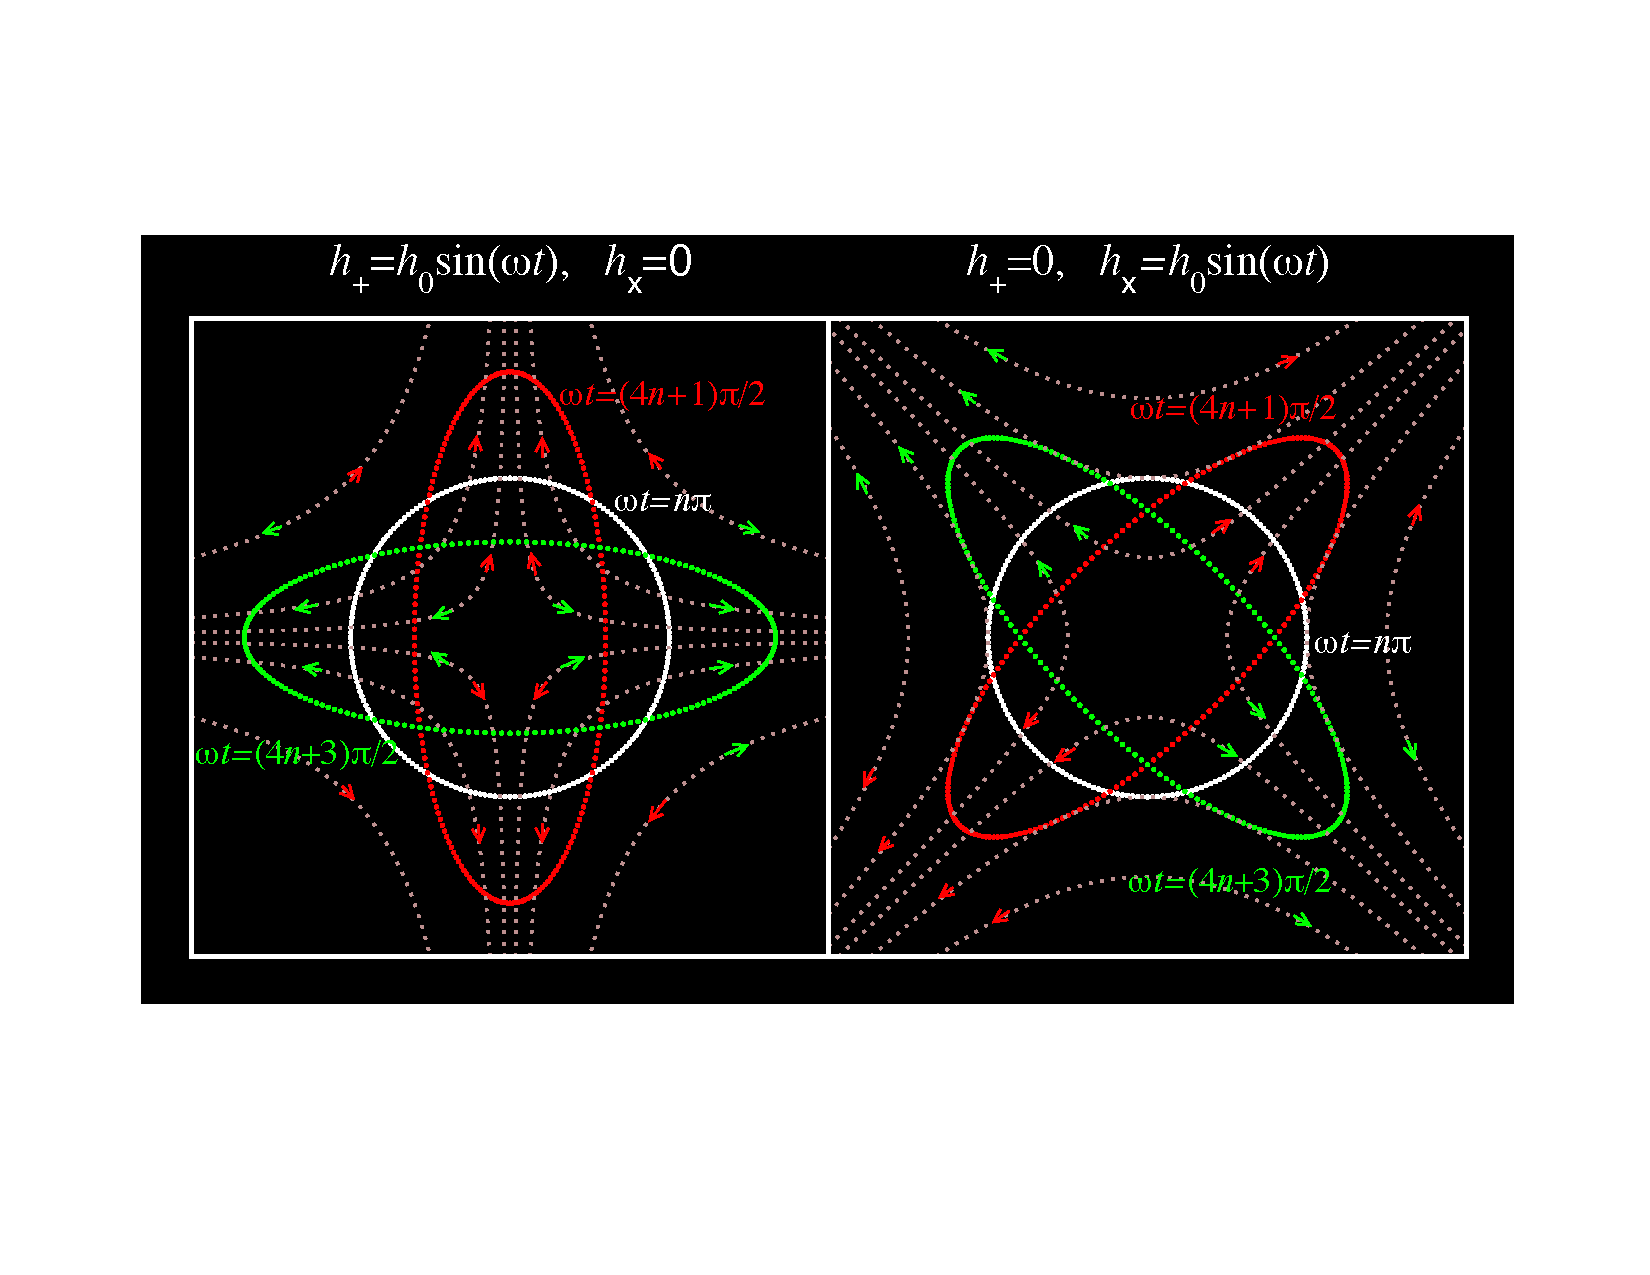
\includegraphics[width=0.95\textwidth]{./Sec_ET_ScienceCase/polarization.pdf}
\vskip 0.3cm
\caption{Response of a circular ring of free particles to a passing sinusoidal 
GW of plus (left) or cross (right) polarization.
The tidal field of the waves on the ring is indicated by light dotted 
lines. The direction of the force reverses sign each half-period of 
the wave as indicated by the red  and green arrows. The ring oscillates between
the red and green ellipses over one period of the wave, the maximum 
eccentricity of the ellipses being the wave amplitude $h_+$ or $h_\times$. 
A general wave is a linear combination of the two polarizations.
}
\label{fig:pol}
\end{figure}
\vskip -0.6cm
A sinusoidal wave incident perpendicular to the plane of the ring tidally 
deforms it into an ellipse over the first quarter of the wave's period, back 
to the ring over the next quarter, to an ellipse oriented orthogonally to the 
first over the third quarter, and back to the ring over the fourth quarter. 
}

\clearpage 

\subsection{Sources of gravitational waves in ET}

The goal of this Section is to give an overview of the sources
expected to be observed by ET and the problems that were addressed 
in the context of the Design Study. A brief description of how ET 
responds to an incident GW is given in Box~\ref{box:response}.
ET will observe GWs from a variety of different astronomical 
sources such as BNSs, BBHs, supernovae, spinning NSs,
glitching pulsars, flaring magnetars, and, perhaps, a primordial 
stochastic background.
We will first give a brief introduction to the types of sources
expected to be routinely observed by ET. This will be followed
by a discussion of the fundamental physics, 
astrophysics and cosmology enabled by ET. Recent reviews on sources
and science can be found in Sathyaprakash and Schutz \cite{lrr-2009-2}
and Andersson et al \cite{2011GReGr..43..409A}.

\etbox{i}{box:response}
{ET's Response to Gravitational Waves}
{
A single interferometric gravitational-wave detector cannot 
measure both polarizations of GW, but only a linear combination of the
two, called the \emph{response} $h(t)$, given by
\begin{equation}
h(t) = F_+(\theta,\, \varphi,\, \psi) h_+(t) +
       F_\times(\theta,\, \varphi,\, \psi) h_\times(t).
\label{eq:response}
\end{equation}
Here, $F_+$ and $F_\times$ are the detector antenna pattern functions,
$\psi$ is the polarization angle, and $(\theta,\,\varphi)$ are angles
describing the location of the source on the sky (see \emph{e.g.}\ 
Ref.~\cite{lrr-2009-2} for details). The various angles can be treated as
constants for transient sources, but must be taken to be 
time-dependent for sources that last for more than about 30 min, after
which Doppler modulation of the signal due to the relative motion 
of the source and detector cannot be neglected.
\\[5pt]
It is expedient to write the response as
\begin{equation}
h(t)=F(t)\left(\cos\xi\,h_+ + \sin\xi\,h_\times\right),\quad
F=\sqrt{F_+^2+F_\times^2},\quad \tan\xi=F_\times/F_+.
\end{equation}
It turns out that $F$ is independent of the polarization angle and
so measures the sensitivity of the detector to different locations on
the sky.  Figure \ref{fig:response} below plots $F(\theta,\,\varphi)$
for an L-shaped interferometer such as Virgo (panel on the left) 
and for a triangular ET (panel on the right). Since ET consists of 
a triangle of three detectors, it is a factor $\sqrt{3}$ more sensitive 
than a single detector; but, since the opening angles of the 
arms are $\pi/3,$ the sensitivity is smaller by a factor $\sin (\pi/3)= \sqrt{3}/2$ 
compared to an L-shaped detector---an overall factor of 3/2, as 
can be seen in Fig.~\ref{fig:response}.
\begin{figure}[H]
\centering
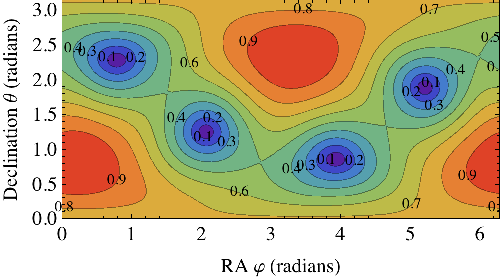
\includegraphics[width=0.495\textwidth]{./Sec_ET_ScienceCase/Virgo-AP.pdf}
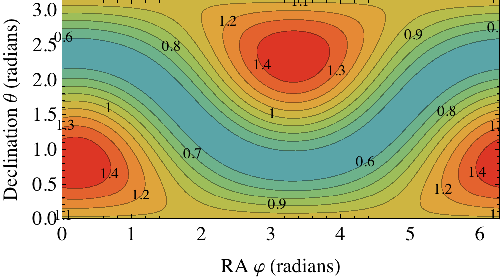
\includegraphics[width=0.495\textwidth]{./Sec_ET_ScienceCase/ET-AP.pdf}
\vskip 0.3cm
\caption{Antenna pattern of ET (right panel) compared to that of
Virgo (left panel). ET is assumed to be at the same location as
Virgo. Note that Virgo is a {\em single} L-shaped detector while
ET consists of {\em three} V-shaped interferometers rotated relative 
to one other by 120 $\deg.$ The combined antenna pattern of the three detectors 
in ET (defined as $F^2=\sum_{A=1}^3\,F_A^2$, where $F_1,F_2,F_3$ are the
individual antenna pattern functions) makes the response the same for all 
sources whose sky location makes the same angle to the plane formed 
by ET (see \emph{e.g.}\ contours marked 0.6).}
\vskip -0.3cm
\label{fig:response}
\end{figure}
}
\subsubsection{Compact binary coalescences}
\label{sec:binaries}

\begin{figure*}
\centering
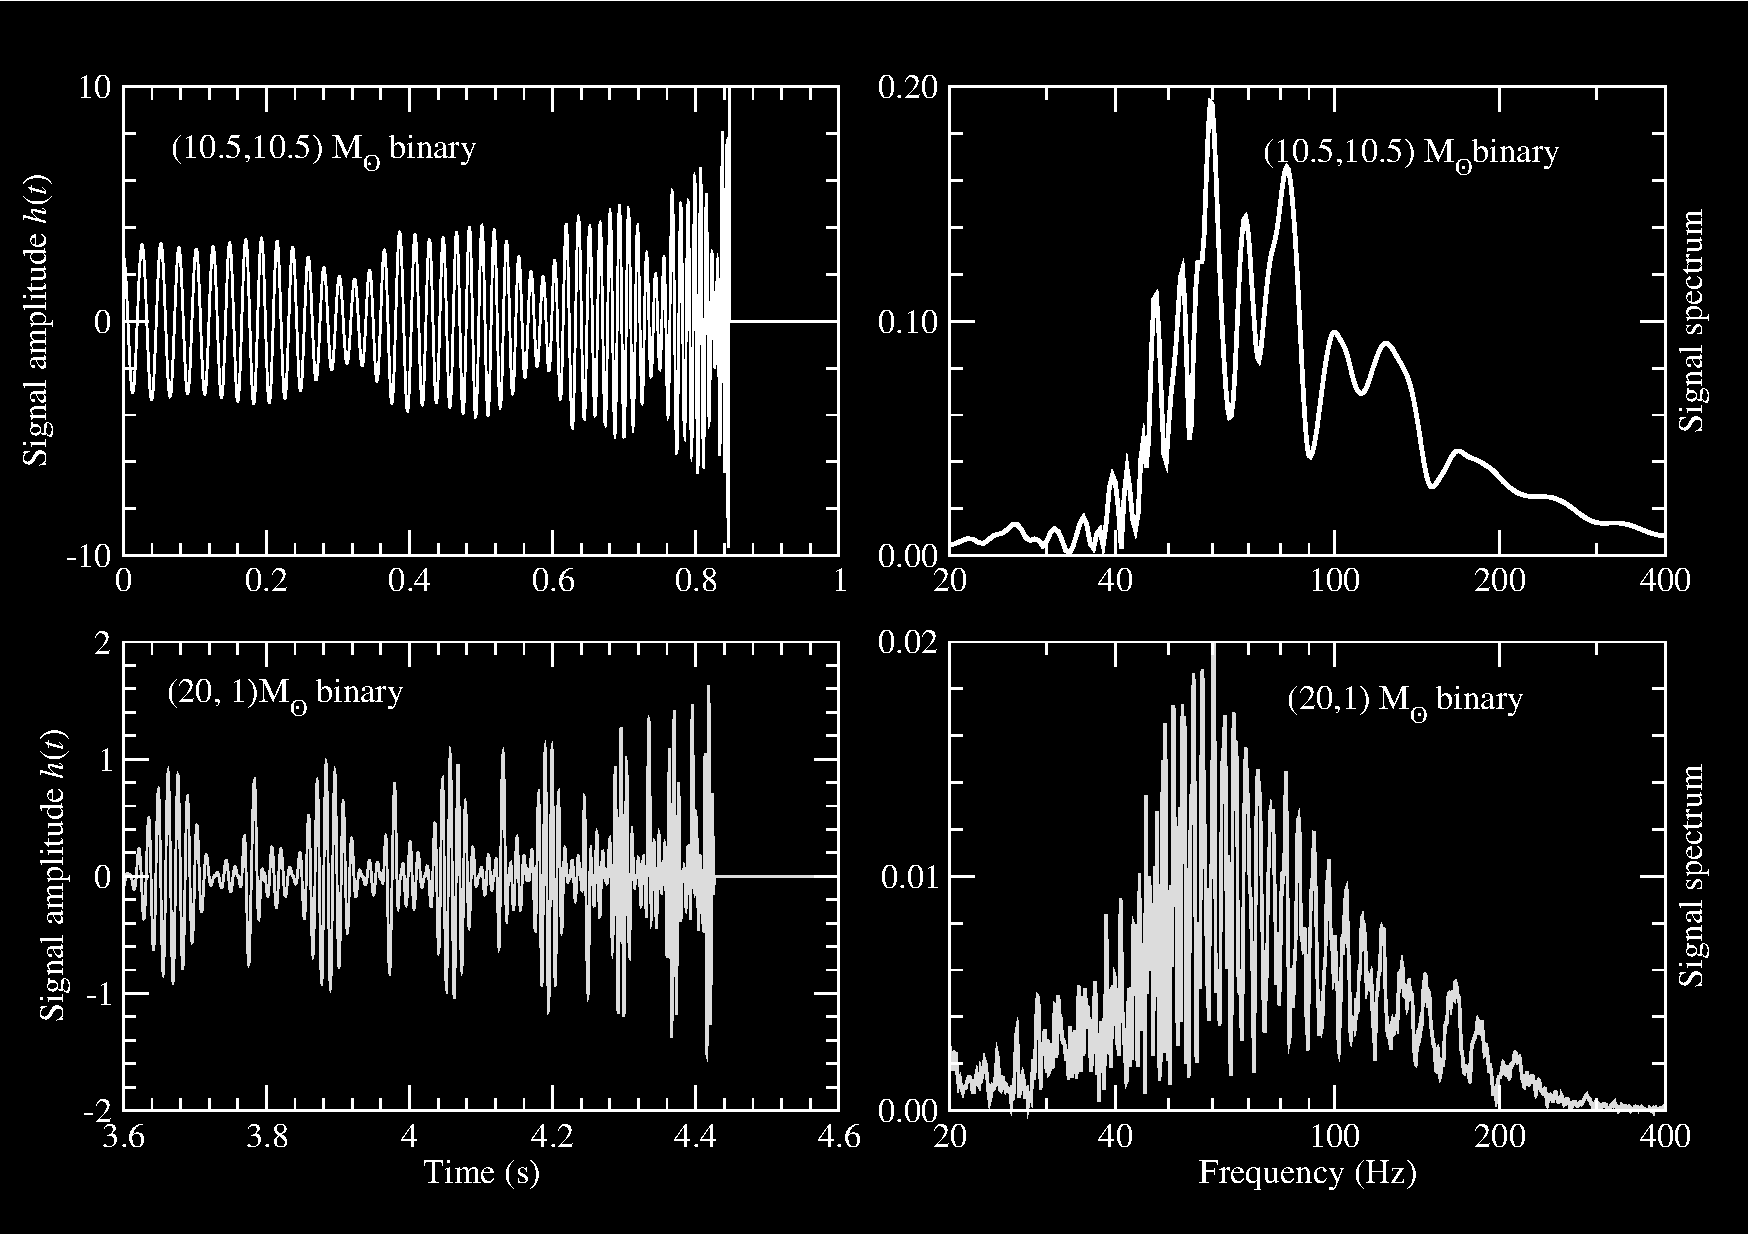
\includegraphics[width=0.99\textwidth]{./Sec_ET_ScienceCase/spinningBinaries.pdf}
\caption{The waveforms from two compact binary systems that ET could
detect. Left panels show the time-domain waveforms (for clarity only the
last second is plotted), right panels show the frequency spectrum. 
The upper two panels show a binary composed of two equal masses; the 
waveform's modulation is due to interaction between the spins of the bodies 
and the orbital angular momentum. The lower panels show a binary 
composed of a neutron star and a black hole. In this case, the signal 
amplitude is smaller, the duration is longer due to the larger mass ratio, 
and the signal modulation is stronger as the spin-orbit precession of the 
orbital plane is greater.}
\label{fig:chirps}
\end{figure*}

A compact binary, consisting of NSs and/or BHs,
evolves by emitting gravitational radiation which extracts rotational energy 
and angular momentum from the system. This causes the two bodies to
inspiral toward each other and eventually merge. The dynamics of a compact 
binary can be described in three phases:
\begin{itemize}
 \item The \emph{inspiral phase} in which the
system spends hundreds of millions of years. During this phase the luminosity
in GW is low and the dynamics can be solved using approximation
methods --- the most popular being the post-Newtonian (PN) approximation
(see Box~\ref{box:pn}). The two polarizations are given at the lowest order
approximation by Equations (\ref{eq:amps}), Box \ref{box:pn}. At the dominant
PN order, the frequency of the emitted signal is twice the orbital frequency;
the signal has a characteristic shape, with slowly increasing amplitude and 
frequency, called a \emph{chirp} waveform. A BNS system will stay in
ET's sensitivity band for nearly a week starting from 1\,Hz, 20 hours starting from
2\,Hz, and a little less than 2 hours starting from 5\,Hz. For the same lower frequency 
limits the duration of a BBH signal from a pair of 10$\,M_\odot$ BHs is 2 days, 
45 minutes and 4 minutes, respectively. Such long durations, owing primarily 
to the low frequency sensitivity of ET, are crucial in obtaining very accurate 
estimates of a binary system's parameters, which is essential to achieve some 
of the scientific goals of ET.

When the binary companions are spinning, the signal is modulated due to 
spin-orbit and spin-spin couplings as in Fig.\ \ref{fig:chirps}. These modulations
encode the parameters of sources (their masses, spins, inclination of the orbit,
etc.) most of which can be extracted very accurately 
\cite{Arun:2005,Vecchio:2003tn,vanderSluys:2008qx,Lang:1900bz} by matching 
the observed signals onto general relativistic predictions.

At higher PN orders, the signal also contains other harmonics of the orbital
frequency and including these in the estimation of parameters has proved to
be extremely important, especially for localizing the source on the sky
\cite{VanDenBroeck:2006ar,Broeck2007,Arun:2007hu}.


\etbox{i}{box:pn}
{Post-Newtonian Description of the Inspiral Signal}
{
The adiabatic evolution of a compact binary, during which the
emission of GWs causes the component stars
of the system to \emph{slowly} spiral in towards each other,
can be computed very accurately using the 
PN expansion of the Einstein equations. Currently, the
dissipative dynamics is known  to order
$(v^7/c^7),$ where $v$ is the characteristic velocity in
the system.
\\[5pt]%\indent
For a binary consisting of two stars of masses $m_1$ and
$m_2$ (total mass $M\equiv m_1+m_2$ and symmetric mass ratio
$\nu\equiv m_1m_2/M^2$), at a luminosity distance $D_{\rm L}$,
the dominant parts of the two polarizations are given by
%%\begin{widetext}
\begin{subequations}
\label{eq:amps}
\begin{align}
h_+(t) & = \frac{2\nu M}{D_{\rm L}}(1 + \cos^2\iota)
\left [M\omega(t;t_0,M,\nu) \right ]^{\frac{2}{3}} \cos \left [2\Phi(t; t_0, M,\nu) + \Phi_0 \right ],\\
h_\times(t) & = \frac{2\nu M}{D_{\rm L}}2\cos\iota\,
\left [M\omega(t;t_0,M,\nu) \right ]^{\frac{2}{3}} \sin \left [2\Phi(t;t_0, M,\nu) + \Phi_0 \right ],
\end{align}
\end{subequations}
%%\end{widetext}
where $\iota$ is the angle of inclination of the binary's orbital angular
momentum with the line-of-sight, $\omega(t)$ is the angular velocity
of the equivalent one-body system around the binary's centre-of-mass and
$\Phi(t;\, t_0,M,\nu)$ is the corresponding orbital phase. Parameters
$t_0$ and $\Phi_0$ are constants giving the epoch of merger and the
orbital phase of the binary at that epoch, respectively.
The orbital dynamics, and hence the phase $\Phi,$ are known to order
$(v^7/c^7)$.
% where $v$ is the characteristic velocity in the system. 
\\[5pt]\indent
The above expressions for $h_+$ and $h_\times$ contain only the dominant
terms which oscillate at twice the orbital frequency. Higher order amplitude
corrections contain other harmonics (\emph{i.e.}\  phase terms depending on
$k\,\Phi(t),$ $k=1,3,4,\ldots$). 
The above expressions are
written down for a system consisting of non-spinning components on a
quasi-circular orbit. In reality, we can assume neither to be
true. Waveforms for binaries on an eccentric inspiral orbit are
known, as are those with spin effects, but we shall not discuss them here.
\vskip 0.2cm
}

\item The \emph{merger} phase when the two stars are moving at around
a third of the speed of light and experiencing extreme gravitational fields.
A post-Newtonian approximation is not accurate when the two stars get close to
each other. To predict the dynamics of the bodies during this
phase requires the full non-linear structure of Einstein's equations,
as the problem involves strong relativistic gravity and tidal deformation
and disruption.  The merger signal lasts for a very short duration (milliseconds
in the case of stellar mass BHs, to seconds in the case of the
heaviest systems ET is likely to detect). Yet BBH have the greatest 
possible luminosity of all sources one can conjure up, exceeding the 
luminosity of the entire Universe in EM radiation in that short duration.

Numerical simulations of BBH mergers have been highly successful, and 
analytical and phenomenological models of the merger dynamics have been developed. 
Following breakthroughs in 2005 \cite{Pretorius05,Campanelli:2005dd,Baker:2005vv},
it is now possible to numerically solve the full Einstein equations for the 
last orbits that include the merger and ringdown phases, for coalescing BBH
systems with comparable component masses, and to calculate the
GW signal emitted. Subsequent dramatic progress has led both to
simulations of increasing numerical accuracy and physical
fidelity, and to the inclusion of larger numbers of GW cycles before
merger, allowing full GR waveforms to be in principle useful in searching for
BBHs of ever lower mass (see \emph{e.g.}\ Fig.~3 in~\cite{Hannam:2009rd}).

Currently efforts are focussed 
on understanding the full parameter space of BBHs
of arbitrary spins and mass ratios.  In the case of BNSs the 
merger phase is not well understood, as it is complicated by a number of unknown
physical effects, such as the EoS of NSs and their magnetic fields.

 \item The \emph{ringdown} phase when the
two systems have merged to form either a NS or BH, settling down to a
quiescent state by radiating the deformations inherited during the merger.
The emitted radiation can be computed using perturbation theory and
it consists of a superposition of quasi-normal modes of the compact object
that forms after merger. These modes carry a unique signature that depends
only on the mass and spin angular momentum in the case of BH, but depends 
also on the EoS of the supra-nuclear matter in the case of NS. Just as in the
merger phase, here too the signal lasts for a very short duration (of 
milliseconds to seconds depending on the mass of the final object) and 
consistst of two to three cycles. However, the superposition of different modes 
means that the signal can have an interesting and characteristic structure.
\end{itemize}


The merger and ringdown parts of the signal last only for a short duration yet carry
tremendous luminosity. Their inclusion in a matched filter search for binary systems  
dramatically increases the distance reach of ET, relative to the reach obtained with the
inspiral phase alone. As we shall see below, having observational access to
these later stages of the coalescence process will lead to key insights into the 
structure of NS; in the case of BH it will open up the possibility of testing gravity 
in genuinely strong-field dynamics of spacetime.

\begin{figure*}
\centering
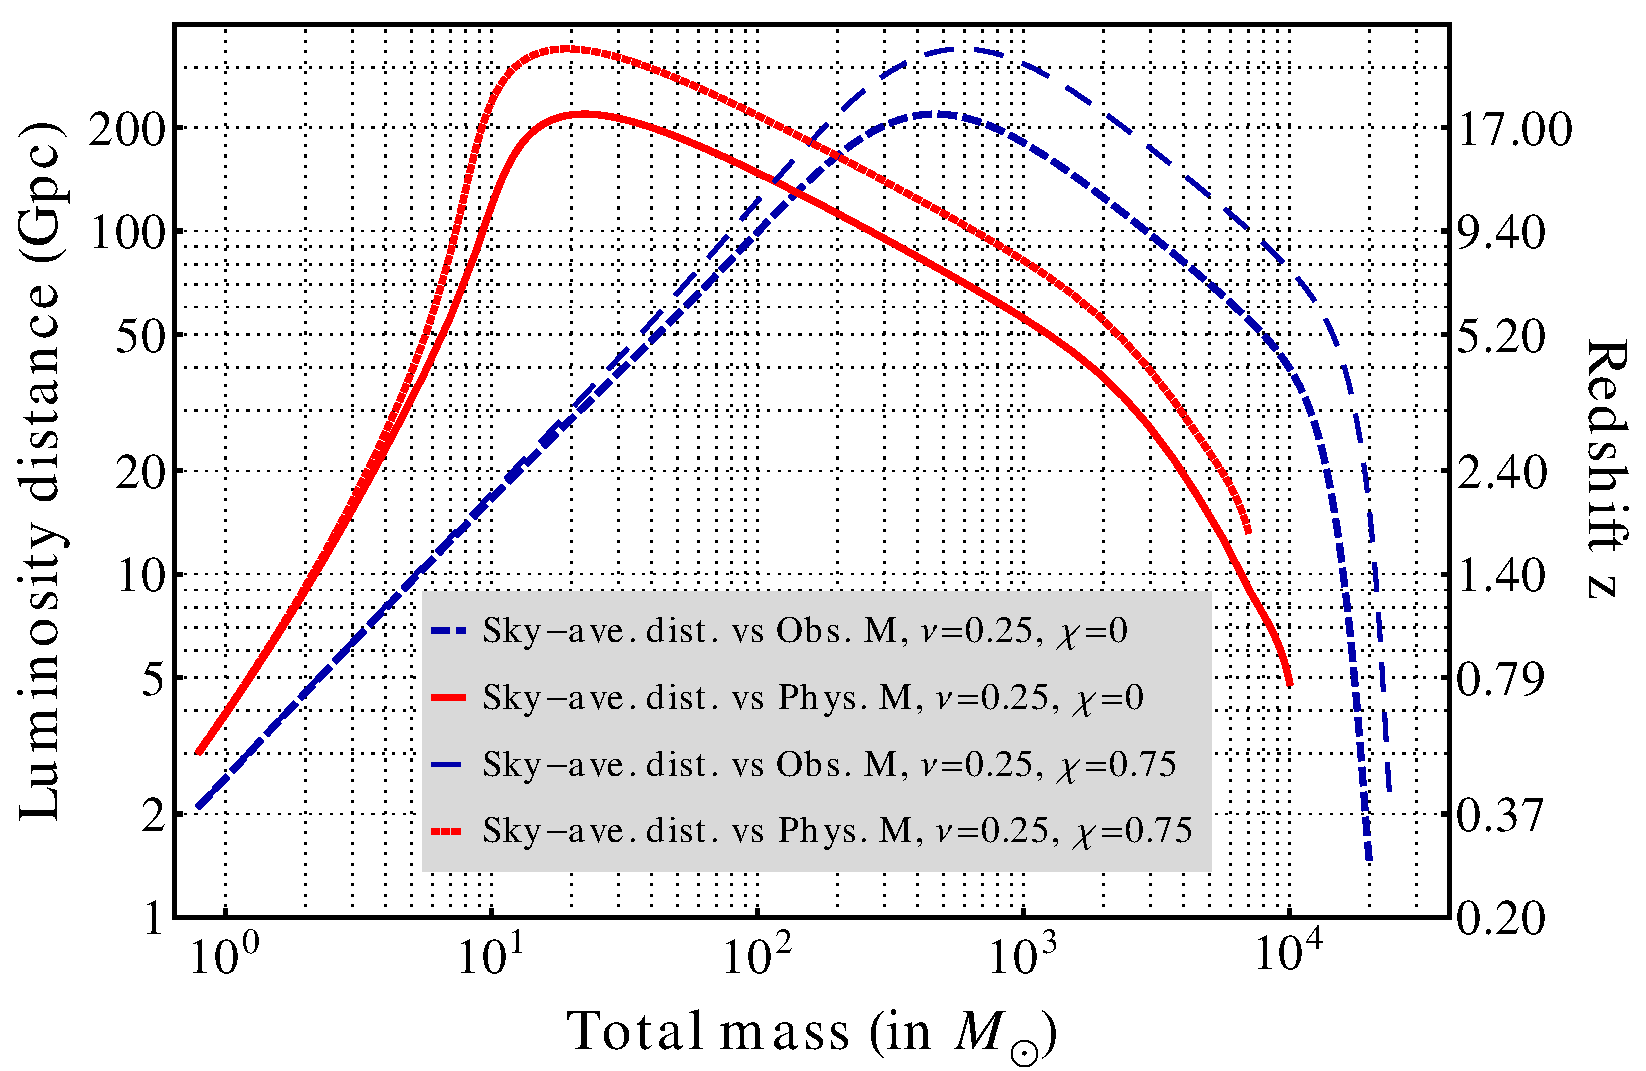
\includegraphics[width=0.75\textwidth]{./Sec_ET_ScienceCase/ET_horDist_ETB.pdf}
\caption{
ET's distance reach for signals from coalescing compact binaries as a function 
of the \emph{intrinsic} (red curves) and \emph{observed} (blue curves) total mass,
averaged over sky position and binary's orientation relative to the line-of-sight.
We assume that a source is visible if it produces an SNR of at least 8 in ET. 
Solid red and short-dashed blue curves correspond to binaries composed of 
non-spinning objects. Dotted red and long-dashed blue curves
correspond to binaries composed of objects whose spins are aligned
with the orbital angular momentum of the binary, with spin parameter $\chi=0.75$.}
\label{fig:ET_range}
\end{figure*}

\paragraph{ET's distance reach and mass range}
A standard measure of the reach of a detector is the horizon distance
$D_h$, defined as the distance at which a detector measures an SNR of 8
for an optimally-oriented and optimally-located binary, \emph{i.e.}\ overhead
from the detector and with a face-on orbit. Sub-optimally located and 
oriented sources are detected with an SNR of 8 at closer distances.

The sky-position averaged distance up to which a 3-detector ET 
observatory would detect signals from coalescing binaries with 
an SNR of 8 is shown in Fig.~\ref{fig:ET_range}, for the ET-B sensitivity 
curve (see Box\,\ref{ETSensitivityCurves}). 
The range is plotted both as a function of the intrinsic (red lines)
and observed (blue lines) total mass. The two are related by the
redshift function $z(D_{\rm L})$ as we will describe later.
The binary systems are modeled by
the phenomenological waveforms of~\cite{Santamaria:2010yb} which
comprise the inspiral, merger and ringdown stages of the coalescence.
Fig.~\ref{fig:ET_range} shows the reach associated
with two physical configurations of the
binary: equal-mass, non-spinning and equal-mass, spin-aligned configuration 
with spins $\chi_1=\chi_2=\chi=0.75$.

A neutron star binary composed of two $1.4\,M_\odot$ NSs would be 
observed by ET from a redshift of $z\simeq 2$. A NS-BH
system comprising a $1.4\,M_\odot$ NS and a $10\,M_\odot$ BH
would be observed from $z \simeq 4$. Binaries formed by stellar-mass BH
will be visible at much larger distances, allowing ET to explore their populations
at cosmological distances of $z\simeq 10$ and further. ET is also sensitive to
intermediate-mass BBHs of total mass in the range [$10^2,\,10^4]M_\odot$
over the redshift range $z\sim1$--15. ET-D's better sensitivity at lower 
frequencies compared to ET-B is important in all cases, but particularly 
so for systems with total mass in the range 500--$10^4\,M_\odot$, for which the
reach is a factor 2--10 greater for ET-D than ET-B.

\begin{table}[ht]
\begin{center}
\caption{
Expected coalescence rates per Mpc$^3$ per Myr in the local universe
($z\simeq 0$).  Also shown are predicted event rates in Advanced LIGO (aLIGO) 
and ET.}
\begin{tabular}{l|ccc}
\hline
\hline
 Source                & BNS              & NS-BH            & BBH            \\
\hline
Rate (Mpc$^{-1}$ Myr$^{-1}$)   &  0.1--6           & 0.01--0.3         & $2\times 10^{-3}$--$0.04$\\
Event Rate (yr$^{-1}$) in aLIGO & 0.4--400          & 0.2--300          & 2--4000          \\
Event Rate (yr$^{-1}$) in ET   & $\mathcal{O}(10^3$--$10^7)$ & $\mathcal{O}(10^3$--$10^7$) & $\mathcal{O}(10^4$--$10^8)$\\
\hline
\hline
\end{tabular}
\label{tab:EventRates}
\end{center}
\end{table}

\paragraph{Expected coalescence rates}
Black holes and neutron stars are expected to form after Type II 
supernovae, which occur roughly once a century in galaxies like our own.  Most stars
seem to form in binaries; a fraction of compact binary progenitors will survive the kicks that
supernovae impart, and roughly half of the remaining low-mass binaries (NSBH, BNS) will 
inspiral and eventually merge through the gradual emission of radiation. With roughly one 
Milky Way-like galaxy per 100\,Mpc$^3$, we anticipate
a rate per comoving volume $\rho_c$ large enough to permit many detections even for advanced
detectors (see Table~\ref{tab:EventRates}).
%  ROS extracts the following from PSellipticals
For example, the binary pulsar population in the Milky Way implies a local BNS merger rate 
$\rho_c^{\rm(NS-NS)}\simeq 0.2-6$\,Myr$^{-1}$\,Mpc$^{-3}$
\cite{Burgay:2003jj,Chunglee-nsns-1,Chunglee-nsns-proceedings}. 
With its vastly greater sensitivity, ET will reach deep back into the universe.
Due to an enhanced star formation rate between $z\simeq 1-3$ \cite{sfr-HopkinsBeacom2006}, 
ET will probe a regime of possibly significantly enhanced compact object merger rates 
\cite{Regimbau:2009,PSellipticals,PSgrbs-popsyn}.
We give an illustration of this for BNS systems in Appendix \ref{box:nsrateestimate}.

Lacking direct observational input, predictions for BBH and NSBH merger 
rates rely entirely on theory. However, recent observational evidence for
BBH progenitors (see below) have allowed, for the first time, an astronomical estimate
of BBH rates.

Studies of isolated binary evolution in the Milky 
Way~\cite{StarTrack2,2006AA...459.1001K,PSmoreconstraints,ChrisBH2007} 
and local universe \cite{PSellipticals} lead to expected event rates in 
the ranges shown in Table~\ref{tab:EventRates}, depending on the assumptions 
adopted in the model.
%
As with the BNS rate, the NSBH merger rate is roughly proportional to 
the star formation rate~\cite{PSgrbs-popsyn} and therefore also increases 
substantially with redshift; many detections are expected.

The BBH merger rate is even more uncertain.  First, long expected delays 
between BBH birth and merger imply BH born in the early universe could merge 
now \cite{PSellipticals}.
%
Second, BH masses depend strongly on the metallicity of the gas from which 
the progenitor star forms, low metallicity environments form both more
binaries and binaries that can be detected farther away
\cite{popsyn-MaxMassBH-Chris2009,popsyn-LowMetallicityImpact-Chris2008}.
Even restricting attention to the local universe, low-metallicity environments
should be significantly over-represented in the present-day detection rate
\cite{popsyn-LIGO-SFR-2008}.
For example, the nearby BBH progenitor binaries IC10 X-1 and NGC300 X1 lie in a low
metallicity environment and suggest a high BBH detection rate for initial 
LIGO of 1 per two years, strongly dependent on survey selection effects (see 
\cite{bhrates-Chris-IC10-2008}).
Further, in the early universe, where fewer generations of stars have produced metals, 
massive binaries could form very frequently
\cite{popsyn-LowMetallicityImpact-Chris2008}.
Third, being the most massive compact objects, BH can \emph{mass segregate} in 
interacting protoclusters. If enough protoclusters persist long enough for this 
process to occur, the BBH binary merger rate could be vastly enhanced 
\cite{clusters-2005,2008ApJ...676.1162S, PZMcM}.
%
As a practical matter, theory provides no useful upper bound; the 
local merger rates of stellar mass
BBH are constrained only by existing GW measurements. 


\paragraph{Standard Sirens of Gravity}

Cosmologists have long sought for standard candles that can
work on large distance scales without being dependent on the
lower rungs of the cosmic distance ladder. In 1986, Schutz \cite{Schutz86}
pointed out that gravitational astronomy can
provide such a candle, or, more appropriately, a {\em standard
siren}, in the form of a chirping signal from the coalescence
of compact stars in a binary.
The basic reason for this is that the gravitational-wave
amplitude depends only on the ratio of a certain combination of the
binary masses and the luminosity distance. For chirping signals
observations can measure both the amplitude of the signal and
the masses very accurately and hence infer the luminosity distance.

\etbox{i}{box:lumdistcbc}
{Coalescing Binaries: Self-Calibrating Standard Sirens}
{
The response of ET to a signal from a coalescing binary can be
found by using the two polarizations in Eq.\,(\ref{eq:amps}) in 
Eq.\,(\ref{eq:response}). The resulting expression can then be written as:
\begin{equation}
h(t) = \frac{2\nu M}{D_{\rm eff}}\, \left [ M\omega(t)\right]^{\frac{2}{3}} \cos[2\Phi(t) + \Phi_0'],
\label{eq:response1}
\end{equation}
where $D_{\rm eff}$ is the effective distance to the binary, which
is a combination of the true luminosity distance $D_{\rm L}$ and
the antenna pattern functions $F_+$ and $F_\times$, and $\Phi_0'$ 
is a constant phase involving the various angles:
\begin{equation}
D_{\rm eff} \equiv \frac{D_{\rm L}}{ \left [ F_+^2\, (1+\cos^2\iota)^2 +
       4\, F_\times^2\, \cos^2\iota \right ]^{1/2}}, \quad
\Phi_0' \equiv \Phi_0 + \arctan \left [-\frac{2\, F_\times\cos\iota }{F_+ (1+\cos^2\iota)}\right ].
\label{eq:response2}
\end{equation}
%\\[5pt]
Thus, for non-spinning binaries on a quasi-circular orbit, the signal is 
characterized by nine parameters in all: $(M, \nu, t_0, \Phi_0, \theta, \varphi, \psi, \iota, D_{\rm L})$.
Since the phase $\Phi(t)$ of the signal is known
to a high order in PN theory, matched filtering can be employed to
extract the signal, and in the process accurately measure the two mass
parameters $(M,\, \nu)$ that completely determine the phase evolution, 
and the two fiducial parameters $(t_0,\, \Phi_0)$.
\\[5pt]
The response of a single GW observatory is not 
sufficient to disentangle the luminosity distance from the angular
parameters.  A network of three non-colocated interferometers (say, ET
and two advanced detectors), can measure three independent combinations 
of the polarizations and two time delays, and hence measure the remaining 
five parameters and thereby extract the luminosity distance.
\vskip 0.2cm
}

The detector response depends only upon a
small number of signal parameters, which can all be measured
either directly or indirectly. The signal is insensitive to
the composition of the component stars, and there is
no complicated modelling required of the structure of the
stars or their environments. Consequently, the measurement
of the luminosity distance is precise, except for statistical errors 
whose magnitude depends on the SNR, and systematic
errors due to weak gravitational lensing. We will discuss
the magnitude of these errors later.


Although the inspiral signal from a compact binary is a standard
siren, there is no way of inferring from it the redshift of a source.
The mappings $M \rightarrow (1+z) M$, $\omega \rightarrow \omega/(1+z),$
and $D_{\rm L} \rightarrow (1+z) D_{\rm L}$ for redshifted sources in Eq.~(\ref{eq:amps})
leave the signal invariant.  Note that a source with an intrinsic
(\emph{i.e.}\ physical) total mass $M_{\rm phys}$ at a redshift $z$ will
appear to an observer to be a binary of total mass $M_{\rm obs}
=(1+z)M_{\rm phys}$. One must optically identify the host galaxy 
to measure its redshift. Thus, there is
synergy in GW and EM observations which can make precision
cosmography possible, without the need to build a cosmic distance
ladder. Later in this document we will explore how to exploit
compact binaries for fundamental physics and cosmography.

%\paragraph{Harmonics from higher order amplitude corrections}
%In the simplest case of an interferometer that is stationary with
%respect to the source, the observed signal including amplitude
%corrections is given by \cite{BIWW96,ABIQ04,BFIJ02,BDEI04}
%\begin{equation}
%h(t) = \frac{2M\nu}{D_{\rm L}}\, \sum_{k=1}^{7} \sum_{n=0}^{5}
%A_{(k,n/2)}\,[M\,\omega(t)]^{\frac{n+2}{3}}\,\cos[k\,\Phi(t) +\Phi_{(k,n/2)}]
%,\label{ht}
%\end{equation}
%where the coefficients $A_{(k,n/2)}$ and $ \Phi_{(k,n/2)}$  are
%functions of $(\nu,\theta,\varphi,\psi,\iota).$ The quantities
%$(2M\nu/D_{\rm L}) [M\omega(t)]^{\frac{n+2}{3}} A_{(k,n/2)}$ and
%$\Phi_{(k,n/2)}$ are the `polarization' amplitude and phase
%of the wave, respectively, corresponding to the  $k^{\rm th}$
%harmonic at the $(n/2)^{\rm th}$ PN order.  The orbital phase
%$\Phi(t)$ is a PN series, which, in the case of non-spinning
%binaries, is known to 3.5 PN order. The restricted post-Newtonian
%waveform corresponds to an approximation in which only the $k=2$ and $n=0$
%(i.e.\  the lowest-order) term is retained.

%Clearly, the full waveform has a lot more structure than what
%is revealed by the restricted waveform. The importance of the
%additional terms for detection in the context of ground-based
%and space-based interferometers was explored by Van Den Broeck and
%Sengupta \cite{Broeck2006,Broeck2007} and Arun, Iyer, Sathyaprakash
%and Sinha \cite{Arun2007}, respectively, who found that higher
%harmonics can extend the mass reach of the detectors by factors
%of 2 to 4. In the case of LISA this helps to detect binaries
%composed of black holes that are more commonly found in galactic nuclei.

%Furthermore, Sintes and Vecchio \cite{SinVecc00a,SinVecc00b} and Moore and
%Hellings \cite{MH02,HM03} in the case of LISA and, more recently
%Van Den Broeck and Sengupta \cite{VanDenBroeck:2006ar}, showed that the estimation
%of parameters improves remarkably when using the above waveform, as compared to the
%restricted waveform. More precisely, we will be able to measure the arrival time and
%chirp mass of a source an order-of-magnitude or better than if we had
%only used the restricted waveform.

%\paragraph{Numerical relativity simulations}
% \ledby{Hannam and Husa}
%\textcolor{blue}{How can numerical relativity help with the observation
%of BBH? How does the merger part of the signal impact source rates,
%and the effect of different noise curves the rates, etc., study
%of black hole of binary sources and the synergy with numerical
%relativity simulations, what information can you get from
%black hole mergers, what accuracies are needed?}

%Following breakthroughs in 2005
%\cite{Pretorius05,Campanelli:2005dd,Baker:2005vv},
%it is now possible to numerically solve the
%full Einstein equations for the last orbits, merger and ringdown of
%comparable mass black-hole-binary systems, and to calculate the
%emitted GW signal. Subsequent dramatic progress has lead both to
%simulations of rapidly increasing numerical accuracy and physical
%fidelity, and to the inclusion of larger numbers of GW cycles before
%merger, allowing full GR waveforms to be in principle useful for searches of
%black-hole binaries of ever lower mass; see Fig. 3 in \cite{Hannam:2009rd}.
%In order to extend numerical relativity waveforms to lower frequencies, hybrid
%post-Newtonian--numerical waveforms have been constructed, and comparisons
%of numerical results with post-Newtonian predictions are being
%continuously refined~\cite{Baker:2006ha,Hannam:2007ik,Boyle:2007ft,Campanelli:2008nk}.

%Results from numerical simulations of BH coalescence aid gravitational-wave
%astronomy in a number of ways, the consequences of which are still being
%explored:
%\begin{itemize}
%\item Template banks with complete inspiral-merger-ringdown waveforms may be
%      constructed from phenomenological representations that attempt
%      to fit (at least a portion of)
%      the BBH parameter space with a reasonably small number of simulations.
%\item The parameters of the end-states of a BBH coalescence (in particular
%      final spin and mass and recoil velocity) can be computed, and
%      fitting formulas constructed to interpolate in the parameter space.
%\item Numerical or hybrid post-Newtonian--numerical waveforms can be injected into
%      detector noise in order to calibrate detection pipelines.
%\item Post-Newtonian results, on which current matched-filtering
%      searches are typically based, can be verified in the frequency
%      band where both methods give results.
%\end{itemize}

%Determining the end state of a BBH coalescence, which is of immediate
%astrophysical relevance,
%has been an obvious first application of black-hole-binary
%simulations, notably the first fully general relativistic predictions
%of the recoil of the final black hole due to asymetric GW
%emission~\cite{Gonzalez:2006md,Gonzalez:2007hi,Campanelli:2007ew},
%and the spin of the final black hole as a function of the
%parameters of the input binary~\cite{Boyle:2007sz,Buonanno:2007sv,Rezzolla:2007rz}.
%These results have had a direct impact on models of galaxy formation and
%galactic black-hole-binary populations, and observational evidence
%for the large recoils possible for spinning black holes has been
%reported in~\cite{Komossa:2008qd}.

%An immediate application of numerically generated waveforms to gravitational
%wave data analysis is to inject them
%into detector noise and then test potential GW search pipelines
%against ``real'' signals. A first study of this type (the NINJA project) has been
%performed with simulated LIGO and Virgo noise~\cite{Aylott:2009ya}, and has
%demonstrated that while current search methods are
%adequate for detection, their parameter estimation accuracy is poor. This is
%perhaps not a surprising result, but highlights the potential of
%numerical injections for the development of improved search
%techniques. Numerical injection studies may prove ideal for addressing
%template generation and parameter estimation issues in ET.
%The NINJA study also demonstrated
%that Bayesian parameter
%estimation methods, which used a phenomenological template bank
%obtained from matching numerical
%and post-Newtonian waveforms, could indeed take more advantage of the
%information from numerical simulations than searches based on a coarse grid
%sufficient for detections. One of the most important applications of
%numerical relativity-based template banks may indeed be detection follow-up
%codes for accurate parameter estimation.

%Searches in GW detector data require waveforms that include hundreds
%or thousands of cycles before merger. It is not yet feasible to
%numerically simulate more than tens of inspiral cycles, and may never
%be practically necessary, because
%approximate post-Newtonian (PN) waveforms should be accurate enough to
%model the inspiral phase. Detailed comparisons of the longest and most
%accurate numerical waveforms with their PN counterparts have
%established levels of phase and amplitude
%accuracy for the PN approximants in the cases of equal-mass
%nonspinning binaries~\cite{Baker:2006ha,Hannam:2007ik,Boyle:2007ft},
%equal-mass binaries with non-precessing spins~\cite{Hannam:2007wf}, equal-mass
%nonspinning eccentric binaries~\cite{Hinder:2008kv}, and one configuration of an
%unequal-mass precessing-spin binary~\cite{Campanelli:2008nk}.
%These studies suggest that PN waveforms are sufficiently accurate up
%to the point during the inspiral at which numerical simulations can
%take over, although a full study relevant to both GW detection and
%parameter estimation for ET is yet to be performed.
%Also, similar studies are yet to be performed for the full
%black-hole-binary parameter space, and it remains to be seen if in
%general PN-waveform accruacy continues to
%such close separations for precessing-spin binaries. The comparison of
%different PN approximants to numerical waveforms has shown some
%discrimination in terms of quality, e.g.\ while the TaylorT4
%approximant has performed extraordinarily for the equal mass
%nonspinning case, equal-mass
%spinning~\cite{Hannam:2007wf} evolutions suggested the TaylorT1 approximant to be
%overall more robust.

%Much work has been done in connecting PN and NR waveforms, and using
%these to construct analytic models of full inspiral-merger-ringdown
%waveforms for subsets of the parameter space. This work has followed
%two appraoches: (1) waveform mdels based on a phenomenological
%ansatz~\cite{Ajith:2007qp,Ajith:2007kx,Ajith:2007xh,Santamaria:2010yb},
%which to date includes nonspinning binaries
%with mass ratios up to 1:4; (2) using NR waveforms to determine free parameters in an
%effective-one-body (EOB) model, which has also been done for nonspinning
%binaries~\cite{Buonanno:2007pf,Damour:2007yf,Damour:2007vq,Damour:2008te,Damour:2009kr,Buonanno:2009qa}.
%These models are now being extended to spinning binaries, but work is also required
%in further quantifying their robustness with respect to different
%constructions, and the accuracy of waveform ingredients, both PN and numerical.

%One might expect that full inspiral-merger-ringdown waveforms will aid both detection
%and parameter estimation, and indeed it has been shown that the horizon distance
%(the source distance at which the GW signal has some minimum signal-to-noise ratio)
%can increase by an order of magnitude over the use of only inspiral or ringdown
%templates~\cite{Ajith:2007kx}. Estimation of source parameters also improves, particularly for high-mass
%binaries (100-200~$M_\odot$), with the estimation of the mass, mass-ratio and sky location
%improving by an order of magnitude over inspiral templates~\cite{Ajith:2009fz}. For cases with
%extremely high signal-to-noise ratio, where only the last cycles and merger/ringdown
%are in the detector band, if the model waveform includes higher harmonics then
%estimates of the sky location can be accurate to within a few
%arcminutes~\cite{Babak:2008bu,Thorpe:2008wh}; these studies
%were performed for the LISA detector, but the general result is likely to carry over to ET,
%How accurate do numerical waveforms need to be for ET, and how accurate {\it can} they
%be? It has been shown that the numerical accuracy of current waveforms is sufficient
%for both detection and parameter-estimation purposes with LIGO and
%Virgo~\cite{Hannam:2009hh}, in that current equal-mass nonspinning waveforms will be indistinguishable
%as search templates in those detectors. For ET, where SNRs will often exceed 25,
%however, this is no longer the case, and more accurate waveforms will be required.
%Following the rapid progress in numerical simulations in the last four years, it
%seems quite reasonable to expect sufficient accuracy for ET requirements within
%the next 5-10 years. This includes greater accuracy in the calculation of
%subdominant harmonics, which is still a challenge in most codes.

%Of more difficulty will be simulations of binaries with much larger mass
%ratios. To date long simulations ($>10$ inspiral cycles) have been performed
%only for binaries with mass ratios up to 1:6. The computational requirements
%at present scale {\it at best} linearly with the mass ratio, and this makes
%long simulations of mass ratios above 1:10 difficult, and out of the question for
%1:100. Simulating those cases in full general relativity will require real
%breakthroughs in either numerical techniques, the formulation of the problem,
%or both.

%Intense efforts are underway within the numerical-relativity community to
%address all of these issues, and it is expected that accurate numerical-relativity-based
%template banks can be produced well within the time frame of the design and
%construction of ET.



\paragraph{Cosmological evolution of compact object populations}

%The calculation of the coalescence rate as a function of the redshift must take into account the following factors: the star formation rate history $SFR(z)$, the binary fraction $f_b(z)$, the formation efficiency of a given type of binary, i.e.\  the fraction of number of binaries that lead to formation of coalescing compact object binary, and their distribution of merger times. These quantities may depend on redshift since the stellar populations evolve with cosmic time.  Let us examine the effects of each of these factors.

%The star formation rate is known to increase strongly to the redshift $z=2$, and there is a debate about its behavior for higher redshifts. At redshift $z=2$, the star formation is estimated to be a factor of 10   larger than the present value at $z=0$.
% {\bf Present a figure here a discuss with references.}

%The distribution of merger times can be estimated either by analyzing the present population of compact objects binaries or by involving the population synthesis. The first approach is limited to deal with the double neutron star binaries, and suffers from small number statistics. The second involves several uncertainties due to parametrization of  binary evolution. However the two approaches yield similar results. The distribution of merger times for the double neutron star binaries can be well approximated by a distribution $\propto t^{-1}$. The lower cutoff for the DNS systems lies somewhere between 10 and 100 Myrs. The population synthesis  leads to similar conclusions about the distribution of merger times for BHNS and BBH systems, however the low time cutoff may probably lie higher.

% Figures -


%The evolution of the properties of binaries with cosmic time. The main factor that may affect the evolution of the binaries as a function of redshift are the changes in the distribution of metallicity.  Metallicity affects strongly the mass loss rate in stars, and hence has a strong influence on  the masses spectrum of compact objects. The lower the metallicity the higher the maximum mass of a black hole that may be formed in the course of stellar evolution. This leads to to stabilization of mass transfers and therefore to increase in the formation rate of compact object binaries.

% {\bf
%Show the plots as a function  of z  }

The Einstein Telescope will provide a large sample of coalescences with 
the precise measurement of their masses and luminosity distances.  This will be an 
extremely valuable tool for the analysis of cosmic compact object formation 
history.  The measurement of their masses will yield information on the 
metallicity evolution as well as the evolution of the most massive stars. ET will 
yield a cosmic compact object census up to redshift $z=2$, and will yield 
information about BH and NS formed at even earlier epochs because of 
the delays between formation and coalescence.

\paragraph{Contribution of intermediate-mass black holes}
% \ledby{Mandel}

Globular clusters may host intermediate-mass black holes (IMBHs) with masses 
in the range $[100,\,1000]\,M_\odot$: see~\cite{MillerColbert:2004, Miller:2009} 
for reviews on IMBHs, and~\cite{2009Natur.460...73F} for an announcement of a 
recently discovered ultra-luminous X-ray source that represents a possible IMBH 
detection.  These may contribute to binary merger rates observable by ET in two ways.

Since an IMBH will be the most massive object in the cluster, it will readily 
sink to the center and substitute into a binary with a compact-object companion.  
The binary will then harden (i.e.\ its separation shrinks and the system becomes
more gravitationally bound) through three-body interactions and eventually merge 
via an intermediate-mass-ratio inspiral (IMRI) on timescales of less than one 
billion years \cite{imrirate}.  The number of detectable mergers depends on the 
unknown distribution of IMBH masses and their typical companions.  According to 
Ref.~\cite{Gair:2009ETrev}, 300 events could be detected per year out to $z=1.5$ for 
100\,$M_\odot$ (redshifted) primaries and 10\,$M_\odot$ (redshifted) 
secondaries, but the range and rates drop for higher-mass primaries and 
lower-mass secondaries.

%\begin{figure*}
%\centering
%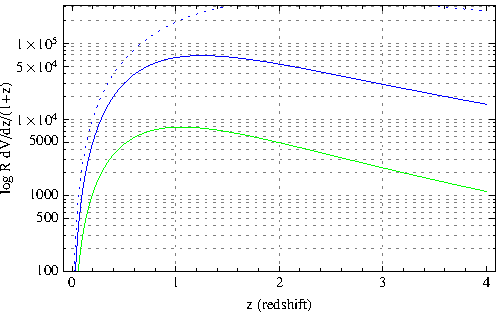
\includegraphics[angle=0,width=0.45\textwidth]{./Sec_ET_ScienceCase/visiondoc-EventRatePerRedshift}
%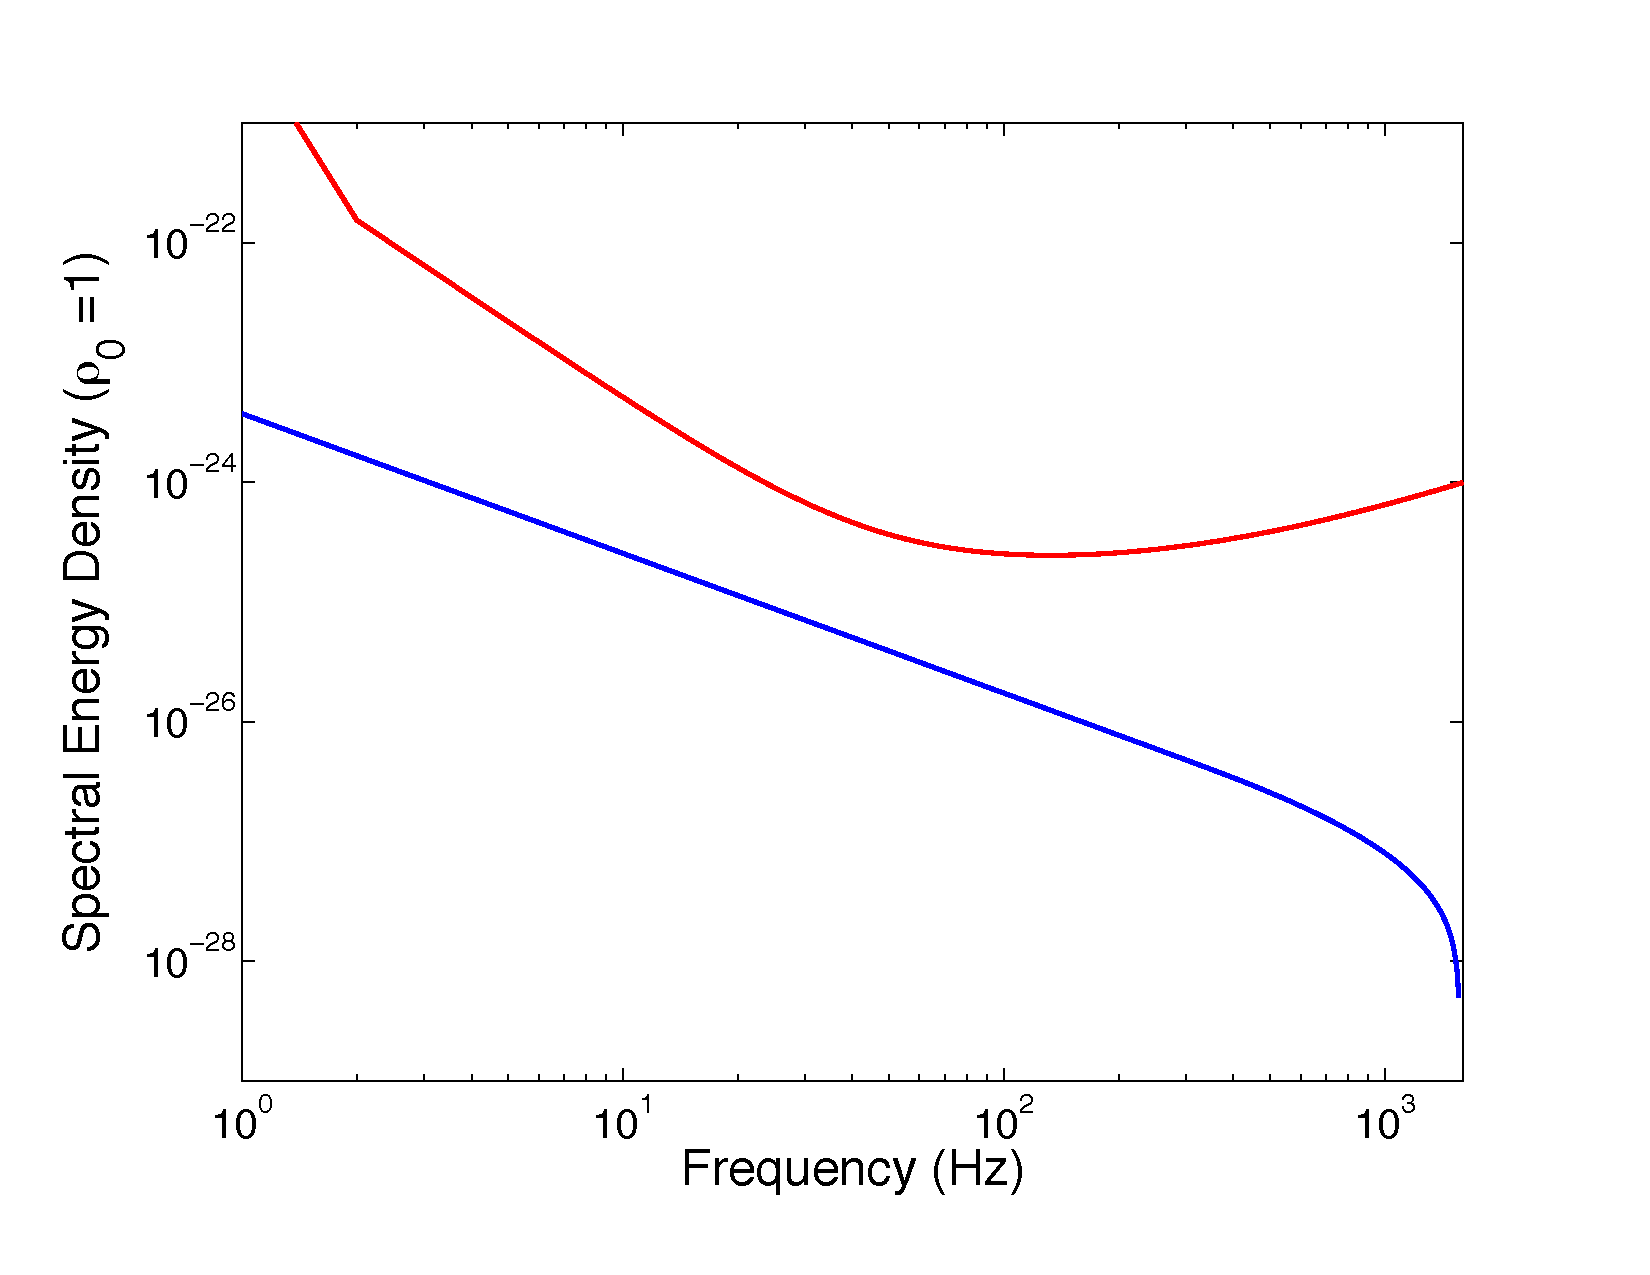
\includegraphics[angle=0,width=0.45\textwidth]{./Sec_ET_ScienceCase/BNS-Sh.pdf}
%\caption{
%Left: The merger rate $dR/dz$  on our past light cone versus  redshift.  Dotted blue 
%line extrapolates  the Milky Way double neutron star merger rate to the universe using
%Eq.~\ref{eq:TrivialMergerEstimate}, which assumes that merger rates trace the star 
%formation history~\cite{sfr-HopkinsBeacom2006} and that the Milky Way forms stars 
%at a rate $dM/dt_{MW}\simeq \dot{\rho}_{MW}/n_{mw} = 3 M_\odot$ yr$^{-1}$.   
%More detailed calculations that account for the finite delay between binary 
%birth and merger are shown in the two sold lines for   NS-NS (blue) and BH-NS (green) 
%binaries.   These delays insure ET will probe the redshift region where most 
%binaries merge.  Right: Spectral energy density of the background produced by 
%the coalescence of double neutron stars, compared to the sensitivity of ET-B.
%\label{fig:DNS_Sh}}
%\end{figure*}

If the stellar binary fraction in a globular cluster is sufficiently high,
two or more IMBHs can form \cite{Fregeau:2006}.  These IMBHs
then sink to the center in a few million years, where they form a binary
and merge via three-body interactions with cluster stars followed
by gravitational radiation reaction \cite{Fregeau:2006,AmaroSeoane:2007aw}. 
Then ET could detect $2000 \left(\frac{g}{0.1}\right) \left(\frac{g_{\rm cl}}{0.1}\right)$ 
mergers per year, where $g$ is the fraction of all globular clusters
hosting pairs of IMBHs, and $g_{\rm cl}$ is the fraction of star forming
clusters.  Mergers between pairs of globular
clusters containing IMBHs can increase this rate by up to a factor of
$\sim 2$ \cite{AmaroSeoaneSantamaria:2009}.
\FloatBarrier
%% \subsubsection{Measurement accuracies}
% \ledby{Van Den Broeck}

\FloatBarrier
\subsubsection{Continuous wave sources}
% \ledby{Krishnan}

Continuous wave sources that are discussed in this section are so-named because
these sources last for at least a few weeks, but typically for months or years, and 
produce signals with roughly constant amplitude and frequency varing relatively 
slowly over the observation time.  Such signals are expected to be
produced by rapidly rotating non-axisymmetric NSs which are
either isolated or in binary systems. A description of the 
signal emitted by such sources is given in Box \ref{box:cw}. There are 
a number of mechanisms which may cause the star to 
emit GWs.  These include deformations of the
NS crust, precession, magnetic fields, and internal oscillation
modes of the NS fluid.  
%([IAN] I dont think more detail is needed in the last sentence, maybe some references though)

%
\paragraph{Isolated neutron stars}

There are at present almost 2000 pulsars known from either radio or
X-ray observations. The parameters of many of these systems, i.e.\  the
sky location and frequency evolution, have been accurately measured. 
In this case we talk of \emph{targeted searches} for known NSs.
We assume the GW phase evolution to be tightly correlated with the
rotational phase as inferred from electromagnetic observations.  For
GW emission due to a non-negligible ellipticity, the
GW emission occurs at twice the rotational frequency of the star.
These two assumptions constrain the expected gravitational waveform
up to an unknown initial phase $\phi_0$, amplitudes $A_{+,\times}$ and
polarization angle $\psi$.  Methods have been developed to search over these
unknown parameters \cite{Jaranowski:1998qm} and to either measure the
amplitude $h_0$, or in the case that no signals are detected, to set
upper limits on it. The main issue in the analysis is how to compensate 
accurately for the Doppler shift due to the source-detector relative 
motion (and other relativistic effects), and the intrinsic spin-down of the source.

The benchmark for these searches is the indirect upper bound on $h_0$ set by
assuming that all of the kinetic energy of the star lost in the
spin-down is channeled into gravitational radiation as illustrated in Appendix 
\ref{box:sdl}. 
This assumption is not expected to hold for any of
the known pulsars where electromagnetic braking explains most of the
spin-down.  Nevertheless, the spin-down limit is still a very useful
benchmark for identifying astrophysically relevant targets and quantifying
search results. Setting an upper limit below the spin-down limit constrains
the fraction of spin-down energy that is emitted as GWs.

Initial interferometers have now set upper limits on a number of known 
pulsars using data from the LIGO, GEO and Virgo detectors
\cite{Abbott:2004ig,Abbott:2007ce, Abbott:2008fx}.  One highlight from
these results is beating the spin-down limit for the Crab pulsar
\cite{Abbott:2008fx} where the GW luminosity is
constrained to be less than $2\%$ of the spin-down luminosity
\cite{Collaboration:2009rfa}. ET will be able to detect continuous waves
from Crab even if it emits one millionth of the spin-down luminosity
in GWs.


\longetbox{i}{box:cw}
{Continuous Gravitational Waves}
{In the case of continuous waves, the waveforms for the two polarizations 
are given by
%
\begin{equation}
  \label{eq:2}
  h_+(t) = A_+\cos\Phi(t), \qquad  h_\times(t) = A_\times\sin\Phi(t),
\end{equation}
%
where $t$ is the time in the frame of the moving, accelerating
detector and $\Phi(t)$ is the phase of the GW; the 
amplitudes $A_{+,\times}$ depend on the other pulsar parameters, 
such as its rotational frequency, moments of inertia, the orientation of 
its rotation axis and its distance from Earth. The phase $\Phi$ takes 
its simplest form when the time coordinate used is $\tau$, the proper 
time in the rest frame of the NS:
%
\begin{equation}
  \label{eq:3}
  \Phi(\tau) = \phi_0 + 2\pi \sum_{n=0}^{s}
  \frac{f_{(n)}}{(n+1)!} \tau^{n+1}.
\end{equation}
%
Here $\phi_0$, $f_{(0)}$ and $f_{(n)}$ ($n\geq 1$)
are respectively the phase, instantaneous frequency and the spin-down
parameters in the rest frame of the star at the fiducial start time
$\tau=0$, $s$ is the number of spin-down parameters included in
the model, and $\iota$ denotes the angle between the line-of-sight to the
star and its rotation axis. It is useful to write the amplitudes
$A_{+,\times}$ in terms of a single number $h_0$
\begin{equation}
  \label{eq:1}
  A_+ = \frac{1}{2}h_0(1+\cos^2\iota) \,,\qquad A_\times = h_0\cos\iota\,.
\end{equation}
The exact expression of the overall amplitude $h_0$ depends on the specific mechanism producing the continuous signal. For instance, in the case of a tri-axial NS rotating with frequency $f_{rot}$ around a principal axis of inertia we have
\begin{equation}
h_0=\frac{4\pi^2G}{c^4}\frac{I_{zz}\epsilon f^2}{d},
\end{equation}
where $I_{zz}$ is the star's moment of inertia with respect to the rotation axis, 
the equatorial ellipticity $\epsilon$ is defined in terms of pricipal axis 
of inertia as $\epsilon=\frac{I_{xx}-I_{yy}}{I_{zz}}$, $d$ is the distance 
to the star and $f=2f_{rot}$ is the signal frequency.
\\[5pt]
The maximum expected signal frequency is below 2\,kHz. Potentially 
interesting sources are within the Galaxy, thus the distance $d\simeq 10$\,kpc. 
The standard value of the moment of inertia is $I= 10^{38}$\,kg\,m$^2$, 
although values in the range $(1-3)\times 10^{38}$\,kg\,m$^2$ are 
considered plausible. The typical values of ellipticity are largely 
unknown; the maximum value allowed by standard equations of state for 
NS matter is $\sim 5\times 10^{-6}$. Some exotic 
equations of state imply maximum values even two orders of magnitude 
larger.
}

The minimum signal amplitude detectable by a given targeted search depends 
directly on the detector sensitivity and scales with the square root of the observation time, as discussed in Appendix \ref{box:h0min}.  

It is informative to compare detectable values of $h_{0,\rm min}$ with the spin-down
limits for a number of known pulsars.
Figure~\ref{fig-CW-known} shows the detectable amplitude for Initial and
Advanced LIGO, Virgo and ET, and the spin-down limits for various known
pulsars. It is clear that the better low-frequency sensitivity of ET-D allows it to
reach the spin-down rate of almost all pulsars with spin frequencies
greater than 3\,Hz (corresponding to a GW frequency of 6\,Hz).
\begin{figure*}
\centering
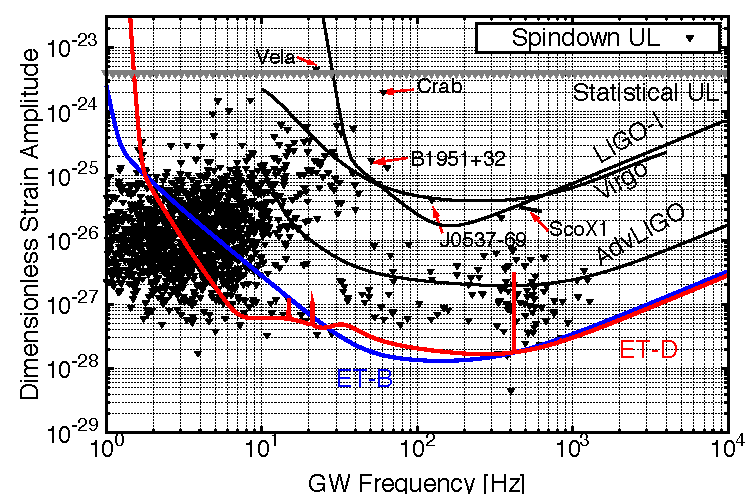
\includegraphics[angle=0,width=0.65\columnwidth]{./Sec_ET_ScienceCase/TheBigPicture_ETBD_5y.pdf}
\vskip 0.3cm
%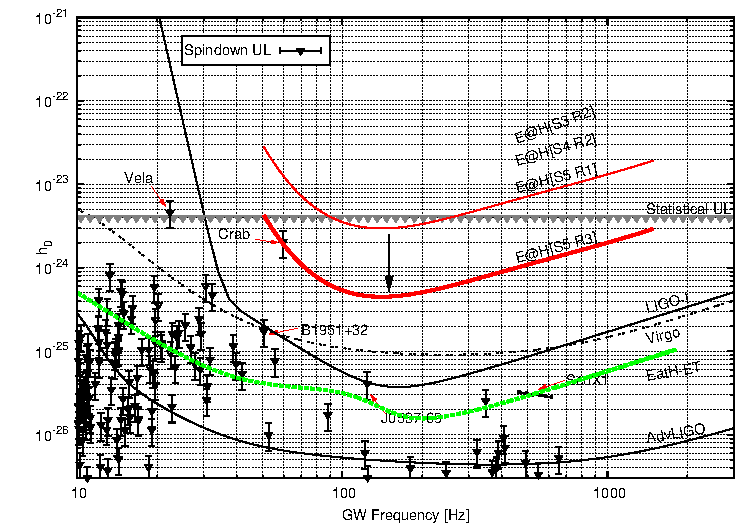
\includegraphics[angle=0,width=0.45\columnwidth]{./Sec_ET_ScienceCase/CW_unknownpulsars}
\caption{
Upper limits and spin-down limits for known pulsars. 
The detector sensitivity curves plot the minimum detectable amplitude 
of the GW averaged over sky positions and pulsar orientations. A detection
threshold based on a false alarm rate of 1\% and a false dismissal rate of 
10\% is assumed.  The spin-down limits assume the NS to have a moment of
inertia in the range 1-3$\times 10^{38}\,\textrm{kg\,m}^2$ and a $\pm
10\%$ uncertainty in its distance.  
% The spindown limit shown in the figure is the average of the upper limits 
% obtained by folding in these uncertainties.  
Initial LIGO and Virgo curves assume an integration time of 2 years while
the rest assume 5 years.  Initial LIGO consists of the H1, L1 and H2
detectors, Virgo is a single detector, aLIGO, ET-B and
ET-D are assumed to consist of three detectors. ET-D's better
sensitivity, compared to ET-B, at frequencies below 20\,Hz 
helps target a number of known pulsars.}
\label{fig-CW-known}
\end{figure*}

Let us turn now to the \emph{wide parameter space searches}. Here, instead of
targeting a known pulsar, the aim is to search for unknown sources in as large 
a portion of the parameter space (sky location, frequency, frequency derivatives) 
as possible.  Potential GW sources could be invisible in the EM band, either
because their radio pulses are not beamed towards us or because their
EM emission is dim due to having a very low magnetic field.
Such searches are computationally limited because the
number of templates increases much faster than linearly with the
observation time $T_{\rm obs}$.  The large number of templates affects the
search sensitivity in three basic ways. The first and most obvious one
is simply the discreteness of the template grid: SNR is lost by searching
for a GW signal with a template that does not exactly match. Secondly, it
leads to a large number of statistical trials, which increases the
false alarm rate and thus leads to a larger 
%effective 
SNR threshold for detection.
Finally, and most importantly, it limits the largest observation time
that can be considered; even given the increase in computer power
following Moore's law, this limitation will most likely still apply in the ET
era.

The problem of computational cost is addressed by the so-called
\emph{semi-coherent} methods. These rely on breaking up the full data
set into shorter segments of duration $T_{\rm coh}$, analyzing the segments coherently and
combining the power from the different segments incoherently. There
are a number of different techniques available for performing the
incoherent combination. %% **cites**.
For these searches, the sensitivity, incorporating all the effects mentioned 
above, is proportional to the square root of the total observation time and 
is given by Eq.~(\ref{hmin_blind}), Appendix \ref{box:h0min}. Typically, the output of a wide-area search 
is a set of \emph{candidates}, i.e.\ points in the source parameter space with 
values of a given statistic above a threshold. These candidates are then 
analyzed in a deeper way \emph{e.g.}\ by making coincidences with another set 
of candidates coming from a different dataset, followed by a full coherent 
analysis on the surviving candidates, in order to confirm or reject them.

%Let us now compare the prospects of detection with two proposed ET 
%sensitivity curves, ET-B and ET-D.
\begin{figure*}
\centering
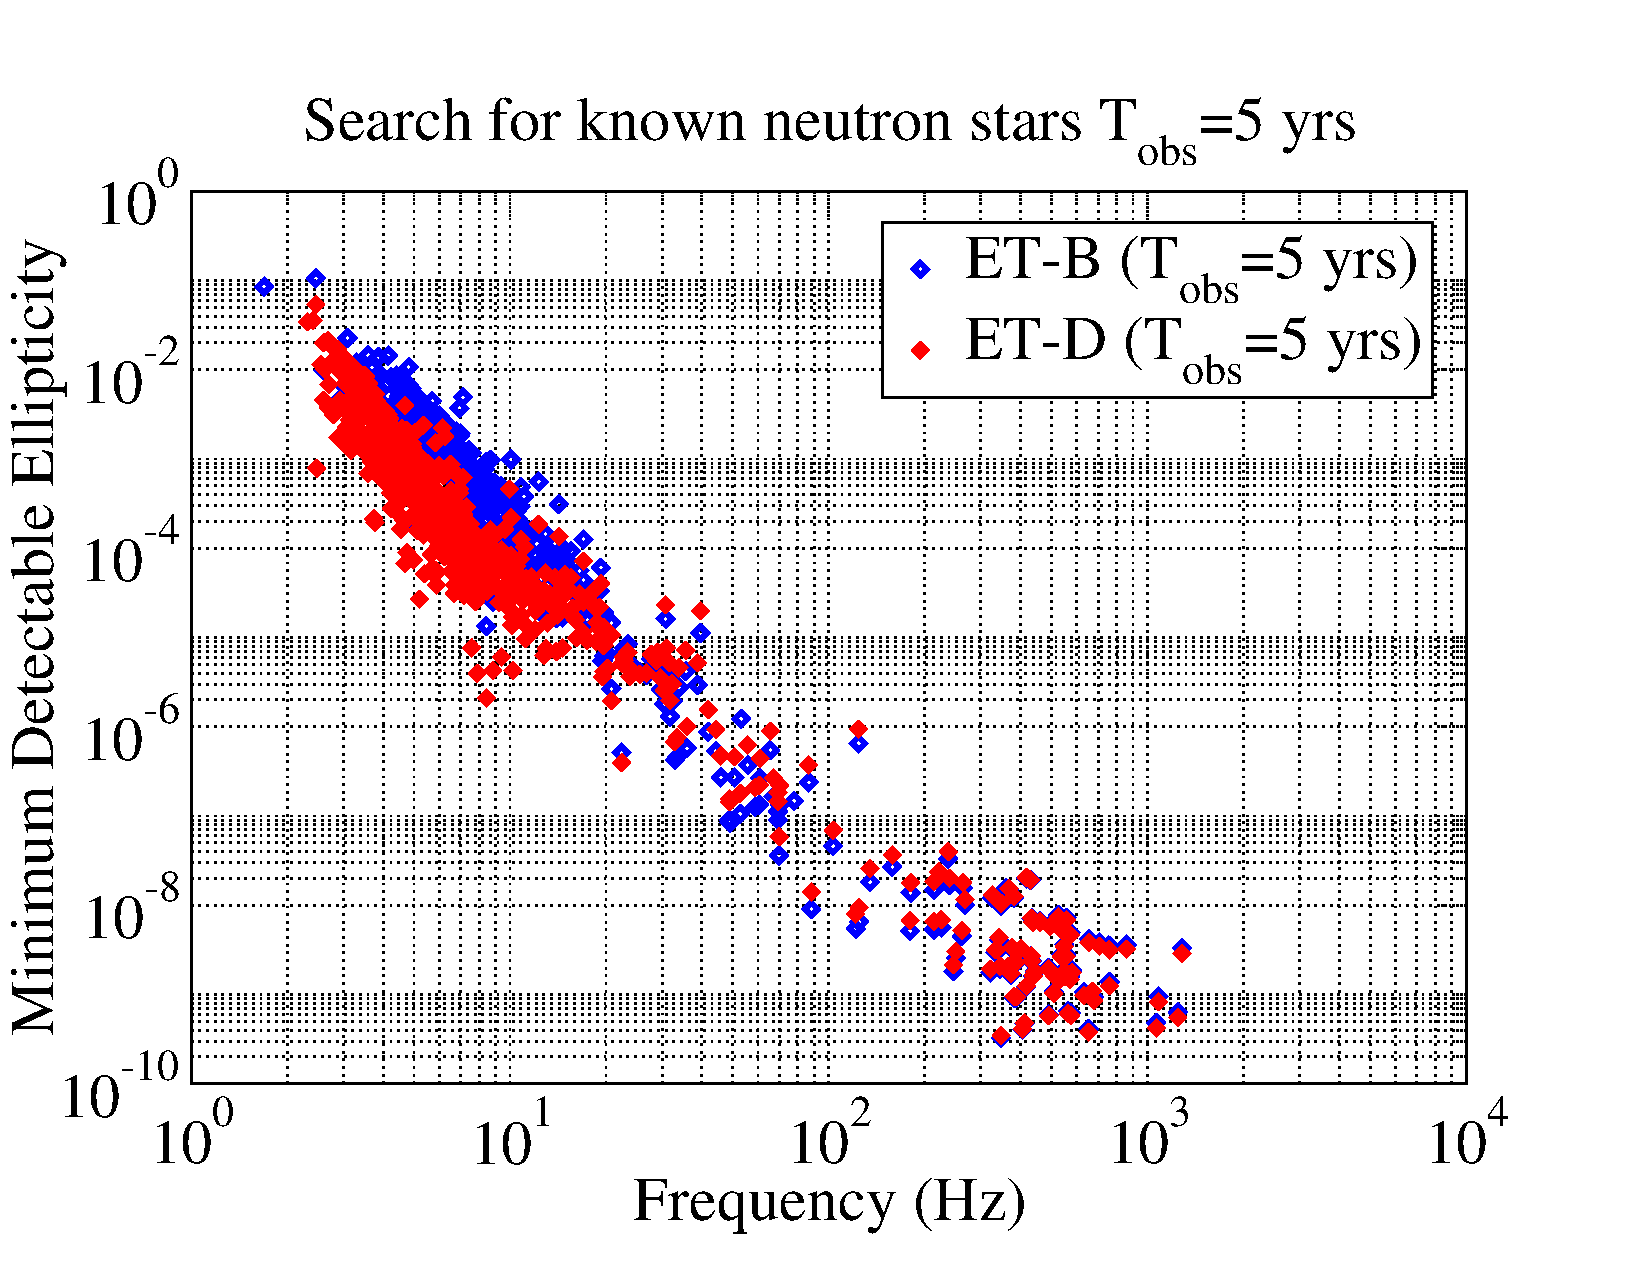
\includegraphics[width=0.49\textwidth]{./Sec_ET_ScienceCase/known_pulsars_ET_epsilon}
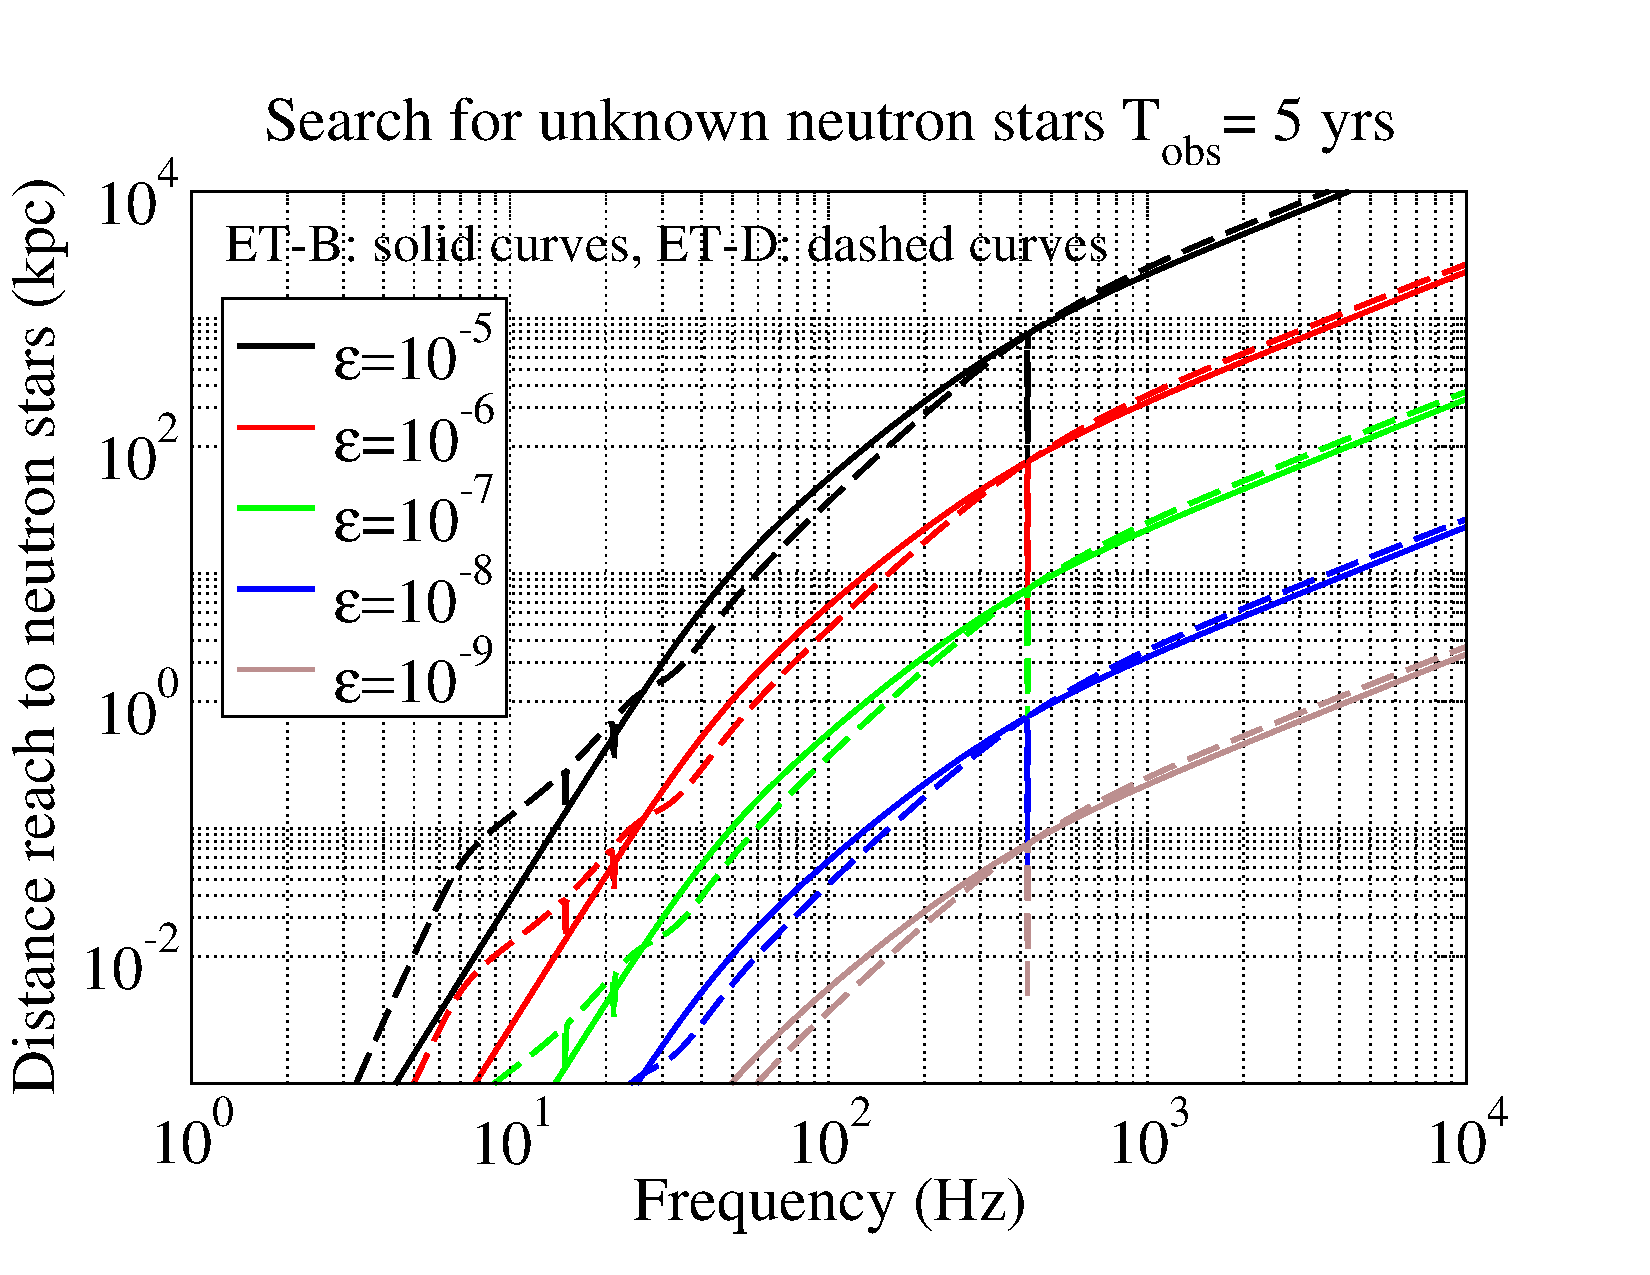
\includegraphics[width=0.49\textwidth]{./Sec_ET_ScienceCase/blind_rmax_ET}
\caption{Left: Minimum detectable ellipticity for known pulsars for 
ET-B and ET-D sensitivities. The search parameters are the same as 
for Fig.~\ref{fig-CW-known}. Right: Maximum distance of an unknown 
source in order to be selected among the candidates of an all-sky 
search with ET-B and ET-D sensitivities. Search parameters are given in the text.}
\label{sensi_knownpulsar}
\end{figure*}
\paragraph{Comparing prospects of detection for ET-B and ET-D sensitivities}
ET-B has a better sensitivity at extremely low frequencies, below $\sim 2$~Hz. 
ET-D, on the other hand, has a better sensitivity in the low frequency range, 
say between $2$\,Hz and $20$\,Hz. At intermediate frequencies, between 
$\sim 30$\,Hz and $\sim 300$\,Hz, ET-B has a slightly better sensitivity. 
The sensitivities of the two configurations are basically the same in the 
high frequency range.  Fig.~\ref{fig-CW-known} plots the minimum detectable
amplitude, assuming ET-B sensitivity (continuous blue line) and ET-D sensitivity 
(dashed red line), with an observation time
$T_{\rm obs}=5\,$yr, a false alarm probability of $1\%$ and a false dismissal
probability of $10\%$ (see Eq.~(\ref{hmin})), versus the spin-down limit of
the known pulsars taken from the ATNF Catalogue at
{\tt http://www.atnf.csiro.au/research/pulsar/psrcat/}. For comparison, the
upper limit reached by Initial and Advanced LIGO and Virgo are also shown but
assuming an integration time of 2 yrs for all except Advanced LIGO, for
which an integration time of 5 yrs is assumed.

We note that no pulsar has yet been found that could emit a
detectable signal with frequency below $\sim 2.5\,$Hz. Thus there
is no gain in having a good sensitivity at extremely low frequencies. On the
other hand, having a better sensitivity around $10\,$Hz impacts positively on
the possibility of detecting a continuous GW signal.

This can be seen also in Fig.~\ref{sensi_knownpulsar}, left panel, where the
ellipticity corresponding to the minimum detectable amplitude is plotted but
only for those pulsars for which the spin-down limit can be beaten in
an observation time of $T_{\rm obs}=5$\,yr. Not only is the number of pulsars for which
the spin-down limit can be beaten far larger for ET-D
but, more importantly, the minimum ellipticity needed to produce a detectable
signal is almost one order of magnitude lower in the $10\,$Hz range.
For instance, with ET-B we typically need $\epsilon$ in the
range $(0.1-5)\times 10^{-4}$ for pulsars emitting around $10\,$Hz, while $\epsilon
\sim (0.1-5)\times 10^{-5}$ is enough with ET-D. There are just a couple of pulsars
at frequencies below $\sim 3\,$Hz for which the spin-down limit could be
beaten with ET-B, but not with ET-D, with corresponding ellipticity in the
$10^{-2}$ range, a value difficult to reach even assuming an exotic equation
of state for NS matter. 

We must, however, keep in mind that the number of pulsars increases with decreasing 
frequency, and so also the probability that
extremely deformed, EM-dim, NSs exist, provided such large
deformations are attainable in nature.
At high frequency, in contrast, there is no relevant difference 
between the two detector configurations and fast spinning pulsars with 
ellipticity less than $\sim5 \times 10^{-8}$ could be detected.

Next, we consider the \emph{blind} search for unknown NSs. In 
this case we plot in Fig.~\ref{sensi_knownpulsar}, right panel, the maximum distance of a 
source to be selected among the candidates of an all-sky, semi-coherent search,
for different values of the NS ellipticity. An
observation time $T_{\rm obs}=5$\,yr and a coherent length 
$T_{\rm coh}=24$\,hr are assumed. Moreover,
the threshold for the selection of candidates is chosen in order to have
$10^9$ candidates.

In practice, we do not expect detections for signal frequencies below
$\sim 10\,$Hz for $\epsilon<10^{-5}$ (the
corresponding $r_{max}$ becomes unrealistically small). And also
considering extremely deformed NSs ($\epsilon> 10^{-5}$)
signal frequencies below $\sim 3\,$Hz are basically excluded. Then, having
a better sensitivity at very low frequencies gives basically no gain. On the
other hand, having a better sensitivity around $10\,$Hz somewhat increases
the possibility of detection: for instance, assuming
$\epsilon=10^{-5}$, the maximum
distance that a search can reach, goes from $\sim 10\,$pc with ET-B to
$\sim 80\,$pc with ET-D at $8\,$Hz, while it goes from $\sim
30\,$pc to $\sim 150\,$pc at $10\,$Hz. On the contrary, in the range 
$\sim 30-100$\,Hz with ET-B the distance reach is about a factor of 2 greater. 

These conclusions do not significantly change assuming a
longer coherent step (compatible with the computing power believed to be
available in the ET era), because the sensitivity increases only as
$T_{\rm coh}^{1/4}$, see Eq.~(\ref{hmin_blind}), Appendix \ref{box:h0min}.

%Observations of accreting neutron stars lead to perhaps the most
%important reason why, irrespective of the mechanism at work, at least
%some neutron stars might be emitting detectable gravitational
%waves.  

%% Spin frequency measurement plays an important role in what follows
%% and, as we shall see, can \cite{Watts2008}

%This is the observation that even the fastest accreting
%neutron stars spin at rates much lower than the expected break-up
%frequency.  The current record is 716\,Hz, %% **cite**,
%while the
%theoretically expected upper limit is more than 1\,kHz. %% **cites**.
%Following a suggestion by Bildsten \cite{Bildsten:1998ey}, it is
%possible that this limit occurs because of the balance between the
%spin-up torque due to the accreting matter, and the spin-down torque
%due to GW emission.  A short calculation assuming a
%link between the observed X-ray luminosity with the accretion rate,
%and taking the mountain scenario for the emission mechanism leads to
%the following estimate of the GW amplitude:
%\begin{equation}
  %\label{eq:6}
  %h_0 = 3 \times 10^{-27}F_{-8}^{1/2}\left(\frac{R}{\rm 10
        %km}\right)^{3/4}\left(\frac{1.4 M_\odot}{M}\right)^{1/4}
  %\left(\frac{{\rm 1~kHz}}{\nu_s}\right)^{1/2}.
%\end{equation}
%This is seen to be depend on frequency: $h_0 \propto \nu_s^{-1/2}$.

\FloatBarrier

\subsubsection{Burst sources}
Many transient astronomical phenomena, such as supernovae, gamma-ray
bursts and glitching pulsars, could produce bursts of gravitational 
waves that last for as short as a few milliseconds (\emph{e.g.}\ supernovae)
to several minutes or longer (\emph{e.g.}\ certain instabilities of NSs, 
discussed below). Detecting such waves, especially in coincidence with optical, 
X-ray, gamma-ray radiation or neutrinos could help resolve decades-old 
problems in astronomy. Gravitational waves will be a very powerful 
addition to multi-messenger astronomy (see~\cite{springerlink:10.1007/s10714-010-1019-z} for a review),  allowing a view into the dark and 
dense cores of sources that are inaccessible to other windows of 
observation.

\paragraph{Gravitational wave bursts from gravitational collapse}
Neutron stars and BHs are formed from the gravitational collapse 
of a highly evolved star or the core collapse of an accreting white
dwarf.  In either case, if the collapse is non-spherical, perhaps induced by
strong rotation or magnetic field, then GWs could 
carry away some of the binding energy and angular momentum, depending 
on the geometry of the collapse. 
Gravitational collapse events are the progenitors of supernovae of 
various types.  Supernovae of Type II are believed to occur at a rate of between 
0.01 and 0.1 per year in a Milky Way equivalent galaxy; thus, within 5\,Mpc,
we might expect an event rate of about 1 per 2 years \cite{ando:05}. 

Simulating gravitational collapse is a very active area of numerical 
astrophysics. Most simulations also predict the energy and spectral 
characteristics of the emitted GWs~\cite{ott:09,Living:Fryer}. 
However, it is still beyond the capabilities of computers to simulate a 
gravitational collapse event with all the physics that might be necessary 
to give reliable predictions: three-dimensional hydrodynamics, neutrino 
transport, realistic nuclear physics, magnetic fields, rotation. In fact, 
it is still by no means clear why Type II supernovae explode at all: simulations 
typically have great difficulty reversing the inflow and producing an explosion
with the observed light-curves and energetics. It may be that the answer lies 
in some of the physics that has to be oversimplified in order to be used in 
current simulations, or in some neutrino physics that we do not yet know.

In a typical supernova, simulations suggest that GWs might extract 
between about $10^{-11}$ and $10^{-7}$ of the total available
mass-energy~\cite{dimmelmeier:08,murphy:09,marek:09b,scheidegger:10b}, and the
waves could come off in a burst whose frequency might lie in the range
of $\sim 200$\,--1000\,Hz.
Using representative values for a supernova in our galaxy, lying at $D=10$\,kpc, 
emitting the energy equivalent of $E=10^{-8}\,M_\odot$ at a frequency of $f=1$\,kHz, 
and lasting for $T=2$\,ms, the observed amplitude would be (cf. \ref{eq:amplitude})
%
\begin{equation}
h \sim 1.5 \times 10^{-21}
\left ( \frac{E}{10^{-7}\,M_\odot} \right )^{1/2}
\left ( \frac{1\mathrm{\,ms}}{T} \right )^{1/2}
\left ( \frac{1\mathrm{\,kHz}}{f} \right )
\left ( \frac{10\mathrm{\,kpc}}{D} \right ).
\label {eq:amplitudeB}
\end{equation}
%
This amplitude is large enough for current ground-based detectors to observe with a
reasonably high confidence, but of course the event rate within 10\,kpc is
expected to be far too small to make an early detection likely. ET can
detect an amplitude that is two orders of magnitude smaller or from a distance
of 1\,Mpc. ET might, therefore, see a supernova collapse once per four or six years.

\begin{figure*}
\begin{center}
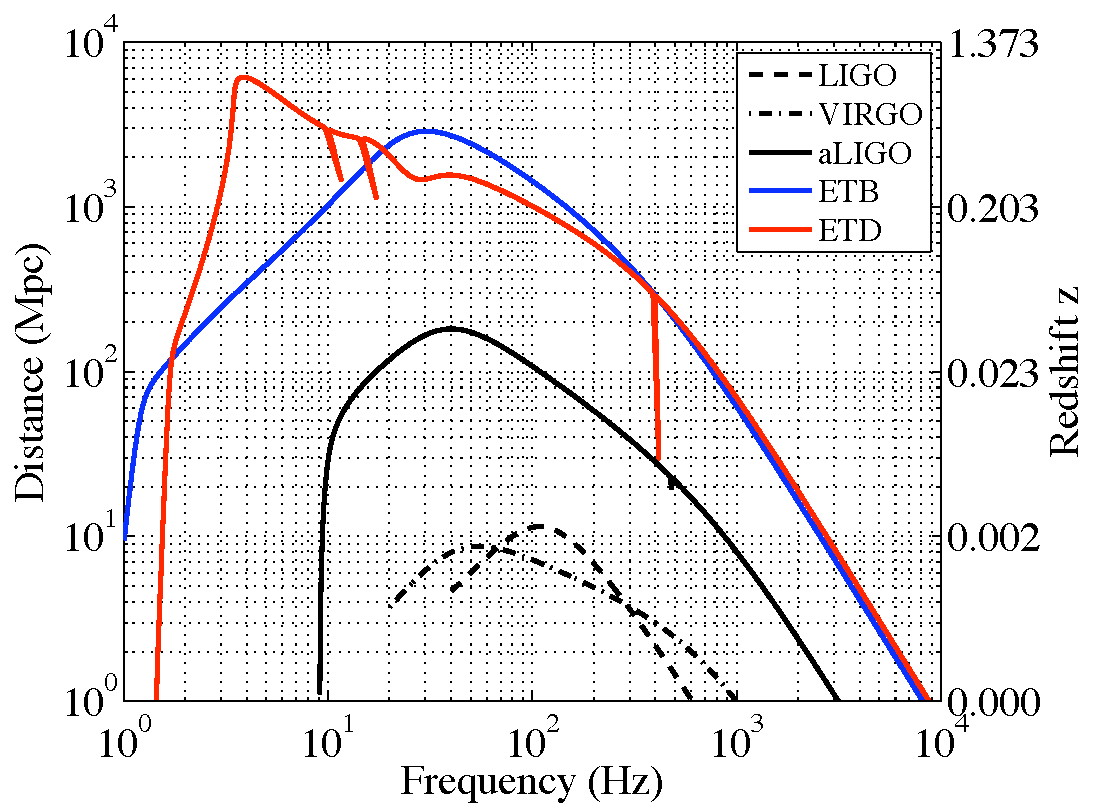
\includegraphics[width=0.60\textwidth]{./Sec_ET_ScienceCase/GWB_distance.pdf}
\caption{90\%-confidence lower limit on distance for GRB burst sources assuming 
a GRB energy emission of $E^{\rm iso}_{\rm GW} = 0.05\,M_{\odot} c^2 \sim 9 \times 10^{52} 
{\rm ergs}$. A redshift correction of $(1+z)$ has been used in computing the lower limit.
\label{fig:distanceFreq_5percentMsol}}
\end{center}
\end{figure*}

\paragraph{Gamma-ray bursts}
There is increasing evidence that gravitational collapse also produces
some of the observed gamma-ray bursts~\cite{Hjorth2003} 
in \emph{hypernovae} and \emph{collapsars}~\cite{Woosley1993, MacFadyenWoosley1999}.
As we shall discuss in more detail, several different classes of GRBs are now known
although their cause is not yet completely understood. There are no
reliable GW emission models from collapsars or hypernovae although some 
estimates give as large as $10^{-2}M_\odot$ for isotropic GW emission for
GRB progenitors.  BNS and NSBH mergers (the likely progenitors of 
most short GRBs) will have isotropic-equivalent emission on the order 
of ($0.01$-$0.1$) $M_\odot$ in the 100 to 200 Hz band. For long GRBs, 
fragmentation of the accretion disk \cite{davies:2002,king:2005,piro:07}
could produce inspiral-like chirps with $(0.001$-$0.01)\,M_\odot$ emission 
in GW.  The suspended accretion model \cite{vanPutten:grb} also
predicts an energy emission of up to $(0.01$-$0.1) M_\odot$ in this
band.


A GRB at a distance of $D=4.2\,\rm Gpc$ (a redshift of $z\simeq 0.7$) 
emitting the energy equivalent of $E=5\times 10^{-2}\,M_\odot$ 
at a frequency of $f=1$\,kHz, and lasting for $T=1$\,ms, produces an amplitude of~\cite{springerlink:10.1007/s10714-010-1019-z}
%
\begin{equation}
h \sim 10^{-23}
\left ( \frac{E}{5\times 10^{-2}\,M_\odot} \right )^{1/2}
\left ( \frac{1\mathrm{\,ms}}{T} \right )^{1/2}
\left ( \frac{1\mathrm{\,kHz}}{f} \right )
\left ( \frac{4.2 \mathrm{\,Gpc}}{D} \right ),
\label {eq:amplitudeC}
\end{equation}
%
Figure \ref{fig:distanceFreq_5percentMsol} shows the distance 
reach of Initial and Advanced LIGO, Virgo and two possible noise curves considered
for ET (ET-B and ET-D)
to such a GRB. The waveform emitted in the process is not known with any certainty
and so the distance reach is calculated by assuming that GW bursts are detected
by search algorithms that look for excess energy in a time-frequency map.
While aLIGO might detect rare closeby GRBs, ET could probe GRBs at cosmological
distances, assuming GWs extract about $0.05\, M_\odot$ in the process.


\paragraph{Pulsar glitches and magnetar flares}
Neutron stars have a rich spectrum of non-radial normal modes, which 
which can be classified according to key key restoring force that 
affects the fluid motion. In the context of GW astrophysics f-, g-, p-, w-, 
and r-modes have all been studied~\cite{AnderssonKokkotas1998,Andersson:2003}.  
Just as in the case of BHs, these normal modes are a superposition of 
damped sinusoids, but in the NS case the frequencies and damping times 
depend on the complex physics of NS interiors.  Modelling the NS oscillation 
spectrum requires physics beyond what is within reach for laboratory 
experiments. This sets a severe challenge, but at the same time it is a key 
reason why the problem is important. It also provides ample motivation for 
attempts to provide observations that can be used to test various theoretical 
models, e.g. concerning the state of matter at extreme densities. A promising, 
at least in principle, strategy follows the very successful asteroseismology 
programme for normal stars. In the case of the sun, the matching of inferred 
non-radial oscillation modes to theoretical predictions has led to a much 
improved understanding of the interior conditions. Similarly, one may expect 
that GW observations of oscillating NSs may place useful constraints both 
on bulk parameters like mass and radius, and hence the overall EoS, and 
detailed physics, like internal composition gradients.  In fact, even 
knowing accurately the frequency and decay time of just the fundamental 
$\ell=2$ f-mode would be enough to eliminate most currently considered 
equations of state~\cite{AnderssonKokkotas1998}.

The f-modes of NSs are promising emitters of GWs that may be excited 
by glitches or by the nuclear explosions on accreting neutron stars that 
are thought to produce X-ray flares and soft gamma-ray repeater events. 
The rise-time of X-ray emission can be as short as a few 
milliseconds\,\cite{2008Kes75}, which might be impulsive enough to excite 
acoustic vibrations. If the rise time of the explosion matches the period 
of the mode well enough, then a substantial fraction 
of the energy released could go into mechanical vibrations, and almost all of this 
fraction would be carried away by GWs, since other mode-damping mechanisms 
inside NSs tend to be less efficient. 

The viability of these scenarios is difficult to quantify, given our general 
lack of understanding of the detailed dynamics associated with them. 
Presently, most available models are based on back-of-the-envelope 
phenomenology. This is well illustrated by the radio-pulsar glitches, 
enigmatic spin-up events seen in (mainly) relatively young NSs like Crab and Vela. 
It is easy to estimate that these events are associated with energies of 
order $ 10^{42}$~erg ($10^{-12}\,M_\odot$). This sets a useful benchmark 
energy level for discussion of GW events associated with NS in our galaxy, 
but it obviously does not constitute a real estimate of the energy 
released as GWs.  Nevertheless, assuming this level of energy emission 
through the f-mode at 2~kHz of a star at a distance of 10~kpc it is easy 
to estimate that these events could create a wave of effective amplitude 
(see Eq.\,\ref{eq:amplitudeB}) around $10^{-23}$. (The effective amplitude 
assumes we can do matched filtering, which in this case is not very 
difficult.) This kind of amplitude should be well within the reach of ET.  
Observations of these modes would immediately constrain the cold-matter 
nuclear EoS in significant ways~\cite{AnderssonKokkotas1998, Living:AnderssonComer}.

It is also important to note that NS events seen in X-rays and gamma rays 
can be much more energetic.  In fact, NS oscillations may have already been 
observed in X-rays~\cite{WattsStrohmayer2007}. Quasiperiodic oscillations 
seen in the tails of strongly magnetised NS (magnetar) flares agree well 
with predicted crustal modes, whose restoring force is the shear strength 
of the crust. These observations mainly probe  the physics of the crust, 
which represents the low-density region and is not expected to leave a 
strong imprint on emitted GWs. Nevertheless, the observations 
allows us to test the astero-seismology paradigm \cite{Samuelsson:2007}, 
an exercise that has placed (weak) constraints on the EoS. As far as GW 
astrophysics is concerned, a key question concerns to what extent the 
more massive NS core takes part in these event. The general expectation 
is that the magnetic field provides an efficient coupling 
between the crust and the core. The upshot of this could be that the 
magnetar events are predominantly due to the interior magnetic dynamics, 
which may make them associated with detectable GWs. Establishing this 
requires better theory modelling, but it is still clear that ET will 
be able to place useful constraints on any such mechanism.


\paragraph{Relativistic instabilities of compact stars} The most 
promising scenarios for detectable NS oscillations involve some 
kind of instability. Realistic NS may become unstable during 
different evolutionary stages. A rapidly and differentially rotating 
proto-NS may be dynamically unstable due to the so-called bar-mode 
(the l=m=2 f-mode). At less extreme differential rotation, the 
so-called low T/W instability may operate. Proto-NSs may also be 
convectively unstable, leading to growing g-modes, due to temperature 
gradients. The mechanisms connect the birth of a NS with the 
supernova event, and the level of excitation of the involved 
oscillations depends to a large extent on how the core-collapse 
proceeds. Another class of instabilities is powered by with the 
emission of GWs. First demonstrated by Chandrasekhar~\cite{ChandraCFS} 
in 1971, this instability was shown to be generic in rotating stars 
by  Friedman and Schutz~\cite{Friedman1978}  a few years later. They 
proved that the unstable modes have a very simple signature depending 
on the pattern speed of the mode, i.e.\ the angular velocity at which 
the crests of the pattern passes about the rotation axis of the star. 
If this velocity is in the same sense as the rotation of the star, 
but slower than that of rotation, then the mode would be unstable in 
a perfect fluid star. This instability has come to be known as the 
CFS instability, after the three authors who discovered and explained 
it.  

The presence of an instability is, however, not sufficient to make 
the scenario astrophysically relevant. In order to play a role for 
real NSs, any instability must overcome a number of damping mechanisms. 
The problem then becomes exceedingly difficult, especially since we 
do not have very precise models for the various transport coefficients 
needed for a model of NS dissipation. Nevertheless, there has been 
considerable progress on this problem. Focussing on the instability 
associated with the f-mode, Lindblom and Detweiler~\cite{LINDBLOM1977} 
showed that the effect of viscosity runs counter to that of radiation 
reaction, so that the instability is strongest in modes with the 
longest wavelengths,  in principle the quadrupole modes. However, 
numerical calculations for Newtonian stellar models with realistic 
viscosity show~\cite{Lindblom:1995zs} that the f-modes are not vulnerable 
to the instability. This would weakens the impact for GW physics 
significantly. In addition to this, it has been demonstrated that the 
friction associated with superfluid vortices may suppress the 
instability entirely \cite{Lindblom:1995zs}.
These results do not, however, signal the demise of this mechanism. 
First of all, the instability is stronger in fully relativistic 
models~\cite{Stergioulas:1997ja}, especially since the $l=2$ mode 
may also be unstable.  Secondly, the superfluid friction becomes 
relevant only after the star has cooled below the relevant transition 
temperature (below $10^9$~K). Hence, there may still be room for the 
f-mode instability to play a relevant role in very young NSs. Moreover, 
as the f-mode is an ideal GW emitter (with a short instability growth 
time, and possible large nonlinear amplitude) the associated signals 
may well be within reach with ET even for extragalactic sources. This 
is an interesting possibility that need to be explored by more detailed 
modelling. 

Most recent activity on NS instabilities has concerned a different 
class of oscillations, namely the Rossby, or r-modes. In contrast 
to the f-modes, which become unstable above a critical rotation rate, 
these modes are unstable in a rotating perfect fluid star at all 
rotation rates. The associated GWs comes from the current-multipoles, 
rather than from the mass multipoles as in the case of the f-mode. 
This makes the modelling different, but the main physics issues 
remain the same. Investigations by a number of authors~\cite{Lindblom:1998wf, 
Andersson1999, Owen1999} have shown that the r-mode instability could 
be relevant in hot, rapidly-rotating stars.  In particular, it may 
lead to a nascent NS spinning down significantly, losing angular 
momentum as GWs.  The instability might also operate in mature, 
accreting NSs, such as those in low mass X-ray binaries (LMXB) 
(see the next section). 

In principle, the fact that the r-mode instability window depends on 
a balance between GW driving and various dissipation mechanisms makes 
it a sensitive probe of NS core physics.  Observations allow us to 
test our understanding of exotic physics associated with 
hyperons~\cite{LindblomOwen2002, Lackey2006}. , deconfined quarks and 
large scale superfluids/superconductors \cite{Living:AnderssonComer}. 
The signal associated with various r-mode scenarios should be 
detectable with ET for systems within, and possibly beyond, our 
galaxy \cite{Bondarescu:2009}
but in order to facilitate such detections we need to make progress 
on thorny theory issues. Key issues concern the interaction with 
magnetic fields in the star, the damping due to the vortex mediated 
mutual friction in a superfluid , the possible role of turbulence, 
the boundary layer at the crust-core interface and exotic bulk viscosity 
due to the presence of hyperons or deconfined quarks in the deep 
neutron star core. These problems are all very challenging. In addition, 
we need to  model the GW signal from an unstable r-mode. This is also 
difficult because, even though the r-mode growth phase is adequately 
described by linear theory, nonlinear effects soon become important 
leading to the evolution, and the  associated GW signal, becoming 
very complex.  Future ET observations have the potential to test 
various proposed r-mode scenarios, improving our understanding of 
extreme NS physics significantly.   


\FloatBarrier
\subsubsection{Stochastic background} \label{source_stochastic}
The superposition of a large number of unresolved sources of GWs 
produces a stochastic background.  We can distinguish between two 
contributions: a primordial background of cosmological origin, a 
memory of the early stages of the Universe, and a background of 
astrophysical origin, a memory of the evolution of the galaxies 
and star formation. We summarize basic properties of a stochastic 
GW background in Box~\ref{box:stoch_basics}. The strength of the
background is characterized by the dimensionless quantity
$\Omega_{\rm GW}(f),$ which is the ratio of the energy density
in GWs to the critical density of the Universe as a function
of frequency. 

\paragraph{Primordial background}
The essential interest of a primordial GW background is the prospect 
of probing the behaviour of matter and the evolution of the Universe 
at very high energy scales and densities---potentially even above the 
energies achievable at current particle colliders. This is feasible 
thanks to the very large redshift factor (well over ten orders of 
magnitude) appropriate to times before primordial nucleosynthesis: 
waves created at extremely short length scales may now be accessible 
to terrestrial detectors. At such short distance scales and high 
energies, evidence for new physics may emerge, such as particles 
beyond the Standard Model, high-temperature phase transitions and 
topological defects, inflation and reheating, or even extra spatial 
dimensions.  

\etbox{i}{box:stoch_basics}{The Spectrum of Stochastic GW Background}
{
It is usual to characterize the intensity of a random field of 
GWs by its energy density as a function of 
frequency.   Since the energy density of a plane wave is the same 
as its flux (when $c=1$), we have from Eq.\,(\ref{eq:flux})
$\rho_{\text{GW}} = \pi f^2h^2/4.$
But the wave field in this case is a random variable, so we must replace $h^2$ 
by a statistical mean square amplitude per unit frequency 
(Fourier transform power per unit frequency) called $S_{\mathrm{GW}}(f)$, 
so that the energy density \emph{per unit frequency} 
is proportional to $f^2 S_{\mathrm{GW}}(f)$.  It is then conventional to talk about the 
energy density per unit logarithm of the frequency, which means multiplying by $f$.    
The result, after being careful about averaging over all directions of the 
waves and all independent polarization components, is~\cite{Allen:1997ad, Thorne1987}
\begin{equation}
\frac{{\rm d}\rho_{\text{GW}}}{{\rm d}\ln f} = 4\pi^2 f^3 S_{\mathrm{GW}}(f).
\end{equation}
What is of most interest is the energy density as a fraction of the 
closure or critical cosmological density, given by the Hubble constant 
$H_0$ as $\rho_c = 3H_0^2/8\pi$.  The resulting ratio is called $\Omega_{\text{GW}}(f)$:
\begin{equation}
\Omega_{\text{GW}}(f) = \frac{10\pi^2}{3H_0^2}f^3S_{\mathrm{GW}}(f).
\label{eq:stochastic}
\end{equation}
%\\[5pt]
%For a stochastic background of astrophysical origin:
%\begin{equation}
%\Omega_{\rm gw}(\nu_o)=5.7 \times 10^{-56}  \nu_o \int_{z_{\min}}^{z_{\max}} \frac{\dot{\rho}^o(z)}{(1+z)E(z)}\frac{dE_{\rm gw}}{d\nu}(\nu_o)dz
%\end{equation}
%where $\dot{\rho}^o(z)$ is the number of events in an element of comoving volume and interval of time in the observer frame, $\frac{dE_{\rm gw}}{d\nu}$ the typical spectral energy density of a single source and $E(z)$ a function that depends on the cosmology. 
%\\[5pt]
To evaluate the contributions of various sources to the background we 
take a fiducial value $H_0=70$\,km\,s$^{-1}$\,Mpc$^{-1}$ for the Hubble 
parameter and assume a flat Universe with $\Omega_\Lambda = 0.7$.
}

\begin{figure*}
\centering
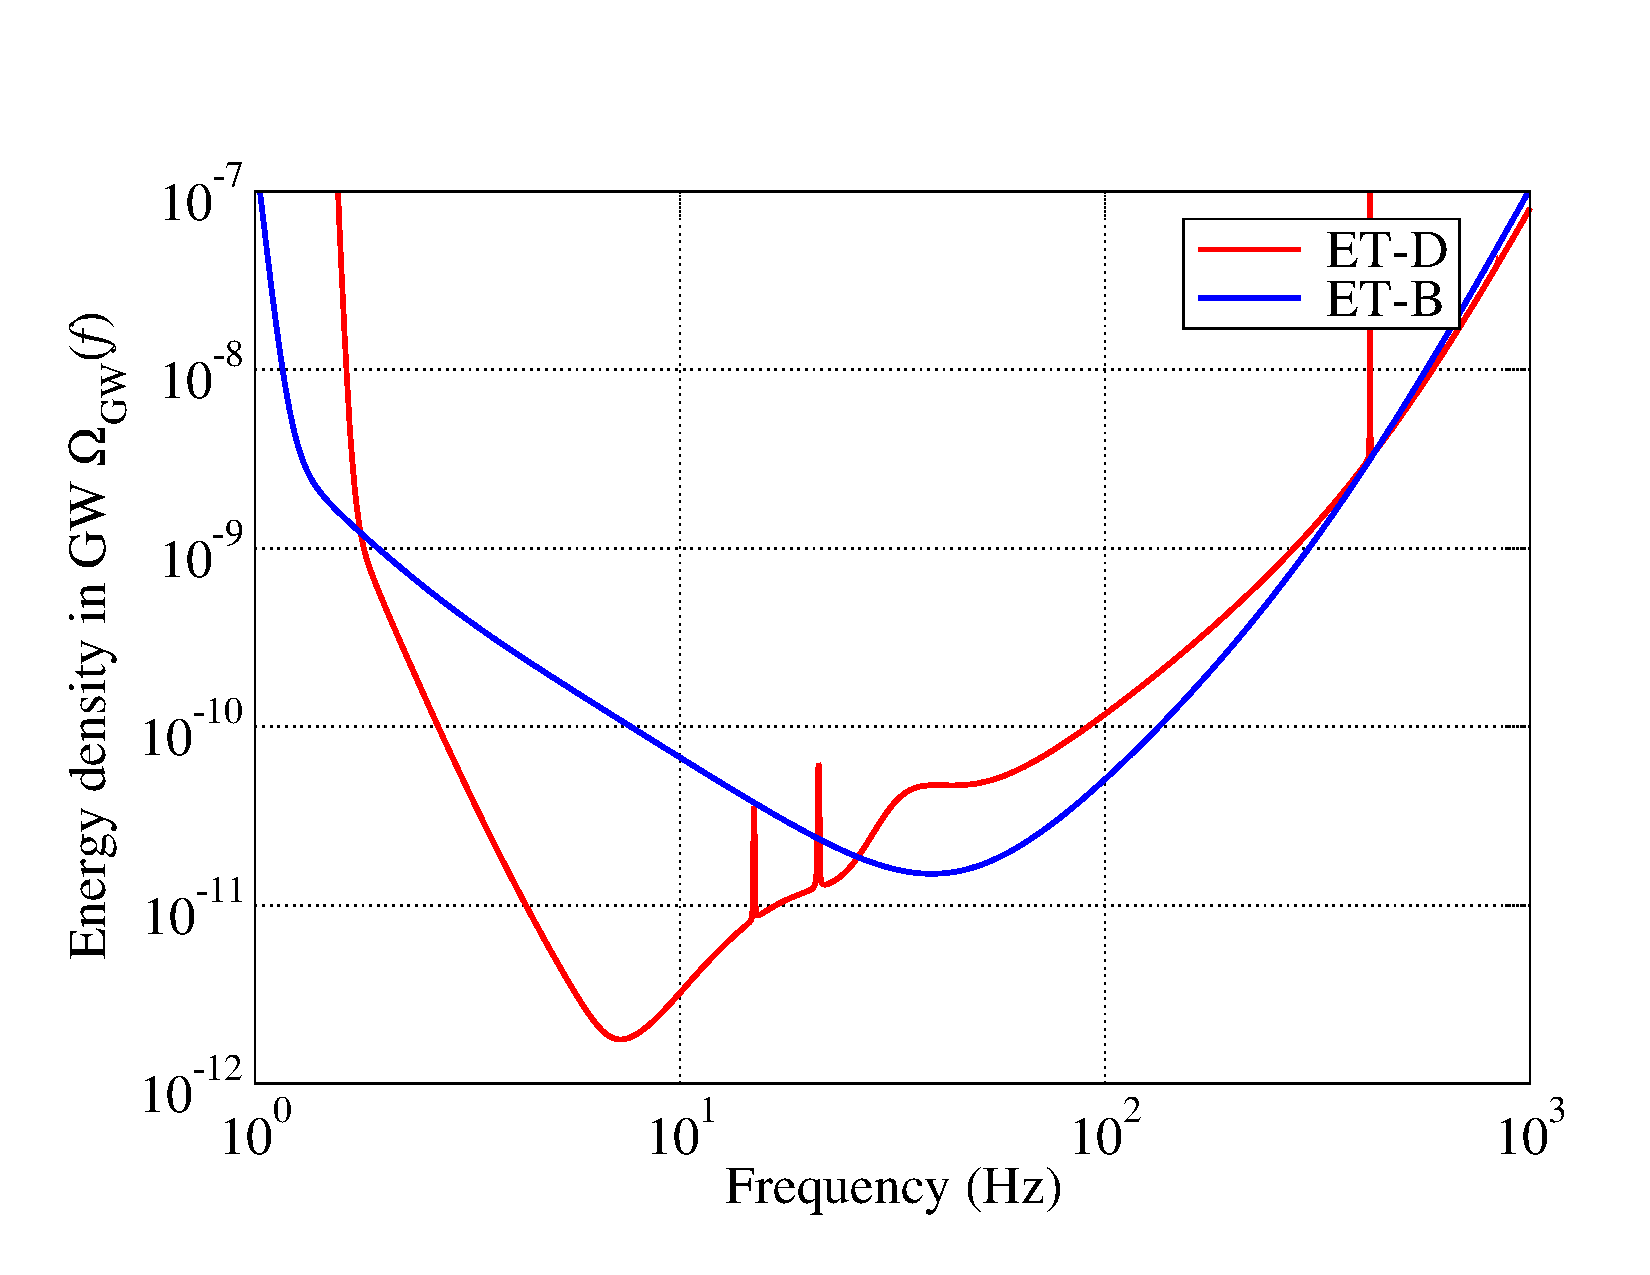
\includegraphics[width=0.60\textwidth]{./Sec_ET_ScienceCase/GWB.pdf}
\caption{The sensitivity ET-B and ET-D detectors to
stochastic background of GW. The curves show the energy density in GW that 
ET would be sensitive to after a year's integration at 95\% 
confidence level.}
\label{fig:stochastic}
\end{figure*}

The ultimate goal of detector development is the observation
of the background radiation from the Big Bang. It is expected to be very weak, 
but it will come to us unhindered from as early as $10^{-30}$~s, and it could 
illuminate the nature of the laws of physics at energies far higher than we 
can hope to reach in the laboratory. 

\paragraph{Astrophysical background}
The astrophysical contribution is important for at least two reasons.
On the one hand, it may mask the cosmological background in some 
frequency windows;  on the other hand, its detection would put 
strong constraints on the physical properties of compact objects 
and their evolution with redshift, such as the mass of NSs or BHs, the 
ellipticity and the magnetic field of NSs or the rate of 
compact binaries.

What is particularly interesting is that using stochastic backgrounds, 
we are able to put constraints on the mean values and not on the 
properties of the brightest sources, more likely in the tail of the 
distributions. 



\paragraph{Detecting stochastic backgrounds}
Random radiation is indistinguishable from instrumental noise in a single 
detector, at least for short observing times. If the random field is produced by
an anisotropically-distributed set of astrophysical sources (the binaries in our 
galaxy, for example) then over a year, as the detector changes its orientation, the 
noise from this background should rise and fall in a systematic way, allowing 
it to be identified. But this is a rather crude way of detecting the radiation, and 
a better way is to perform a cross-correlation between two detectors, if available. 

In cross-correlation, which amounts to multiplying the outputs and integrating, the 
random signal in one detector essentially acts as a template for the signal in the 
other detector. If they match, then there will be a stronger-than-expected correlation. 
Notice that they can only match well if the wavelength of the GWs is longer
than the separation between the detectors: otherwise time delays for waves reaching one 
detector before the other degrade the match. In this regard, ET's topology is 
particularly important. Since it hosts several detectors at the same location there
is no time delay involved and hence all frequencies contribute to the cross correlation.

The outcome of cross-correlation is not like standard 
matched filtering, however, since the ``filter'' of the first detector has as much 
noise superimposed on its template as the other detector. As a result, the 
amplitude SNR of the correlated field grows only with observing time as $T^{1/4}$, 
rather than the square root growth that characterizes matched filtering~\cite{Thorne1987};
sensitivity to $\Omega_{\rm GW},$ however, grows as $\sqrt{T}.$ 
\paragraph{ET's sensitivity to stochastic background}
The only tight constraint on  
$\Omega_{\text{GW}}$ from non-gravitational-wave astronomy is that it 
must be smaller than $10^{-5}$, in order not to disturb the agreement 
between the standard Big Bang model of nucleosynthesis (of helium and
other light elements) and observation. If the Universe contains
this much gravitational radiation today, then at the time of
nucleosynthesis the (blue-shifted) energy density of this radiation
would have been comparable to that of the photons and the three
neutrino species. Although the radiation would not have participated
in the nuclear reactions, its extra energy density would have required
that the expansion rate of the Universe at that time be
significantly faster, in order to evolve into the Universe we see
today. In turn, this faster expansion would have provided less time
for the nuclear reactions to ``freeze out'', altering the abundances
from the values that are observed today~\cite{Pagel:2000,Steigman:2007xt}. 

First-generation interferometers have already set direct limits 
\cite{Abbott:2009ws} on the cosmological background below the 
nucleosynthesis limit at $\Omega_{\rm GW} < 6.9\times 10^{-6}.$ 
Figure \ref{fig:stochastic} plots the sensitivity of Advanced LIGO
and ET to stochastic backgrounds assuming cross-correlation of data
over a period of one year. The plot is constructed using the formula 
(\ref{eq:stochastic}) taking $S_{\rm GW}=2.56\,S_h(f)/\sqrt{f\,T_{\rm yr}},$
where $S_h(f)$ is the noise power spectral density of the detector
in question, $T_{\rm yr}$ is the number of seconds in a year and a
factor of 2.56 is inserted to account for the SNR needed for a 95\%
confidence level.  Advanced detectors will probe stochastic backgrounds of strengths
$\Omega_{\rm GW} \sim 10^{-9}$ (see Fig.~\ref{fig:stochastic}) but
ET, thanks to its better low-frequency sensitivity, could detect
backgrounds at levels approaching $\Omega_{\rm GW} \sim 10^{-12}$ 
around frequencies of 10\,Hz. 

Sections \ref{cosmo_stochastic} and \ref{astro_stochastic}
discuss possible sources of stochastic backgrounds of primordial
and astrophysical origin and the physics we can
learn by detecting such backgrounds with ET.

\clearpage

\FloatBarrier
\subsection{Fundamental physics and strong field tests of GR}

The rich variety of sources and phenomena observed by
GW detectors can potentially be used
to address outstanding questions in fundamental physics.
The sources in question will be in dense environs
of ultra-strong gravity and will therefore provide a cosmic
laboratory for understanding phenomena and matter in
extreme conditions of density, temperature, and/or magnetic
fields. Moreover, BBH are
fundamentally geometric objects whose interaction close
to merger will provide insights into the nature of 
BH spacetimes and of gravity in ultra-strong fields.
Here we will discuss what fundamental physics
questions and strong-field tests of gravity could be
addressed by ET.

\FloatBarrier
\subsubsection{Polarization of gravitational waves}
In Einstein's theory of gravity, GWs have only two polarizations, 
the plus and cross polarizations discussed in Box \ref{box:gw}. 
In scalar-tensor theories GWs have four polarizations more 
than in GR. Observations of gravitational waves 
could exploit this difference to test GR.

In the long
wavelength approximation (i.e.\ when the wavelength is
much longer than the typical distance between test masses),
plus and cross polarizations cause quadrupolar deformations
in space and the proper distance between test masses changes
in a direction transverse to the propagation of the waves 
(see Fig.\,\ref{fig:pol}, Box \ref{box:gw}).  Other 
polarizations could cause motion of test masses longitudinal
to the direction of propagation as well as other patterns 
in the transverse plane. 

ET, with its three interferometers, will be able to resolve
the two polarizations, assuming that GR is the correct description
of gravity. With a network of other advanced or third generation
detectors that might be available at the time one could independently 
measure the polarization and check if the two measurements are
consistent with one another. Conclusively showing (to within 
experimental uncertainties) the absence of other polarizations 
could rule out a whole class of alternatives to GR. Advanced
detectors could do this to some extent but high SNR events that
ET is likely to see will provide compelling evidence.


\subsubsection{Bounding graviton mass}
% \ledby{Arun: June 8th}\\
In Einstein's theory, gravitational radiation travels at
the speed of light.  This means that gravitons, the particle
counterparts of GWs, are massless particles.
Although there is currently no strong motivation to
consider massive graviton theories from an experimental
point of view, they are natural extensions of Einstein's
theory.  In a massive graviton theory, GWs
would not travel at the speed of light and this can be
tested by observation of gravitational-wave sources
at very great distances.  To do so we would need a
source which emits both GW and EM radiation simultaneously.
By measuring the difference in their arrival times we could 
measure or constrain the speed of GWs.

Supernovae and BNS and NSBH systems are sources that are expected to 
exhibit after-glows in EM radiation soon after they emit a burst of GWs. 
If the source is near enough (a few Mpc in the case of supernovae, and
redshifts of a few in the case of coalescing binaries) and the
event is well-localized on the sky (fraction of a
degree depending on the distance to the source),
then it could be observed in coincidence as a transient
EM and GW event.

Current theories of supernovae and coalescing binaries
cannot accurately predict how promptly after the collapse
(in the case of SN) or merger (in the case of binaries)
EM radiation will follow. However, the expected delay is
no more than one second.
If GWs arrive a time $\Delta t$ after EM
waves, then the fractional difference in their speeds is
given by
\begin{equation}
\frac{|\Delta v|}{c} = 3.2 \times 10^{-18}
\left ( \frac{|\Delta t|}{1\,\rm s} \right )
\left ( \frac{3\, \rm Gpc} {D} \right )
\end{equation}
where we have assumed that the source is at a distance of
$D=3\,\rm Gpc$. This can be used to constrain the graviton
mass but there is a more robust method that could yield
better upper limits.

Gravitational waves in a massive graviton theory would suffer disperson and
the effect would be greater the farther an observer is from the source.
Thus, observations of inspiralling compact binaries at high redshifts
can be used to place better bounds on the mass of the graviton, or equivalently
the Compton wavelength of the graviton~\cite{bss:will.98}, than is possible
by comparing the arrival times of GW and EM radiation from a source. Moreover, 
bounds from GW dispersion do \emph{not} require the detection of an EM counterpart 
associated with the GW signal.
%
\begin{figure}[t]
\centering
%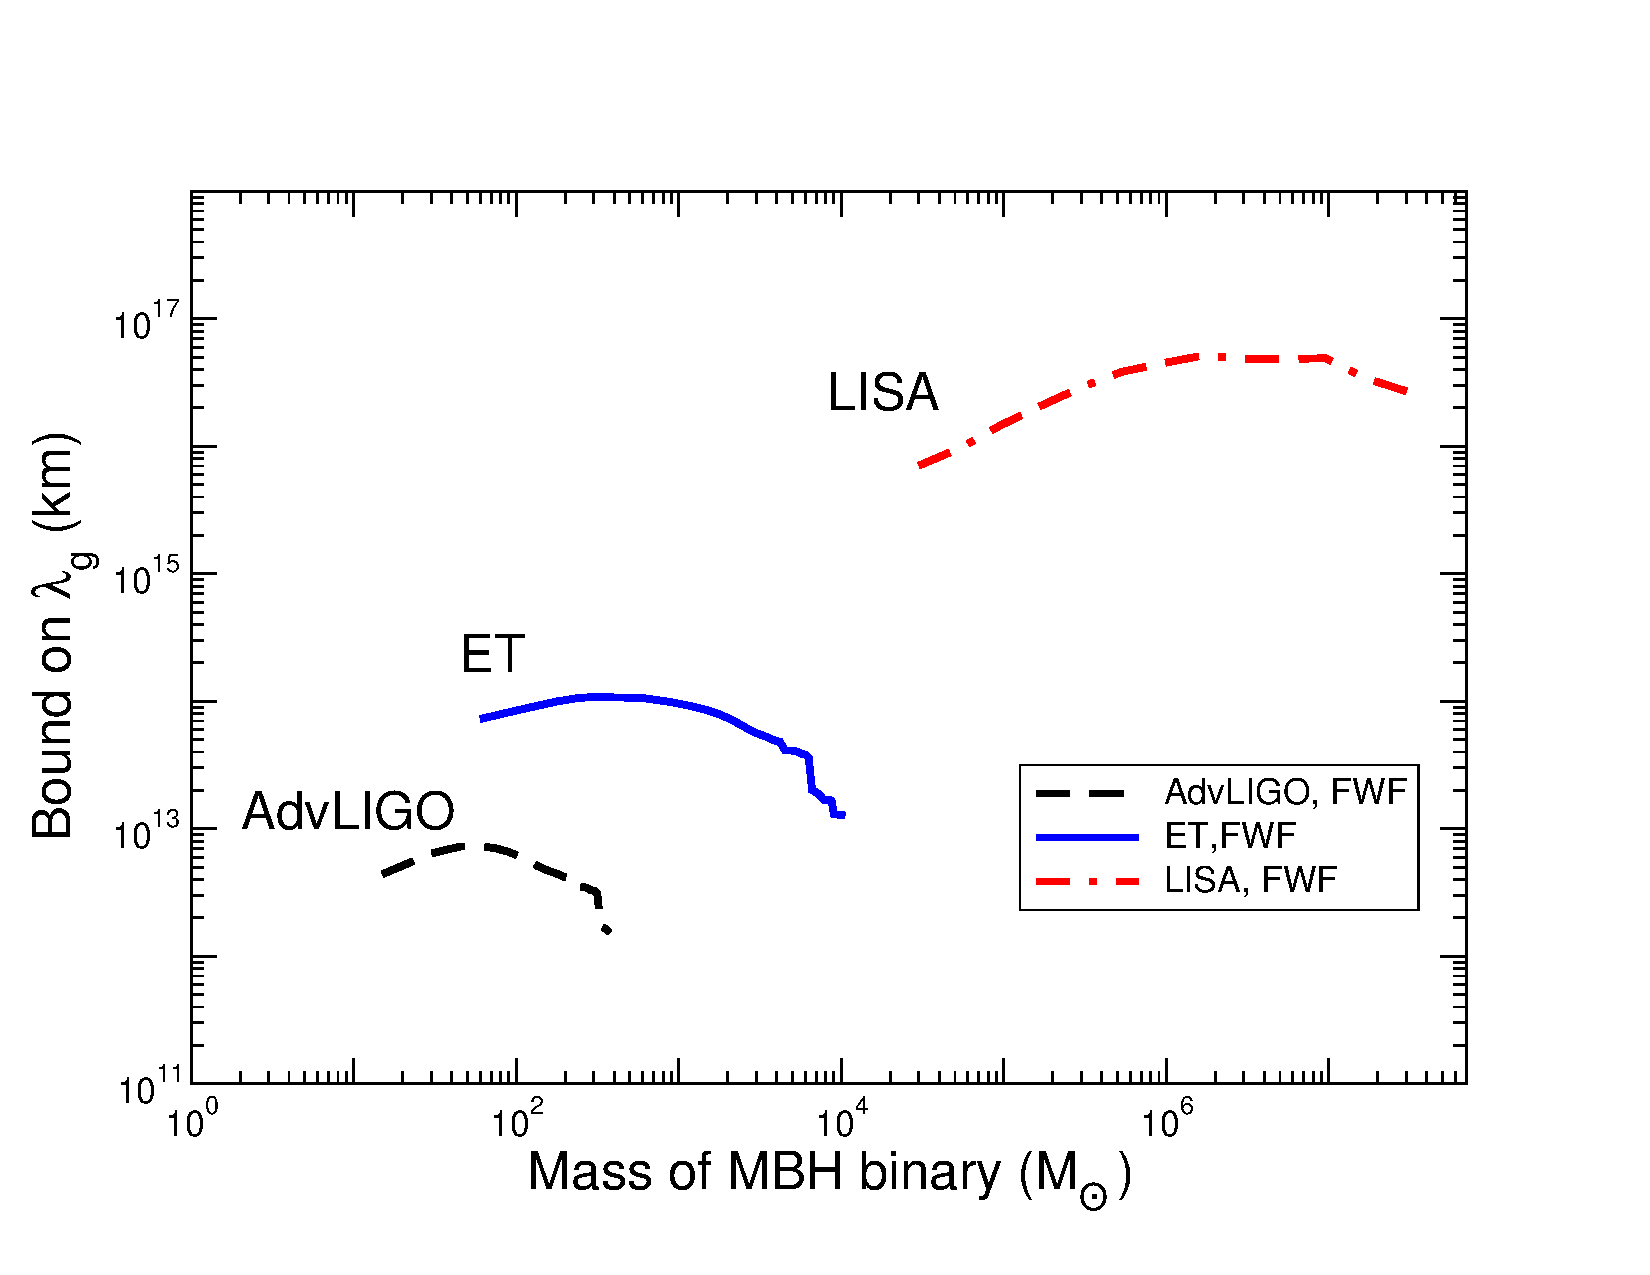
\includegraphics[scale=0.29]{./Sec_ET_ScienceCase/AdvLIGO-ET-LISA_MassiveGraviton.pdf}
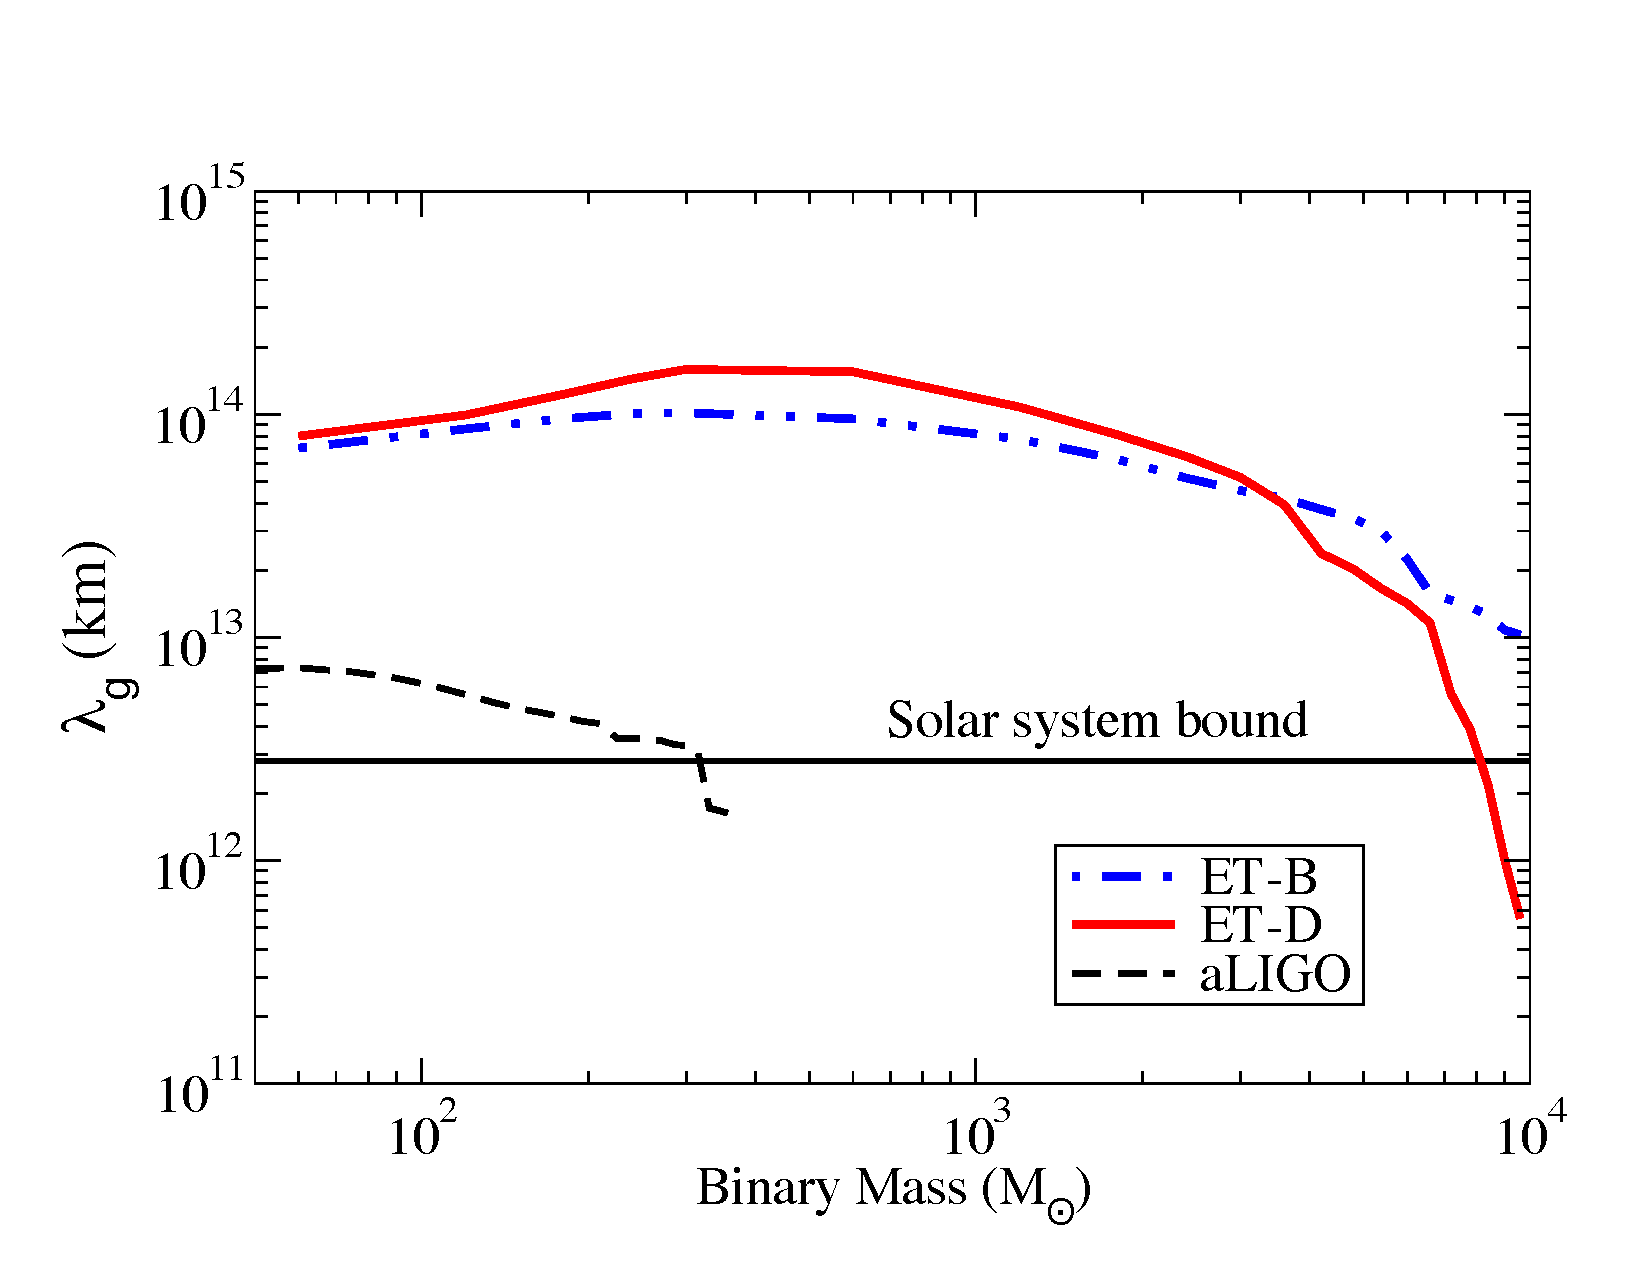
\includegraphics[width=0.49\textwidth]{./Sec_ET_ScienceCase/ET-BnD_MG_1Hz_Massratio2.pdf}
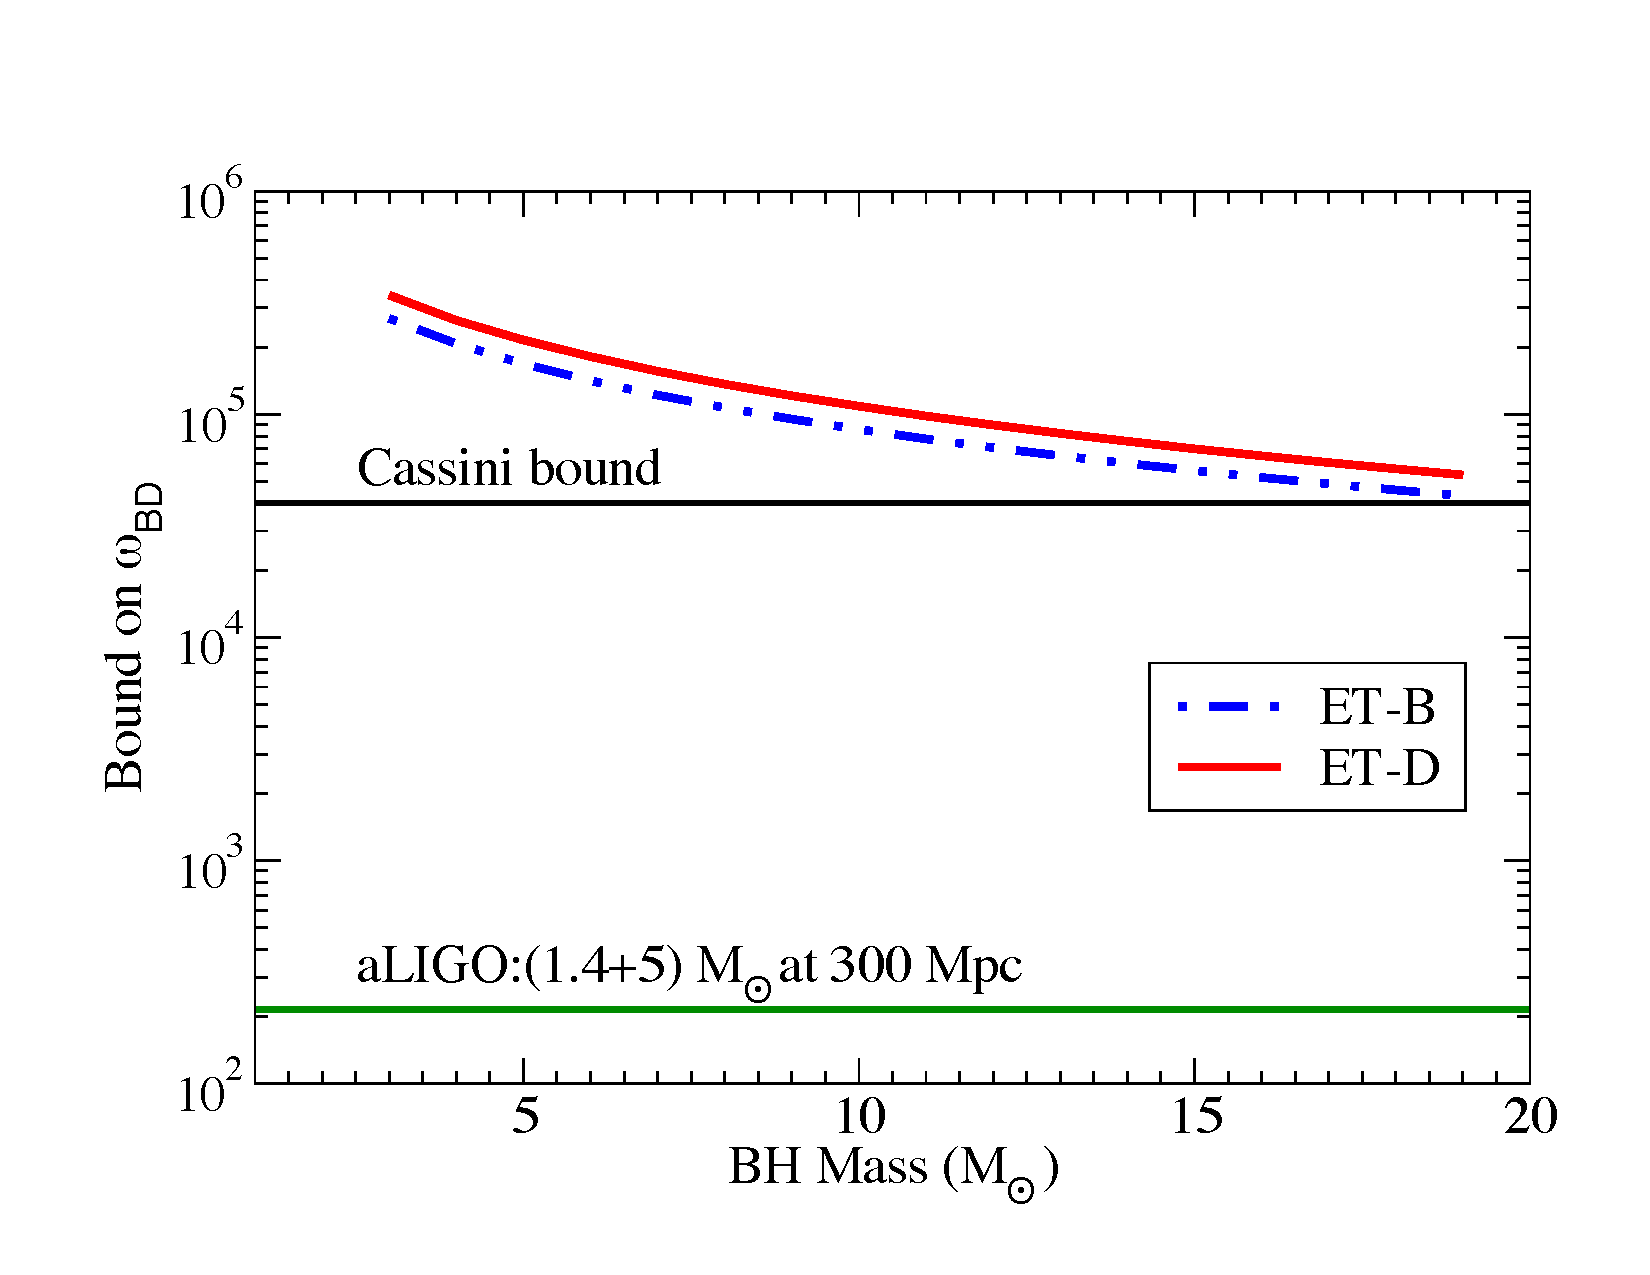
\includegraphics[width=0.49\textwidth]{./Sec_ET_ScienceCase/OmegaBD_1Hz_BH_Mass.pdf}
\caption{
\emph{Left panel:} Bounds on the graviton Compton wavelength that can be
deduced with ET-B and ET-D sensitivity curves as function of the 
total mass of the binary.  The mass ratio for all sources is taken to be 2.
ET can beat the current solar system bound by up to two orders of magnitude.
The limit is independent of the distance to the binary as long as the SNR is
large enough for the Fisher matrix calculation to be reliable. 
\emph{Right:} Bounds on the Brans-Dicke parameter ($\omega_{BD}$) as a function
of the total mass of the NSBH binary observed. For all systems, the NS mass 
is assumed to be 1.4\,$M_\odot.$  The existing bound from the Cassini 
experiment and the possible bounds from aLIGO are also shown.}
\label{fig:MassGravAll}
\end{figure}

The basic idea is simple: if there is a mass associated with the propagation 
of GWs (``a massive graviton''), then the speed of propagation $v_g$ will depend 
on the wavelength $\lambda$ as (in units $c=1$)
$v_g \approx 1 - (\lambda/\lambda_g)^2$, where 
$\lambda_g$ is the Compton wavelength of the graviton, in the limit where 
$\lambda \ll \lambda_g$.  Irrespective of the nature of the alternative 
theory that predicts a massive graviton, 
%(and notwithstanding the difficulties in defining such theories free of 
%pathologies such as the ZvDV discontinuity~\cite{Zakharov70,Veltman70})
it is reasonable to expect the differences between such a hypothetical theory 
and GR in the predictions for the evolution of compact 
binaries to be of order $(\lambda/\lambda_g)^2$. This quantity will be very 
small, given that close to merger $\lambda \sim 10^3$\,km for stellar mass 
BBH, BNS and NSBH inspirals and $\lsim 10^5$\,km for binary IMBH inspirals.

As a result, the gravitational waveform seen by an observer near to a
source will be very close to that predicted by GR.
However, as seen by a detector at a distance $D$, hundreds 
of Mpc away, the phasing of the signal will be distorted because of 
the shifted times-of-arrival, $\Delta t \sim D(\lambda/\lambda_g)^2,$ 
of the waves emitted with different wavelengths during the inspiral.   
In addition to measuring the astrophysical parameters of the system, 
such as masses and spins, the matched filtering technique permits one 
to estimate or bound such effects.

Bounds based on observations of BBH by ET have now been computed~\cite{AW09}. 
%The signal model comprises amplitude-corrected, general relativistic 
%waveforms which are 3PN accurate in amplitude~\cite{BIWW96,ABIQ04,BFIS08,Broeck2007}
%and 3.5PN accurate in phasing~\cite{Blanchet1995,BFIJ02,B96,BDEI04,DIS01,DIS02}.  
%The component stars are assumed to be non-spinning.
%Previous calculations used waveforms which are of Newtonian order in amplitude
%and 2PN order in phase.  As opposed to the Newtonian waveforms, the 3PN 
%amplitude-corrected waveforms contain eight harmonics of the oribtal phase
%$\Psi$ from $\Psi$ up to $8 \,\Psi$, the leading quadrupole component being 
%$2\Psi$.
%The effect of a massive graviton was included in the expression for the 
%orbital phase following Ref.~\cite{bss:will.98}.  
The wavelength-dependent 
propagation speed changes the arrival time $t_a$ of a wave of a given emitted 
frequency $f_e$ relative to that for a signal that propagates at the speed 
of light; that time is given, modulo constants, by
\begin{equation}
t_a = (1+z) \left [ t_e + \frac{D}{2\lambda_g^2 f_e^2} \right ] \,.
\label{time}
\end{equation}
Here $f_e$ and $t_e$ are, respectively, the wave frequency and time of 
emission as measured at the emitter; $z$ is the cosmological redshift, and
\begin{equation}
D \equiv \frac{(1+z)}{a_0}\int_{t_e}^{t_a} a(t) dt \,,
\label{D}
\end{equation}
where $a_0=a(t_a)$ is the present value of the scale factor\footnote{For 
$z\ll1$, $D$ is the same as the luminosity distance $D_{\rm L}$. Hence one 
can take $D\simeq D_{\rm L}$ in the case of ET for which sources considered 
are at 100 Mpc.}.  
%In the frequency domain, this adds a term to 
%the phase $\psi(f)$ of the Fourier transform of the waveform given by 
%$\Delta \psi(f) = -\pi D/f_e \lambda_g^2$.   Then, for each harmonic of the 
%waveform with index $k$, one adds the term
%\begin{equation}
%\Delta \psi_k (f) = \frac{k}{2} \Delta \psi(2f/k) = - \frac{k^2}{4} \pi  D/f_e \lambda_g^2 \,.
%\label{phaseterm}
%\end{equation}
%Here $k=2$ denotes the dominant quadrupole term, with phase $2\Psi$, $k=1$ denotes the term with phase $\Psi$, $k=3$ denotes the term with phase $3\Psi$, and so on.
%
This is an ad-hoc procedure
because a massive graviton theory will undoubtedly deviate from GR not 
just in the propagation of GW, but also in the way GW damping affects 
the phase and the amplitudes of the emitted radiation.  
% If, for example, such a theory introduces a leading correction to the 
% quadrupole phasing $\psi_{\rm quad} \sim (\pi {\cal M} f_e)^{-5/3}$ of 
% order $(\lambda/\lambda_g)^2 \times (\pi {\cal M} f_e)^{-5/3}$, where 
% $\cal M$ is the chirp mass, then the propagation induced phasing term 
% (\ref{phaseterm}) will be larger than this correction term by a factor 
% of order $k^2 (D/{\cal M})(\pi {\cal M} f_e)^{8/3} \sim (D/{\cal M})v^8$.  
% Since $v \sim 0.1$ for the important part of the binary inspiral, and 
% $D \sim$ hundreds of Mpc. 
However, it turns out that hundreds of Mpc away from the source,
the propagation effect will dominate over wave generation effects \cite{AW09}.  
In any case, given the fact that there is no generic theory of a massive 
graviton, there is no choice but to omit these unknown contributions.

Estimates of the bounds on the massive graviton parameter are based
on the Fisher matrix formalism,  
% We construct the Fisher matrix for the different
% detector noise PSDs using the amplitude corrected PN waveform model
% described earlier, converted to the
% Fourier domain using the stationary phase approximation.
which used a six-dimensional parameter space consisting of the time 
and phase ($t_c, \, \phi_c$) of coalescence, the chirp mass ${\cal M}$, 
the mass asymmetry parameter $\delta=|m_1-m_2|/(m_1+m_2)$, the massive 
graviton parameter $\beta_g=\pi^2 D {\cal M}/\lambda_g^2(1+z)$, 
and the luminosity distance $D_{\rm L}$.  
%We fix the three angles, $\theta$, $\phi$ and $\psi$  which appear in the antenna pattern functions to be $\pi/3$, $\pi/6$ and $\pi/4$ respectively and the inclination angle of the binary to be $\iota=\pi/3$.
 % Details of the Fisher matrix approach as applied to the compact binary coalescence signals can be found in Refs.~\cite{Cutler:1994ys,PoissonAndWill,Arun:2005}, and more recently
% in Ref.~\cite{Vallisneri:2007ev}, which critically re-examines the caveats involved in
% using the Fisher matrix formalism to deduce error bounds for various GW detector configurations.

% The square root of each of the diagonal entries in the inverse of the Fisher matrix gives a lower bound
% on the error covariance of any unbiased estimator.  Our focus here is solely
% on the diagonal element corresponding to the massive graviton parameter.  
%The $1-\sigma$ error bar on $\beta_g$ can be translated into a bound on the
%Compton wavelength using $\Delta \beta_g=\beta_g$, and this is the quantity
%that we use in the plots as well as in the discussions.

Figure~\ref{fig:MassGravAll}, left panel, plots the bound on the Compton 
wavelength as a function of the total mass of the system.  The bound plotted is
the 1-sigma error in the measurement accuracy of the parameter $\lambda_g.$
For both choices of sensitivity, ET-B and ET-D, the bound will improve 
beyond that set by solar system experiments by some two orders-of-magnitude. 

The bounds are, in principle, more or less independent of the distance:
sources at greater distances will have smaller SNRs but such signals suffer
larger dispersion as they propagate greater distances. Hence the overall 
effect is more or less the same irrespective of the distance to source.  
However, for very large distances the SNR may not be high enough for 
the Fisher matrix estimate to be reliable. With the accumulation of
sources, the bound can be further improved by $\sqrt{N},$ where $N$
is the number of sources detected. Since ET will observe millions of compact 
binary coalescences, it has the potential to improve the bounds by
several orders of magnitude more than that shown in Fig.\,\ref{fig:MassGravAll}.
%We assume the binaries to be nonspinning and use a waveform which
%is 3.5PN accurate in the phase and 3PN in amplitude. Due to the inclusion of
%PN terms in the amplitude, one gets better bounds due to the presence of
%higher harmonics.

\subsubsection{Bounds on Brans-Dicke parameter}
% \ledby{Arun: June 11th}\\

The Brans-Dicke (BD) theory \cite{BransDicke61} is an alternative theory
of gravity that has an additional scalar field, which couples to matter,
as well as the tensor field of GR.
The coupling of the scalar field is described by a dimensionless parameter
$\omega_{BD}$; in the limit $\omega_{BD}\rightarrow\infty$ the theory 
goes over to GR.  Since scalar-tensor field  theories predict dipolar 
gravitational radiation, this parameter is also a measure of the dipolar 
GW content.

The best bound on this parameter so far has come from the solar
system experiment \emph{Cassini}, by measuring the frequency shift of radio
signals to and from the spacecraft as it orbited near the sun~\cite{Cassini}.
The resulting lower limit on $\omega_{BD}$ is about $4\times10^{4}$.

Gravitational wave observations can also put interesting bounds on $\omega_{BD}$
\cite{WillBD94,KKS95}. This is possible because
the GW phasing formula in BD theory is the same as in GR except
for an additional dipolar term proportional to $\omega_{BD}^{-1}$.
Hence it is possible to measure or bound this quantity from GW observations. %(see Refs~\cite{WillBD94,KKS95} for details).
The dipolar content in GW also depends on the internal structure of the compact
body via a quantity called ``sensitivity'' $s_A$ (Sec.\,3.3 of~\cite{Wthexp}).
\begin{equation}
\left(\frac{dE}{dt}\right)_{\rm dipole} \propto {\frac{(s_1-s_2)^2}{\omega_{BD}}}, 
\end{equation}
where $s_1$ and $s_2$ are the sensitivities of the
binary constituents. The sensitivity parameter for a BH is 
$s_{\rm BH} \equiv 0.5$ while that of the NS $s_{\rm NS}$ ranges between $\simeq 0.1$--$0.2$ 
depending on its mass.  Thus, for a BNS $|s_1-s_2| \sim 0.2 \delta M/M_\odot$, 
$\delta M$ being the difference in mass of the two NS, for NSBH 
systems $|s_1-s_2|>0.3$ and for BBH $|s_1-s_2|=0$.
Therefore, for bounding BD theories one of the components of the binary
should be a NS. The bound is also very sensitive to how asymmetric the 
binary component masses are.  The bound that can be placed on $\omega_{BD}$ 
decreases as the asymmetry increases.  Due to these factors, current
GW bounds on $\omega_{BD}$ are very weak, $\sim 5000$ at best~\cite{WillBD94}.

However, if ET has very good low-frequency sensitivity it can achieve more stringent 
limits than the solar system bounds. Figure~\ref{fig:MassGravAll},
right panel, shows the bound on $\omega_{BD}$ obtained using NSBH systems for
ET-D and ET-B.  The NS mass is assumed to be $1.4\,M_{\odot}$ and that of the BH is 
varied from $3\,M_\odot$ to $19\,M_\odot$.  The best bounds would come from 
the observations of NSBH systems with lightest BH mass.
Given that ET's sensitivity extends down to 1\,Hz, (a basic assumption of these
calculations) then the bounds on $\omega_{BD}$ could be as high as $\sim 3\times 10^5$.

\subsubsection{Parametrized tests of post-Newtonian theory}


\begin{figure*}
\centering
%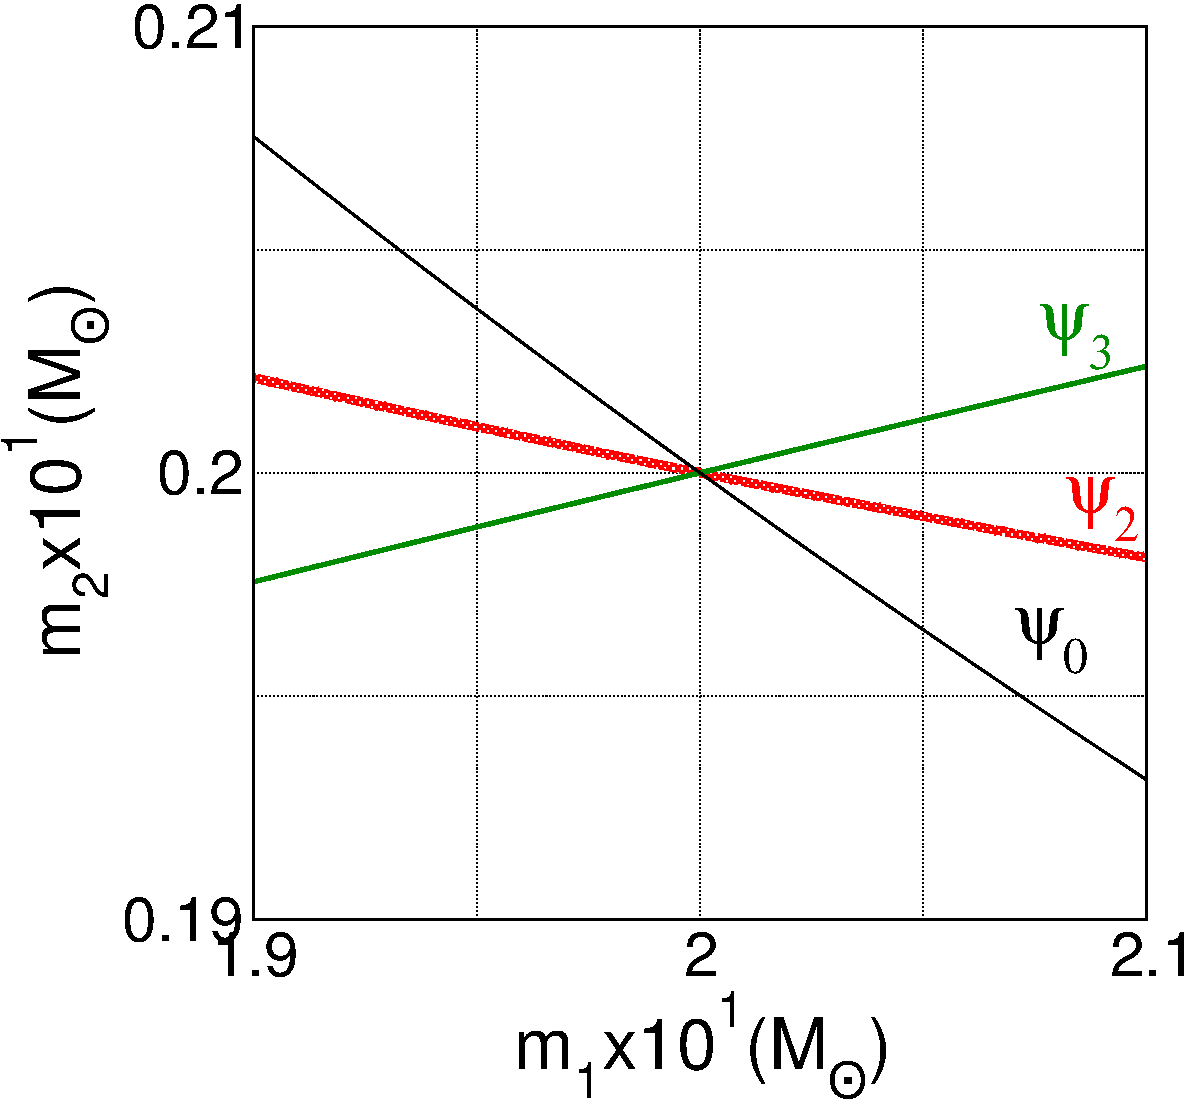
\includegraphics[width=0.34\textwidth]{./Sec_ET_ScienceCase/m1m2_psi3_2e0-2e1.pdf}
%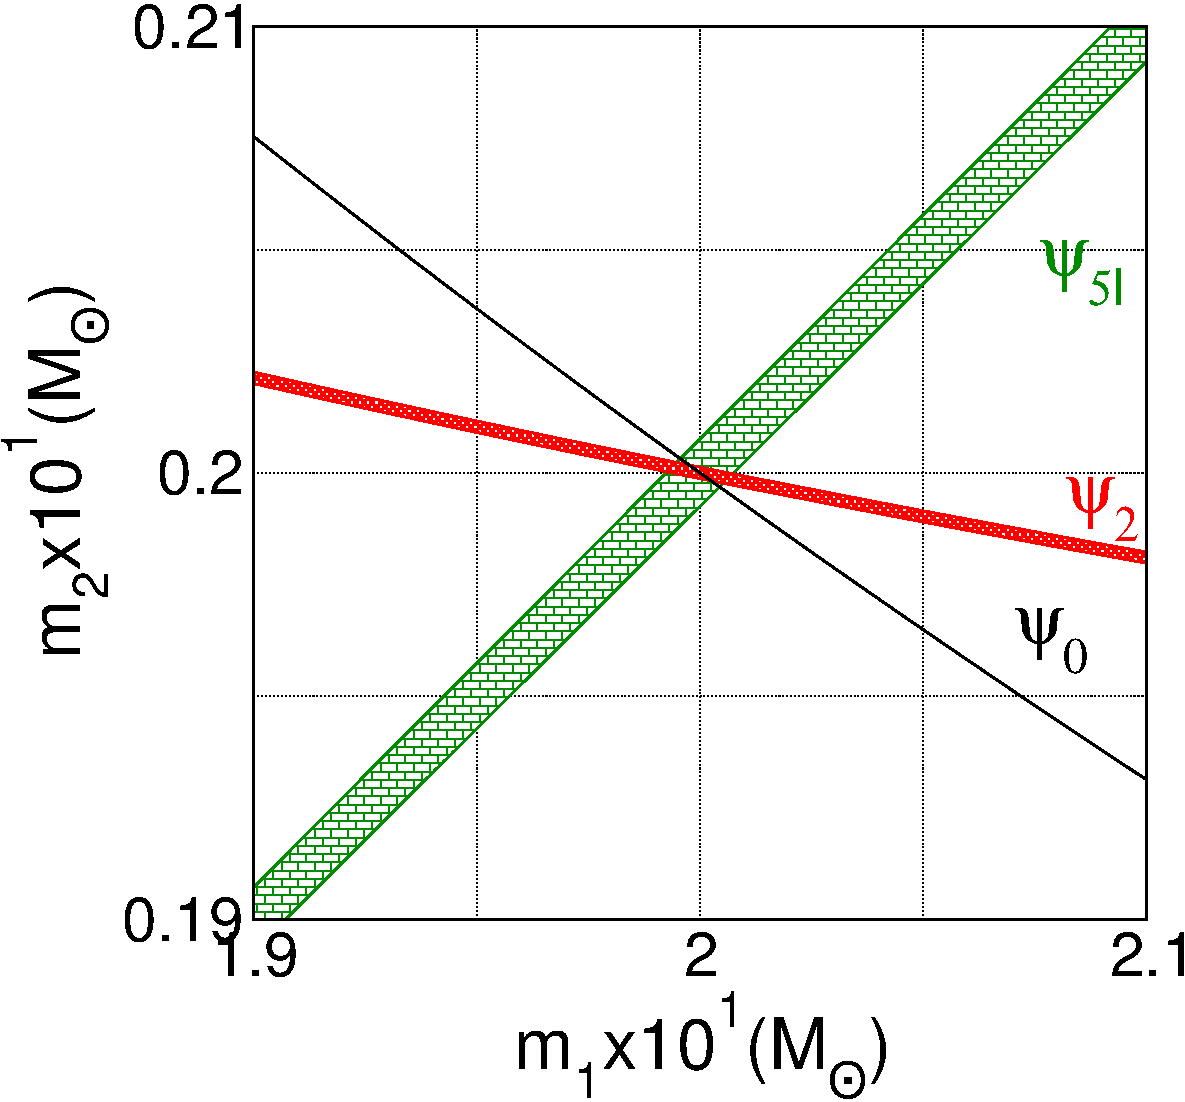
\includegraphics[width=0.45\textwidth]{./Sec_ET_ScienceCase/m1m2_psi5l_2e0-2e1.pdf}
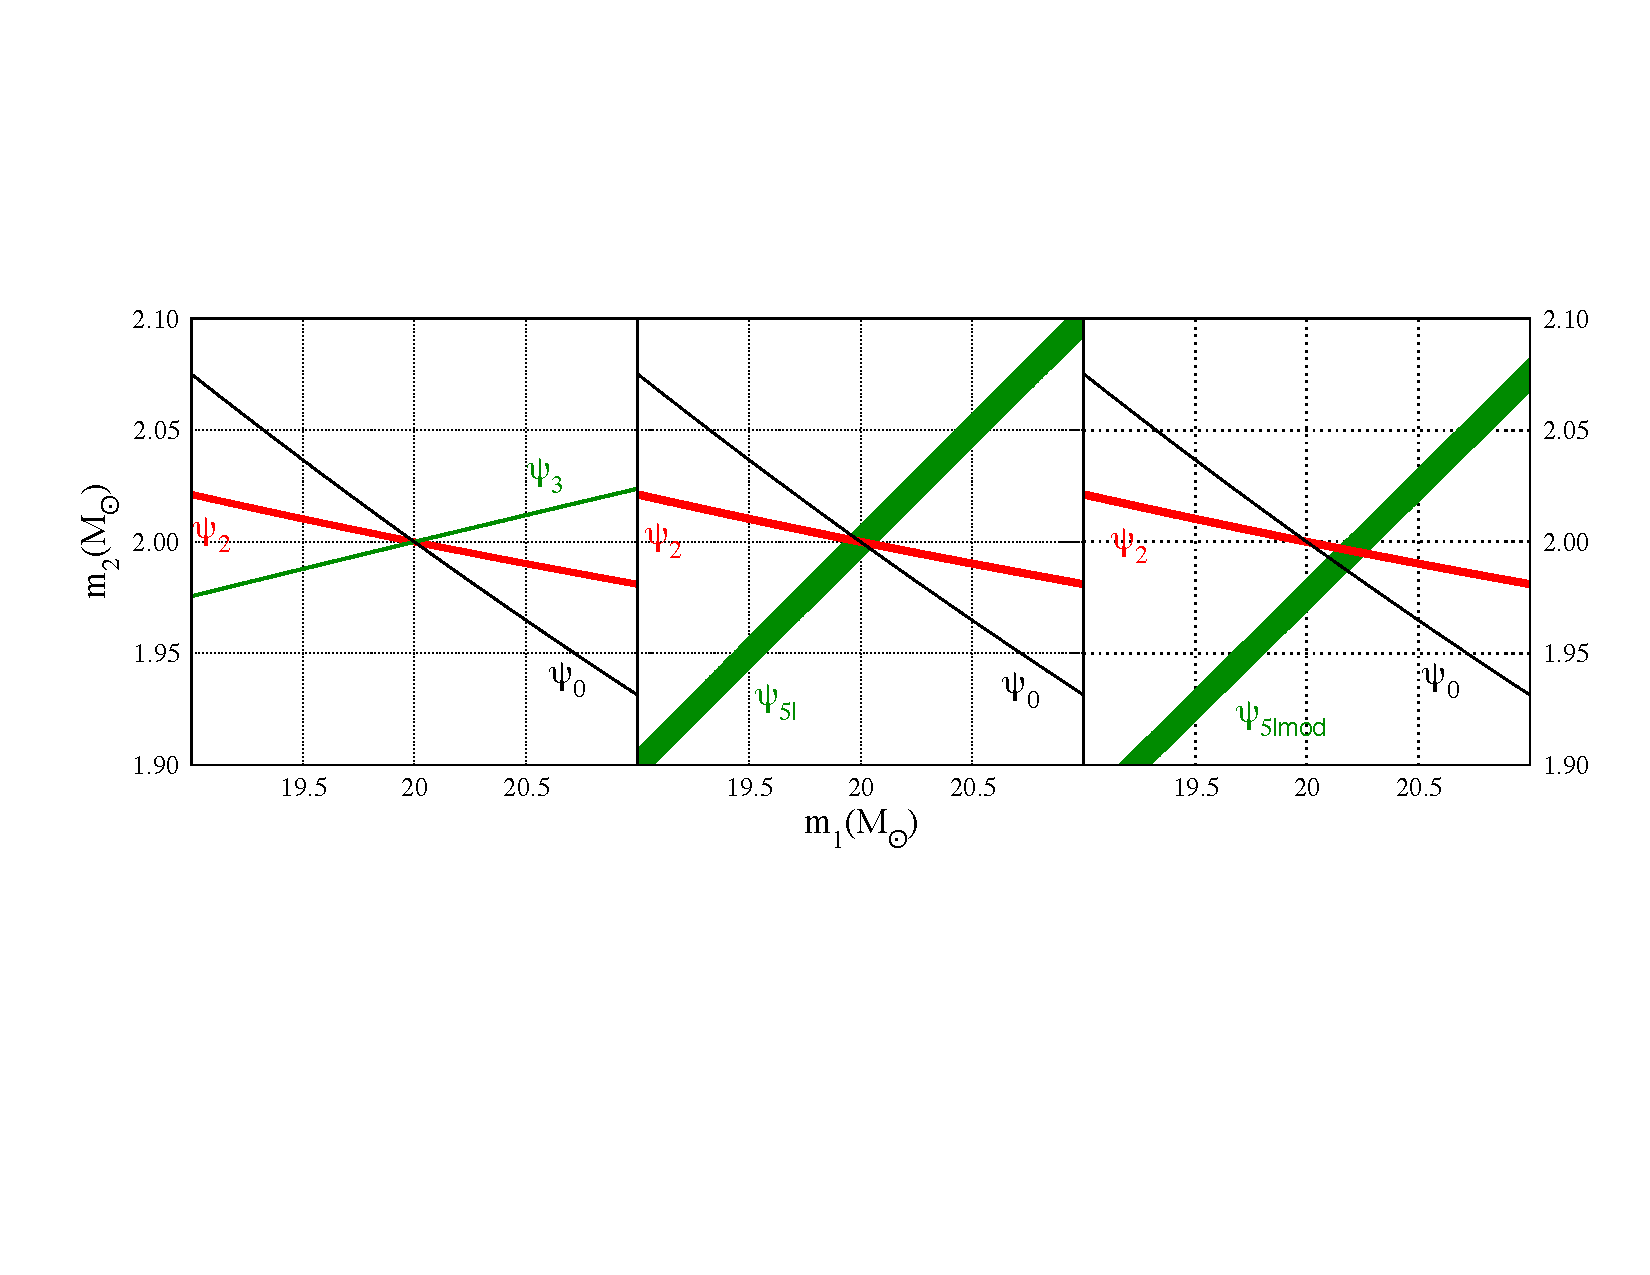
\includegraphics[width=0.95\textwidth]{./Sec_ET_ScienceCase/m1m2_2e02e1_p5lvsp5lmod1p.pdf}

\caption{Curves of constant PN coefficients in the $(m_1,m_2)$ plane 
for a  $(2,20)\,M_\odot$ BBH merger at 300\,Mpc observed in ET-B.  The left 
and middle plots correspond to the case when the post-Newtonian 
coefficients are all as in GR and all three curves intersect at a 
single point. The plot on the right corresponds to the case when the 
measured value of $\psi_{5l}$ differs from GR by 1\% and in this 
case the three curves fail to intersect at a common point.  The
thickness of the lines is the 1-sigma error in the measurement
of the corresponding parameter. \label{fig:m1m2plots}}
\end{figure*}

It is also possible to test for violations of GR without assuming a 
particular alternative model.  One such test was proposed by 
Arun et al.~\cite{testGR:2006,testGR:2007,testGR:2010} and is
based on the post-Newtonian (PN) expansion of the phase of an inspiral 
signal in the frequency domain:
\begin{equation}
\Psi(f) = \sum_{j=0}^7 \left[\psi_j + 
\psi_{jl}\ln(f)\right]\,f^{(j-5)/3},
\label{freqphase}
\end{equation}
where the PN coefficients $\psi_j$ and $\psi_{jl}$,
$j = 0, \ldots, 7$ can be found in \cite{testGR:2010}.
Under the simplifying assumption that spins are zero, these 
coefficients only depend on the component masses $m_1$, $m_2$ of
the binary. Hence only two of these coefficients
are independent, and a possible test of PN theory 
(and hence of GR) is to check for consistency between any three of 
them. Particular attention has been given to $\psi_3$ and $\psi_{5l}$:
\begin{itemize}
\item $\psi_3$ is the lowest-order coefficient which gets contributions from scattering of gravitational
waves off the spacetime near the binary, the so-called tail terms: hence it encapsulates the non-linear
character of GR.
\item $\psi_{5l}$ is the lowest-order coefficient of a logarithmic term in (\ref{freqphase}). General
relativity is not consistent with a simple Taylor expansion.
\end{itemize}
The basic idea of the test is to measure the PN coefficients by fitting the 
observed signal to a model in which three of the PN coefficients, 
instead of two, are treated as independent parameters. As mentioned 
before, each coefficient depends on the two masses $\psi_j=\psi_j(m_1,\,m_2).$
Thus, a measured value of one of the PN coefficients can be used to
draw a curve in the $(m_1,\,m_2)$ plane by inverting the relation
$\psi_j=\psi_j(m_1,\,m_2),$ where the left hand side is the measured value
and the right-hand side is a function only of $m_1, m_2.$ Intersection of
two of the curves, say those corresponding to the measurement of 
$\psi_0$ and $\psi_2$ ($\psi_1$ is identically zero in GR),
gives the component masses. If GR is the correct theory then the curve 
$\psi_3=\psi_3(m_1,\,m_2)$ (left panel of Fig.\,\ref{fig:m1m2plots}) or
$\psi_{5l}=\psi_{5l}(m_1,\,m_2)$ (middle panel of the figure)
will pass through the intersection of the curves corresponding
to $\psi_0$ and $\psi_2.$ If, however, GR is not the correct theory of 
gravity and, say, the value of $\psi_{5l}$ is different from 
that in GR then the curve $\psi_{5l} = \psi_{5l}(m_1,\,m_2)$ will 
not pass through the intersection of the other two curves as in the 
right panel of Fig.\,\ref{fig:m1m2plots}.

In this way, ET will be able to test the non-linear predictions of GR
and confirm whether GR is the correct theory when the gravitational field
becomes so strong that orbital speeds get close to the speed of light.
No other experiments or observations conceived so far can test GR to
such a high order in PN theory.
%The sensitivity at low frequency can have a dramatic effect on the ability to test GR, as shown in Fig.~\ref{fig:lowfreq_testGR}.

%\begin{figure}[h!]
%\centering
%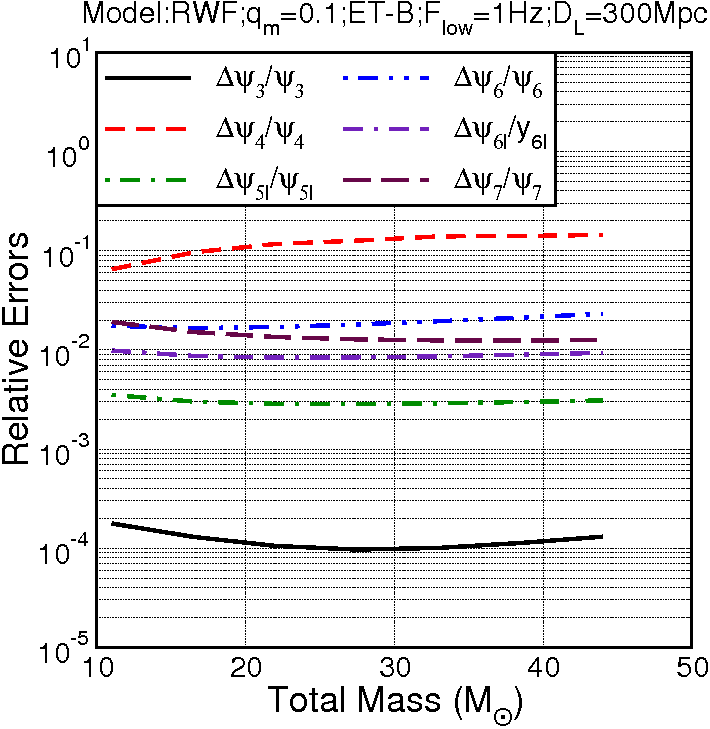
\includegraphics[width=0.45\textwidth]{./Sec_ET_ScienceCase/Errvsmass_RWF_1Hz_0p1_300Mpc.png}
%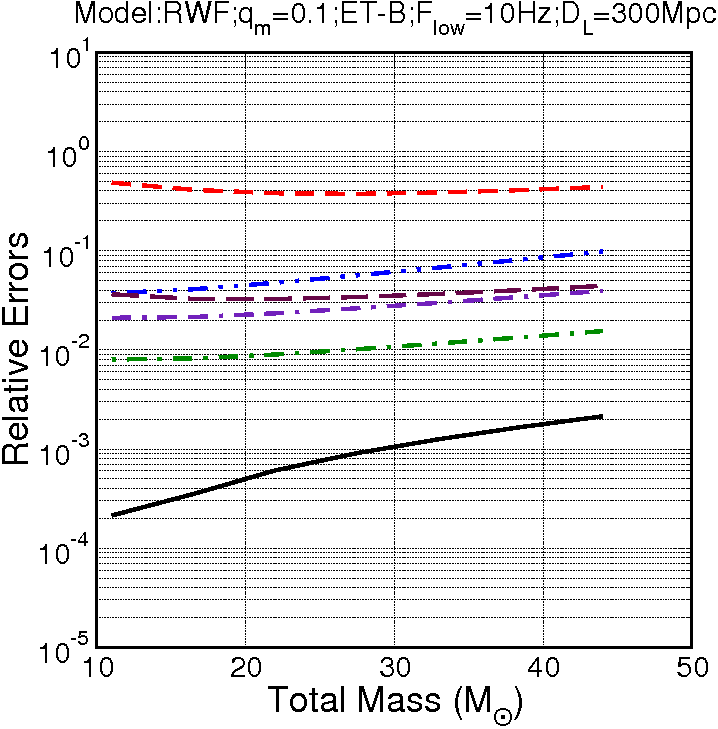
\includegraphics[width=0.45\textwidth]{./Sec_ET_ScienceCase/Errvsmass_RWF_10Hz_0p1_300Mpc.png}
%\caption{Varying the lower frequency cut-off can affect the accuracy in measuring phase coefficients by factors of several
%to an order of magnitude. On the left are relative errors with a 1 Hz cut-off, on the right with a 10 Hz cut-off.}
%\label{fig:lowfreq_testGR}
%\end{figure}


%% \subsection{Test of gravity - 1}
%% \ledby{Bala}

%% \subsection{Test of gravity - 2}
%% \ledby{Bala}
\subsubsection{Measuring the dark energy equation of state
and its variation with $z$}
% \ledby{Van Den Broeck}

Over the past decade, evidence has emerged suggesting that the expansion of the Universe is accelerating. Possible explanations include a failure of general relativity at large length scales, a cosmological constant in the Einstein equations, or a new contributor to the mass/energy content of the Universe called dark energy (DE) (see \cite{PeeblesRatra03} for a review). Assuming a homogeneous and isotropic Universe, DE can be characterized by an EoS of the form $p_{\rm DE} = w(z) \rho_{\rm DE}$, where $p_{\rm DE} < 0$ and $\rho_{\rm DE} > 0$ are the pressure and density, respectively. If the EoS parameter $w(z)$ is constant and equal to $-1$ then this corresponds to having a positive cosmological constant in the gravitational field equations. Current constraints allow for this possibility, but other possibilities are not ruled out. The seven year WMAP data combined with Type Ia supernova measurements and baryon acoustic oscillations in the galaxy distribution lead to the constraint $w = -1.10 \pm 0.14$ at the 68\% confidence level \cite{WMAP7}.

The GW signal from inspiraling compact binaries is particularly ``clean" and well-understood. Consequently, as suggested by Schutz, one can think of using inspiral events as ``standard sirens", much in the way Type Ia supernovae have been used as standard candles \cite{Schutz86}. From the GW signal itself the luminosity distance $D_{\rm L}$ can be inferred, but not the redshift. However, if a particular compact binary coalescence event is accompanied by a sufficiently distinct electromagnetic counterpart, then it will be possible to find its position in the sky, identify the host galaxy, and obtain the redshift $z$. The relationship $D_{\rm L}(z)$ depends sensitively on cosmological parameters such as the Hubble constant at the current epoch $H_0$, the normalized matter and DE densities $\Omega_{\rm M}$ and $\Omega_{\rm DE}$, and the DE EoS parameter $w$. For example, in a spatially flat FLRW Universe and assuming a constant $w$,
\begin{equation}
D_{\rm L}(H_0, \Omega_{\rm M}, \Omega_{\rm DE}, w; z) = (1+z)\,\int_0^z \frac{dz'}{H_0 \left[ \Omega_{\rm M}(1+z')^3 + \Omega_{\rm DE} (1+z')^{3(1+w)} \right]^{1/2}}.
\label{DLgeneral}
\end{equation}
The intrinsic luminosity, and hence the luminosity distance, of an inspiral GW event can be inferred directly from the amplitude of the observed waves and from the component masses, which govern the structure of the signal. Thus, unlike Type Ia supernovae, their calibration does not depend on the brightness of other sources. Thus GW astronomy opens up the possibility of cosmography \emph{without having to rely on the lower rungs of the cosmic distance ladder}.

Compact binary coalescences that involve a NS are assumed to have strong electromagnetic counterparts, mostly in the form of strongly beamed gamma radiation directed perpendicularly to the plane of the inspiral. Such events are believed to be the progenitors of short, hard Gamma Ray Bursts (GRBs): if the beam roughly points towards Earth then a flash of gamma radiation is seen, followed by an afterglow in the lower-frequency electromagnetic spectrum.
This would then allow us to identify the host galaxy and obtain a redshift.

The GW signal from a NSBH coalescence will be visible out to $z = 3.5$. Within the corresponding volume, it is reasonable to expect $\sim 10^4$ or more such coalescences per year, but depending on the opening angle of the gamma ray beam only a few percent of these will be visible as a GRB. Hence we should have a few hundred sources at our disposal for which the redshift can be measured. The uncertainty on $z$ will be negligibly small, while $D_{\rm L}$ will be measurable with $\sim 3$\% inaccuracy at $z = 1$, rising to $\sim 10$\% at $z = 3.5$. Fitting the measured values of $D_{\rm L}$ against redshift by varying $H_0$, $\Omega_{\rm M}$, $\Omega_{\rm DE}$, and $w$ in the relationship (\ref{DLgeneral}) should then allow for the determination of these cosmological parameters with uncertainties of 5\% or better, as discussed further in Section~\ref{cosmo_parameters}.

\subsubsection{Testing the uniqueness theorem of black hole spacetimes}
\label{subsubsec:uniquenesstheorem}
It is generally accepted that the compact objects observed in 
the centres of most galaxies are massive, rotating BHs described by 
the Kerr metric of GR. This belief comes in part from the uniqueness 
theorem, which states that the Kerr metric is the unique end state 
of gravitational collapse~\cite{carter71}. However, this theorem is 
based on several assumptions -- the spacetime is vacuum, axisymmetric 
and stationary; there is a horizon in the spacetime; and there are no 
closed timelike curves. If one of these assumptions were violated, 
then objects that deviate from the Kerr metric could exist.
\begin{figure}
\centering
\begin{tabular}{|c|c|}
\hline
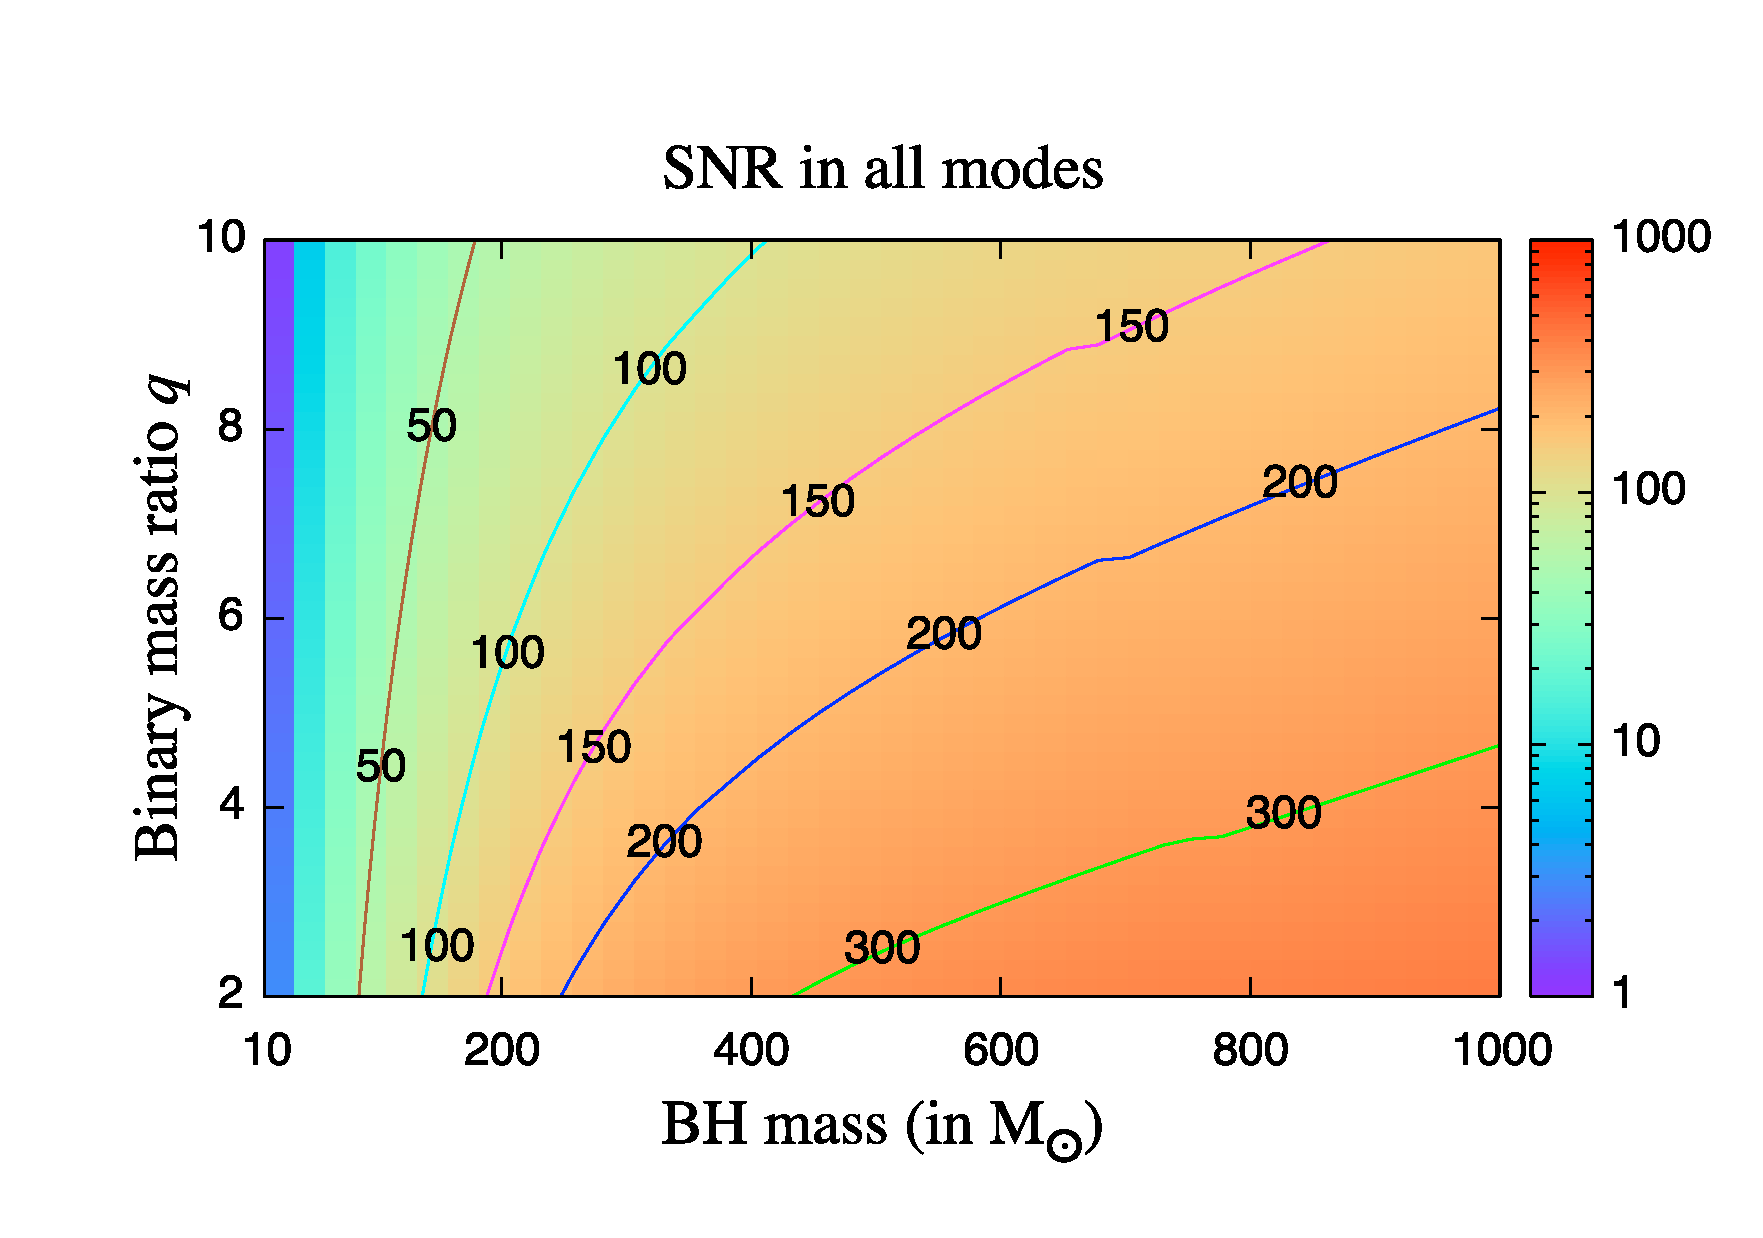
\includegraphics[width=0.45\textwidth]{./Sec_ET_ScienceCase/ET-SNR-all.pdf}  &
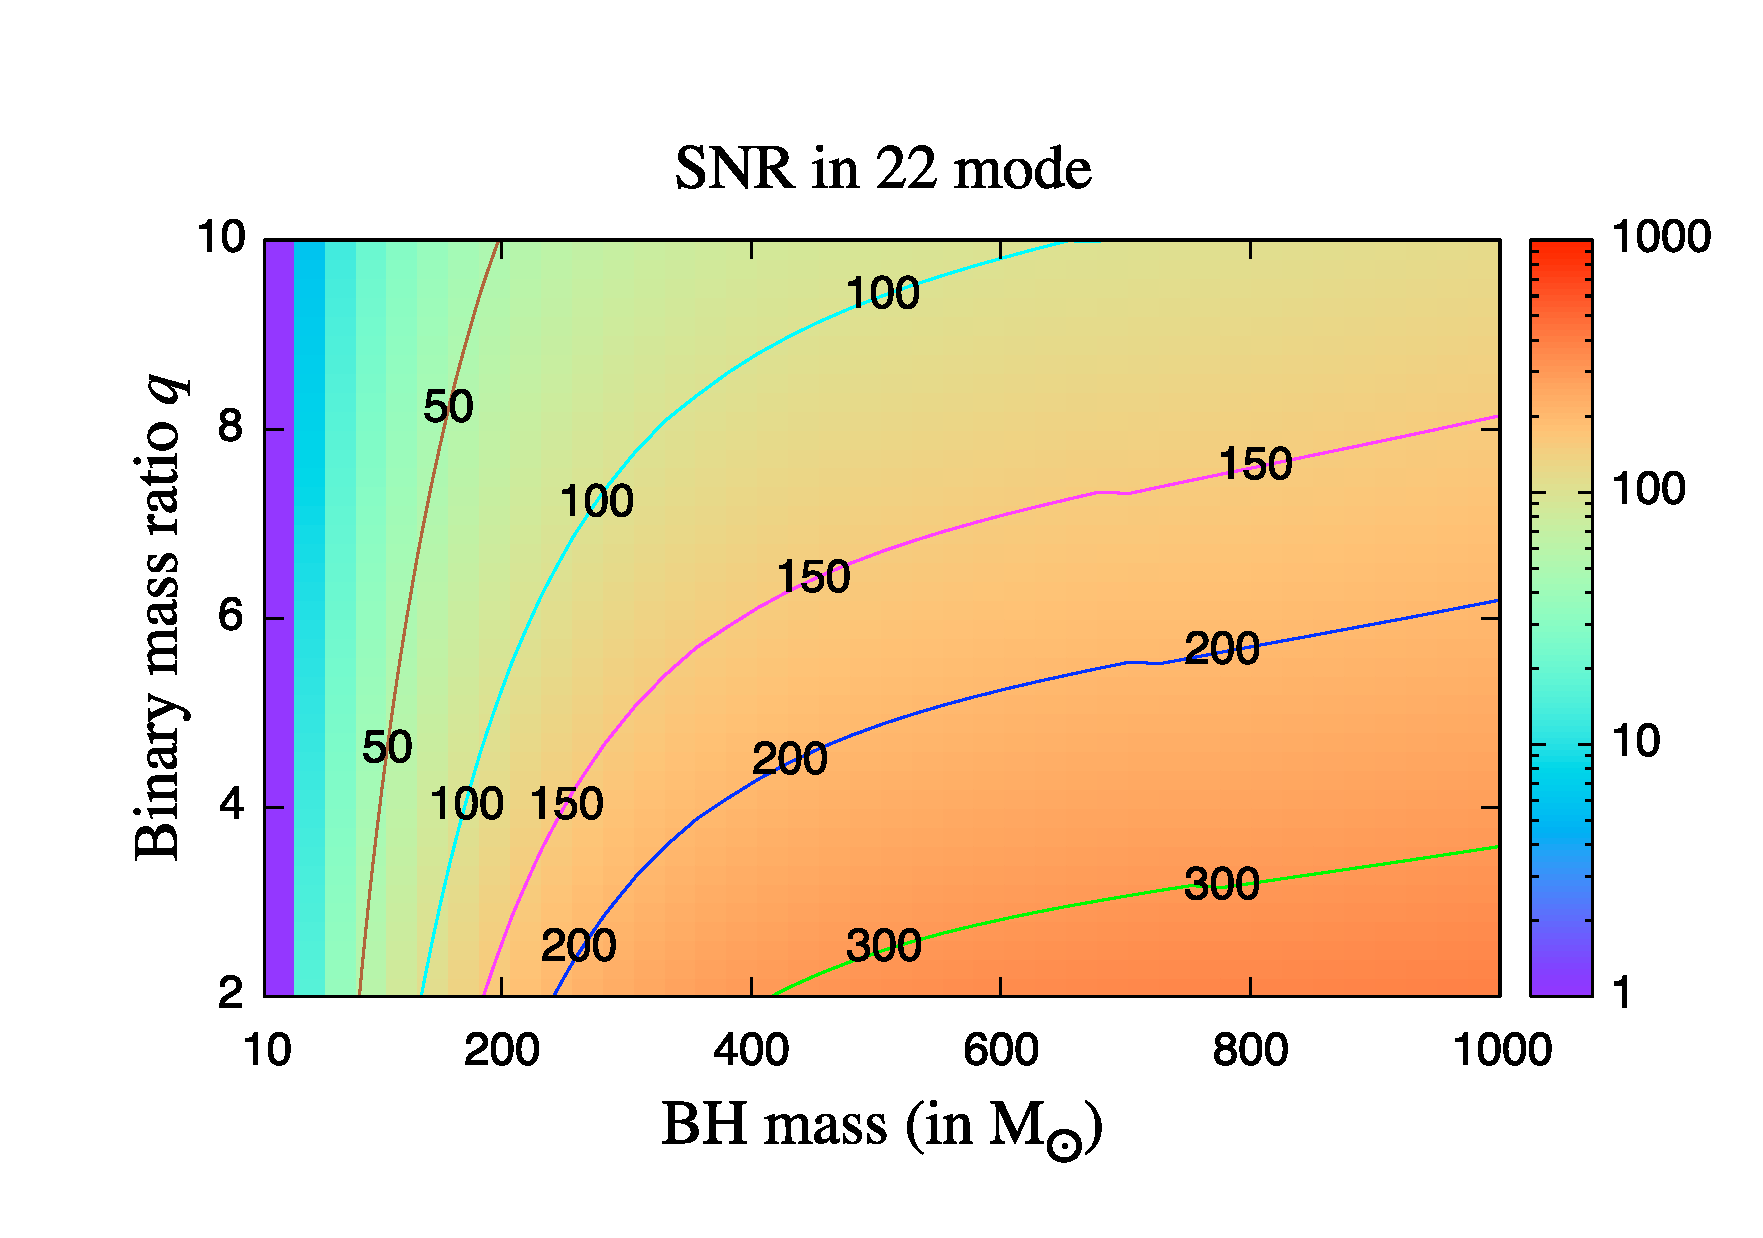
\includegraphics[width=0.45\textwidth]{./Sec_ET_ScienceCase/ET-SNR-22.pdf} \\
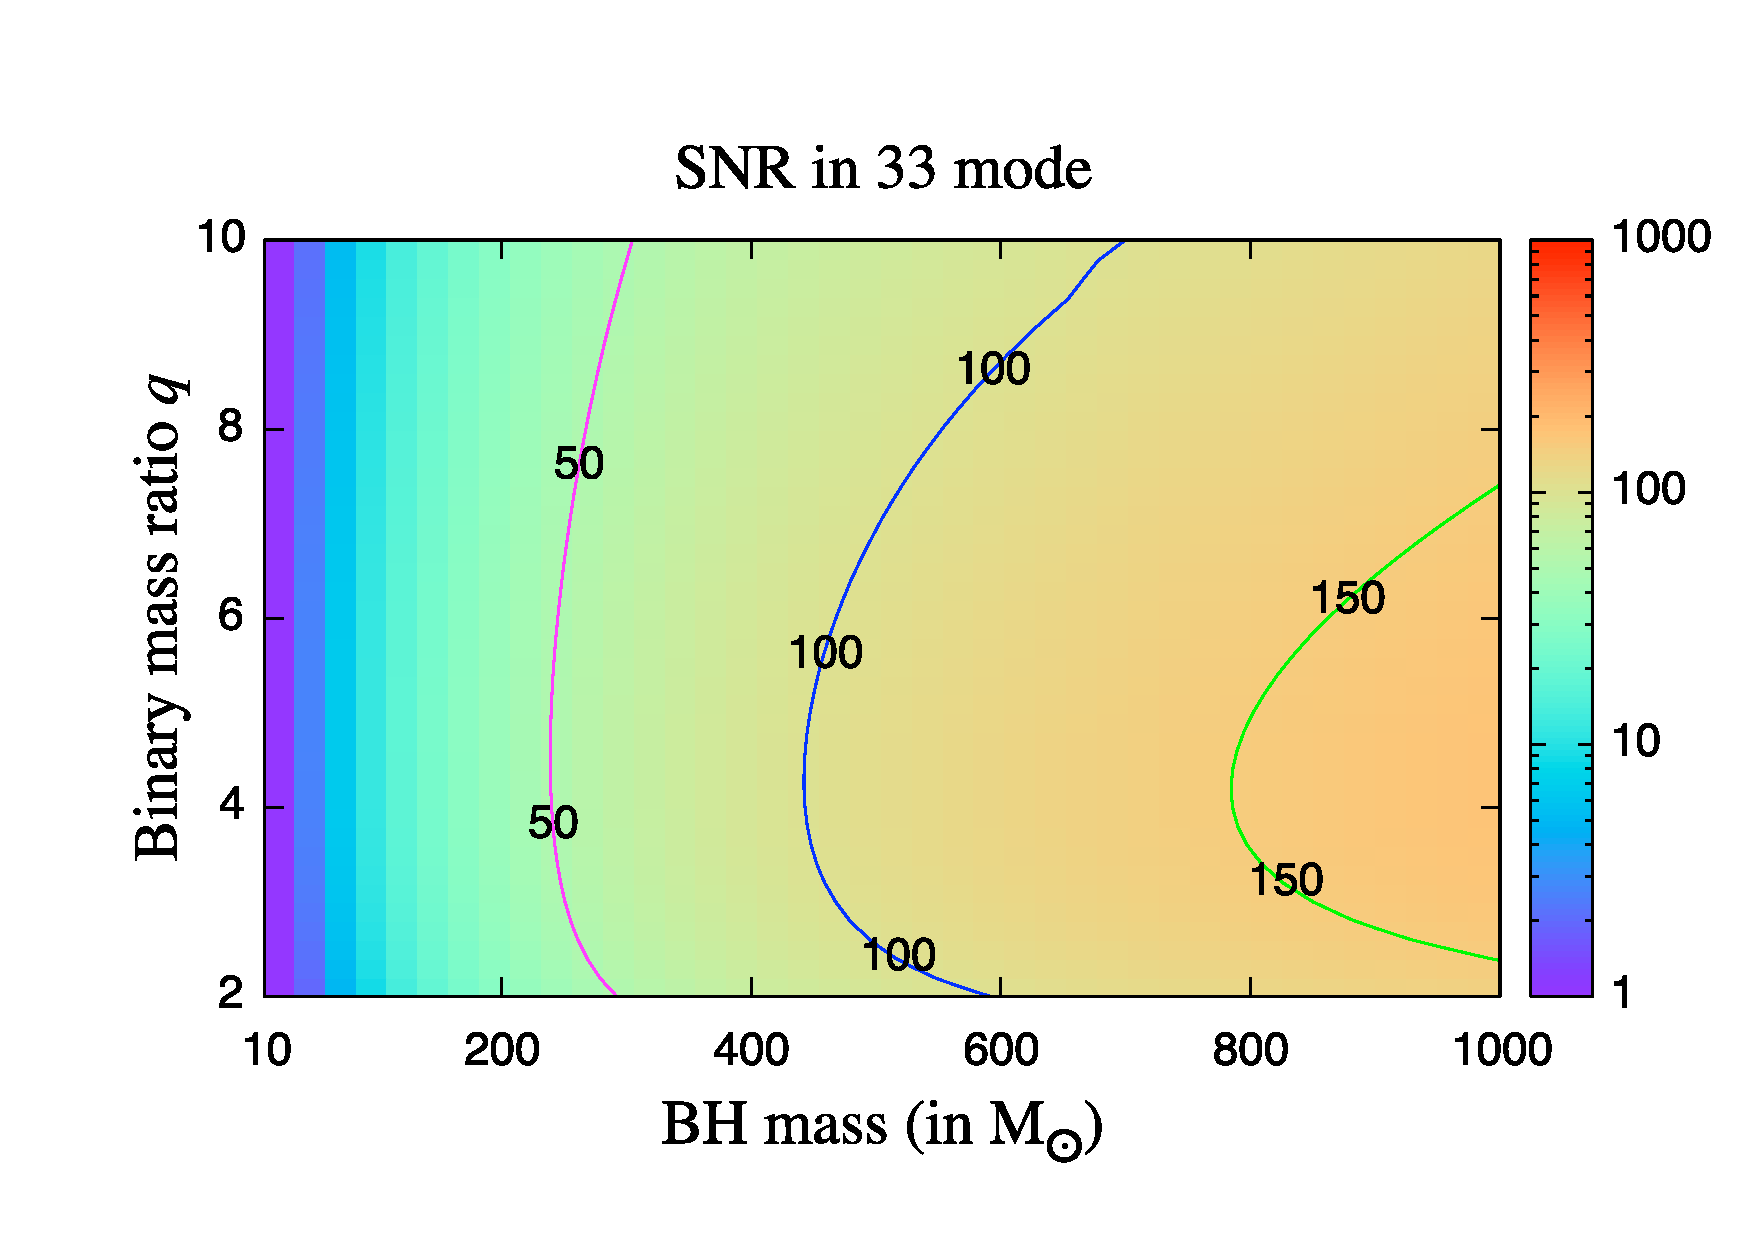
\includegraphics[width=0.45\textwidth]{./Sec_ET_ScienceCase/ET-SNR-33.pdf} &
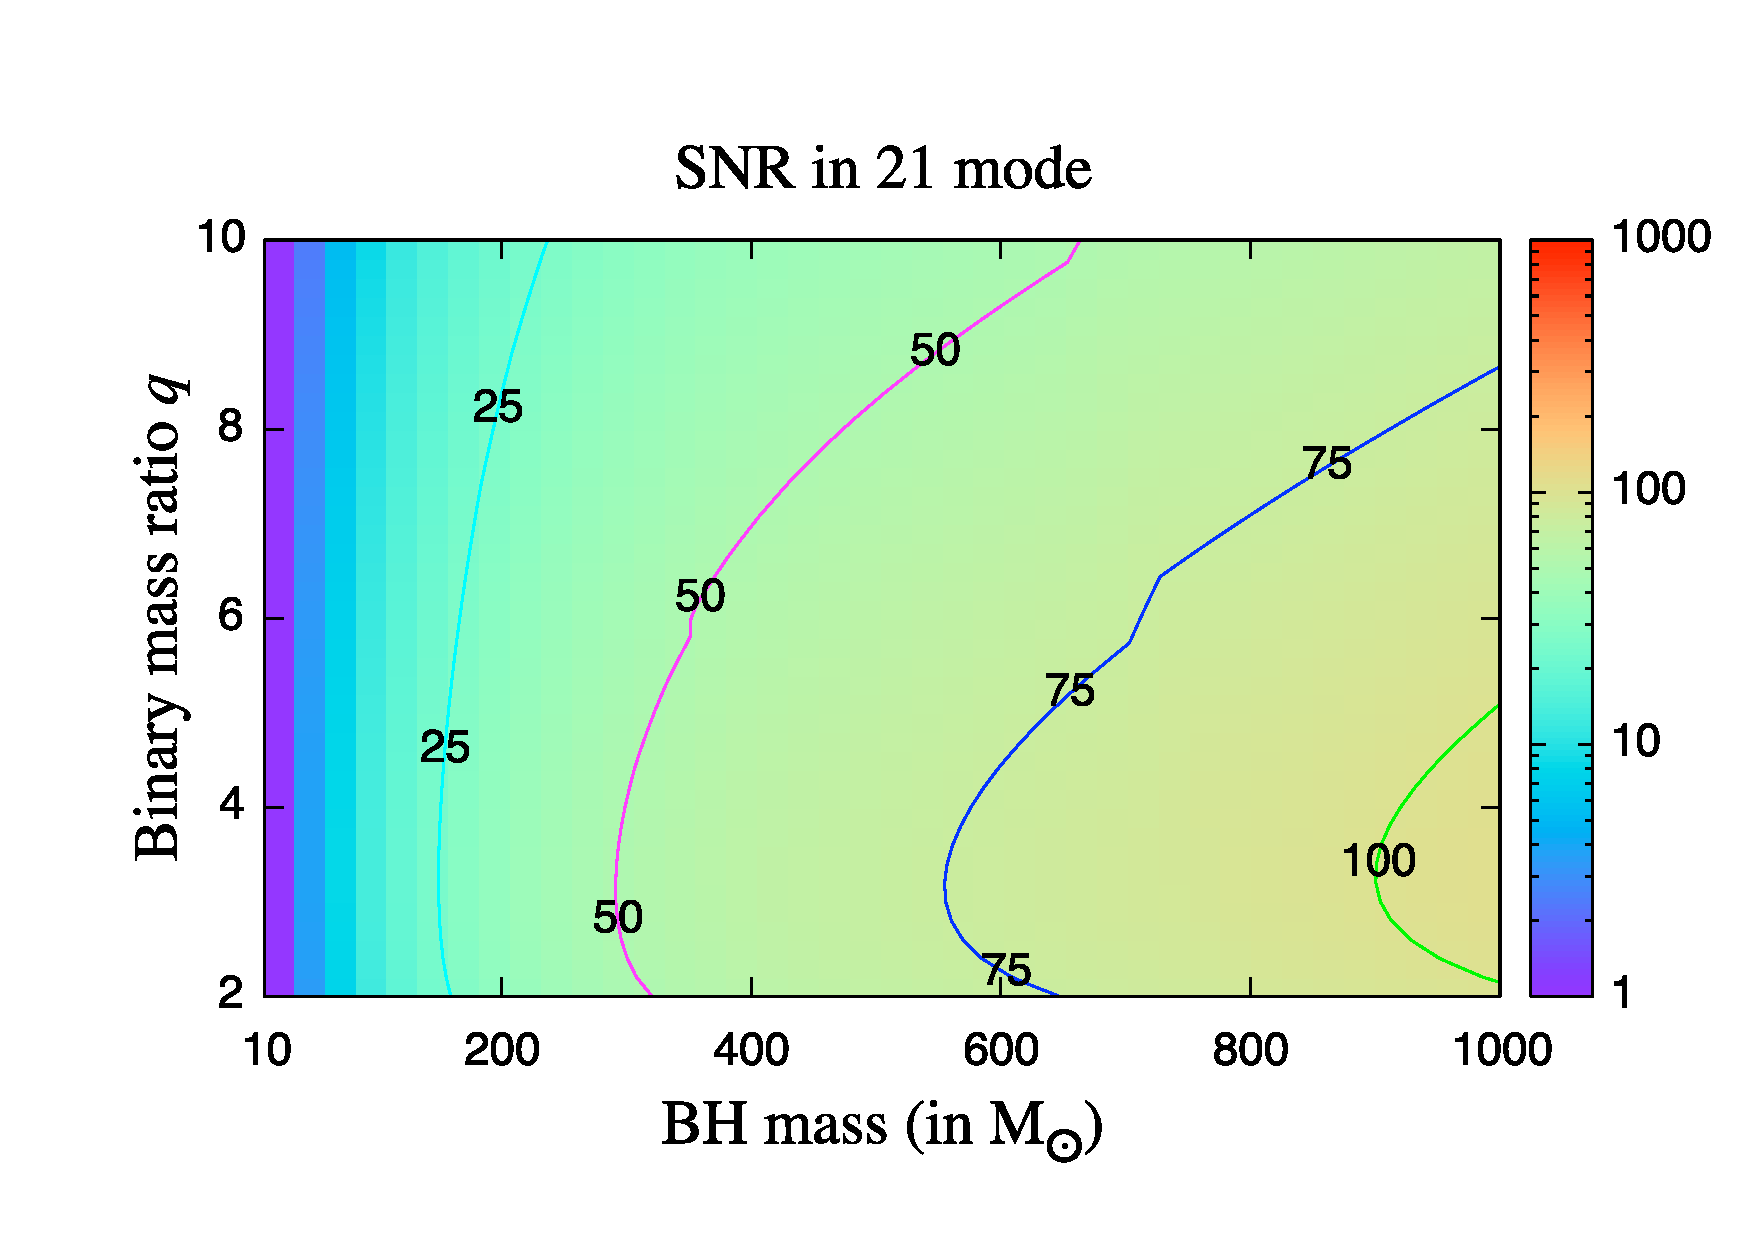
\includegraphics[width=0.45\textwidth]{./Sec_ET_ScienceCase/ET-SNR-21.pdf} \\
\hline
\end{tabular}
\caption{Signal-to-noise ratio of quasi-normal modes in ET as a 
function of the BH's mass $M$ and progenitor binary's 
mass ratio $q$ for different modes. Most of the contribution to the 
SNR comes from the 22 mode but other modes too have significant 
contributions, 33 being more important than 21.} 
\label{fig:snr}
\end{figure}

In BBH systems where one component is much heavier than the other, 
many GW cycles are emitted while the smaller object is in the strong 
field region close to the larger object. These GWs encode a map of 
the spacetime structure in the vicinity of the large BH, which can be 
used to measure properties of the central object~\cite{ryan95}. Using 
such observations to measure spacetime structure has been explored 
extensively in the context of extreme-mass-ratio inspirals (binaries 
of $\sim10M_{\odot}$ objects with $\sim 10^6M_{\odot}$ objects) 
for LISA (see~\cite{AmaroSeoane:2007aw} and references therein). 
There is an analogous source for ground based detectors, namely the 
inspiral of a $\sim1M_{\odot}$ object into a $\sim100M_{\odot}$ BH. 
We refer to these as intermediate-mass-ratio inspirals (IMRIs)~\cite{LIGOimri}.


ET will be able to detect IMRIs out to redshifts $\sim 1$--$5$, 
depending on the mass and spin of the central IMBH \cite{Huerta:2011}. 
Assuming that $\sim10\%$ of globular clusters form IMBHs, ET will detect 
between a few tens and a few hundreds of events, depending on the 
mass distribution of the intermediate mass BHs \cite{Gair:2009ETrev}. The 
biggest uncertainty is in the intrinsic density of IMBHs, which could 
reduce these numbers by several ordrs of magnitude. Advanced LIGO 
observations of IMRIs could be used to make very modest measuements 
of deviations in BH structure from the Kerr metric, e.g., 
an ${\cal O}(1)$ deviation in the quadrupole moment~\cite{LIGOimri,imrirate}. 
ET will observe IMRI events for many more cycles, due to its better 
low-frequency performance, which is very important for the precision of 
spacetime mapping measurements. We would therefore expect to obtain 
constraints that are one or two orders of magnitude better with ET, 
although explicit estimates of this have not yet been made.

\subsubsection{Testing the no-hair theorem using BH quasi-normal modes}
Perturbed Kerr BHs emit gravitational radiation 
which consists of a superposition of damped sinusoids termed 
quasi-normal modes.  The frequencies and time-constants of the modes 
depend only on the mass and spin of the BH --- a consequence 
of the no-hair theorem. It has been proposed that a measurement 
of two or more quasi-normal modes could be used to confirm that the 
source is a BH and to test if GR continues to hold
in ultra-strong gravitational fields.

The fundamental mode frequencies and time constants, characterized 
by two indices $(\ell,m)$, $\ell=2,3,\ldots$ and $m=-\ell,\ldots,\ell,$
are given by the general expressions
\begin{equation}
\omega_{\ell m} = \frac{F_{\ell m}(j)}{M},\quad
\tau_{\ell m} = M G_{\ell m}(j),
\end{equation}
where $F_{\ell m}(j)$ and $G_{\ell m}(j)$ are functions of 
the dimensionless BH spin magnitude, or Kerr parameter, $j$.  
Not all modes are excited equally; when, for instance, two BHs
merge to form a single BH the $(\ell,m)=(2,2)$ mode is the
most dominant followed by $(\ell,m)=(3,3)$ and so on. However,
all mode frequencies and time-constants depend only on the mass 
$M$ and (dimensionless) spin magnitude $j=J/M^2,$ where $J$ is
the magnitude of the BH's spin angular momentum. 
Several authors have noted that this 
aspect of the no-hair theorem could be used to test if massive 
compact objects at galactic cores are actually rotating BHs 
described by the Kerr metric of general relativity 
\cite{BHspect04,BCW05,Berti:2007a}; alternatively, it could be used 
as a strong field test of GR itself \cite{BHspect04}. 

The key idea behind the proposed tests is the following: If one can reliably 
decompose the observed gravitational radiation from a ringing BH into 
a superposition of different modes, then the frequencies and time-constants of 
each of the modes could be used to infer the mass and spin of the BH.
If the object is truly a BH, then the masses and spins obtained
from the different modes should all be consistent within the measurement
errors. Inconsistencies in the values of the masses and spins inferred 
from different modes would be an indication of the failure of GR or that the
radiation was emitted from an object that is not a BH. If a merging
binary does not lead to a BH then the inspiral phase may not
result in a superposition of QNMs that can be characterized by 
just two parameters.  

Figure \ref{fig:snr} plots the SNR in the ringdown
signal (plot titled ``SNR in all modes") and contribution from 
the $(\ell,m)=(2,2), (2,1)$ and (3,3) modes 
as a function of the mass $M$ and mass ratio $q=m_1/m_2$ ($m_1>m_2)$
of the progenitor binary.  Although the (2,2) mode is the most dominant, 
the other modes are large enough that it should be possible to 
disentangle the different modes and test the no-hair theorem.

\paragraph{Testing the no-hair theorem by measuring the multipole 
moments of a source}
There is an alternative way to test the no-hair theorem.
Another consequence of this theorem is 
that the entire spacetime structure, characterised by 
``multipole moments'', is determined by just two parameters, the BH 
mass, $M$, and spin parameter, $S=J/M,$ where $J$ is the magnitude of
the spin angular momentum. It has been demonstrated 
that GW observations can measure the mass and spin multipole moments 
$M_l$ and $S_l$ independently of one another~\cite{ryan95}. We can, 
therefore, directly verify that they satisfy the Kerr relationship
$ M_l + i\,S_l = M(i\,S/M)^l\,. $
We would only need to measure three multipole moments to rule out 
an object as a Kerr BH.

It has been shown that IMRI observations with Advanced LIGO could 
detect an $\mathcal{O}(1)$ deviation in the quadrupole moment of 
an object~\cite{LIGOimri}. The precision achievable with ET should 
be at least a factor of $10$ better than this due to the improved 
low-frequency performance. To put this in perspective, one alternative 
to BHs, boson stars, have quadrupole moments two orders-of-magnitude 
bigger than BHs of the same mass and spin~\cite{ryanBS}.

Any deviations from the no-hair theorem that are detected will have 
profound implications for our understanding of relativity and of BHs. 
Persistent deviations from the theory may lead to important insights 
in the search for a fundamental theory that unifies all four forces 
of nature.
\paragraph{Are there naked singularities?}
% \ledby{Gair}
One of the assumptions of the uniqueness theorem is that a horizon exists in the spacetime. This arises from a belief embodied by the ``Cosmic Censorship Hypothesis''~\cite{CCH} (CCH), which states that any singularity will be enclosed by a horizon. The CCH arises from a desire for predictability in the Universe---when Physics breaks down at a singularity, we do not want information from that to propagate into the rest of the Universe. However, the CCH is unproven and therefore ``naked'' singularities not enclosed within a horizon may still exist. Gravitational wave observations provide a unique way to look for these exotic objects. Observations may be indirect, via detection of a violation to the ``no-hair'' theorem. However, they may also be direct---if a horizon is not present in the spacetime, the gravitational waves will not cut off when the object crosses the horizon~\cite{kesden05}, which will be a clear smoking gun signature for the absence of a clothing horizon in the system.

ET will provide much more stringent constraints on potential violations of the CCH than are possible with Advanced LIGO. ET observations will therefore play an important role in answering the question as to whether naked singularities exist, which could have profound implications for our understanding of various aspects of the theory of relativity.

%\subsubsection{Measuring the mass of neutrinos via supernovae}
%CVDB\\
%\dots

\subsubsection{Limit on the maximum mass of compact stars}

It is generally believed that NSs have masses
between $\sim 1.3\,M_\odot$ and $\sim 2\,M_\odot,$ % [CITATION],
but such statements rely on guesses regarding the EoS of
dense nuclear matter. Above $2\,M_\odot$ a quark star might be created, or
some other exotic object.  Apart from the existence of such objects 
and their properties, an interesting question is how massive
a star can be while still being stable. 

\begin{wrapfigure}{l}{0.5\textwidth}
\vskip -0.3cm
%\begin{figure}
\centering
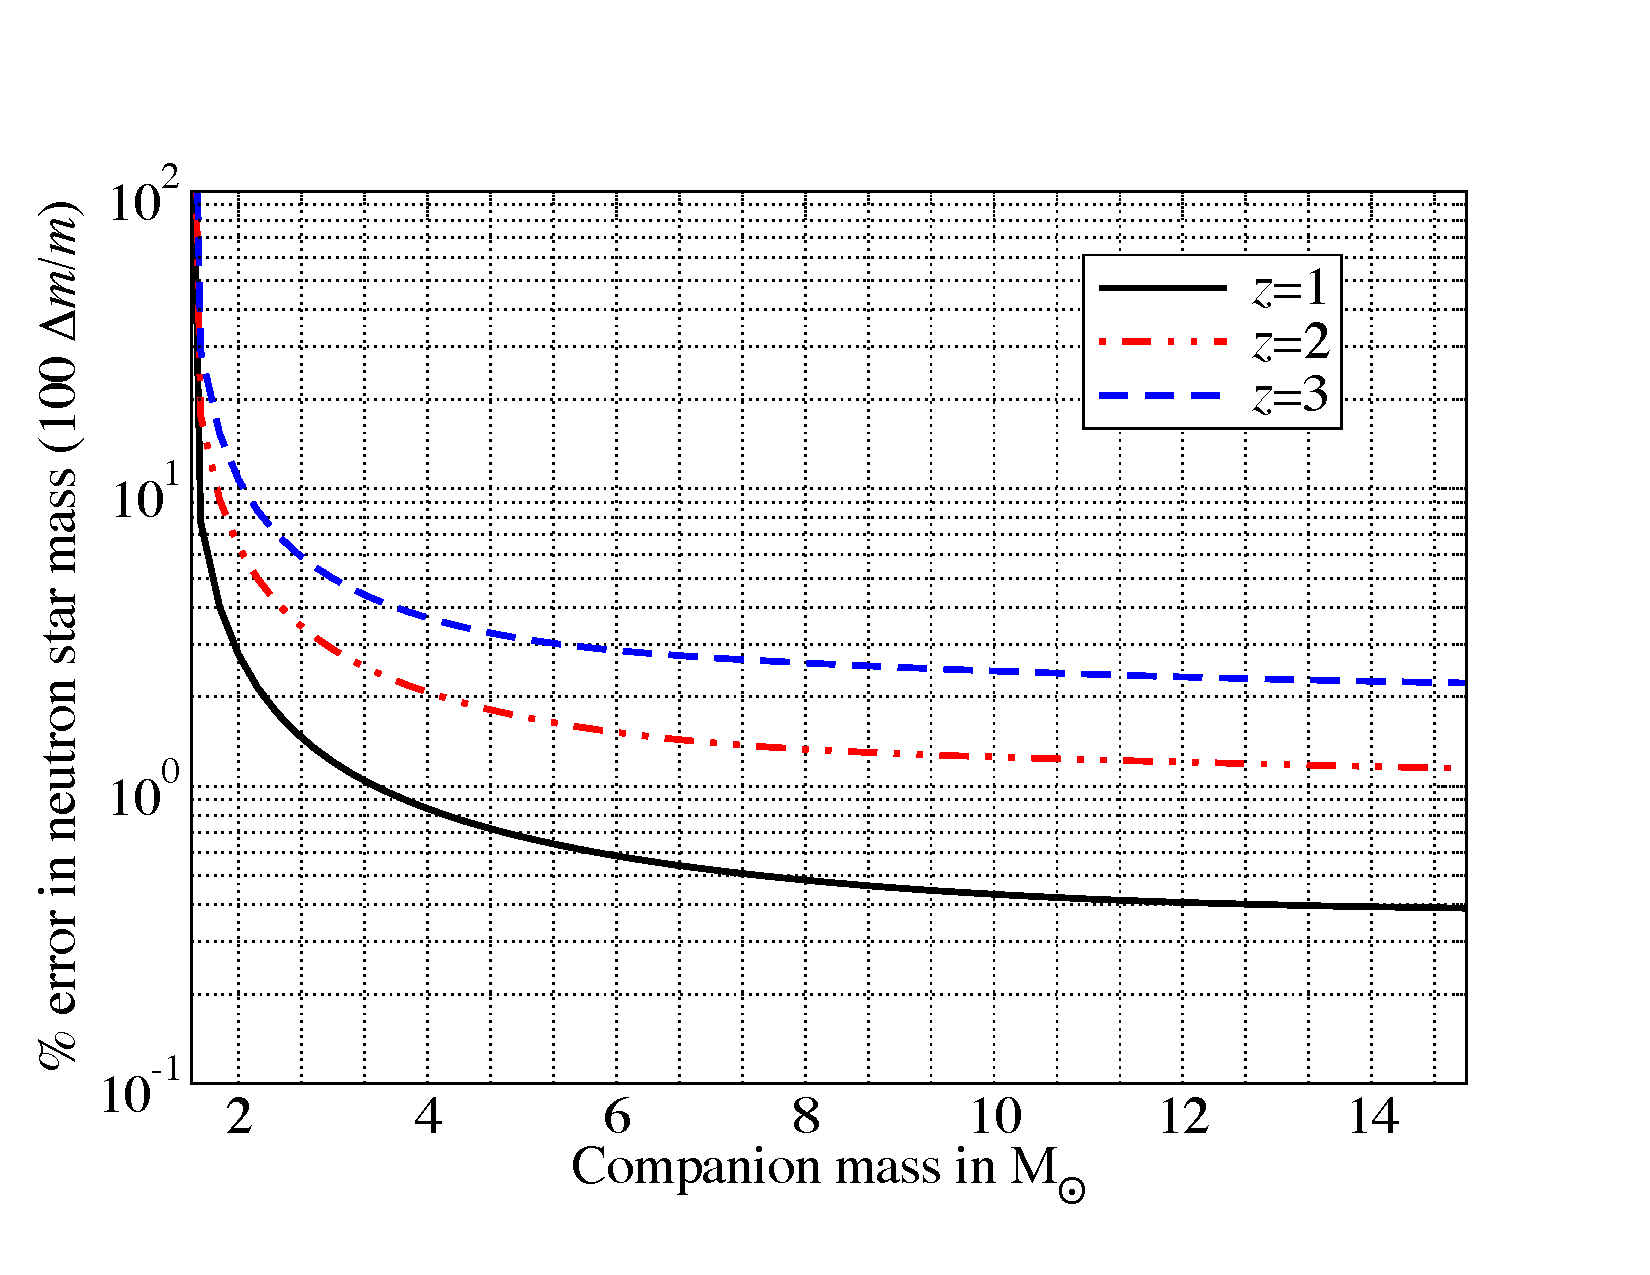
\includegraphics[angle=0,width=0.5\textwidth]{./Sec_ET_ScienceCase/NSmass.pdf}
\caption{The accuracy with which the mass of a neutron star can be 
determined, as a function of the mass of the companion object.}
\label{fig:NS_MassAccuracy}
%\end{figure}
%\vskip 0.9cm
\end{wrapfigure}
Fig.~\ref{fig:ET_range} shows the maximum distance
to which binary inspirals can be seen in ET for systems
with two equal mass companions. The distance reach for a binary
with symmetric mass ratio $\nu$ would be smaller by a 
factor\footnote{A factor of $\sqrt{4\,\nu}$ can be understood in
the following manner: The signal-to-noise ratio of an inspiral
signal is directly proportional to the product of its amplitude 
(which goes as $\nu$) and square-root of its duration (which
goes as $\nu^{-1}$), or an overall factor of $\sqrt{\nu}.$ A
factor of 4 is included for normalization as $\nu=1/4$ for equal
mass systems.} of $\sqrt{4\,\nu}$. For a NS of $2\,M_\odot$ and a
BH of $5\,M_\odot,$ $\nu\sim 0.20$ and so the range would be 
90\% of that for a binary composed of two $3.5\,M_\odot$ system.
Considering NS masses of $1.4\,M_\odot$ and BH masses of $10\,M_\odot$
one gets the distance reach to be $56\%$ of that for a binary
of total mass $16.4\,M_\odot$ and composed of two equal mass
BHs.  The above reasoning shows that ET will have access
to NSBH sources out to genuinely cosmological distances, up to
redshifts of several, with an expected detection rate in the
order of $10^6\,\mbox{yr}^{-1}$. 

Fig.~\ref{fig:NS_MassAccuracy}
shows how accurately ET will measure the mass of a NS 
(assumed to be $1.4\,M_\odot$) in an NSBH
inspiral process, as a function of the mass of the BH for three
different values of the redshift, $z=1,2,3.$ We see that for BH masses 
larger than $2\,M_\odot$ the NS mass is measured to better than
$10\%.$ Indeed, most astronomical BH candidates have a 
minimum mass of $\sim 4\,M_\odot$ and for BH mass $\gtrsim 4\,M_\odot$, 
the NS's mass can be inferred to a fraction of a percent out to
$z=1$, and up to a few percent out to a redshift of 2 or 3. This
would enable us not only to establish the mass distribution of
NSs and possible dense exotic objects, but also the 
evolution of this distribution over cosmological timescales.

\clearpage
\FloatBarrier

\subsection{Astrophysics}
ET will be a unique observatory in many ways to study neutron stars 
and black holes.  It will be sensitive to relativistic phenomena that 
efficiently convert energy in non-axisymmetric motion in compact
objects into gravitational waves. Examples include quakes in neutron 
stars, supernovae, proto-neutron stars, inspiralling and colliding 
binary neutron star and neutron star-black hole systems and gamma-ray 
burst sources, systems and phenomena where motion ought to be 
highly relativistic and hence potential sources of GW too.
In this Section we will look at what ET can unveil about compact 
objects and their environs.

\subsubsection{Determining the neutron star equation of state from 
binary coalescences}

% \ledby{Rezzolla, Read}
% \textcolor{blue}{Probing the ground-state of nuclear state over a
% range of nuclear density, measuring the effects of neutron star
% equation of state using binary neutron star mergers, and measuring
% magnetic fields, post-merger oscillations}

Several BNS systems have been observed to date, for some of which
general-relativistic effects in the binary orbit have been measured 
to high precision \cite{Living:Lorimer}. The inspiral and merger of 
two NSs in binary orbit is the inevitable fate of close-binary
evolution, whose main dissipation mechanism is the emission of
GWs.  The detection of GWs from
NS binaries will provide a wide variety of physical
information on the component stars, including their mass, spin, radius
and EoS.  The central densities of isolated
NSs, in fact, can range up to ten times the nuclear saturation
density, and during the merger and coalescence of two NSs
the maximum density will rise even further, before the remnant object
collapses to a BH.  The behaviour of bulk matter at these
densities is not well understood; measurements of GW
signals from NS sources can usefully constrain the
EoS at these densities.

Quantum chromodynamics is expected to be a complete description of matter
at these energies; the uncertainty in theoretical understanding comes from
the many-body problem with strong interactions. The description of bulk
neutral matter in terms of hadrons such as protons and neutrons may need to
be expanded to accomodate new particles that are formed at these energies,
such as hyperons, pions, and kaons. In fact the appropriate degrees of
freedom describing cold matter at very high density may no longer be
hadrons but the quarks and gluons themselves, in some form of quark matter.

While isolated or inspiralling NSs are well described by the
ground state of matter, i.e.\  with a ``cold'' EoS, the
temperatures reached in the coalescence as a result of the strong
shocks will be significant and of the order of $\sim 10^{10}$--$10^{12}$\,K. 
Yet, just as measurements of the hot out-of-equilibrium ion
collisions in the Relativistic Heavy Ion Collider 
constrain the ground state of dense nuclear matter,
observed characteristics of NS mergers may be able to
constrain the ground state of dense neutral matter.
Reviews of the current range of candidate equations of state, 
and constraints on them from astrophysical observations and 
heavy ion collision experiments, can be found in 
\cite{LattimerPrakash2007,Klahn2006,PageReddy2006}.

The signature of the NS EoS can be found in almost any
NS sourced GW: in the peak frequencies of
supernova waveforms \cite{Dimmelmeier2007,Marek2008}, in the
possibility of accretion-induced crust mountains \cite{Owen05,
Watts2008}, and in the astroseismology of glitches and other
oscillation mode excitations.  Studies which have specifically
explored the effect of varying EoS (or varying compactness for a given
mass, which implies variation of EoS) on GW spectra
include Refs.\,\cite{ZhugeEt1996, RasioShapiro1999, FlanaganHinderer2007,
Read:2008pp, Read:2009bns} for binary NS inspiral,
Refs.\,\cite{Bejger05,Shibata05c,Shibata2005eos, Oechslin06,Oechslin07b,
Yamamoto2008,Baiotti08,Baiotti:2009gk} for binary NS
coalescence, and Refs.\,\cite{Faber05,LattimerPrakash2007,
ShibataTaniguchi2008,Shibata:2009cn} for mixed
NSBH binaries.  

\begin{figure}
\begin{center}
%\hskip -0.2cm
%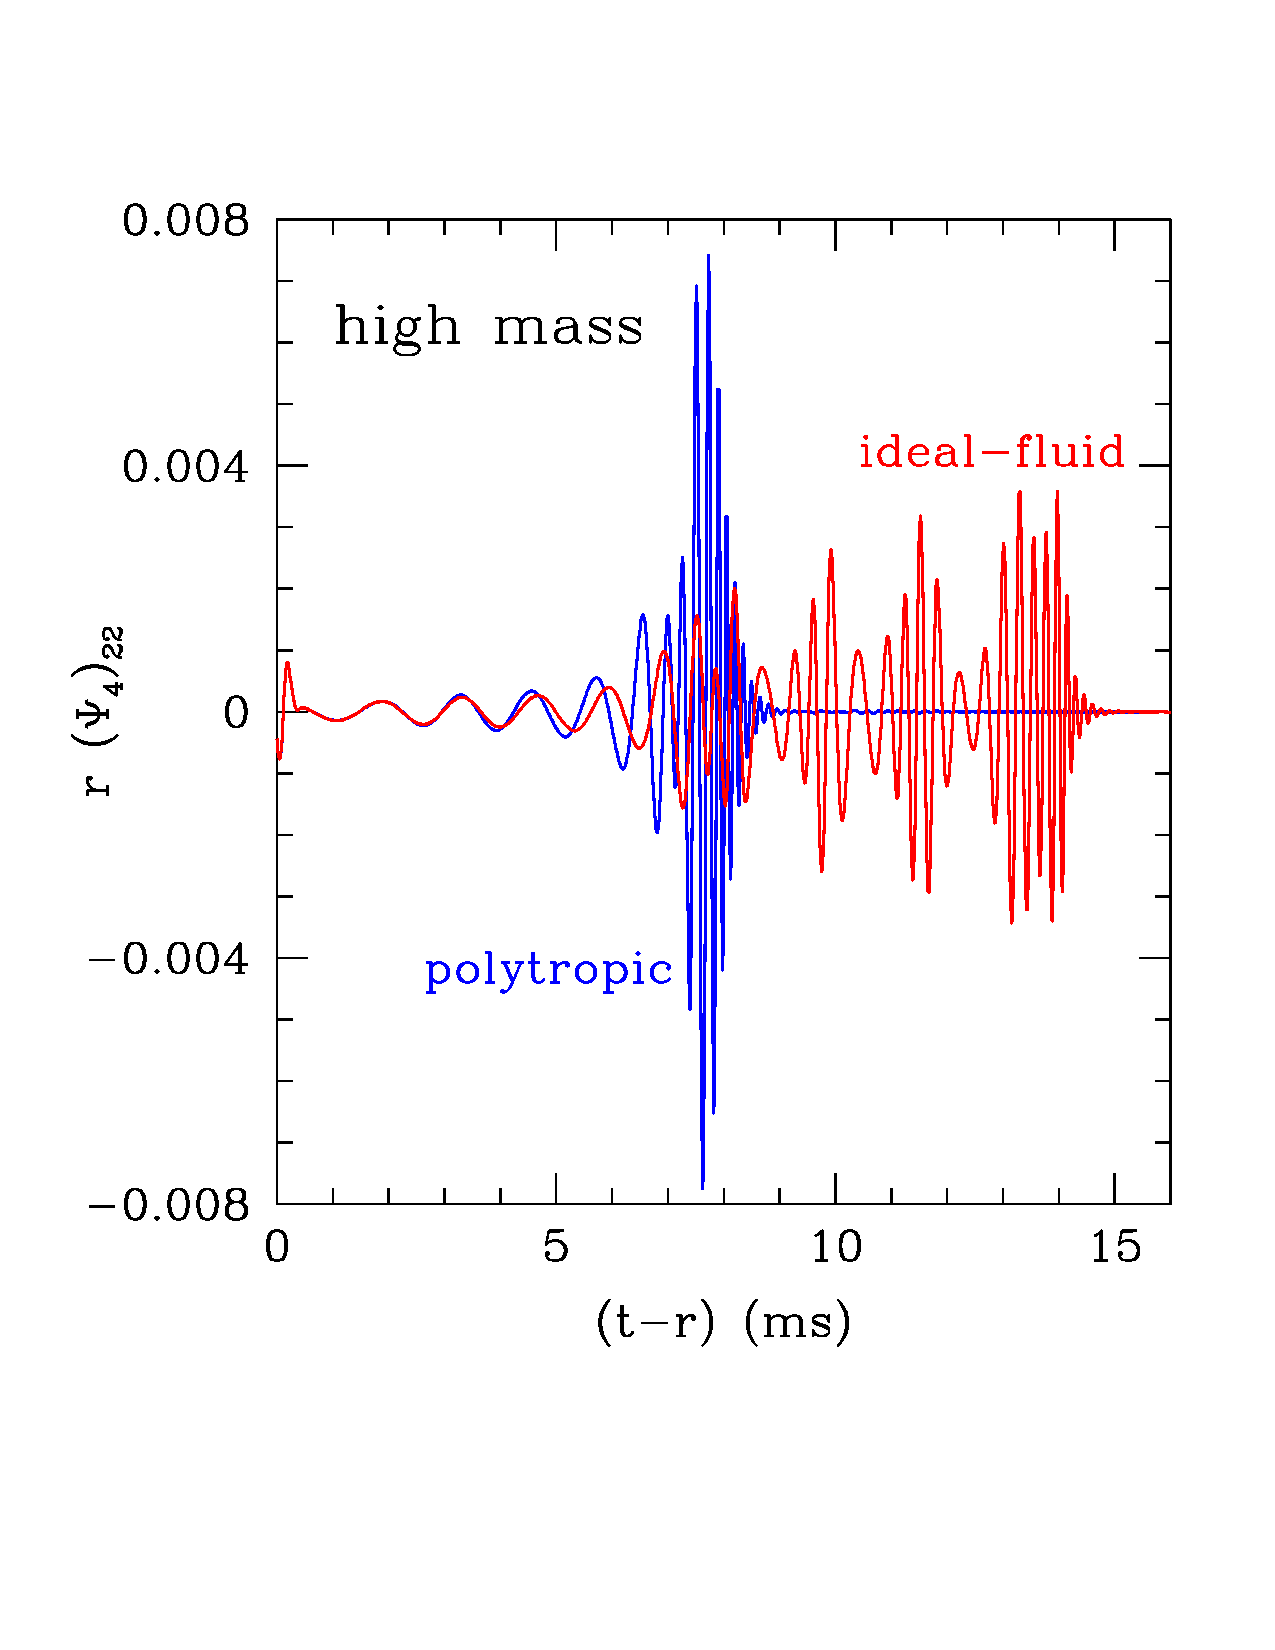
\includegraphics[angle=0,width=0.49\columnwidth]{./Sec_ET_ScienceCase/Psi4_pol_vs_IF_high.pdf}
%\hskip -0.5cm
%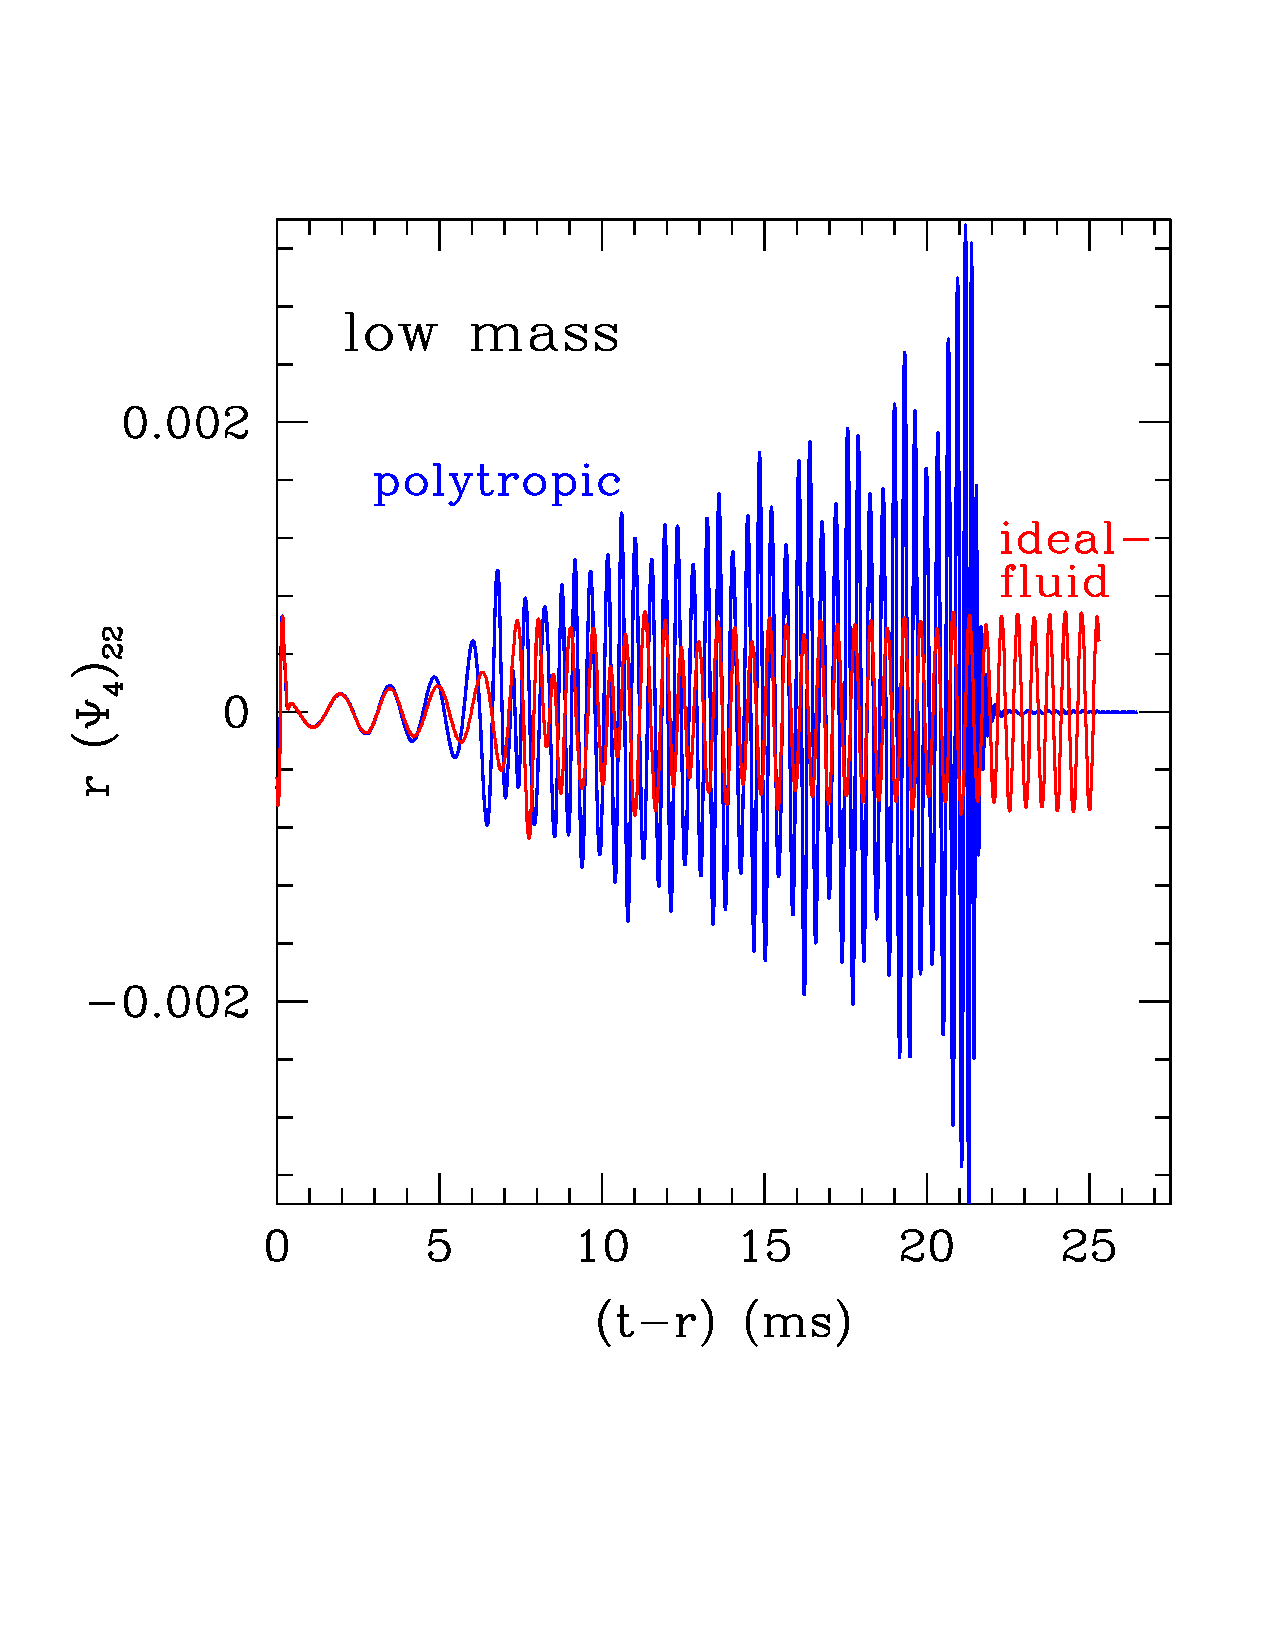
\includegraphics[angle=0,width=0.49\columnwidth]{./Sec_ET_ScienceCase/Psi4_pol_vs_IF_low.pdf}
%\vskip -1.2cm
%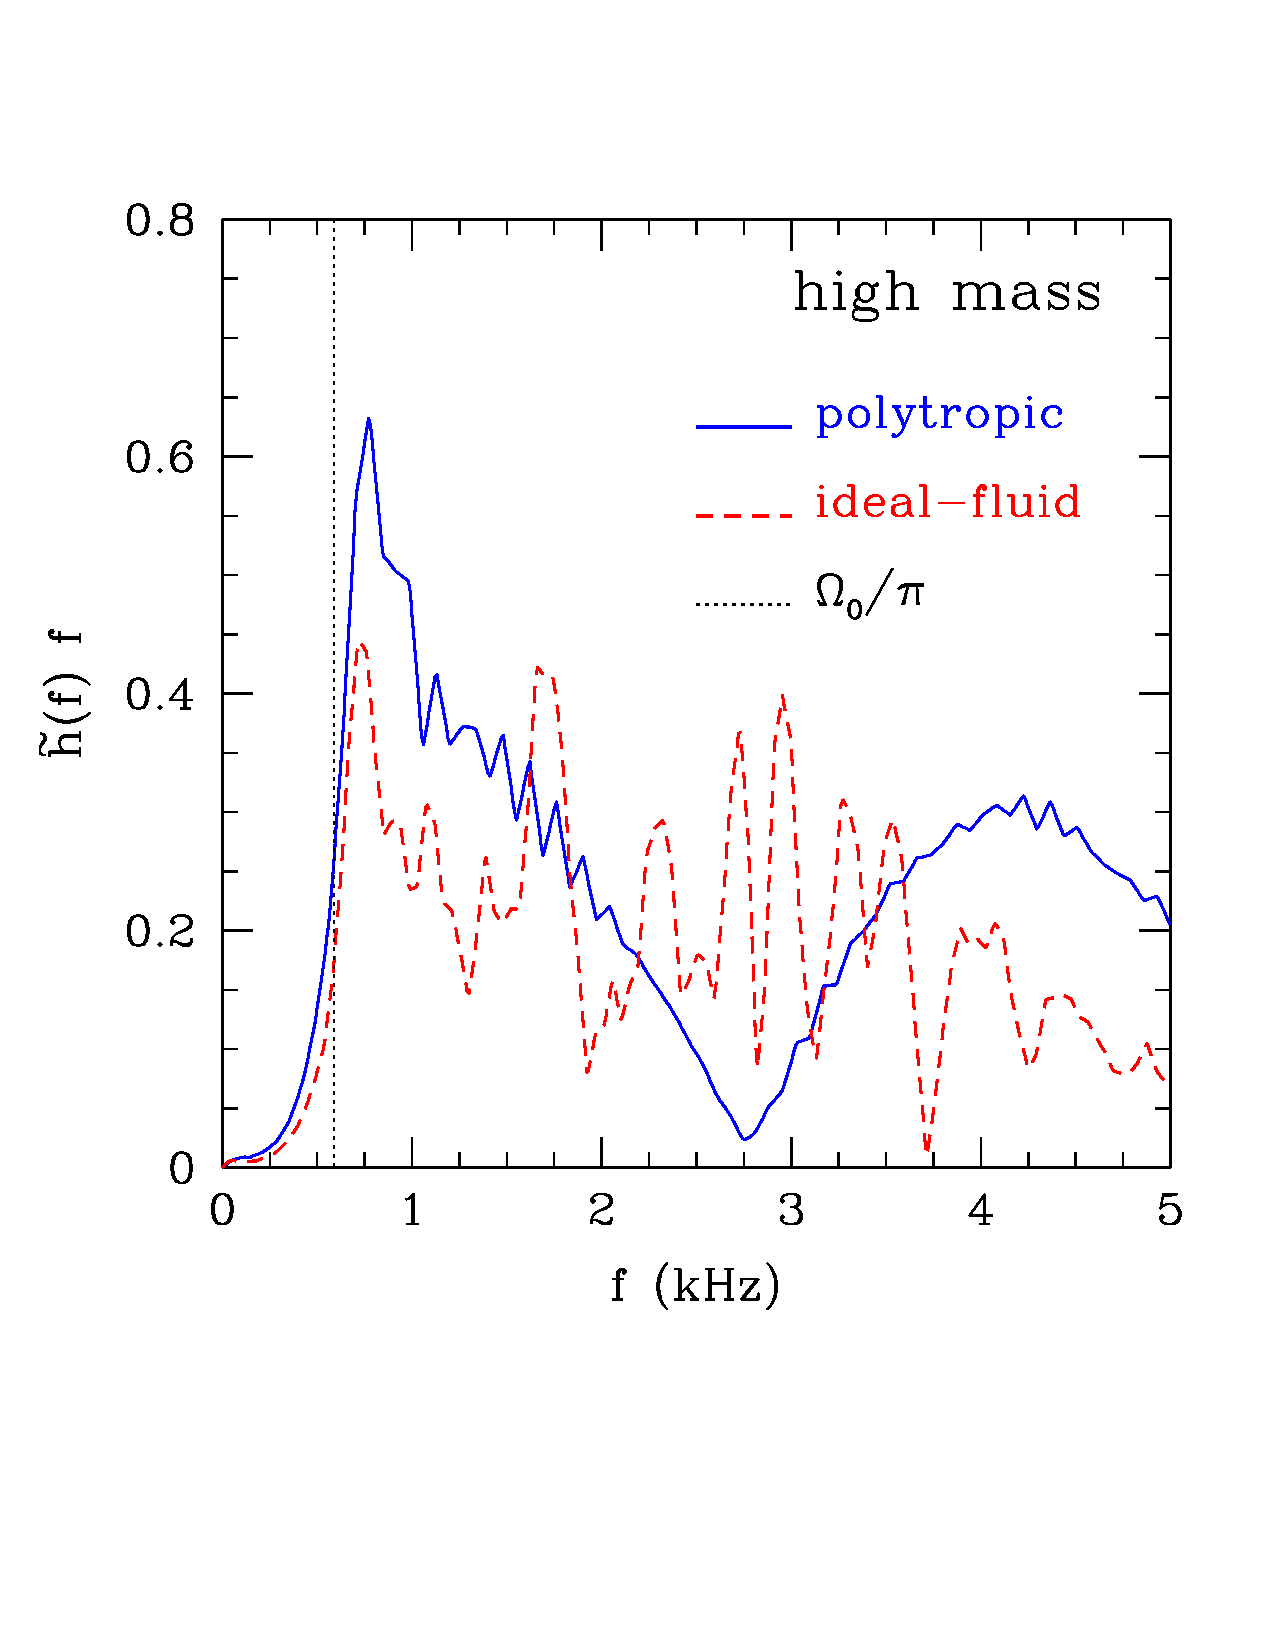
\includegraphics[angle=-0,width=0.45\textwidth]{./Sec_ET_ScienceCase/PSD_h_pol_vs_IF_high.pdf}
%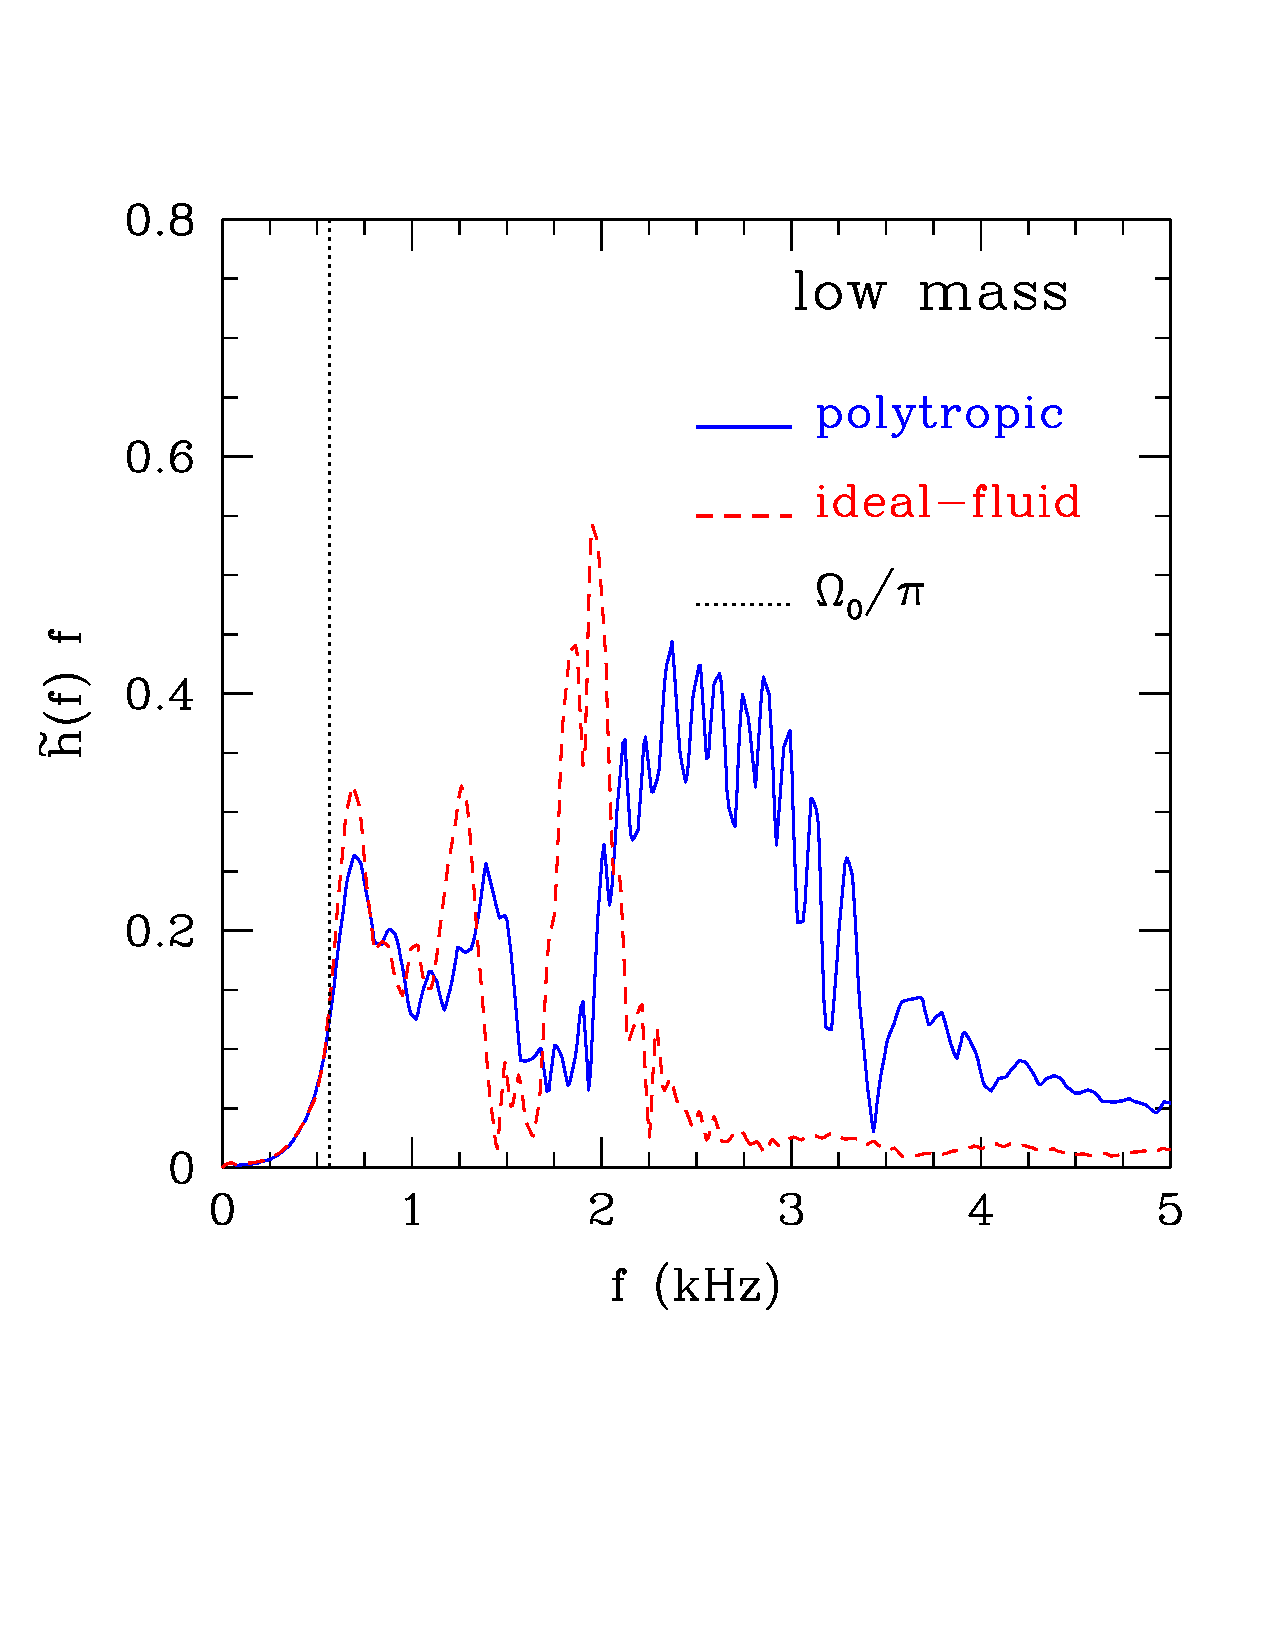
\includegraphics[angle=-0,width=0.45\textwidth]{./Sec_ET_ScienceCase/PSD_h_pol_vs_IF_low.pdf}
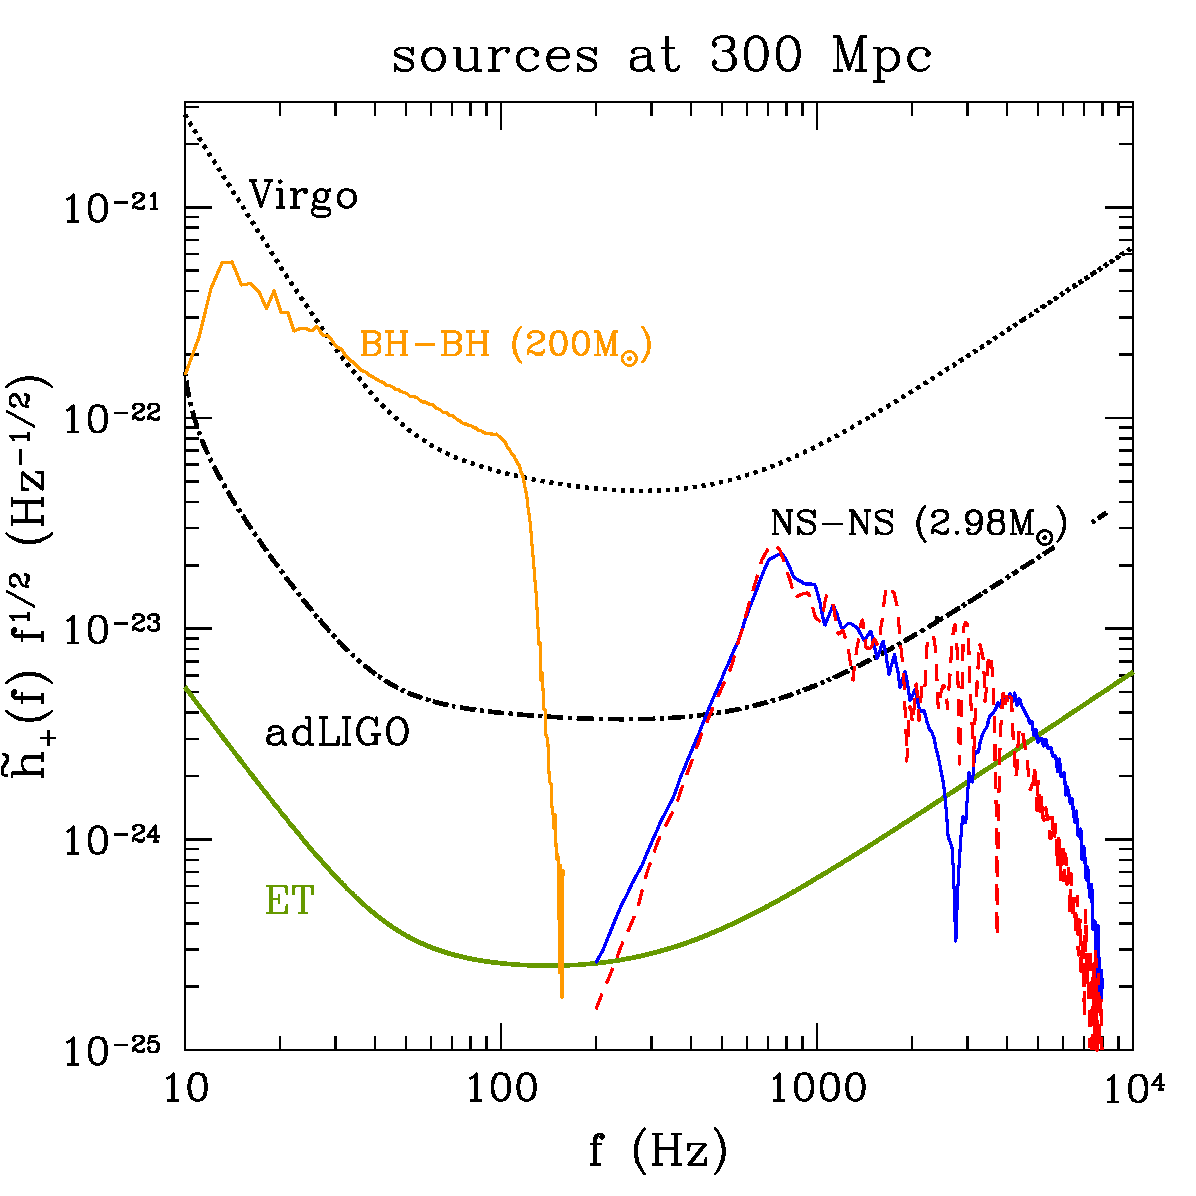
\includegraphics[angle=-0,width=0.45\textwidth]{./Sec_ET_ScienceCase/highmass-NS.pdf}
\hskip 0.2cm
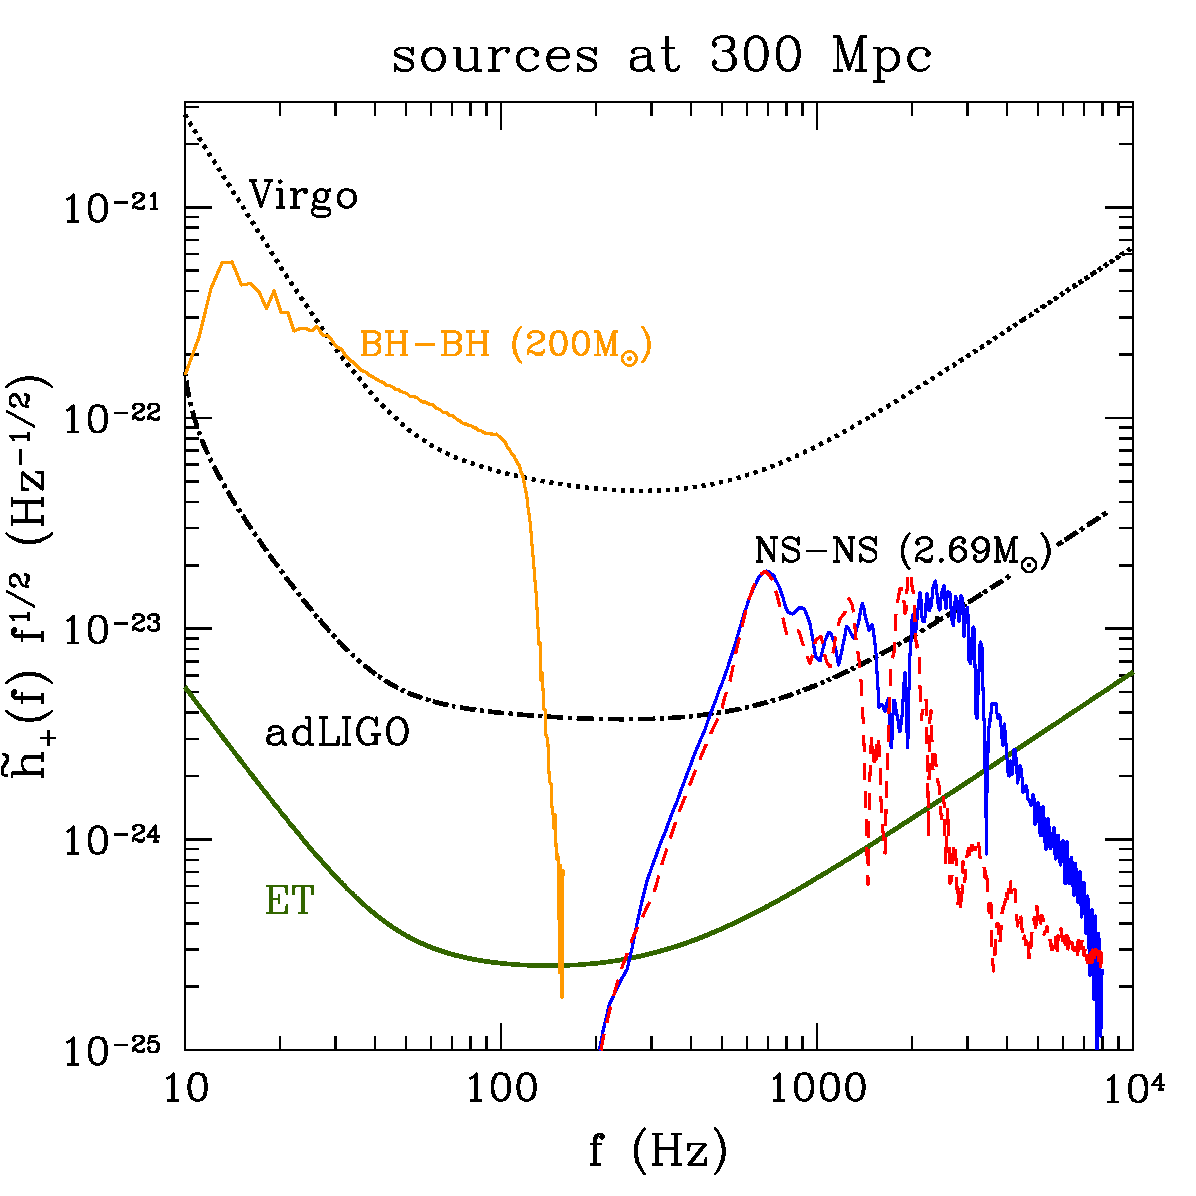
\includegraphics[angle=-0,width=0.45\textwidth]{./Sec_ET_ScienceCase/lowmass-NS.pdf}
\caption{
Gravitational wave spectra of merging neutron star binaries compared to
sensitivities of Virgo, advanced LIGO (labelled adLIGO) and ET. 
Left panel shows spectra of high-mass binaries evolved with the cold 
(blue solid line) or hot (red dashed line) equations of state. Also
shown for comparison is the corresponding spectrum of an equal-mass, 
non-spinning binary black hole with total mass $M=200\,M_\odot,$
which appears in the low-frequency part of the spectrum (orange solid 
line). Right panel is the same as the left panel but for the 
low-mass binary.  It can be seen that the observed spectra are 
sensitive to the neutron star EoS.
%\textit{Top row, left panel:} Comparison of the waveform 
%for a high-mass NS binary (with a total mass of
%$3.2\,M_{\odot}$) when evolved with the a ``cold'' EoS (labeled
%as `polytropic') or with a ``hot'' EoS (labeled `ideal-fluid').
%\textit{Top row, right panel:} The same as in the left
%panel but for a low-mass NS binary (total mass 
%$2.9\,M_{\odot}$). \textit{Bottom row:} The same as in the top
%row but with the comparison being made in frequency
%space with the sensitivity curves of Virgo, advanced LIGO and Virgo
%and ET-B. The source is assumed to be at 300 Mpc.
\label{NS_example}}
\end{center}
\end{figure}

Gravitational waves from binary inspiral and merger are
expected to be frequently observed in ET and the predicted signals have
several interesting EoS-dependent features.
This is illustrated in Fig.\,\ref{NS_example}, based on the simulations
of~\cite{Baiotti08} where a comparison of GW spectra from
BNS mergers is shown together with the noise PSDs of 
Virgo, aLIGO and ET. The panel on the left plots the spectra for 
a system with total mass $2.98\,M_\odot$ while the one on
the right considers a lighter system of total mass $2.69\,M_\odot.$
Both panels show spectra for two different EoS: NSs with the cold EoS 
give rise to two distinct bumps (blue solid lines), the location
and relative heights depending on NS masses. NSs with
the hot EoS exhibit a number of spikes (red dashed lines)
whose detailed structure depends on the NS masses.  
The spectrum of a BBH merger (orange solid lines), on the other 
hand, has no specific feature and is independent of the total
mass of the binary.  While neither of the two equations of state 
considered here are realistic, they span in some sense the extremes 
of the range of possibilities.  Most importantly they show that the 
GW signal from BNS merger will be very sensitive to the mass of 
the stars and their EoS.

While this is especially true in the post-merger phase, the
inspiral phase will also provide important information on the EoS. 
Although for most of the inspiral phase, the component stars of 
a BNS system are well-modeled as point particles, as they approach 
each other, an EoS-dependent tidal deformation modifies their orbits,
changing the late inspiral waveform. The measurability of this effect
in GW detectors can be estimated using both
PN tidal deformation calculations and full numerical
simulations of BNSs with varying EoS. The induced change in the
waveform can be used to measure the radius of the NS quite accurately.

Indeed, the set of numerical simulations of Ref.\,\cite{Read:2009bns} 
show that for a $1.35\, M_{\odot}$--$1.35\, M_{\odot}$
system at $100$\,Mpc ET can measure the radius to within
$\pm 0.5$--$1.0$\,km.  This compares favorably to the range in
predicted radius of roughly 9--16 km.  Parameterizing the variation in
the size of a NS by the pressure at a density of $5\times10^{14}$\,g\,cm$^{-3}$
\cite{Read:2008pp}, gives fractional uncertainty in pressure of 5--10\%.  

%Tidal deformation in NSs is characterized by the parameter 
%$\tilde{\lambda}(m_1,m_2)$ which ranges between $0.5 \times 
%10^{36}$\,g$^2$\,cm$^2$ and $10 \times 10^{36}$\,g$^2$\,cm$^2$ 
%for realistic EoS.  Flanagan and Hinderer 
%\cite{FlanaganHinderer2007} estimate that for a binary at 50\,Mpc
%\begin{itemize}
%\item $\Delta \tilde{\lambda} \sim 1.22 \times 10^{36}$ for $1.35-1.35
%M_\odot$
%\item $\Delta \tilde{\lambda} \sim 1.6 \times 10^{36}$ for $1.45-1.45
%M_\odot$
%\item $\Delta \tilde{\lambda} \sim 1.85 \times 10^{36}$ for $1.35-1.7
%M_\odot$
%\end{itemize}
%for the inspiral phase \emph{below 400\,Hz}. 

The advantage of ET in understanding the NS EoS is not
necessarily the larger number of detections possible with increased
sensitivity, although information about the mass distribution of NS 
populations can also be useful for constrainting the EoS. Instead, ET
will provide very strong signals at reasonable rates; for example two
$1.4\,M_\odot$ NSs inspiralling towards each other within an
effective distance of 100\,Mpc, which is expected roughly once a year,
would give a SNR in ET of over 900.  This makes it possible to precisely
measure the component masses during the early inspiral phase, to detect
small departures from point particle behaviour at moderate
frequencies, and discriminate between merger and post-merger signals
from different models at high frequencies.

An interesting feature that has emerged from studies of BNS
coalescences is the post-merger formation, in some cases, of a
hyper-massive remnant object which oscillates and emits GWs
on fairly long timescales.  The presence or absence of such
post merger oscillations, as well as their characteristic frequency
and duration, varies with the cold EoS. However, they are additionally
sensitive to many physical characteristics such as thermal properties, 
magnetic fields, particle production, and so forth.  The precise details of
the signal are not easy to predict.  However, the signal from such 
a post-merger oscillation should be visible in ET \cite{Shibata2005eos}, 
and analysis of the signal following a measured inspiral phase may provide
useful constraints on the underlying astrophysics.

%It has recently become possible to compute the first complete and
%accurate simulations of the merger of a NS binary through
%to the delayed formation of a BH and its ringdown~\cite{Baiotti08,
%Baiotti:2009gk}. By computing the complete GW signal produced in 
%the process it was possible to show that the emitted signals
%are strongly correlated to the properties of the sources
%emitting them. Differences in the EoS or in the initial mass of the
%system produced different signals with different power spectra and
%different durations.

Furthermore, magnetic fields are commonly present in 
NSs and their possible impact on the dynamics of BNSs
has only begun to be examined.  The effect of magnetic fields on GW
emission during the inspiral and merger of magnetized NSs has 
recently been investigated~\cite{Giacomazzo:2009mp}. It
has been shown that while initial fields of strength 
$B_{0}\gtrsim 10^{12}\,{\rm G}$ have an impact after the merger,
fields of sufficiently strong strength $B_{0}\gtrsim 10^{16}\,{\rm G}$
will affect the inspiral phase too.
%These results are quantified by computing the
%overlap between the waveforms produced during the inspiral by
%magnetized and unmagnetized binaries. 
ET provides a strong impetus for such theoretical studies.  By 
including more realistic equations of state and realistic radiation 
transport schemes, it will be possible to considerably increase our 
level of understanding of these objects. 

\FloatBarrier
\subsubsection{Neutron star physics from pulsar glitches}

% \ledby{Glampedakis}
Many radio pulsars exhibit {\em glitches,} events in which 
a NS is seen to suddenly spin-up, followed by a relaxation period towards
stable secular spin-down. Pulsar glitches have a long observational 
history (beginning shortly after the discovery of the first pulsar)
\cite{Anderson:1975}. 
So far, over a hundred pulsars are known to have glitched at least once
(for a recent survey, see, Ref.\,\cite{Espinoza:2011pq}).
Glitches have also been observed in magnetars --- highly magnetized NSs.
The archetypal glitching pulsar is Vela, which exhibits regular
large glitches with an amplitude corresponding to a fractional spin 
frequency change of the order of $10^{-6}$\,\cite{Ruderman:1976}.

Despite the wealth of observational data, the glitch
remains an enigma from a theoretical point of view \cite{McDonald:2007}. 
It is widely 
believed that glitches are related to the existence of superfluids 
in the interior of mature NSs and that they involve a transfer 
of angular momentum from a superfluid component to the rest of the 
star which includes the crust (to which the pulsar mechanism is presumed 
to be rigidly attached) and the charged matter in the 
core \cite{Anderson:1975, McDonald:2007}.  Key to this idea is the fact that 
a superfluid rotates by forming an array of quantized vortices. 
In essence, the superfluid can spin down only if
the vortices can move outwards.  If the vortex motion 
is impeded by `pinning' to the other component, e.g. the crust nuclei, 
then the superfluid 
cannot keep up with the spin-down due to electromagnetic braking. 
As a result a rotational lag develops between the two components,
until some critical level is reached at which the vortices unpin and 
transfer angular momentum to the rest of the star, and the two 
components are driven to corotation.

Taking the basic two-component picture at face value,  one can estimate 
the available energy that may be radiated at a glitch event. This 
suggests that large Vela glitches may release an energy of the order 
of  $ 10^{42}$~erg ($10^{-12}\,M_\odot$). This is a useful estimate 
as it provides an idea of how energetic regular neutron star events in 
our galaxy may be.  Of course, one must keep in mind that this 
energy may not be associated with GW emission at all. This depends 
on the detailed glitch mechanism, e.g. the asymmetries involved. 
From a general point of view, on would expect glitches originating 
in the star's crust to be associated with very weak GWs (the involved 
densities are simply too low to be relevant). As the standard glitch 
scenario is associated with vortex pinning to crust nuclei, this 
would rule out these events are interesting GW sources. However, 
there is some evidence that the largest observed glitches may require 
the fluid core to be involved (e.g. through pinning of vortices to 
superconducting fluxtubes). This may change the situation dramatically, 
as the denser regions of the star are now involved. It also hints at 
the interesting possibility that the observed phenomenon could be the 
``tip of the iceberg'', reflecting more energetic dynamics in the 
fluid core. This is, of course, speculative but it is relevant to 
note that the level of sensitive of ET may set strong upper limits 
on the possible scenarios. Translating the rough energy estimate into 
a GW amplitude, by assuming that the energy is released through the 
f-mode (a frequency of 2~kHz lasting for a fraction of a ms at a 
distance of 10~kpc) we find an effective amplitude around 
$10^{-23}$. (This estimate assumes we can do matched filtering, which 
is relatively easy for these damped sinusoids.) A signal of this 
strength should be within the reach of ET.  An observed signal  
would immediately constrain the cold-matter nuclear 
EoS\,\cite{AnderssonKokkotas1998, Living:AnderssonComer}. A lack of 
detection would set relevant limits on the asymmetry and fluid 
dynamics associated with pulsar glitches.  
%[CHECK MELATOS]

In order to do better than these rough estimates we need to improve 
our understanding of superfluid hydrodynamics and possible 
instabilities leading to glitches.  There has been some recent 
progress on this, and it seems reasonable to expect the theory to 
have developed significantly by the time of ET construction. There 
has been particular progress on the issue of the origin of the 
glitches, e.g. the instability that triggers large-scale vortex 
unpinning. A recent model suggests that the glitch trigger-mechanism 
may be the result of a superfluid  ``two-stream'' instability 
setting in through the inertial modes of the system 
\cite{Andersson:2002dv,Andersson:2002zd}. However, in this model 
the unstable modes have very short wavelengths and would not be 
effective GW emitters. Whether the idea can be developed into a 
more complete scenario remains to be seen.

Regardless of the theory uncertainties, an instrument like ET would 
be ideal for detecting a GW signal in the 10--100\,Hz band, which 
would be the relevant for the inertial modes of a Vela-like pulsar. 
The detection of GW signals from glitching pulsars would provide a 
tool for probing the interior matter of NSs and supplement EM 
observations.  The realisation of this exciting prospect will require 
(as in the case of other potential sources of gravitational radiation) 
the input of theoretical waveform templates. These waveforms need to 
be computed using detailed multifluid hydrodynamical models for 
superfluid NSs, accounting for effects like vortex mutual friction 
and pinning.

\FloatBarrier
\subsubsection{GW from the r-mode instability}

% \ledby{Leone B. Bosi}

Neutron stars may suffer a number of instabilities. These instabilities 
come in different flavours, but they can all be directly associated 
with unstable modes of oscillation \cite{Andersson:2003}.
A study of the stability properties of a relativistic star is thus 
closely related to an investigation of the star's various pulsation 
modes.  Furthermore, non-axisymmetric stellar oscillations will 
inevitably lead to the production of gravitational radiation.  
Detection of these signals would allows us to  put constraints on 
the interior structure of the star and the extreme physics associated 
with the high-density region.

The most promising instability scenarios concerns rotating stars.  
Of particular interest are the GW driven instabilities of the 
f-modes and the r-modes.  The action of the former is to deform 
the star into a bar-shape, which is an ideal GW emitter.  Meanwhile, 
the r-mode radiate predominantly through the current multipoles. 
The radiation mechanisms are rather different, but the issues 
involved in studying these instabilities are very much the same.  
First we need to establish that the modes can become unstable in 
a realistic neutron star.  This means that the GW driven growth 
must overcome the relevant dissipative damping mechanisms.  We 
need to consider the (standard) shear- and bulk viscosities, and 
understand how the associated rates depend ion the star's 
composition. We also need to consider more exotic mechanisms, e.g. 
strong bulk viscosity associated with hyperon reaction and vortex 
mediated friction in a superfluid mixture. Significant effort has 
gone into these problems in the last decades.  The current 
understanding is that the instability of the r-modes is likely to 
be the most relevant, but scenarios associated with the  unstable 
f-modes should definitely not be ruled out. Basically, the threshold 
for the r-mode instability to set in in a mature neutron star is 
a relatively low fraction of the break-up rotation rate. Meanwhile, 
the f-mode become unstable only near the break-up limit.  Moreover, 
the f-mode instability is thought to be completely suppressed in a 
superfluid neutron star (due to the vortex mutual friction).  This 
is not the case for the r-modes, which are not dominated by this 
mechanism. 

However, detailed modelling suggests that the r-modes reach nonlinear 
saturation at relatively low amplitudes. This limits the GW emission. 
The underlying mechanism, the coupling of the r-mode to a large 
number of short wavelength inertial modes, also leads to the GW 
signal being immensely complex (leading to difficulties to carry 
out matched filtering). Having said that, the best current estimates 
suggest that the r-mode signals should be detectable from systems 
in our galaxy (and slightly beyond) \cite{Bondarescu:2009}.  The 
detectability of the f-modes may be more favourable. In particular, 
recent work shows that the growth time of the f-mode instability 
may be extremely short. However, it is not known if the f-mode 
instability saturates at low amplitudes. If it does not, then the 
associated signals may be detectable from the Virgo cluster. This 
would increase the event rate which would counter the fact that 
we need a very fast spinning neutron star at birth for the mechanism 
to operate.  Further theory progress is needed to make more precise 
statements. What is undoubtedly clear is that, if these GW signals 
are at a level that would be detectable by second generation 
detectors (as suggested) then ET will provide a supreme instrument 
for extracting the relevant physics information. This is a 
tremendously exciting prospect, given the dependence on interior 
neutron star physics that is very difficult to probe by other means.

\paragraph{The strength of gravitational waves from r-modes}
In order to estimate the GW signal associated with the unstable 
r-modes, let us make use of a simple phenomenological model. 
The model accounts for the differential rotation induced by 
the modes~\cite{SaTome}, but does not account for much of the 
complicated core physics considered in other work.  Nevertheless, 
the estimates provide a useful guide to the relevance of these 
GW signals.  Thus detection of such GWs is more difficult than 
initially supposed. In the model, the amount of differential 
rotation is described by a parameter $K$, which encodes the 
level of differential rotation and which may take values in 
the range $[-5/4, 10^{13}]$ depending on the initial conditions.

The detectability of GW produced by r-modes depends upon the 
amount of angular momentum that they carry away. As described 
in \cite{SaTome1}, for $K=0$, the total angular momentum of 
the star decreases to $65\%$ of its initial value, and 
part of the initial angular momentum of the star, about $58\%$, 
is transferred to the r-mode as a consequence of the rapid 
increase of the average differential rotation. Therefore the 
initial angular momentum carried away by gravitational waves 
is about $35\%$. This result is strongly dependent on the value 
of $K$: for higher $K$ the amount of angular momentum carried 
away by gravitational waves may even fall below $1\%$.

\begin{wrapfigure}{l}{0.5\textwidth}
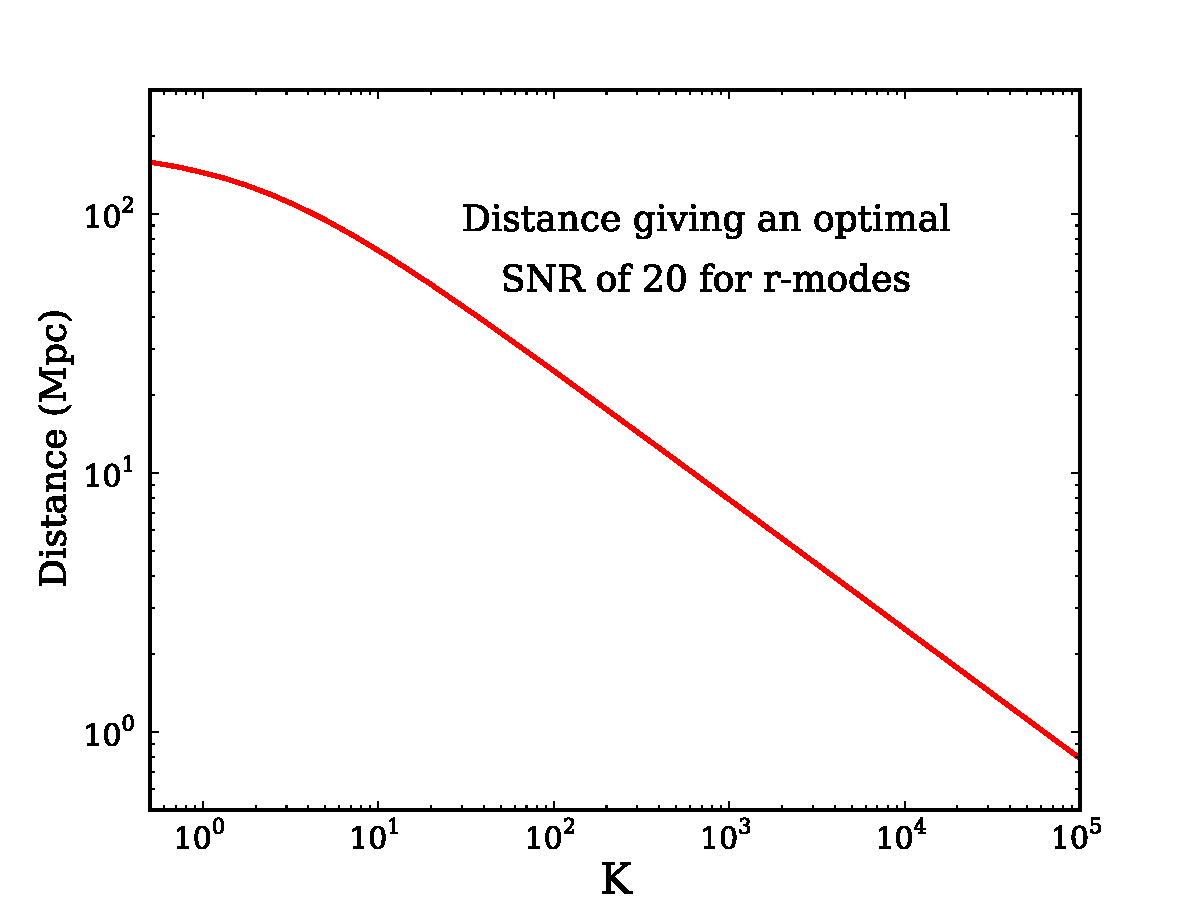
\includegraphics[width=0.5\textwidth]{./Sec_ET_ScienceCase/Rmodes_redone.pdf}
\caption{Detectability of r-modes expected in 
Einstein Telescope (ET-B sensitivity) as a function of the $K$ parameter
describing the strength of differential rotation.}
\label{fig:RmodesVsET}
\end{wrapfigure}
%
In the case of the r-modes, the frequency $f$ of the GWs
depends on the NS's angular velocity $\Omega$ as $f=2\Omega/(3\pi)$. 
The frequency range is estimated as follows:
$f_{min} \simeq [77-80]\,$Hz, depending on the final value 
of the angular velocity $\Omega (t_f)$ and $K$;
$f_{max} \simeq 1200\,$Hz, depending on the initial value 
of the angular velocity $\Omega _0$.
The amplitude in the frequency domain is given by:
\begin{equation}
H(f)=\frac{4.6\times10^{-25}}{\sqrt{2+K}}
\sqrt{\frac{f_{max}}{f}}\frac{20\,{\rm Mpc}}{D}\,{\rm Hz}^{-1}
\end{equation}
where $D$ is the source distance, $f$ the GW signal frequency 
and $f_{max}=1191\,$Hz is its maximum frequency.

We may estimate the signal to noise ratio (SNR) at ET by adapting 
a calculation made for Advanced LIGO in \cite {SaTome1}\footnote{The 
sensitivity curve used for our estimation is ET-B.}. The optimal 
SNR is given by
\begin{equation}
\frac{S}{N}=\frac{250}{\sqrt{(2+K)}}\frac{20\,{\rm Mpc}}{D}.
\end{equation}
The strong dependence on the unknown parameter $K$ is clear, as 
shown in Figure~\ref{fig:RmodesVsET} where we consider an SNR 
of 20, arbitrarily chosen for a confident observation of the 
signal. This dependence provides a useful illustration of the current uncertainties 
associated with r-mode signals. On the one hand, it may be 
that the distance
at which a GW signal could be visible with ET is really large. Considering 
the optimistic case when $K$ approaches zero, we obtain a horizon 
distance for an optimally oriented source of $175\,$Mpc. However, 
in the less optimal case when $K=[10^{5}-10^{6}]$, the 
horizon falls to less than $1\,$Mpc (galactic sources). The latter 
range agrees quite well with the most realistic models, where the 
r-mode evolution is determined by nonlinear mode-coupling \cite{Bondarescu:2009}.
Significant uncertainties remain, as all current models are somewhat incomplete, but 
there is every reason to expect that our understanding of the 
physics would have improved considerably by the time ET comes into operation.
Improvements are certainly necessary if we want to be able to carry out
an optimal search for these signals. Still, the current evidence of the astrophysical 
relevance of the r-modes makes this a very promising target 
for ET (see Box \ref{box:rmodes}).


\etbox{r}{box:rmodes}
{R-modes and ET science goals}
{
A significant motivation for studying GWs from the r-mode instability 
with ET is the opportunity to obtain a unique correlation with the nuclear 
physics and astrophysical scenarios involving NSs, ranging from their 
birth following supernovae to the spin evolution of accreting NS in LMXBs. 
The signal could provide a fundamental probe of NS dynamics. Some possible 
implications are given below:
\begin{itemize}
\item In principle from GW signals and signal models it is possible 
to trace and quantify the initial conditions of the new-born star 
such as initial frequency, initial temperature and others. This could 
lead to the confirmation or exclusion of supernova models, star 
formation processes and NS models.
\item Another implication concerns NS nuclear physics models and 
the EoS, potentially opening a window on the core and crust physics, 
especially superfluid aspects.
\item The phenomenon of NS cooling due to neutron emission also 
interacts with the r-mode instability. In this case GWs could 
provide information about the cooling rate and cooling model, 
which at the moment is assumed to follow the modified URCA process.
\item GWs emitted by accreting NS in LMXBs may limit the attainable rotation rate. 
Evidence for this would solve a long standing puzzle concerning the absence of 
extremely fast rotating pulsars. 
\end{itemize}
}

\FloatBarrier
\subsubsection{Solving the enigma of GRB progenitors}


% \ledby{O'Shaughnessy, Jones, Clark}
\label{sec:grb_progenitors}

Gamma-ray bursts (GRBs) are the most luminous explosions in the universe\footnote{
Gravitational waves from merging BHs will be many orders of mangitude more
luminous but until they are detected GRBs will remain the most luminous events
in the Universe.}.
Through observations made by satellite-based gamma-ray observatories it was found
that the duration of the GRBs follows a bimodal distribution
\cite{Kouveliotou:1993}.
GRBs are classified either as \emph{short-hard} or \emph{long-soft} bursts depending
on their duration and spectra.
Through follow-up observations of the  x-ray, optical and radio afterglow emission of
GRBs it is possible to determine their sky location, redshift and host galaxy.

\paragraph{Long and short GRBs}
Long GRBs are always associated with late-type star-forming host galaxies
\cite{conselice05}.
A handful of long GRBs have also been associated with supernovae
\cite{galama98,kulkarni98,Hjorth2003,Campana:2006qe}.
It is therefore thought that core-collapse supernovae are the progenitor of long
GRBs \cite{woosley93,iwamoto98}.

Short GRBs are observed at lower redshifts than long GRBs and are associated with a
variety of galaxy types including early-type elliptical and lenticular galaxies
without active star forming regions \cite{bloom-2006}.
Currently, it is widely thought that merger of BNS or
NSBH systems are the progenitors of most short-hard GRBs
\cite{bloom07}.
Some small fraction of short GRBs (less than $15\%$ of known short GRBs) may
be caused by soft gamma repeater flares (SGRs)~\cite{2006ApJ...640..849N,Chapman:2009}.
SGRs are described later in this section.

As discussed in \ref{sec:binaries}, accurate predictions for the GW emission of the
inspiral, merger and ringdown of compact binaries are possible through
post-Newtonian approximations to Einstein's equations or through numerical
relativity simulations. Therefore, it is possible to employ pattern matching
techniques such as matched filtering to extract these signals from noisy data.
GWs from inspiralling binaries have been searched using matched-filtering
in data from initial interferometers (LIGO, Virgo, GEO) 
(see, e.g., \cite{Abbott:2003pj,Abbott:2005pe}.  A search GW in coincidence 
with short GRB 070201, whose sky-location error box overlaps the spiral arms 
of M31, excluded an inspiral progenitor if it was indeed located in 
M31 with a confidence of $99\%$ \cite{LSC:GRB070201}.
Figure~\ref{fig:ET_range} shows the horizon distance for
ET, where the figure for BNS with $m_{\rm NS} = 1.4\, M_{\odot}$ 
can be read off for a total mass $2.8\,M_{\odot}$ and spin parameter 
$\chi=0$ to be about $17\,\rm Gpc.$ For NSBH systems, the distance
reach is $z\sim 2$-5 depending on the total mass of the system.
Since short GRBs are mostly found at lower red-shifts ($z<1$), ET 
will observe almost all of them assuming they are indeed progenitors
of binary neutron star mergers.

Predicting the GW emission of core-collapse supernovae associated
with long GRBs is more difficult and involves modelling the complicated 
internal dynamics of the collapsing star---see \emph{e.g.}\ \cite{ott:09}.
Searches for unmodelled gravitational emission from GRBs
on data from initial interferometers (LIGO, Virgo, GEO) have also been
carried out \cite{LSC:GRB070201, LSC:S5GRBBurst}. The sensitivity of
such searches can be determined as follows:
The amplitude of a gravitational-wave burst can be characterized by
the root-sum-square amplitude $h_{\rm rss}$ via
\begin{equation}
h_{\rm rss} = \sqrt{\int (|h_+(t)|^2 + |h_\times(t)|^2) \, dt} \,.
\label{eq:hrss}
\end{equation}
Coherent search analysis techniques \cite{LSC:S5GRBBurst} can detect 
generic bursts at 90\%-confidence an amplitude $h_{\rm rss}$ of
around an ten times the amplitude spectrum of an interferometer, 
i.e.\  they can detect a signal if it produces $h_{\rm rss}^{\rm min} \sim 
10 \times S_{h}(f)^{0.5}$.  For narrow-band burst signals we can 
use the following approximation for the energy in GW for a given
$h_{\rm rss}$:
\begin{equation}
E^{\rm iso}_{\rm GW} \simeq \frac{\pi^2 c^3}{G} D^2 f_{0}^{2} h_{\rm rss}^{2},
\end{equation}
where $E^{\rm iso}_{\rm GW}$ is the isotropic energy emission in GWs,
$D$ is the distance of the source and $f_0$ is the central frequency. 
From Eq.~\ref{eq:hrss} we can calculate a lower limit on source distance from
the minimum amplitude $h_{\rm rss}^{\rm min}$ for a given value of 
$E^{\rm iso}_{\rm GW}$.
For long GRBs the energy of emission in GWs is not well known
but has been estimated to be as high as $0.2\, M_{\odot} c^2$ in the LIGO-Virgo
frequency band of good sensitivity \cite{vanPutten:grb} but it could be
$0.001\,M_\odot c^2$ \cite{davies:2002,king:2005,piro:07} or even lower.
In Fig.~\ref{fig:distanceFreq_5percentMsol} we estimate the distance to which
various detectors are sensitive to a narrow-band burst of GWs
assuming $E^{\rm iso}_{\rm GW} = 0.05 M_{\odot} c^2$.
Clearly, ET has a distance reach of $z>1$ for long GRBs~\cite{springerlink:10.1007/s10714-010-1019-z} if
the energetics are favourable and could be used as a testbed for
different astrophysical models.

\paragraph*{Soft Gamma Repeater Flares}
% \ledby{Clark}
\label{sec:SGR}

As described above, a significant fraction, up to $15\%$, of short, hard GRBs may be associated with flaring activity in soft gamma-repeaters (SGRs).  These sources often undergo sporadic periods of activity which last from days to months where they emit short bursts of hard X-rays and soft $\gamma$-rays with luminosities $L\sim 10^{41}$\,erg\,s$^{-1}$ and photon energies in the range $10\mbox{--}30$\,keV.  Much more occasionally, they exhibit enormous, giant flares with luminosities as large as $10^{47}$\,erg\,s$^{-1}$.  There are 4 known soft $\gamma$-repeaters: three in the Galaxy and one in the Large Magellanic Cloud. It is generally believed that SGRs belong to a class of NS, magnetars, with extraordinarily large magnetic fields in the range $10^{14}\mbox{--}10^{15}$\,G where the flaring activity is due to sudden, violent reconfigurations of complex magnetic field topologies.

The hardness of their spectra and the enormous luminosities involved mean that giant flares from nearby SGRs, such as that of SGR 1806-20~\cite{Hurley:2005}, represent an intriguing candidate progenitor scenario for some short duration $\gamma$-ray bursts.  Indeed, in Ref.\,\cite{Tanvir:2005}, the authors report a correlation between the positions of some short GRBs with those of low redshift galaxies, suggesting that $10-25\%$ of short GRBs occur in the local universe and, therefore, are likely to be associated with giant SGR flares.  Furthermore, evidence for the existence of two classes of progenitors for short GRBs is provided in Ref.\,\cite{Chapman:2009}.  Here, it is found that a bimodal luminosity function, representing a dual-population of short GRB progenitors with low and high luminosities, is required to reproduce the observed distributions of short GRB luminosities.  As well as statistical evidence, there have been observations of at least three individual short GRBs which present candidates for 
extragalactic SGR flares.
%\begin{figure}[tbp]
%\begin{center}
%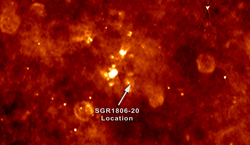
\includegraphics[width=0.49\textwidth]{./Sec_ET_ScienceCase/SGR1806_Radio_LocationArrow.jpg}
%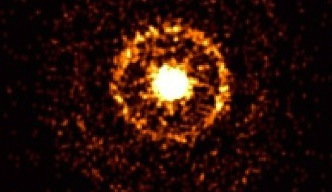
\includegraphics[width=0.49\textwidth]{./Sec_ET_ScienceCase/SwiftRing.jpg}
%\caption{Left: A high resolution, wide-field image of the area around SGR1806-20 as seen in radio wavelengths. SGR1806-20 cannot be seen in this image generated from earlier radio data taken when the source was ``radio quiet''. The arrow locates the position of SGR1806-20 within the image. Credit: University of Hawaii.
%Right: Swift's X-Ray Telescope captured an apparent expanding halo around the flaring NS SGR J1550-5418. The halo formed as X-rays from the brightest flares scattered off intervening dust clouds. Credit: NASA/Swift/Jules Halpern, Columbia University.}
%\end{center}
%\end{figure}

Optical and infrared observations~\cite{Levan:2008} of GRB 050906 suggest a tentative association with the local, fairly massive ($M\sim 10^{11}M_{\odot}$) starburst galaxy IC328 which lies at a redshift of $z=0.031$.  If GRB 050906 had indeed originated in IC328, the isotropic equivalent energy would be $E_{\rm ISO}\sim 1.5 \times 10^{46}$\,erg in the 15--150\,keV range.  The giant flare from SGR~1806-20, by comparision,  emitted $E_{\rm ISO}\sim 4\times 10^{46}$\,erg with photon energies $>30$\,keV.  As well as the potential similarity in the energetics of this burst, the association with a starburst galaxy, where young, shortly lived magnetars are believed to be most prevalent, corroborates the SGR progenitor scenario.  

Two other short GRB-SGR flare candidates, GRB 051103 and GRB 070201, were detected by the Konus-Wind GRB spectrometer~\cite{Frederiks:2008,Ofek:2008}.  The localisation area of GRB 051103 was found to lie near M81 (3.6\,Mpc), suggesting an isotropic equivalent energy $E_{\rm ISO}=7\times 10^{46}$\,erg.  As remarked in~\cite{Frederiks:2008}, if GRB 051103 was \emph{not} related to an SGR flare, we would expect an optical and/or transient in the localisation area, which has not been observed.  Finally, the localisation area of GRB 070201 was found to overlap with the spiral arms of M31 ($0.78$\,Mpc), leading to an estimate of $E_{\rm ISO}\sim 1.5\times 10^{45}$\,erg under the SGR flare scenario, again comparable to the giant flare from SGR~1806-20.

In addition to these types of arguments related to the energetics of the EM emission, GW observations can provide an extremely powerful tool to identify SGRs as short GRB progenitors.  First, we note that the failure to detect the signature of a compact binary coalescence from short GRBs at distances where such a signal is expected can provide compelling evidence for the SGR progenitor scenario alone.  Indeed, observations by the initial LIGO instruments recently excluded the coalescence of a binary NS system within M31 at more than $99\%$ confidence as the progenitor for GRB 070201~\cite{LSC:GRB070201}.  Furthermore, a BNS merger is excluded at distances less than 3.5\,Mpc with $90\%$ confidence.  If, however, the progenitor had been an SGR flare, the LIGO observations imply an upper bound on the isotropic energy released as an unmodeled GW burst of $E_{\rm ISO}^{\rm GW}< 7.5 \times 10^{50}$\,erg, within the bounds permitted by existing models.

\begin{figure}[tbp]
\begin{center}
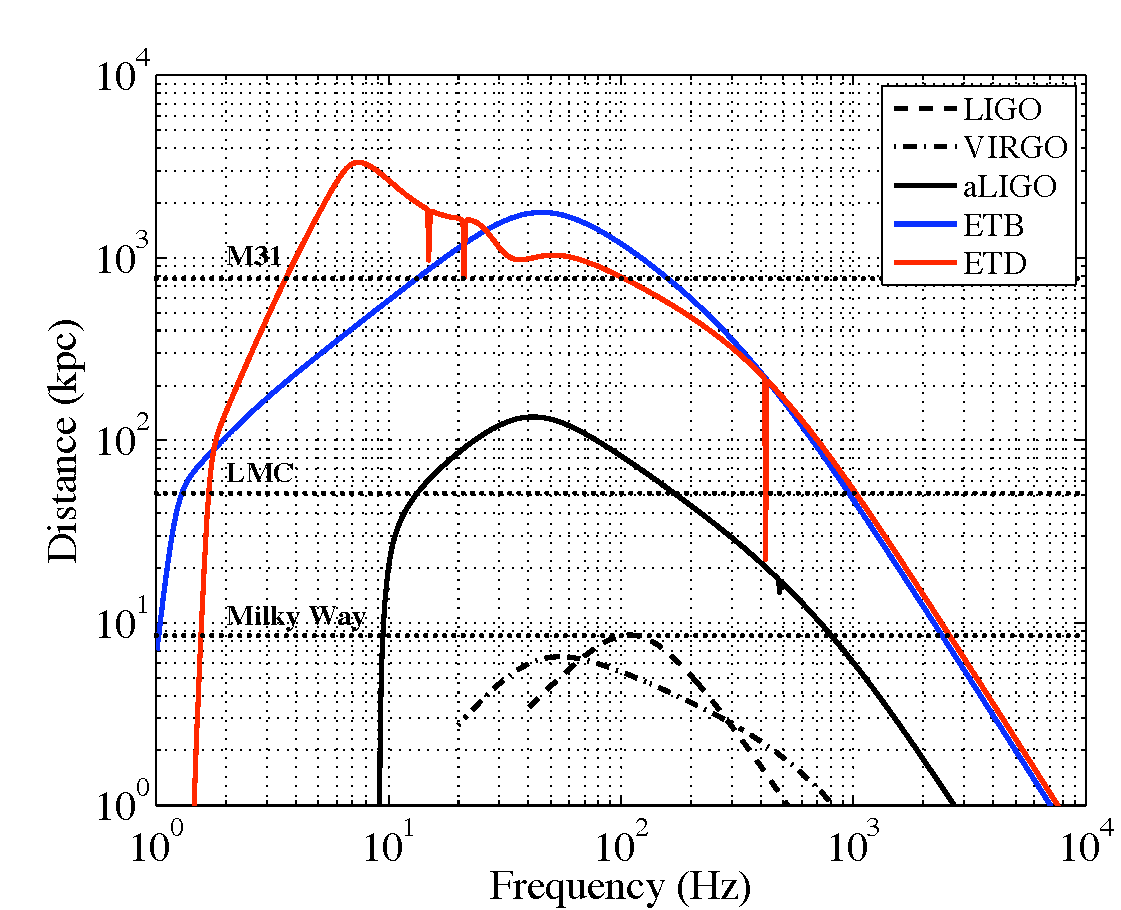
\includegraphics[angle=0,width=0.45\columnwidth]{./Sec_ET_ScienceCase/SGR_distance.pdf}
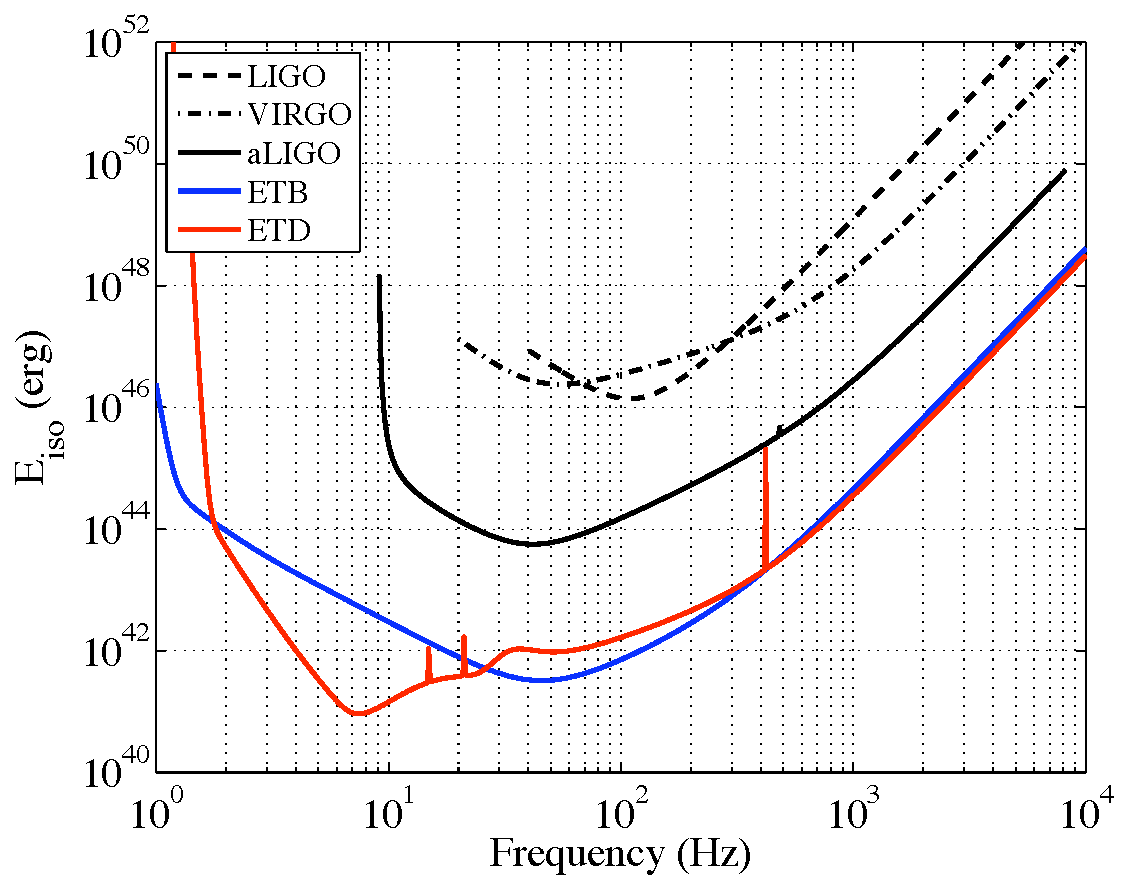
\includegraphics[angle=0,width=0.45\columnwidth]{./Sec_ET_ScienceCase/SGR_energy.pdf}
\caption{\emph{Left panel}: 90\%-confidence lower limit on distance for burst sources assuming $E^{\rm iso}_{\rm GW} = 10^{46} {\rm ergs}$ for an SGR progenitor scenario.  Starting from the lower edge of the figure, the solid horizontal black lines show the distances to the centre of our Galaxy, to the Large Magellanic Cloud and to M31 in Andromeda. \emph{Right panel}: predicted 90\% upper limits on isotropically emitted GW energy from a galactic SGR flare (i.e.\  distance of 10\,kpc).  The solid black horizontal line shows the expected upper limit of $10^{46}$\,erg from energetic arguments alone.}
\label{fig:EnergyFreq_SGR}
\end{center}
\end{figure}
%
The non-detection of an expected inspiral GW signature, however, is not the only way that ET could provide evidence for the SGR progenitor scenario. Giant SGR flares are a source of quasi-periodic oscillations, with quadrupolar components in the $\sim 10$--$40$\,Hz range.  Observations of these shear mode oscillations in GWs, with no accompanying inspiral signal, would only be explicable under the SGR scenario.  It is also possible that non-radial oscillatory modes would become excited by tectonic activity associated with a giant SGR flare~\cite{Pacheco98}.  These modes will then be damped by GW emission, resulting in a characteristic ring-down signal~\cite{PriceThorne69}.  Various families of oscillatory modes, such as fluid (f), pressure (p) and purely spacetime (w) modes, may be excited and simultaneous GW observations of all three of these families can be used to place tight constraints on the NS EoS~\cite{AnderssonKokkotas1998}.  The p- and 
w-modes, however, tend to have frequencies well above 4\,kHz making the f-mode, with frequencies expected in the range $1$--$3$\,kHz~\cite{Benhar:2005}, the most accessible to ET.  Again, GW observations of f-mode ring-downs associated with sGRBs, where there is no accompanying inspiral signal, would point directly to an SGR giant flare as the progenitor.

%\begin{figure}[tbp]
%\begin{center}
%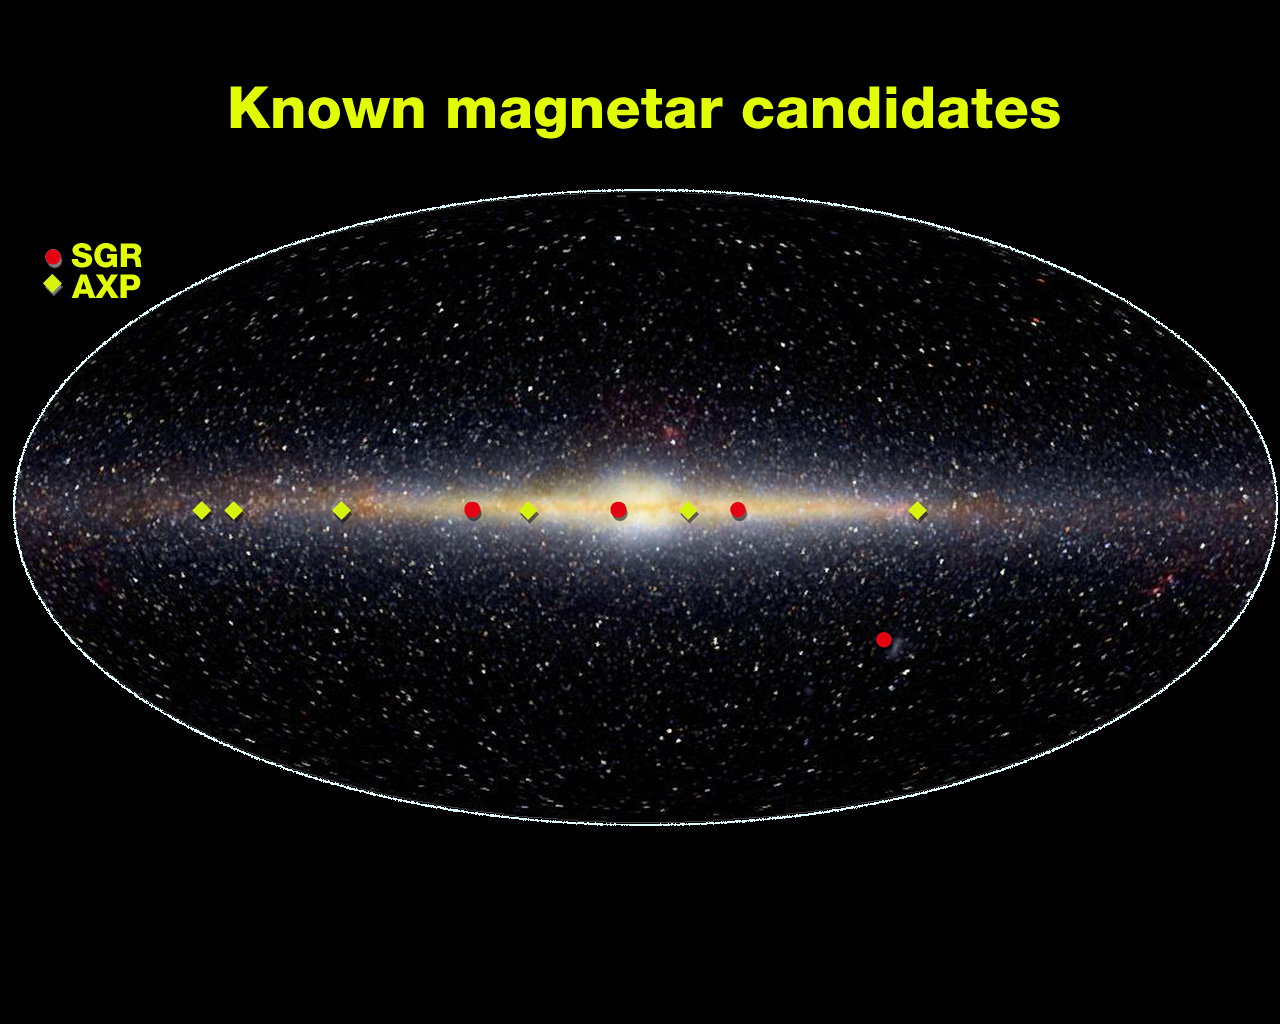
\includegraphics[width=0.6\textwidth]{./Sec_ET_ScienceCase/MagnetarLocations.jpg}
%\caption{The locations of known magnetar candidates (Soft Gamma-ray Repeaters and Anomalous X-ray Pulsars) in the Milky Way.  Credit: NASA/Marshall Space Flight Center}
%\end{center}
%%
%\end{figure}
Current models for SGRs~\cite{Pacheco98,Ioka01,Owen05} indicate that they will emit less than $10^{46} \,\mathrm{ergs}$ in GWs.  In the left panel of Fig.~\ref{fig:EnergyFreq_SGR} we show 90\%-confidence lower limits on the distances to which various GW detectors will be sensitive to GW bursts with this energy. We see that, in their most sensitive frequencies, the current generation of interferometers are just able to probe our own galaxy.  While advanced LIGO improves this reach substantially, it is really only with the ET that observations of GWs associated with extra-galactic SGR flares become possible.  Figure~\ref{fig:EnergyFreq_SGR} shows the complementary plot of 90\% energy upper limits obtainable by the various instruments for a galactic SGR (at a typical distance of $\sim 10$\,kpc).  Again, it is only with an instrument like ET that we are able to probe interesting energy regimes across the entire frequency spectrum one might reasonably expect for GW emission associated with SGR flares.



\FloatBarrier
\subsubsection{Probing Core-Collapse Supernova Physics}

Stellar collapse is one of the most energetic events in the Universe, releasing
$\sim 10^{53}\,\mathrm{erg}$ of gravitational energy in the compression of
a massive star's iron core to a NS. Most of this energy
($\sim99\%$) is emitted in neutrinos and only about
$10^{51}\,\mathrm{erg}$ go into energy of the core-collapse supernova
(CC-SN) explosion. CC-SNe (SN types II, Ib, Ic) are $\sim$10 times more
frequent than thermonuclear type-Ia SNe. A SN explosion pollutes the
interstellar medium with the nucleosynthetic products of stellar
evolution (CC-SNe are the Universe's primary source of oxygen) and
enriches the universe with rare heavy isotopes via the $r$-process. 
The perturbation caused by a SN in its vicinity can trigger the 
formation of stellar systems; CC-SNe are also the 
birth sites of NS and stellar-mass BH.

\paragraph{The Supernova Problem and GW observations}
The precise mechanism of explosion operating in CC-SNe is uncertain
\cite{bethe:90,janka:07,ott:09}. When the inner part of the collapsing
iron core reaches densities close to those in atomic nuclei, the
strong force leads to a stiffening of the nuclear EoS,
resulting in \emph{core bounce} of the inner core into the still
infalling outer core. A shock wave is formed that propagates outward
in mass and radius, but quickly loses energy due to the breakup of
heavy nuclei and neutrinos that carry away energy from the
postshock layer. The shock stalls, turns into an accretion shock and
must be \emph{revived} to drive a CC-SN explosion.  If this does not
happen, a BH will form on an accretion timescale of $\sim
2\,\mathrm{s}$. \emph{What is the mechanism of shock revival?}  This
is the fundamental question and primary unsolved problem of CC-SN
theory. Indications are strong that the CC-SN mechanism involves a
multitude of multi-dimensional processes, including rotation,
convection/turbulence, and various hydrodynamic instabilities of the
stalled shock and in the proto-NS. This opens up the possibility of
probing the supernova mechanism with GWs. 

GW, even more so than neutrinos, carry direct dynamical information
from the supernova engine deep inside a dying massive star, a region
generally inaccessible by the traditional means of observational
astronomy. GWs form a core-collapse event have the potential of
putting very strong constraints on the CC-SN mechanism
\cite{ott:09b,ott:09}.  With initial and certainly second-generation
interferometric GW detectors, this should be possible for an event in
the Milky Way ($D\sim 10$--$15\,\mathrm{kpc}$) and the Magellanic
Clouds~\cite{ott:09} ($D\sim 50$--$70\,\mathrm{kpc}$), but even
optimistic estimates of the CC-SN rate in this region do not predict
more than $\sim 1$--$2$~events per century. This number roughly doubles
if one includes the entire local group ($D\sim1\,\mathrm{Mpc}$). In
the region from $3$--$5\,\mathrm{Mpc}$ a number of starburst galaxies
increase the predicted and observed integrated SN rate to $\sim
0.5\,\mathrm{yr}^{-1}$. At $D\sim 10\,\mathrm{Mpc}$ it is
$\gtrsim 1\,\mathrm{yr}^{-1}$ \cite{ando:05}.
%
\begin{figure}
\centering
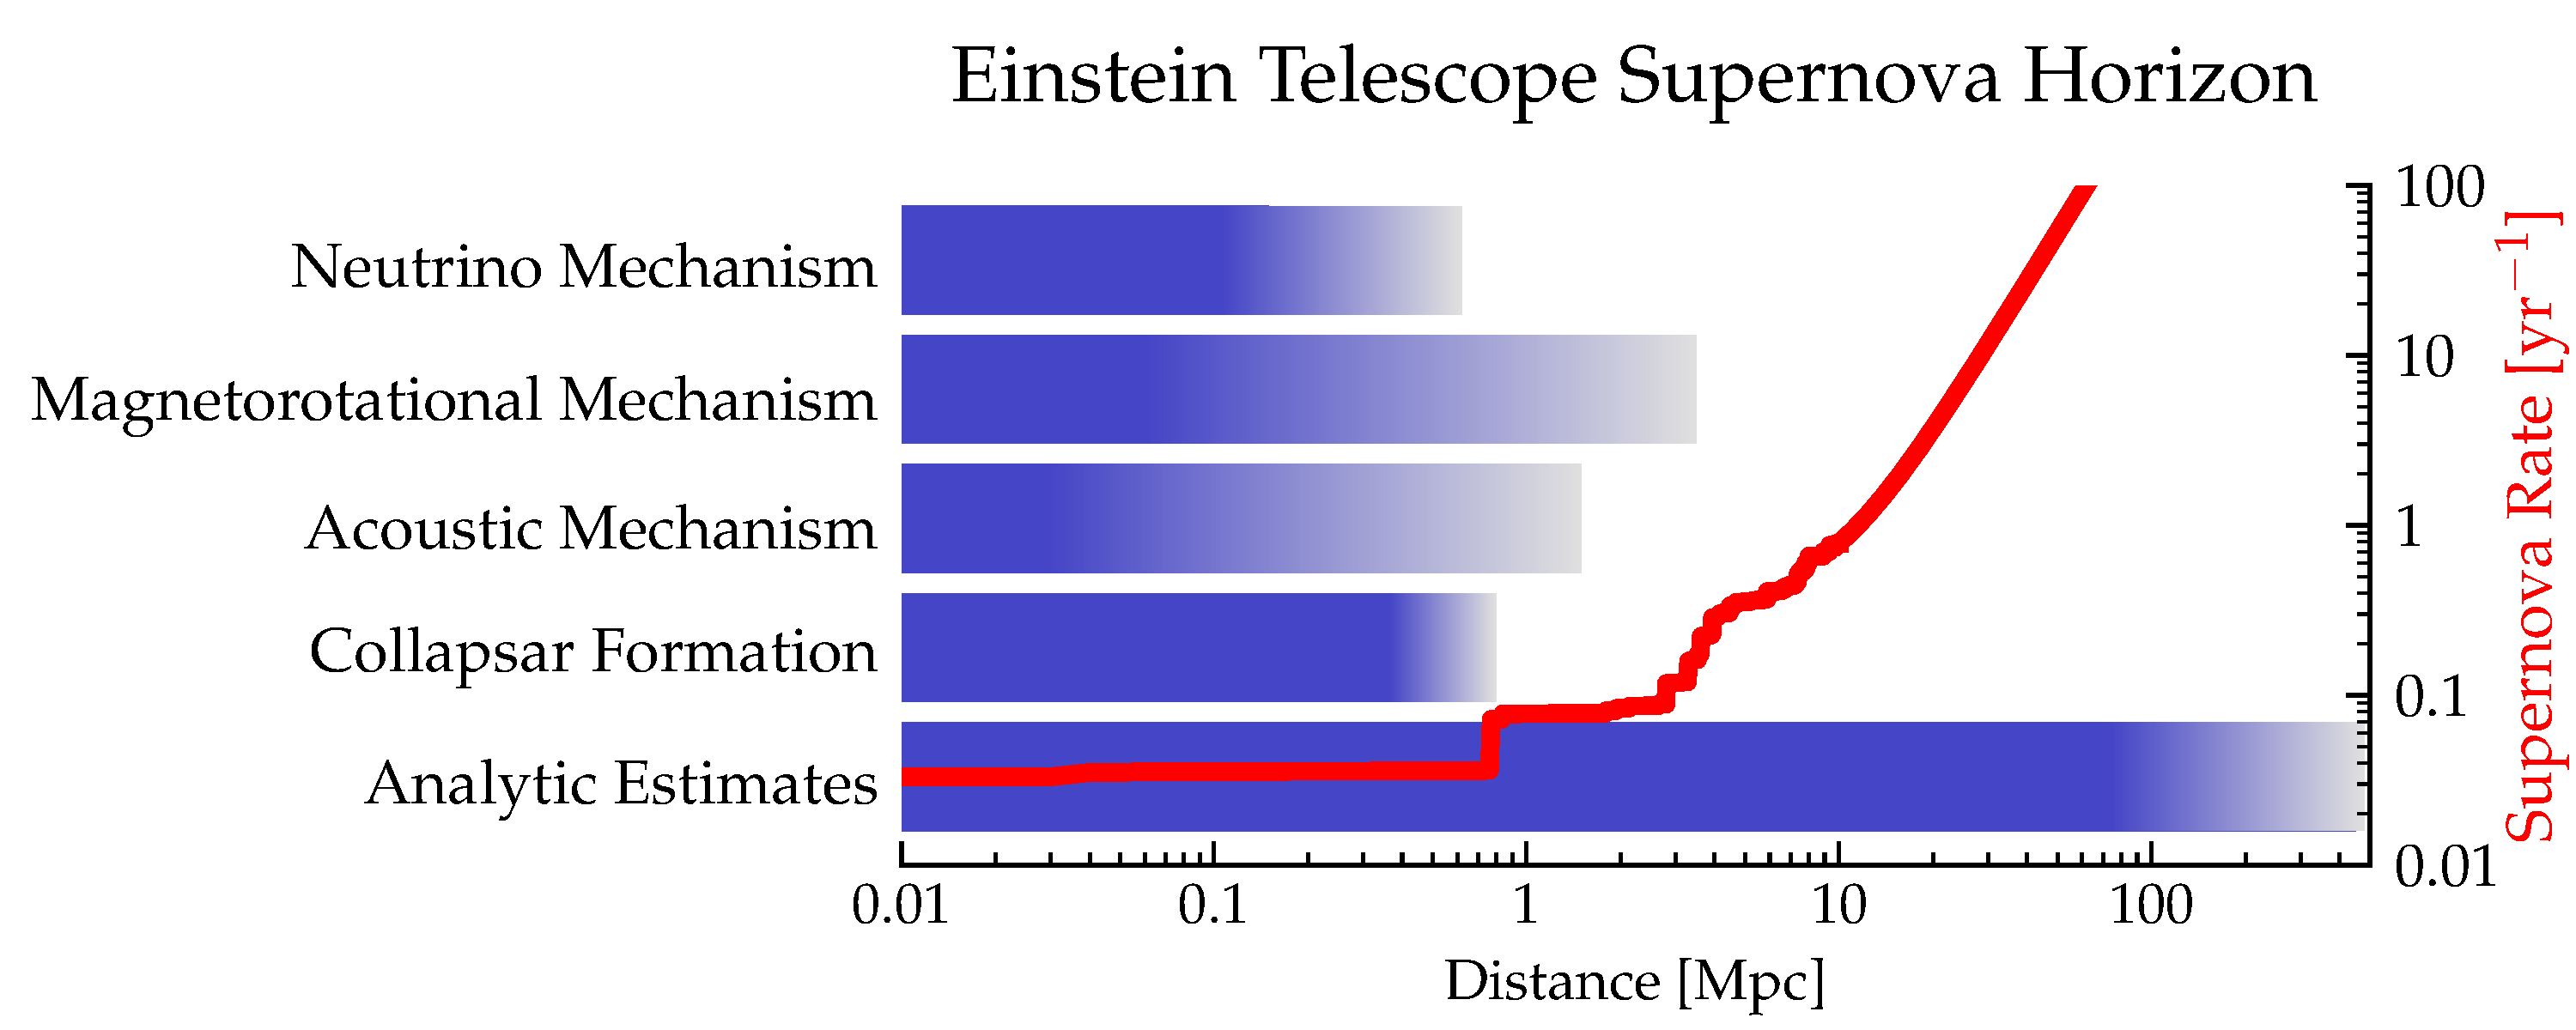
\includegraphics[width=0.85\columnwidth]{./Sec_ET_ScienceCase/ET_CCSN.pdf}
\caption{The plot displays ET's distance reach for different mechanisms
of supernovae as blue horizontal bars.  The plot also shows an estimate 
of the cumulative event rate (red curve) obtained
from the star formation rate computed over a catalogue of nearby galaxies
\cite{2005PhRvL..95f1103A}.\label{fig:supernova_rate}}
\end{figure}


\paragraph{Supernova Science with ET} 
The GW emission processes in a core collapse
event give rise to strains $h$ in the range $10^{-24}$--$10^{-22}$\,($D / 1\,
\mathrm{Mpc}$) and most of the emission takes place at frequencies of
$\sim 200$--$1000\,\mathrm{Hz}$, but the various explosion scenarios
exhibit unique spectral distributions and vary in total emitted
energies~\cite{ott:09,ott:09b}.  In addition, there is likely to be a
low-frequency GW-memory-type\footnote{The GW non-linear memory effect is a 
small, non-oscillatory contribution to the GW amplitude \cite{Blanchet:1992br,
Christodoulou:1991cr} The memory effect causes a permanent displacement 
of the test masses after the waves have passed.}
component with large $h$ up to
$10^{-22}\,(D / 1\,\mathrm{Mpc})$ at $0$--$20\,\mathrm{Hz}$.  ET as
currently envisioned is sufficiently sensitive to detect GWs
from various CC-SN scenarios out to $2$--$4\,\mathrm{Mpc}$. 

Core-collapse supernovae may lead to the emission of GWs
via a variety of multi-dimensional dynamical processes (see
e.g.\ \cite{ott:09} for a review) that are connected to the
prominent mechanism driving the explosion. Fig.~\ref{fig:supernova_rate} 
depicts reach estimates based on the GW burst analysis of simulated
ET noise with injected model waveforms using the X-Pipeline
\cite{sutton:10,kalmus:11}, assuming a single detector, optimal orientation,
one-hour on-source windows, and requiring 90\% detection confidence.

Model waveforms for GWs from neutrino-driven core-collapse
supernovae were drawn from \cite{ott:09,marek:09b,murphy:09,yakunin:10},
the model waveforms from \cite{scheidegger:10b,dimmelmeier:08} were used
for magnetorotational explosions, and the waveforms of \cite{ott:09}
were used to characterize explosions driven by the acoustic mechanism
proposed by \cite{burrows:06}. In addition, GW emission
from failing core-collapse supernovae that form BHs
(using the waveforms of \cite{ott:11a}) and analytic upper limits on the
GW signal in massive star collapse by \cite{fryer:02,piro:07}
are included.
The reach estimates are contrasted with the supernova rate in the
local universe obtained from \cite{ando:05} out to 10\,Mpc and assuming
a conservative rate of $10^{-4}$ core-collapse supernovae per Mpc$^3$
\cite{strigari:05} at greater distances.

ET may see multiple CC-SNe during its lifetime 
and would have the power to provide strong hints for a particular SN mechanism 
and/or smoking-gun evidence against another -- crucial astrophysics
information that is unlikely to be attainable in other ways.  At the time when 
ET is implemented, megaton-class neutrino detectors will be operating
and, having a range similar to ET, will be able to provide coincident
observations, narrowing down the time of the GW emission to $\sim
1\,\mathrm{ms}$. In addition, deep high-cadence optical transient
surveys will be in progress and targeting near-universe transients,
providing additional coincident data as well as additional astrophysical 
information, for instance on progenitor type/mass and explosion morphology/energy.

Constraining the CC-SN mechanism will mean
a breakthrough in our understanding of the large range of phenomena
associated with stellar collapse, CC-SNe, BH and NS formation, and
gamma-ray bursts (GRBs). However, the astrophysics and physics
information provided by GWs observed from a core collapse event with ET goes
beyond this. These GWs carry also information on the high-density nuclear EoS,
explosion asymmetries and pulsar kicks, the formation of a BH in a
failing CC-SN, and can help uncover rare events such as
the accretion-induced collapse of a white dwarf to a NS, or weak or failing
CC-SNe that have very weak or absent EM signatures.


%\FloatBarrier
%\subsubsection{Explaining neutron star spin frequencies in low-mass X-ray binaries}
%
%Observations of accreting NSs lead to perhaps the most
%important reason why, irrespective of the mechanism at work, at least
%some NSs might actually be emitting detectable gravitational
%waves.  This is the observation that even the fastest accreting
%NSs spin at rates much lower than the expected break-up
%frequency.  The current record is 716\,Hz \cite{Hessels:2006ze},
%while the theoretically expected upper limit is more than 1\,kHz. %% **cites**.
%Following a suggestion by Bildsten \cite{Bildsten:1998ey}, it is
%possible that this limit occurs because of the balance between the
%spin-up torque due to the accreting matter, and the spin-down torque
%due to GW emission.  A short calculation assuming a
%link between the observed X-ray luminosity with the accretion rate,
%and taking the mountain scenario for the emission mechanism leads to
%the following estimate of the GW amplitude:
%\begin{equation}
  %\label{eq:6_again}
  %h_0 = 3 \times 10^{-27}F_{-8}^{1/2}\left(\frac{R}{\rm 10
        %km}\right)^{3/4}\left(\frac{1.4 M_\odot}{M}\right)^{1/4}
  %\left(\frac{{\rm 1~kHz}}{\nu_s}\right)^{1/2}.
%\end{equation}
%This is seen to be dependent on frequency: $h_0 \propto \nu_s^{-1/2}$.
%%
%\begin{figure}[htb]
%\centering
%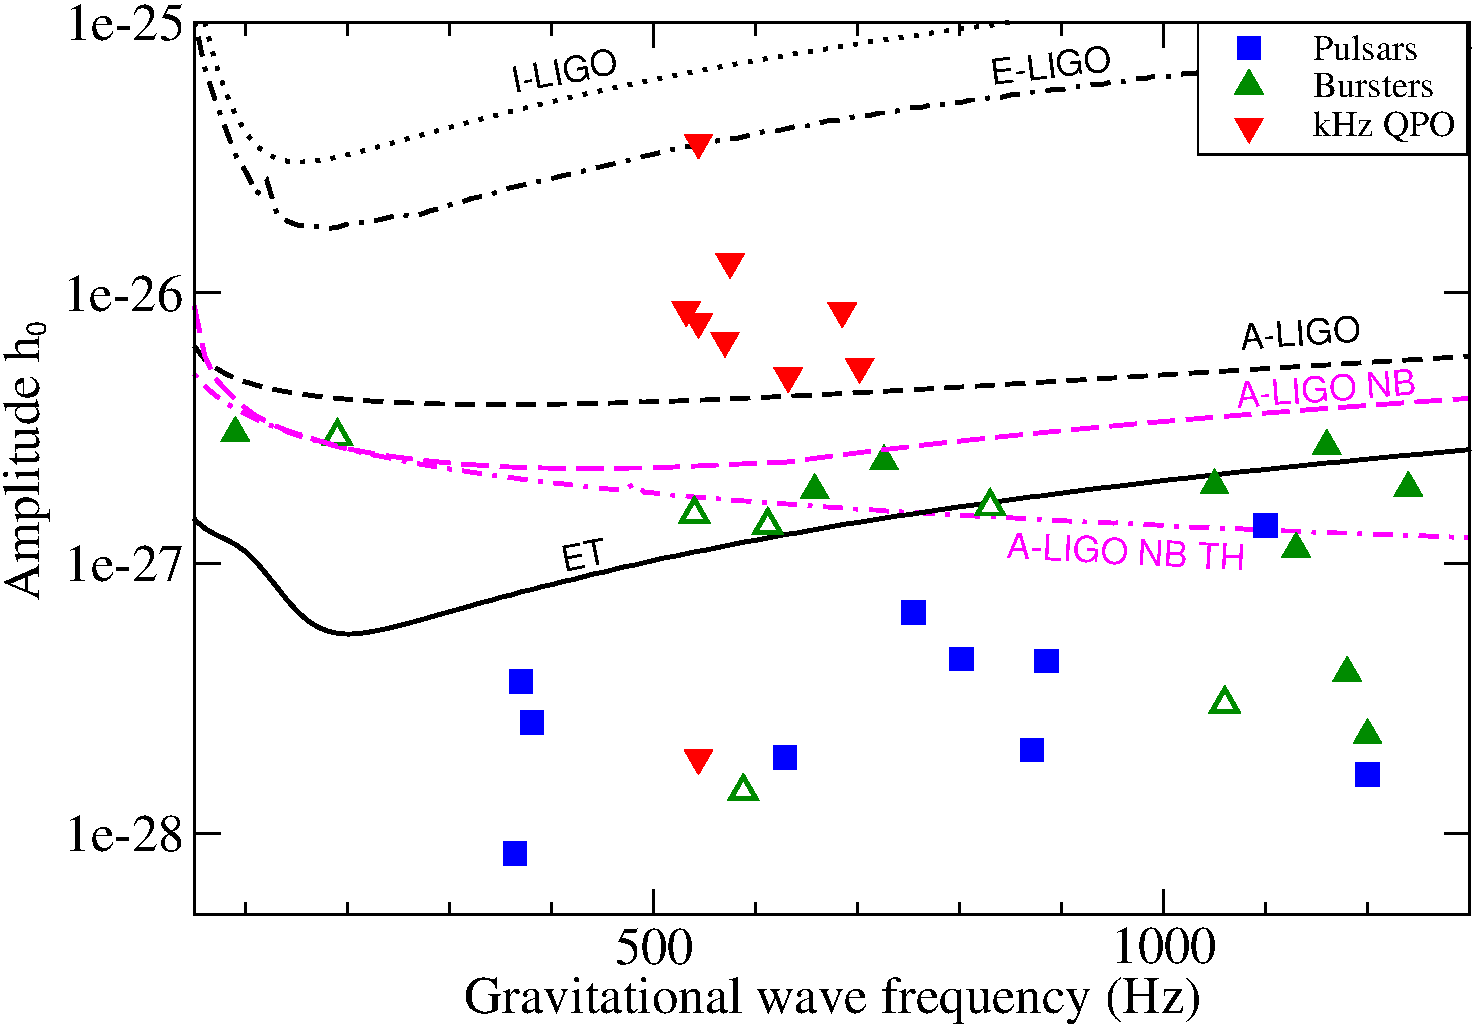
\includegraphics[angle=0,width=0.65\textwidth]{./Sec_ET_ScienceCase/CW_lmxb}
%\caption{Sensitivity and the spin-balance limit for the accreting
  %neutron stars.}
%\label{fig-CW-spin}
%\end{figure}

%% Spin frequency measurement plays an important role in what follows
%% and, as we shall see, can \cite{Watts2008}
%\begin{figure}
%\centering
%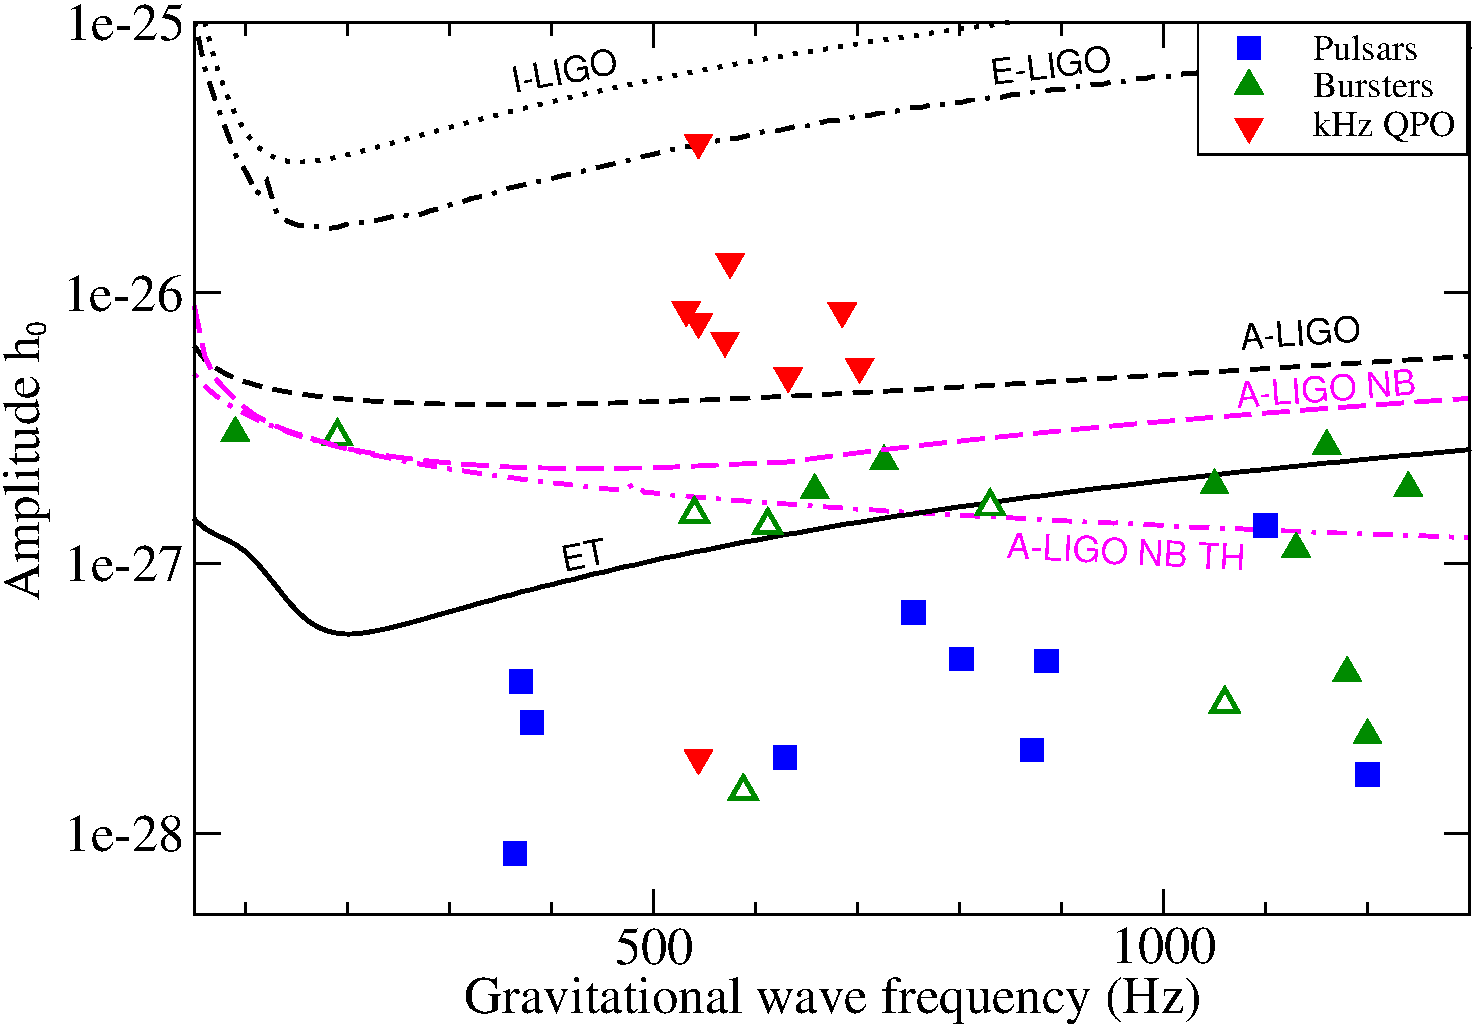
\includegraphics[angle=0,width=0.5\columnwidth]{./Sec_ET_ScienceCase/CW_lmxb.pdf}
%\caption{Sensitivity and the spin-balance limit for the accreting
%  neutron stars.}
%\label{fig-CW-spin}
%\end{figure}
%\subsubsection{Radio pulsars and magnetars as sources of GW and their structure}
%\dots
%\subsubsection{Are intermediate-mass black holes behind ULX sources?}
%\dots

\clearpage
\FloatBarrier
\subsection{Cosmology and Cosmography}
ET can observe coalescences of stellar mass BBHs all the way up 
to the edge of the Universe at redshifts $z>15,$ BNS
can be detected from $z\sim 1$-2 when the star formation 
rate in the Universe was at its peak and IMBBHs
are accessible at a redshift range of $z\sim 2$-10 depending on the
total mass and mass ratio of the binary (see Fig.\,\ref{fig:ET_range}).
A large population of such events provides markers distributed
throughout the Universe with accurately known luminosity distance 
and redshift (if the host galaxy could be identified). 
ET's three interferometers will also be sensitive to stochastic 
background radiation from primordial process and astronomical 
populations distributed throughout the Universe. Here we will
discuss how ET can be a very powerful tool for cosmography
and the early Universe.

\FloatBarrier
\subsubsection{Cosmography with a population of standard sirens}

% \ledby{Sathya}

The goal of modern cosmology is to measure the geometrical and
dynamical properties of the Universe by projecting the observed
parameters onto a cosmological model. The Universe has a lot
of structure on small scales, but on a scale of about
100\,Mpc %%\footnote{$1 {\rm Mpc} \simeq 3.09 \times 10^{16}\rm m.$}
the distribution of both baryonic (inferred from the
electromagnetic radiation it emits) and dark matter (DM)
(inferred from large scale streaming motion of galaxies)
components is quite smooth. It is, therefore, quite
natural to assume that the Universe is homogeneous and
isotropic while describing its large-scale properties.
In such a model, the scale factor $a(t)$, which essentially
gives the proper distance between comoving coordinates, and
curvature of spatial sections $k$, are the only quantities
that are needed to fully characterize the properties of
the Universe. The metric of a smooth homogeneous
and isotropic spacetime is
\begin{equation*}  % changed to version with "*" to remove the equation number (PW)
ds^2 = -dt^2 + a^2(t) \frac{d\sigma^2}{1 - k\sigma^2}
+ \sigma^2 \left (d\theta^2 + \sin^2\theta\, d\varphi^2 \right ),
%\nonumber % commented out (PW) - caused pdfTeX warning "destination with the same identifier..."
\end{equation*}
where $t$ is the cosmic time-coordinate, $(\sigma,\,\theta,\,
\varphi)$ are the comoving spatial coordinates, and $k$ is
a parameter describing the curvature of the $t=\rm const.$ 
spatial slices: $k=0,\,\pm 1$ for flat, positively
and negatively curved slices, respectively.
The evolution of $a(t),$ of course, depends on the parameter
$k$ as well as the ``matter" content of the Universe. The latter
could consist of radiation, baryons, DM, DE,
and any other possible contributions to the energy-momentum
tensor.

The Friedman equation, which is one of two Einstein
equations describing the dynamics of an isotropic and homogeneous
Universe, relates the cosmic scale factor $a(t)$ to the energy
content of the Universe through
\begin{equation}
H(t) = H_0 \left [ \hat\Omega_{\rm M}(t) - \frac{k}{H_0^2a^2} +
\hat\Omega_\Lambda(t)  \right ]^{1/2},
\label{eq:friedman_equation}
\end{equation}
where $H(t)\equiv \dot a(t)/a(t)$ is the Hubble parameter
($H_0=H(t_P)$ being its value at the present epoch $t_P$),
$\hat\Omega_{\rm M}(t)$ and $\hat\Omega_\Lambda(t)$ are the (dimensionless)
energy densities of the DM and DE, respectively.
The above equation has to be supplemented with the
EoS of DM, assumed to be pressure-less
fluid $p=0$ [$\hat\Omega_{\rm M}(t)=\Omega_M(1+z)^3,$
$\Omega_{\rm M}=\hat\Omega_{\rm M}(t_P)$]
and of DE, assumed to be of the form
$p = w\rho_{\Lambda}$ [$\hat\Omega_\Lambda(t)=\Omega_\Lambda(1+z)^{3(1+w)},$
where $\Omega_\Lambda=\Omega_\Lambda(t_P)$],
with $w=-1$ corresponding to a cosmological constant.
The goal of cosmography is to measure $(H_0,\,
\Omega_{\rm M},\, \Omega_\Lambda,\, w,\, k,\, \ldots),$
which essentially determine the large-scale geometry and
dynamics of the Universe.  In the rest of this section
we shall assume that the spatial slices are
flat (i.e.\  $k=0$).


\paragraph{Cosmic distance ladder} \label{cosmo_parameters}
Astronomers use ``standard candles'' to measure the geometry of
the Universe and the various cosmological parameters. A standard
candle is a source whose intrinsic luminosity $L$ can be inferred
from the observed properties (such as the spectral content,
time-variability of the flux of radiation, etc.). Since the
observations also measure the apparent luminosity $F$, one
can deduce the luminosity distance $D_{\rm L}$ to a standard
candle from $D_{\rm L}=\sqrt{L/(4\pi F)}$.
In addition, if the redshift $z$ to the source is known then
by observing a population of such sources it will be possible to
measure the various cosmological parameters since the luminosity
distance is related, when $k=0,$ to the redshift via Eq.\,(\ref{DLgeneral}).
%\begin{equation}
%D_{\rm L} = \frac{c (1+z)}{H_0} \int_0^z \frac{dz'}{\left [
%\Omega_{\rm M} (1+z')^3 + \Omega_\Lambda (1+z')^{3(1+w)} \right ]^{1/2}}.
%\label{eq:cosmology}
%\end{equation}
There is no unique standard candle in astronomy that works on all
distance scales. An astronomer, therefore, builds the distance scale
by using several steps, each of which works over a limited range of
the distance. For instance, the method of parallax can
determine distances to a few kpc,
Cepheid variables up to $10$\,Mpc, the
Tully-Fisher relation works for several tens of Mpc, the $D_n$-$\sigma$
relation up to hundreds of Mpc and Type Ia supernovae up to redshifts
of a few. This way of building the distance scale
has been referred to as the \emph{cosmic distance ladder}. For
cosmography, a proper calibration of the distance to high
redshift galaxies
is based on the mutual agreement between different rungs of this
ladder. It is critical that each of the rungs is calibrated
with as little an error as possible.


As discussed in Box \ref{box:lumdistcbc}, gravitational waves 
from inspiralling compact binaries are ideal standard candles.
Their dynamics is completely described by Einstein's equations
and have been computed in the post-Newtonian theory to a very
high order. They are free from complex astrophysical phenomena
which normally poses difficulties in treating most sources as
standard candles. Moreover, gravitational waves are not subject
to attenuation of various kinds that causes EM radiation to be
contaminated when travelling over cosmological distances. 
Gravitational astronomy is, therefore, able to supplement 
cosmological studies and could provide very valuable information
both about the sources as well as the geometry and structure of
the Universe.

For sufficiently low-redshift sources $(z\ll 1)$, the relationship 
between the luminosity distance of a source and its redshift is 
the Hubble law $D_{\rm L}=c z/H_0,$  where $v=c\,z$ is the cosmological 
recession velocity of the source. Therefore, one can measure the Hubble 
constant with an accurate measurement of the luminosity distance to a 
soure and its redshift.  With only 50 sources up to a redshift 
of $z = 0.5$, ET would determine $H_0 $ with an accuracy of 0.55\%
\cite{Sathyaprakash2009}.

\begin{wrapfigure}{r}{0.5\textwidth}
%\begin{figure}[tbh]
%\centering
%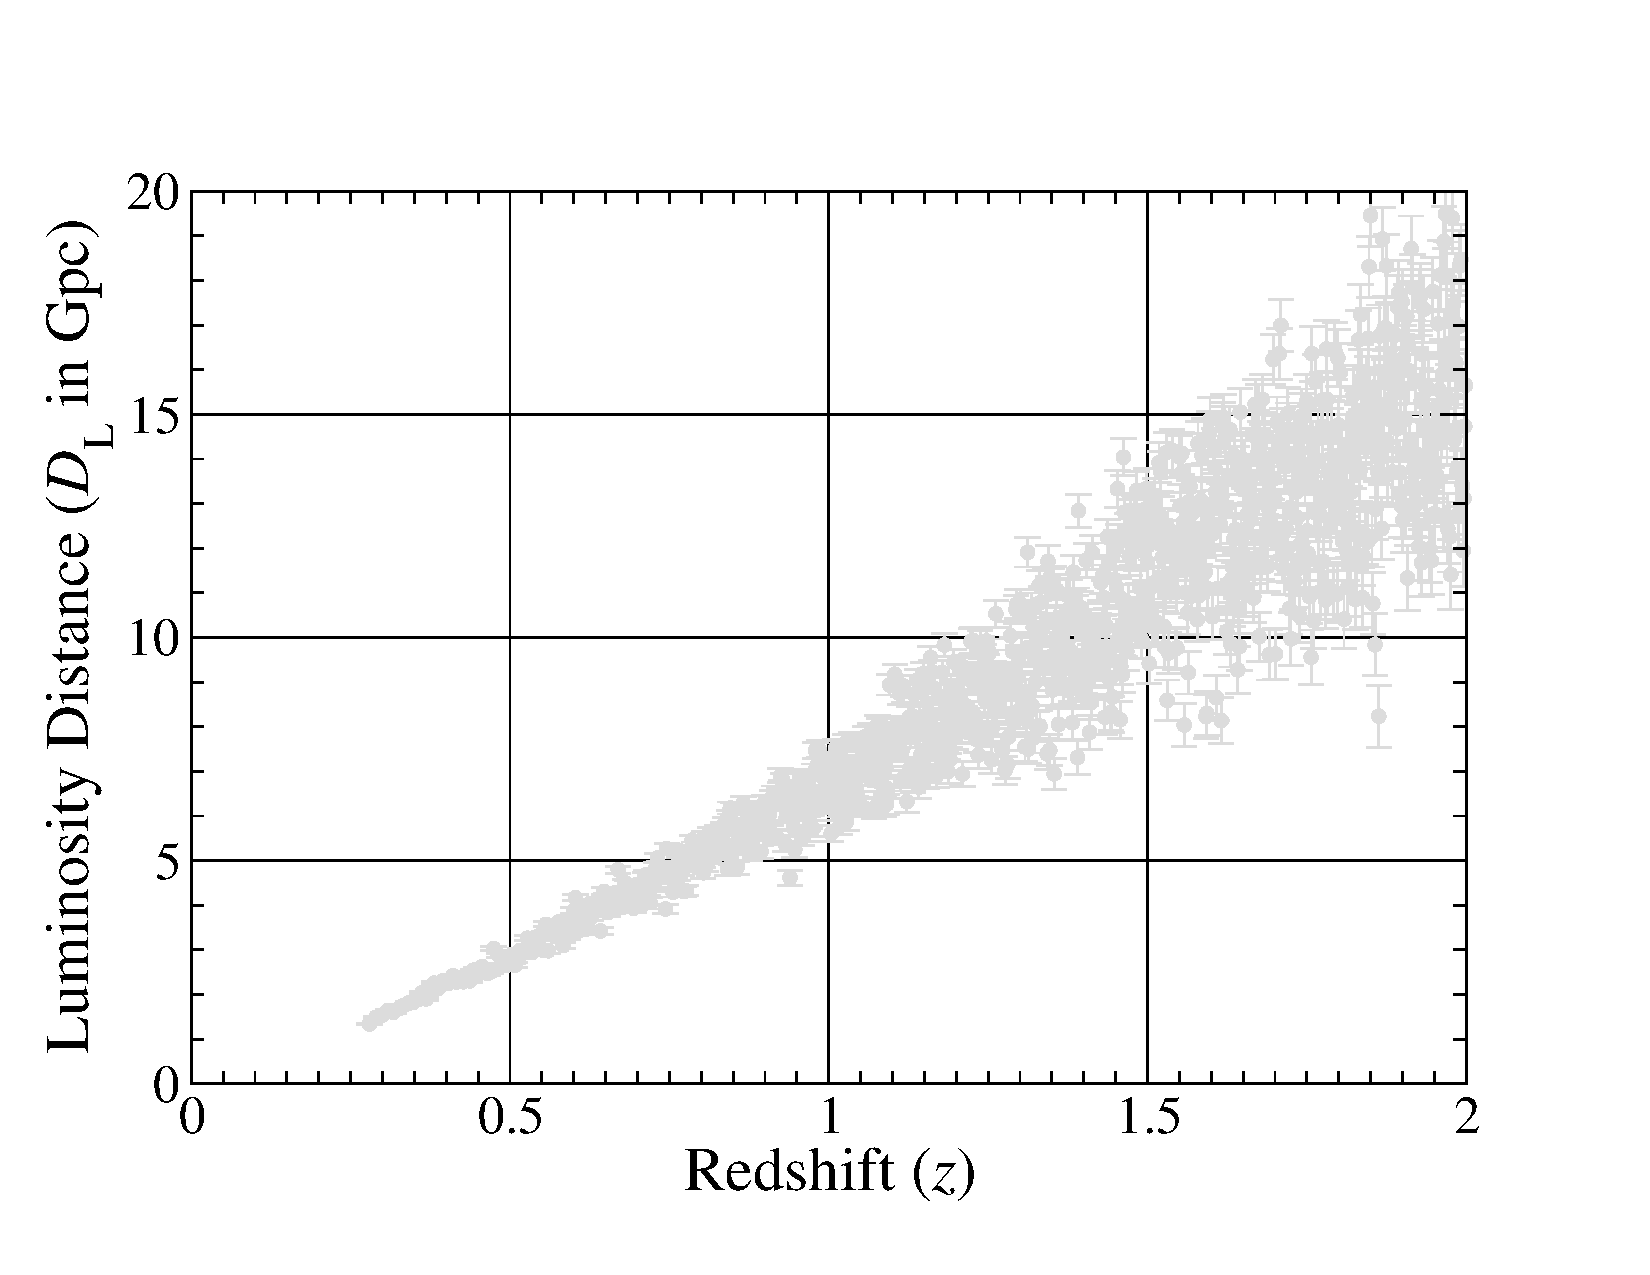
\includegraphics[width=0.45\textwidth]{./Sec_ET_ScienceCase/realization.pdf}
\vskip-0.5cm
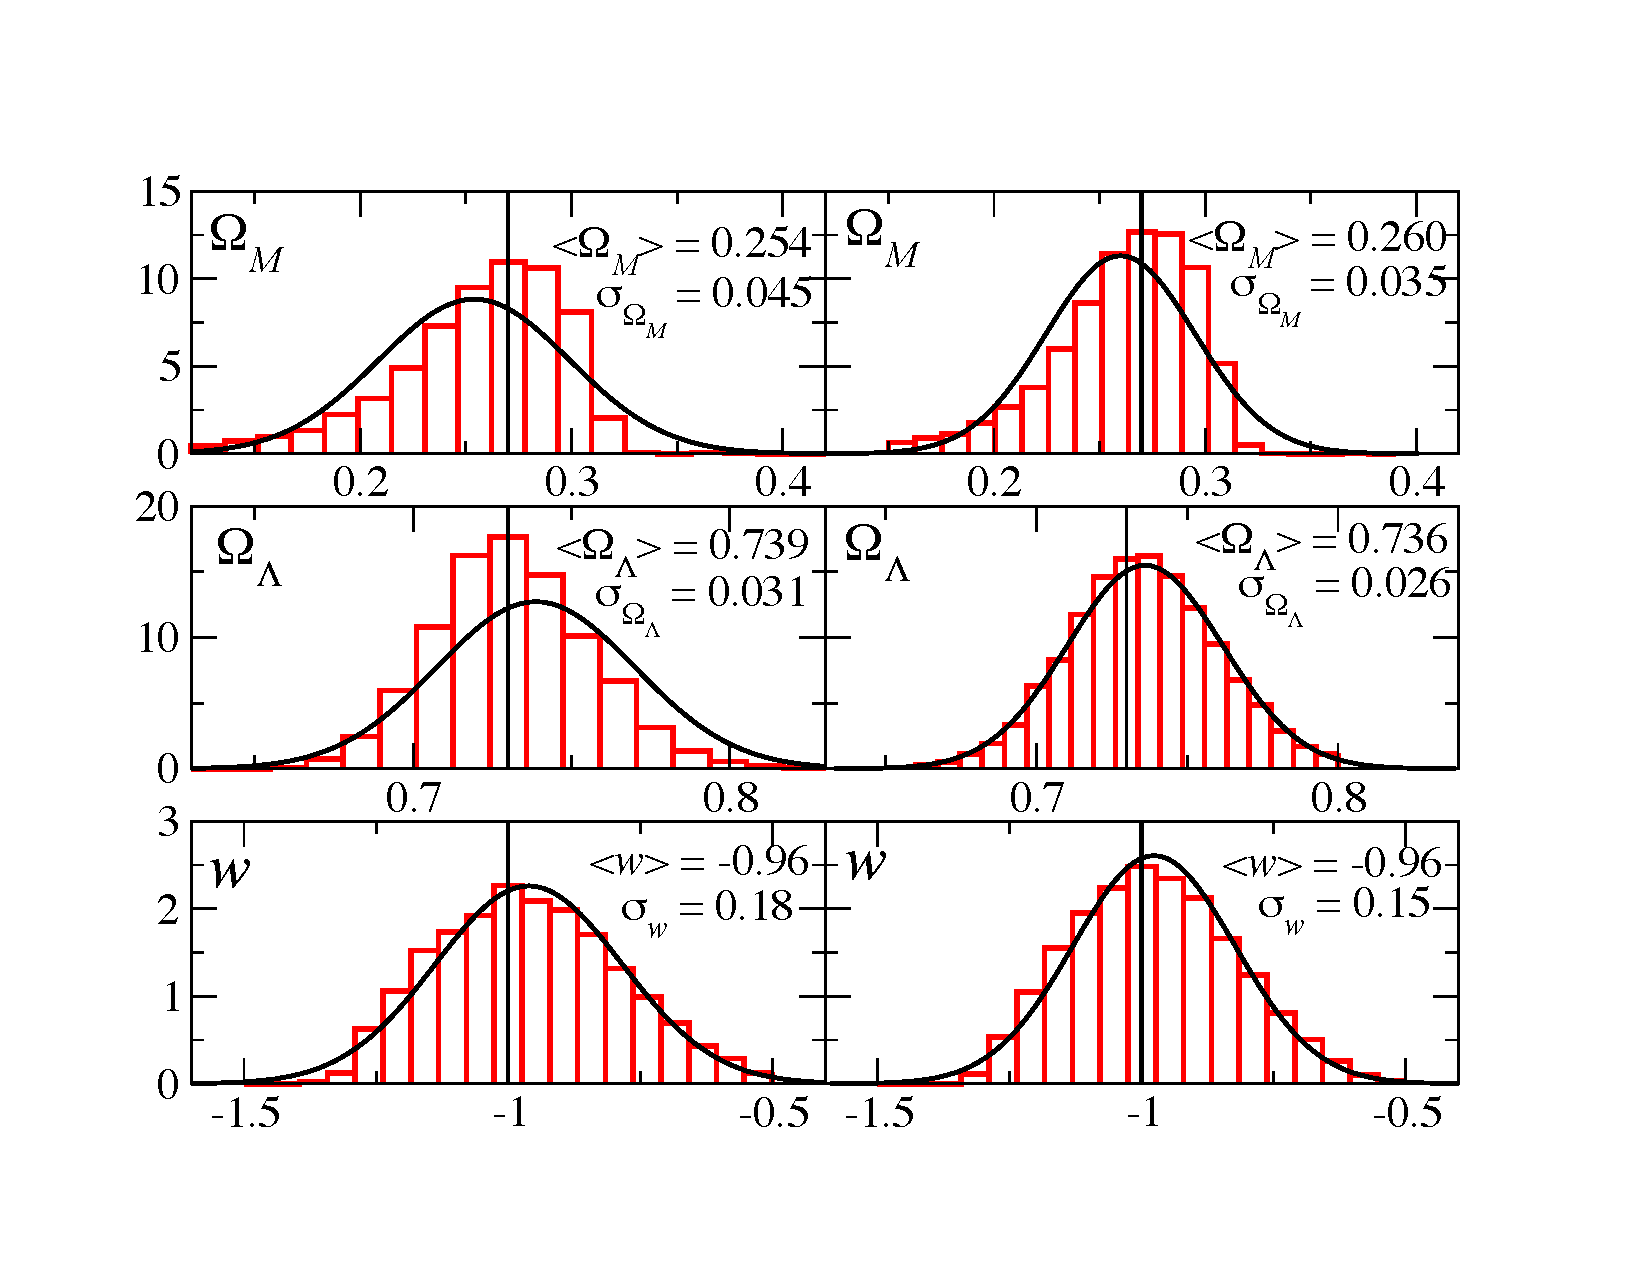
\includegraphics[width=0.5\textwidth]{./Sec_ET_ScienceCase/3params_combined.pdf}
\caption{
%The plot on the left shows one realization of a
%catalogue of binary neutron star (BNS) events that might
%be observed by ET. 
The distribution of errors in $\Omega_{\rm M},$
$\Omega_{\Lambda}$ and $w$ obtained by fitting 5,190
realizations of a catalogue of BNS merger events to a
cosmological model of the type given in
Eq.\,(\ref{DLgeneral}), with three free parameters.
The fractional 1-$\sigma$ width of the distributions
$\sigma_{\Omega_{\rm M}}/\Omega_{\rm M}$,
$\sigma_{\Omega_{\Lambda}}/\Omega_{\Lambda}$, and
$\sigma_w/|w|,$ are 18\%, 4.2\% and 18\%
(with weak lensing errors in $D_{\rm L}$, left panels)
and 14\%, 3.5\% and 15\% (if weak lensing
errors can be corrected, right panels).}
\vskip-0.5cm
\label{fig:fits}
%\end{figure}
\end{wrapfigure}
\paragraph{Cosmology from a population of compact binaries} 
As discussed in Section \ref{sec:binaries}, the expected rate 
of mergers within the horizon of ET is $\sim {\rm several}\times 
10^5\,\rm yr^{-1}$ for BNS and NSBH systems.
Such a large population of events with
luminosity distances measured to good accuracy
would be very useful for measuring cosmological parameters.
If, as suspected, BNS and NSBH systems are progenitors of short-hard
gamma-ray bursts (GRBs) \cite{2006ApJ...640..849N}, then it might be possible
to make a coincident detection of a significant subset of
the events in GW and EM windows and obtain
both the luminosity distance and redshift of the source.

Since GRBs are believed to be beamed with beaming angles
of order $40^\circ$, we assume
that only a small fraction ($\sim 10^{-3}$) of binary coalescence
events will have GRB or other EM afterglows that will help us
to locate the source on the sky and measure its
redshift $z$. Eventually, we will be limited by the
number of short-hard GRBs observed by detectors that might
be operating at the time. As a conservative estimate, we
assume that about $1,000$ BNS and NSBH mergers will have
EM counterparts over a three-year period. For definiteness we
consider only BNS mergers and take
these to have component masses of $(1.4,1.4) M_\odot$.

How well would we measure cosmological parameters with a
catalogue of such sources? The detailed procedure followed to
evaluate this is given in Box \ref{box:cosmo params}.

The distributions ${\cal P}$ of the cosmological parameters obtained
from a three year catalogue of binary neutron star inspirals is shown 
in Fig.~\ref{fig:fits} assuming $(\Omega_{\rm M},\, \Omega_\Lambda,\, w)$
are all unknown, in the left panel of 
Fig.\,\ref{fig:fits2} assuming $\Omega_\Lambda$ is unknown (say from
other cosmological probes) and that $(\Omega_{\rm M},\, w)$ are unknown
and in the right panel of 
Fig.\,\ref{fig:fits2} assuming that $w$ is the only unknown parameter.

%
\longetbox{r}{box:cosmo params}
{ET for cosmography}
{
To evaluate how well  ET can measure various cosmological 
parameters we simulated 5,190 realizations
of a catalogue of BNS sources that ET is expected to detect. 
Each catalogue contained 1,000 BNS coalescences
with known redshift and sky location. The luminosity
distance to the sources is subject to statistical errors 
from GW observation and weak lensing that the waves suffer
when propogating through the clumpy dark matter distribution
in the inter-galactic medium.
\\[5pt]
We assumed that the sources were in the redshift range 
$0\le z \le 3.5$, distributed uniformly (i.e.\  with constant 
comoving number density) throughout this redshift range. The 
luminosity distance to the source was computed by assuming an 
FLRW cosmological model with $H_0=70\,{\rm km\,s^{-1}\,Mpc^{-1}}$,
$\Omega_{\rm M}=0.27$, $\Omega_\Lambda=0.73$, and $w=-1$, 
but the \emph{measured} distance was drawn from a Gaussian 
distribution whose width, $\sigma_{D_{\rm L}}$, was determined 
by the quadrature sum of the errors due to weak lensing
and GW observation. The weak lensing error in $D_{\rm L}$
was assumed to be 5\% at $z=1$ and linearly extrapolated to 
other redshifts.  
\\[5pt]
The GW observational error was estimated from the covariance matrix 
$C_{km}$ of the five-dimensional parameter space of the unknown signal
parameters $p_k = (M,\nu,t_0,\Phi_0, D_{\rm L})$:
\begin{equation}
C_{km} = \Lambda_{km}^{-1},\quad \Lambda_{km} = \left < h_k,\, h_m \right >,
\quad h_k = \frac{\partial h}{\partial p_k}.
\end{equation}
Here the angular brackets denote the scalar product, which,
for any two functions $a(t)$ and $b(t)$, is defined as
\begin{equation}
\left < a,\, b \right > = 4 \Re \int_0^\infty \frac{{\rm d}f}{S_h(f)}
A(f)\,B^*(f)
\end{equation}
where $A(f)$ and $B(f)$ are the Fourier transforms of the
functions $a(t)$ and $b(t)$, respectively, and $S_h(f)$ is the ET
noise power spectral density.  
\\[5pt]
Since GRBs are expected to be strongly beamed, we assumed the 
angles $(\iota,\psi)$ defining the unit normal to the plane 
of the inspiral to be known. This assumption is well-justified 
because even if the opening angle of a GRB beam is as large as 
$40^\circ$, the unit normal to the plane of the inspiral would still 
be confined to only 3\% of the area of a unit sphere. Averaging 
errors over $(\iota,\psi)$ with the constraint $\iota < 20^\circ$
would then be little different from taking $\iota = 0^\circ$. 
We did, however, average the errors over the sky position angles 
$(\theta,\phi)$.  
\\[5pt]
We fitted each realization of the source 
catalogue to the cosmological model given in Eq.\,(\ref{DLgeneral}), 
using the Levenberg-Marquardt algorithm \cite{Levenberg:1944,Marquardt:1963}, 
in order to find a set of best fit parameters.  
Assuming that $H_0$ is known accurately (see discussion in the text as to
how ET will measure $H_0$ to better than 1\% from low redshift sources), 
the algorithm gave the best fit parameters in $(\Omega_{\rm M},\,
\Omega_\Lambda,\, w)$ for each of the 5,190 realizations.
The distributions ${\cal P}$ of the parameters obtained
are shown in Fig.~\ref{fig:fits}, where the
vertical line is at the true value of the relevant parameter
(see text for a discussion of the results). 
}

The relative
1-$\sigma$ errors in $\Omega_{\Lambda},$  $\Omega_{\rm M}$ and $w,$
are 4.2\%, 18\% and 18\% (with weak lensing, left panels) and
3.5\%, 14\% and 15\% (with weak lensing errors corrected, right panels).
Although ${\cal P}(w)$ is quite symmetric,
${\cal P}(\Omega_{\rm M})$ and ${\cal P}(\Omega_\Lambda)$
are both skewed and their mean values are slightly off
the true values. However, the medians are mostly coincident with
the true values.

In addition to $H_0$ if $\Omega_{\Lambda}$ is also known (or, equivalently,
if $\Omega_{\rm M}+\Omega_{\Lambda}=1$), then one can estimate the
pair $(\Omega_{\rm M},\,w)$ more accurately, with the distributions
as shown in Fig.~\ref{fig:fits} with greatly reduced skewness
and 1-$\sigma$ errors in $\Omega_{\rm M}$ and $w,$ of 9.4\% and 7.6\%
(with weak lensing) and 8.1\% and 6.6\% (with lensing errors corrected).
Finally, if $w$ is the only parameter unknown, it can be measured to
an even greater accuracy as shown in Fig.~\ref{fig:fits2} with
1-$\sigma$ errors of 1.4\% (with weak lensing) and 1.0\% (with lensing
errors corrected).


\begin{figure*}[t]
\centering
 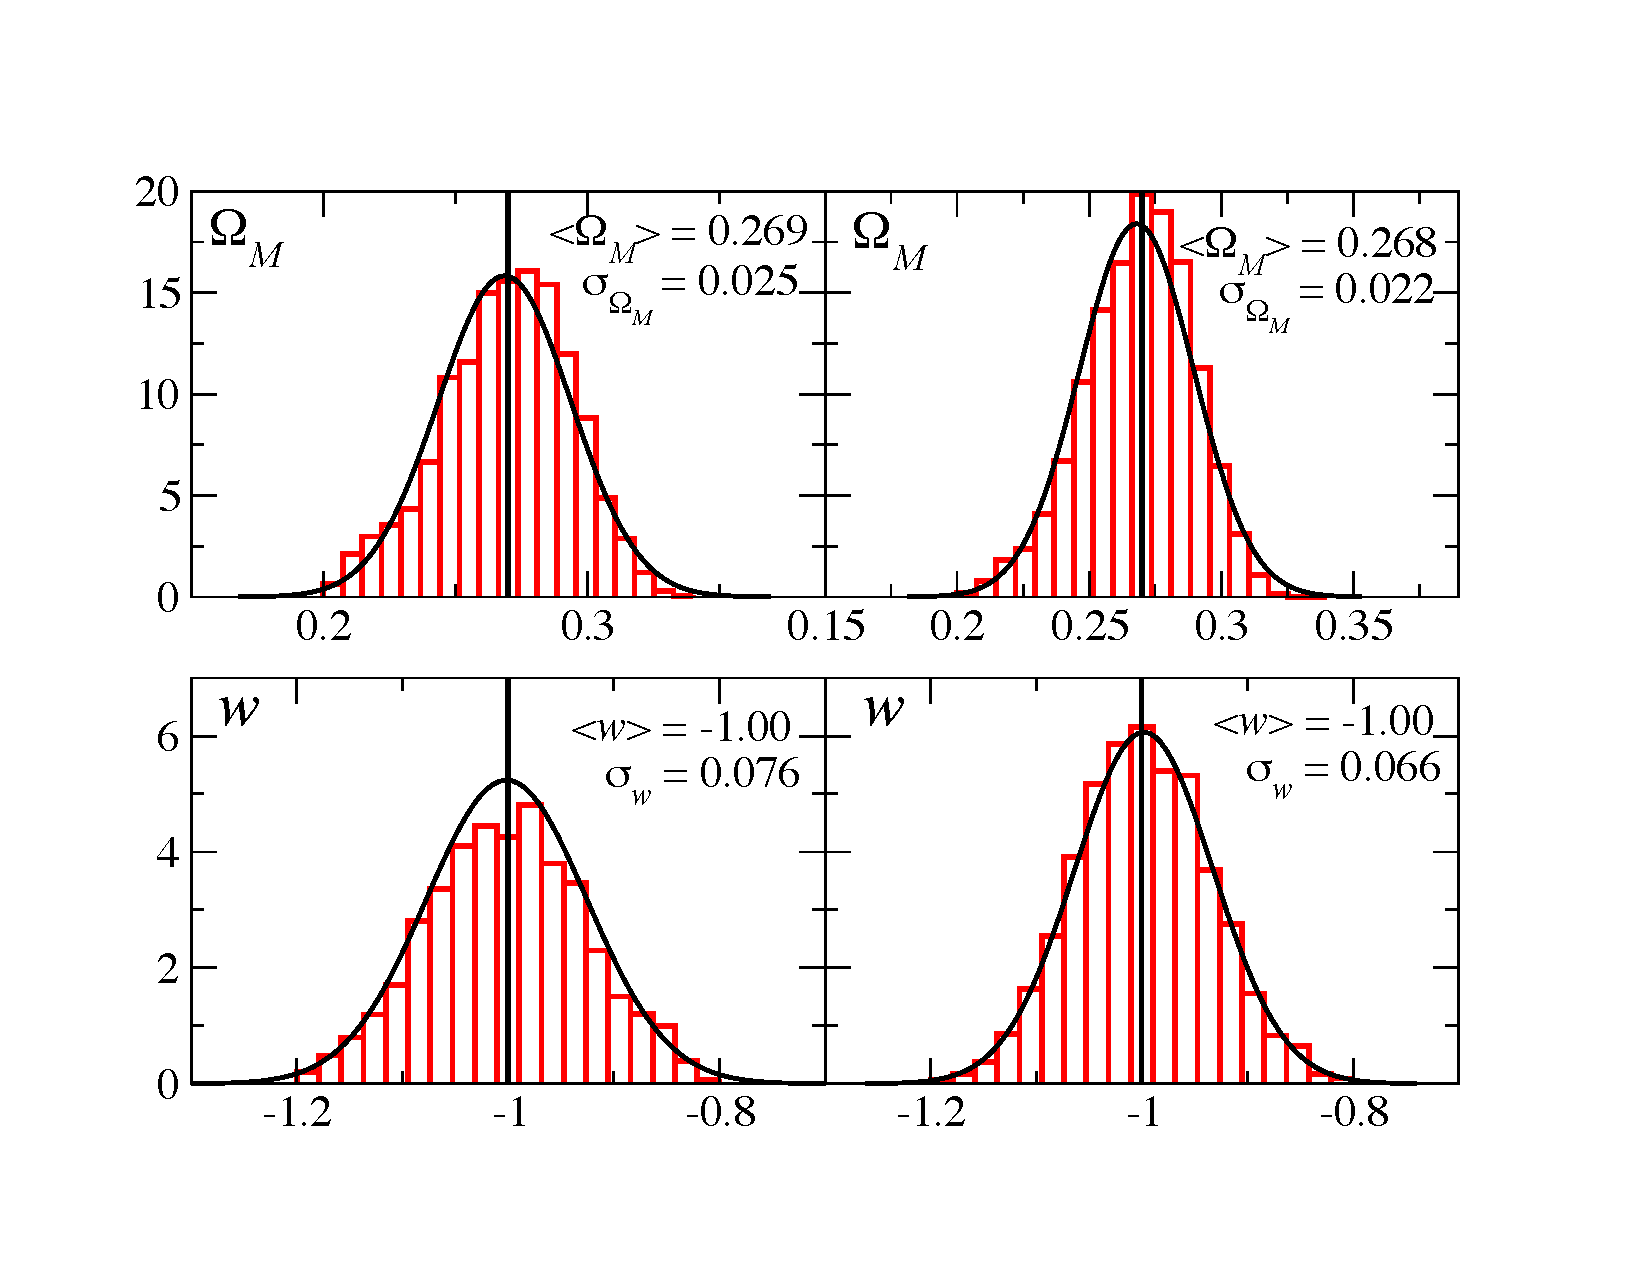
\includegraphics[width=0.45\textwidth]{./Sec_ET_ScienceCase/2params_combined.pdf}
 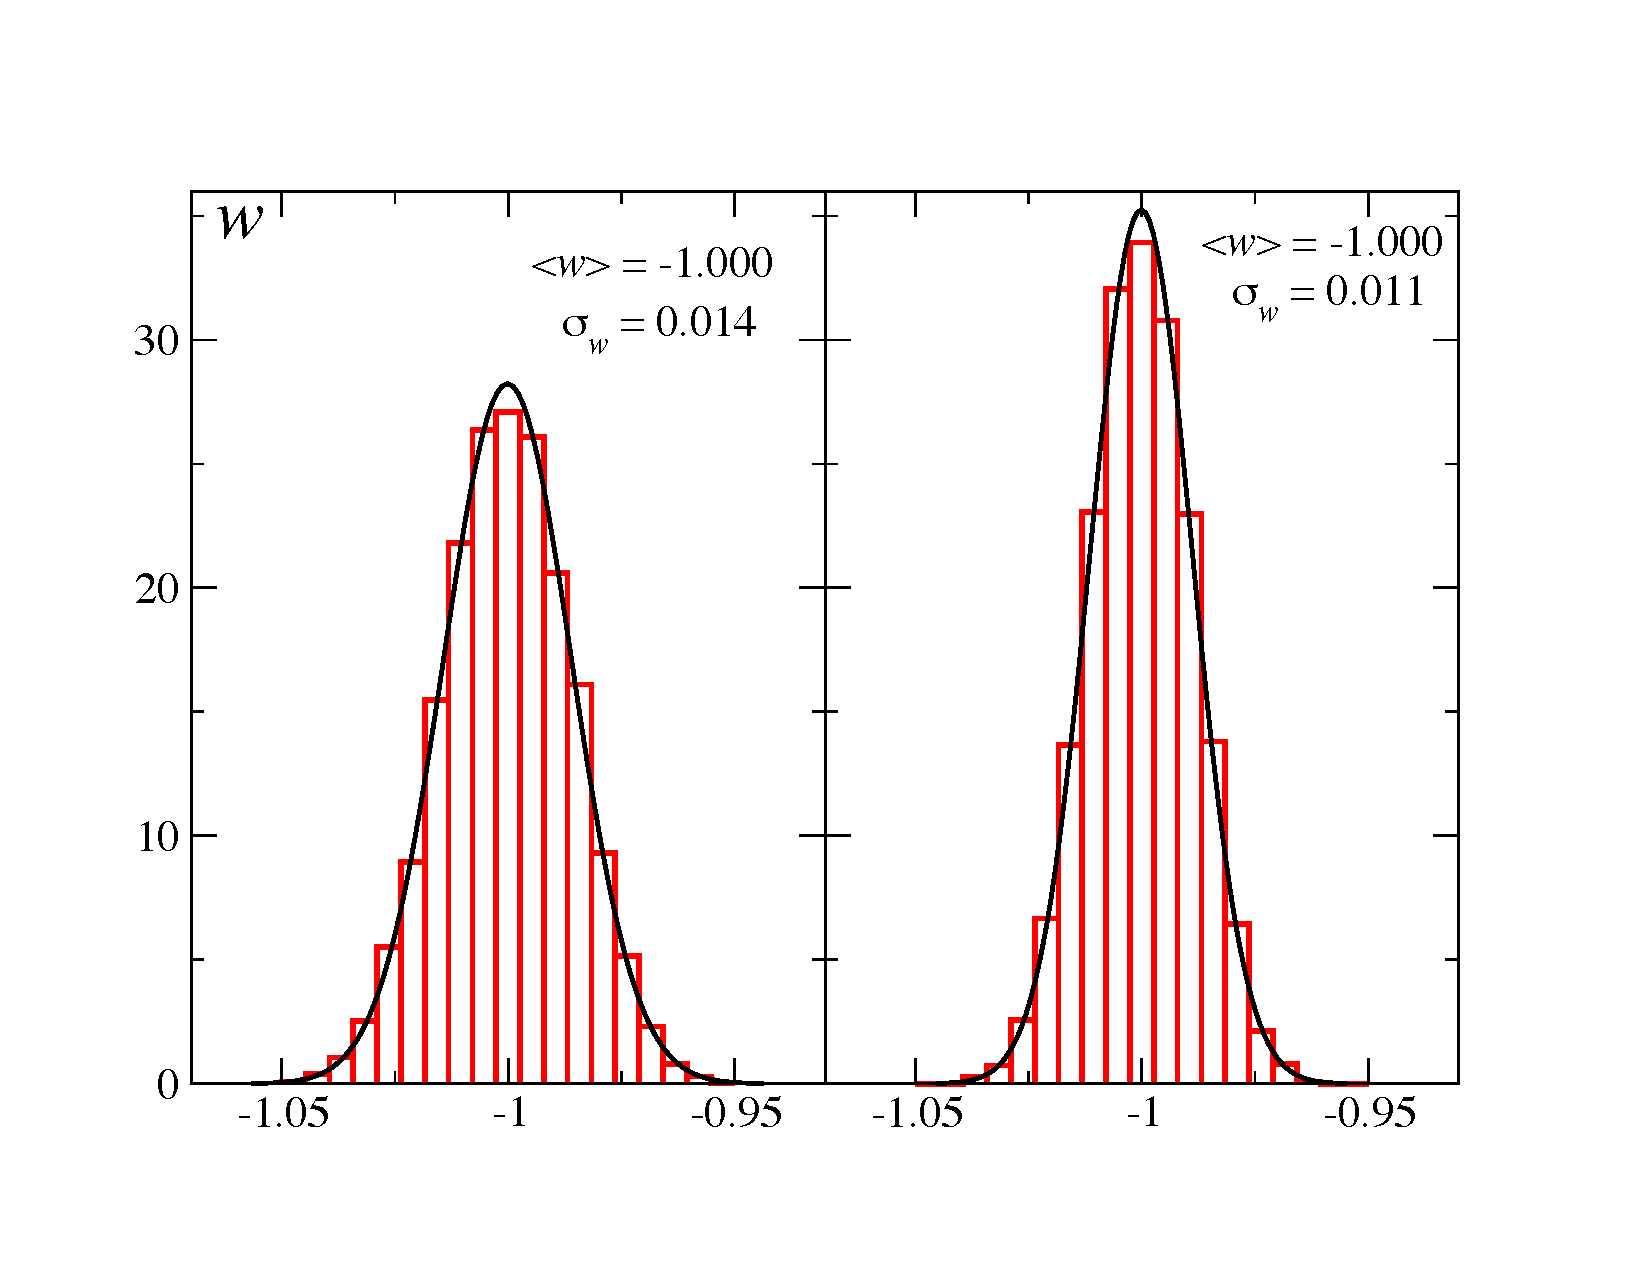
\includegraphics[width=0.45\textwidth]{./Sec_ET_ScienceCase/1params.pdf}
\caption{Same as the Fig.~\ref{fig:fits} except
that one or more of the cosmological parameters are assumed to be
known.  The plot on the left assumes that $\Omega_\Lambda$ is
known to be $\Omega_\Lambda=0.73$, and fits the ``data'' to the 
model with two free parameters $\Omega_{\rm M}$ and $w.$
The fractional 1-$\sigma$ widths in the distribution
$\sigma_{\Omega_{\rm M}}/\Omega_{\rm M}$ and $\sigma_w/|w|$,
are 9.4\% and 7.6\% (with weak lensing errors in $D_{\rm L}$,
left panels) and 8.1\% and 6.6\% (if weak lensing errors
can be corrected, right panels). The plot on the
right is the same but assuming that $w$ is the
only unknown parameter.  The fractional 1-$\sigma$ width of the
distribution $\sigma_w/|w|$ is 1.4\% (with weak lensing errors
in $D_{\rm L}$, left panel) and 1.1\% (if lensing errors can be
corrected, right panel).}
\label{fig:fits2}
\end{figure*}


%\begin{wrapfigure}{r}{0.5\textwidth}
%\vskip -1cm
%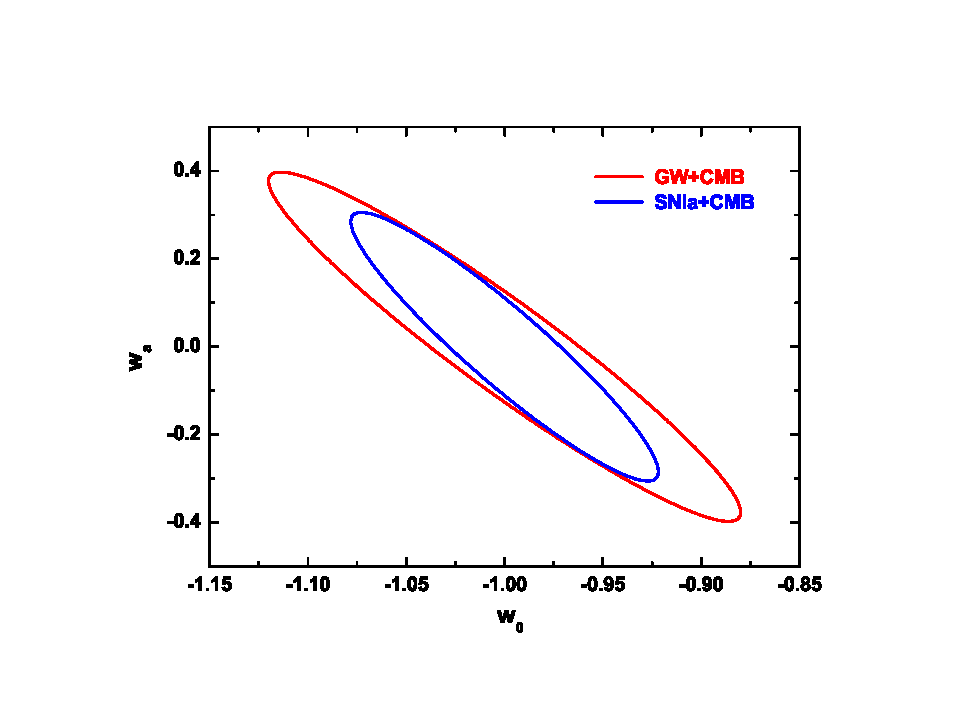
\includegraphics[width=0.5\textwidth]{./Sec_ET_ScienceCase/fc2.pdf}
%\caption{The plot shows the accuracy in $(w_0,w_a)$ obtained from ET observations of binary neutron stars using projected Planck CMB accuracies as a prior for the other cosmological parameters compared to the expected accuracies from SNIa results.}
%\vskip -0.5cm
%\label{fig:cosmofigs}
%\end{wrapfigure}

\paragraph{Effect of unknown orientation and polarization}
In the previous section, our study neglected the effect of different
inclinations of the orbit to the line-of-sight. Varying the inclination
has two distinct effects. On the one hand, as noted in
Ref. \cite{Nissanke:2009kt}, due to the strong correlation between
the luminosity distance and inclination, the estimation of luminosity
distance could get corrupted. On the other hand, binaries that are
not face-on are, in general, elliptically polarized and have a non-zero
polarization angle. Since polarization angle is correlated with the
luminosity distance, there could be further degradation in the
estimation of the luminosity distance.

In this section we will relax the condition that the inclination of the
orbit is precisely known. However, we shall restrict the inclination
of the binary's angular momentum with the line-of-sight to be within
20 degrees. We shall also assume that the radiation is described by
an arbitrary polarization angle. Since the sky position is still assumed known,
this gives us a $7\times 7$ covariance matrix with a revised estimate for the error in the
luminosity distance. As before, we construct catalogues of binary
coalescence events but with the luminosity distance now drawn from
a Gaussian distribution with revised widths. We fit each catalogue
to a cosmological model and then repeat the exercise 5,190 times to
estimate the accuracy with which the various cosmological parameters
can be measured.

As expected, the parameter measurements get worse if we assume two
or more parameters to be unknown.  For instance, errors in the estimation
of $\Omega_{\rm M}$, $\Omega_\Lambda$ and $w,$ are, respectively, $>100\%,$ $24\%$ and
$47\%$ with weak lensing and $>100\%,$ $21\%$ and $43\%$, if weak lensing
can be corrected. Similarly, if $\Omega_\Lambda$ is assumed to be known then
the errors in the estimation of $\Omega_{\rm M}$ and $w$ are, respectively,
$12\%$ and $9.5\%$ if weak lensing is uncorrected for and $11\%$ and
$9.2\%$ if weak lensing can be corrected. However, the results are
more or less the same if the DE EoS parameter $w$ is the only unknown
quantity. Even when the inclination and polarization angles are taken
as free parameters, but inclination angle is restricted to within 20
degrees, the error in the estimation of $w$ is $1.4\%$ with weak lensing
and $1.3\%$ if weak lensing can be corrected.

\paragraph{Variation of dark energy with redshift}
We have seen that the Hubble constant $H_0$ can be measured with high
accuracy using low-redshift sources, after which parameters like $\Omega_{\rm M}$,
$\Omega_\Lambda$, and the DE EoS parameter $w$ can
be determined, where so far we have assumed that the latter is constant. One could
go one step further and use prior information from
{\em e.g.} future Planck CMB measurements to get high-accuracy values for
$(\Omega_{\rm M}, \Omega_\Lambda)$, and then measure the variation of $w$ with
time (see Box~\ref{box:de}). Since CMB data would have a very wide prior on $w$ and its first time derivative,
this would constitute an independent measurement of the latter variables.
%
Allowing for GRB beaming angles of 40$^\circ$, following the procedure
described in Appendix \ref{sec:wandwz} one then finds 
$\Delta w_0 = 0.096$ and $\Delta w_a = 0.30$, which
is comparable to projections from both the SNAP Type Ia supernova and the JDEM Baryon Acoustic Oscillations projects \cite{Zhao:2010}; see Fig.~\ref{fig:cosmofigs}. However, we stress that GW standard sirens are \emph{self-calibrating} and have no dependence on a cosmic distance ladder.


\begin{figure}[h]
\centering
%\vskip 0cm
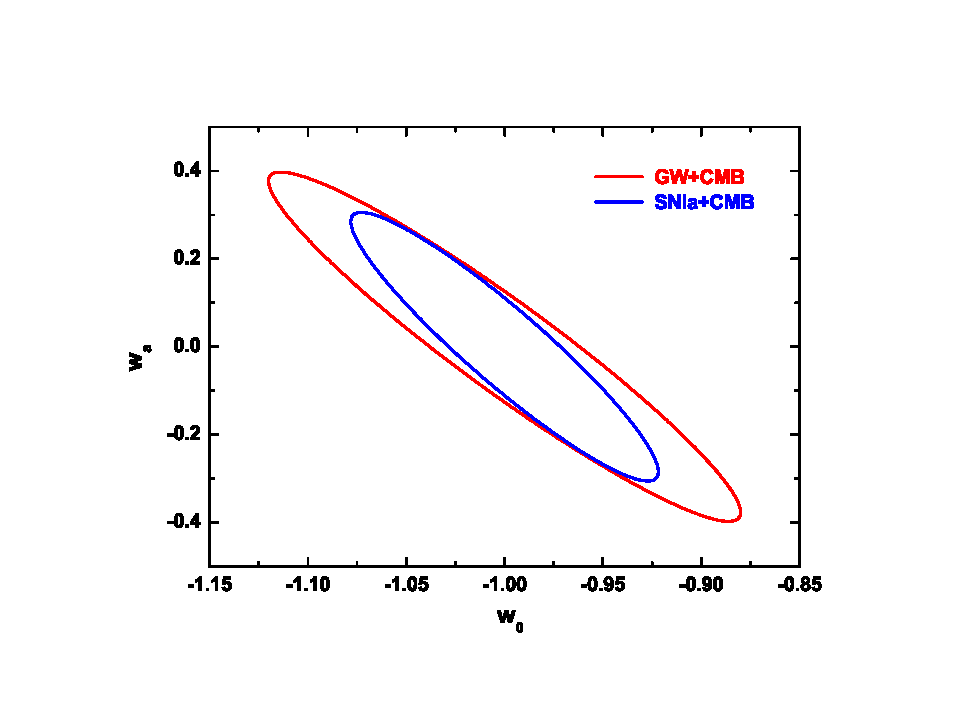
\includegraphics[width=0.5\textwidth]{./Sec_ET_ScienceCase/fc2.pdf}
\vskip -0.4cm
\caption{The accuracy in $(w_0,w_a)$ obtained from ET observations of binary neutron stars using projected Planck CMB accuracies as a prior for the other cosmological parameters, compared to the expected accuracies from SN Ia results.}
\label{fig:cosmofigs}
\end{figure}

\etbox{r}{box:de}
{Variation of $w$ with redshift}
{
Rather than looking at the variation of the dark energy equation of state parameter 
$w$ with time, it is more convenient to consider variation with the scale factor or redshift:
\begin{align}
w(z) &= w_0 + w_a (1-a) + \mathcal{O}\left[(1-a)^2\right] \nonumber\\
     &\simeq w_0 + w_a \frac{z}{1+z}.
\end{align}
Since here we are mostly interested in the later stages of the 
universe's evolution, higher order terms will be ignored. With a 
redshift dependent $w(z)$, the Hubble parameter as a function of redshift 
becomes
\begin{equation}
H(z) = H_0\,\left[\Omega_{\rm M}(1+z)^3 + \Omega_\Lambda\,(1+z)^{3(1+w_0+w_a)}e^{-3 w_a z/(1+z)}\right],
\end{equation}
and luminosity distance is still related to the Hubble parameter as
\begin{equation}
D_{\rm L}(z) = c(1+z)\int_0^z \frac{dz'}{H(z')}.
\end{equation}
With a catalogue of sources with accurately measured luminosity distances 
$D_{\rm L}$ and corresponding redshifts, the above relation can be used to
deduce $w_0$ and $w_1.$ See Appendix  \ref{sec:wandwz} for a discussion of how
the errors are computed.
}

\paragraph{Open problems}

The results of our simple simulation are quite encouraging but further
work is needed to confirm the usefulness of GW standard sirens in
precision cosmology. Let us mention some that are currently being purused.
Spins of component stars can be legitimately neglected in the case of
neutron stars (and hence in BNS) but not for black holes and the
modulation in the signal caused by the spin of the black hole
can improve parameter accuracies. We assumed, for simplicity, that
all our systems are BNS systems with masses $(1.4,\,1.4)M_\odot.$
In reality, the catalogue will contain a population consisting of a
range of NS and BH masses. A more realistic Monte Carlo simulation
would draw binaries from the expected population rather than the same system,
some of which (more massive and/or equal-mass systems) would lead to
better, but others to worsened, parameter accuracies.
The signal contains additional features, such as other harmonics
of the orbital frequency than the second harmonic considered in this
work and the merger and ringdown signals. Both of these are important
for heavier systems and could potentially reduce the errors.
These factors are currently being taken into account to
get a more reliable estimation of the usefulness of ET in precision
cosmography.


\FloatBarrier
\subsubsection{Cosmological evolution of compact object populations}

The calculation of the coalescence rate as a function of the redshift must take into account the following factors: the star formation rate history $SFR(z)$, the binary fraction $f_b(z)$, the formation efficiency of a given type of binary, i.e.\  the fraction of number of binaries that lead to formation of coalescing compact object binary, and their distribution of merger times. These quantities may depend on redshift since the stellar populations evolve with cosmic time.  Let us examine the effects of  evolution of each of these factors.


The star formation rate is known to increase strongly to the redshift 
$z=2$, and there is a debate about its behavior for higher redshifts. 
At redshift $z=2$, the star formation is estimated to be a factor of 10   
larger \cite{Heavens:2004sr} than the present value at $z=0$. 
% {\bf Present a figure here a discuss with references.}

The distribution of merger times can be estimated either by analyzing the present population of compact binary objects or by involving the population synthesis. The first approach is limited to dealing with BNSs, and suffers from small number statistics. The second involves several uncertainties due to parametrization of  binary evolution. However the two approaches yield similar results. The distribution of merger times for BNSs can be well approximated by a distribution $\propto t^{-1}$. The lower cutoff for the BNS systems lies somewhere between 10 and 100 Myrs. The population synthesis  leads to similar conclusions about the distribution of merger times for NSBH and BBH systems, however the low time cutoff may probably lie higher.

% Figures -

The main factor that may affect the evolution of the binaries as a function of redshift are the changes in the distribution of metallicity.  Metallicity strongly affects the mass loss rate in stars, and hence has a strong influence on  the mass spectrum of compact objects. The lower the metallicity, the higher the maximum mass of a BH that may be formed in the course of stellar evolution. This leads to a stabilization of mass transfers and therefore to an increase in the formation rate of compact object binaries.

% {\bf
%Show the plots as a function  of Z.  }

%{\ bf Show plots of metallicity evolution.}

Taking together the above factors we see that there are several reasons why the coalescence rate should increase strongly as we go to redshifts of $z=1$--2. First, the local star formation rate increases and the overall amount of binary formation is larger. Second, the typical delay times for the BNS systems are low therefore their merger rate density will roughly follow that of the SFR. In the case of NSBH or BBH systems the typical delay times between formation and coalescence may be as large as 1--3 Gyrs. This delays the peak of coalescence rate density with respect to the star formation rate. Thus, the delays are significant but not crucial. Third, the metallicity evolution may lead to higher compact object formation rate for high redshifts, and the formation of larger number of massive BBH systems.

This consideration can be put into detailed numerical codes to yield predictions about the rates. However, even without such strong numerical support one can readily estimate with a ``back of the envelope calculation'' that the ratio of the coalescence rate (per unit volume per unit time) to the local one should be at least a few.  The local coalescence rate can only be estimated with observations, since neither the observational not the indirect approach mentioned earlier can yield an estimate of the rate with an accuracy better that an order of magnitude.

The Einstein Telescope will provide a large sample of  coalescences with the precisely measured masses and redshifts.  This will be an extremely valuable tool for analysis of the cosmic compact object formation history.  The measurement of their masses will yield information on the metallicity evolution as well as the evolution of the most massive stars. The Einstein telescope will yield a cosmic compact object census up to redshift $z=2$, and will yield information about BHs and NSs formed at even earlier epochs because of the delays between formation and coalescence.


There are two distinct routes to form BH binaries. % {\bf Stas: Bulik to correct this part}
The first, conventional way, is to start with a binary system of two main sequence stars and trace their
evolution. There are several big uncertainties in this process. The first one
is the initial mass ratio function: what is the distribution of the mass ratio
in the binary of two main sequence stars, how does it depend on the metallicity
and spectral type. The second, and probably the biggest uncertainty, is related
to the ``common envelope'' evolution, where the NS (or BH) and the helium core
are exposed and evolve in the gaseous environment of the star. In this stage
the NS or BH could merge with the helium core %% on the time scale ... ,
and not form a binary. The third uncertainty is related to the direction and magnitude of the
kick exerted on the newly born BH from the  asymmetric  supernova  explosion.
All the above is reflected in the uncertainties on the rate of such binaries \cite{LPP:LRR,BB:1999}.


The BH binaries could also be formed in a dense environment such as galactic nuclei.
In galaxies with SMBHs ($M < 10^7\, M_{\odot}$), the relaxation time is less than a Hubble
time, and a steep cusp of stars and stellar mass BHs can be formed. BHs, as massive,
compact objects, will segregate into the central $\approx 1$ pc region. Other dense regions include
massive globular clusters and nuclear star clusters in the centres of low-mass galaxies
which may not have SMBH. The densities in those regions are high enough to have multiple
encounters, with formation and/or hardening of BH binaries.

% {\bf TO DO: Bursts coming from parabolic encounters (Kocsis et al The Astrophysical Journal, Volume 648, Issue 1, pp. 411-429). Conditions under which we could form the tight binaries.
% Galactic nuclei with SMBH: based on O'Leary et al MNRAS, Volume 395, Issue 4, pp. 2127-2146, low mass galaxies without SMBH: based on Baumgardt et al; Miller \& Lauburg ApJ 629, 917 (2009).
% Resonant interaction (Kozai). DIstribution of the eccentricity in those binaries as they enter the
% detector band.}
\subsubsection{Reconstruction of the evolution of compact binary 
coalescence rates by ET}

The rate at which NSs and BHs coalesce at different redshifts can 
provide indirect but extremely valuable insights into the star 
formation rate (SFR). ET will be able to distinguish between 
coalescence rate predictions from different SFR models and hence 
provide indirect evidence for history of star formation at high 
redshifts. Considering that BNS coalescences are expected to be 
the most abundant, they are the best ``trackers" of SFR, and these 
are the events we will focus on.

The rate (per unit time and per unit comoving volume) at which 
BNS systems are observed to coalesce at redshift $z$ in our frame, 
denoted $\dot\rho^0_c(z),$ can be written as \cite{Regimbau:2009} 
\begin{equation}
\dot{\rho}^0_c(z) = \dot{\rho}^0_c(0) 
\frac{\dot{\rho}_{\ast,c}(z)}{\dot{\rho}_{\ast,c}(0)}.
\label{eq:rates}
\end{equation}
Here $\dot{\rho}^0_c(0)$ is the coalescence rate in our frame at the 
current epoch, and $\dot{\rho}_{\ast,c}$ relates the past star 
formation rate to the rate of coalescence:
\begin{equation}
\dot{\rho}_{\ast,c}(z) = \int \frac{\dot{\rho}_\ast(z_f)}{(1+z_f)} P(t_d) dt_d,
\end{equation}
where $\dot{\rho}_\ast$ is the SFR itself, $z_f$ is the redshift at 
which the {\em progenitor binary forms,} $z$ is the redshift at which the 
{\em compact binary coalesces,}. These redshifts are connected by the {\em delay time}  $t_d$ which is the sum of the time from initial binary
formation to evolution into compact binary, plus the merging time
$\tau_m$ by emission of gravitational waves.  The delay is also the
difference in lookback times between $z_f$ and $z$:
\begin{equation}
t_d = t_{\rm LB}(z_f) - t_{\rm LB}(z) = \frac{1}{H_0}
\int_z^{z_f} \frac{dz'}{(1 + z')H( z')}\,
\end{equation}
Its probability distribution $P(t_d)$  has been estimated as
\begin{equation}
P(t_d) \propto \frac{1}{t_d}\qquad \mbox{for}\quad t_d > \tau_0,
\end{equation}
where $\tau_0$ is some minimum delay time. 
Thus, the limits in the integral
(\ref{eq:rates}) vary from $\tau_0$ to $\infty,$ with no contribution from
the upper limit (binaries that take infinitely long to coalesce contribute
nothing to the rate).  As in Regimbau and Hughes, \cite{Regimbau:2009} we 
assume $\tau_0 \sim 20$ Myr,  corresponding roughly to the time it takes for massive binaries to evolve into two neutron stars.
The coalescence rate per unit redshift as 
observed in our local Universe is found by multiplying 
$\dot{\rho}^0_c$ by the gradient of comoving volume:
\begin{equation}
\frac{dR^0_c}{dz} = \dot{\rho}^0_c(z) \frac{dV_c}{dz}(z).
\end{equation}


We may now ask how well ET will be able to discriminate between 
different SFR models $\dot{\rho}_\ast(z)$ through differences in 
the resulting observed BNS coalescence rates $\dot{\rho}^0_c(z)$. To 
this end we consider four different models:
\begin{itemize}
\item Hopkins and Beacom \cite{sfr-HopkinsBeacom2006}: This model is 
based on an observational compilation, placing lower bounds on SFR using the 
evolution of stellar mass density, metal mass density, and supernova rate 
density, and an upper bound using Super-Kamiokande results for the 
electron antineutrino flux from core-collapse supernovae;
\item Nagamine et al.~\cite{Nagamineetal06}: This is an approach comparing and 
combining results from direct observations, a model using local fossil 
evidence at $z \sim 0$, and theoretical \emph{ab initio} models;
\item Fardal et al.~\cite{Fardaletal07}: Fardal et al.\, use a model 
involving a new proposal for the initial mass function with a view 
on reconciling SFR predictions with the total extragalactic background 
radiation;
\item Wilkins et al.~\cite{Wilkinsetal08}: This model is based on 
stellar mass density measurements together with a new ansatz for the 
initial mass function.
\end{itemize}
The merger rates predicted by these models are plotted in Fig.\,\ref{fig:ratesrecovery}.

\etbox{r}{box:merger rates}
{History of star formation rate from binary coalescence rate}
{
To evaluate how well ET can measure the merger rate of compact
binaries we start offf with a catalogue of BNS coalescences as
described in Box \ref{box:cosmo params}.
%Given a fiducial cosmological model, one can associate a luminosity 
%distance $D_{\rm L}(z)$ with each simulated source. In a spatially flat 
%Friedman-Robertson-Walker universe, this relationship takes the form
%given in Eq.\,(\ref{DLgeneral}):
%\begin{equation}
%D_{\rm L}(H_0, \Omega_{\rm M}, \Omega_{\rm \Lambda}, w; z) = \frac{1+z}{H_0} \int_0^z \frac{dz'}{\left[\Omega_{\rm M}(1+z')^3 + \Omega_{\rm \Lambda}(1+z)^{3(1+w)}\right]^{1/2}},
%\label{DL}
%\end{equation}
%where $H_0$ is the Hubble parameter at the current era, $\Omega_{\rm M}$ 
%is the density of matter normalized by the critical density, 
%$\Omega_{\rm \Lambda}$ the density of DE (similarly normalized), and $w$ 
%is the equation-of-state parameter of DE. 
%\\[5pt]
The luminosity distances measured from the GW signal, $\hat{D}_{\rm L}$, will be 
different from the true distance due to (i) the noise in the detector, and 
(ii) (de)magnification as a result of weak gravitational lensing. 
Thus, with each source we associate a ``measured" luminosity distance
\begin{equation}
\hat{D}_{\rm L}(z) = D_{\rm L}(z) + \delta D_{\rm L}(z),
\label{DLmeasured}
\end{equation}
where $\delta D_{\rm L}(z)$ is drawn at random from a Gaussian distribution 
with a spread given by
\begin{equation}
\Delta D_{\rm L} = (\sigma_{\rm ET}^2 + \sigma_{\rm WL}^2)^{1/2}.
\label{disterr}
\end{equation}
We treat the errors $\sigma_{\rm ET}$ and $\sigma_{\rm WL}$ 
in the same way as in Box \ref{box:cosmo params}.
%The contribution $\sigma_{\rm ET}$ is due to detector noise while 
%$\sigma_{\rm WL}$ results from weak lensing. Note that 
%$\Delta D_{\rm L}$ will depend not only on redshift but also on sky 
%position and the orientation of the orbital plane. As a rule of thumb, 
%one can take $\sigma_{\rm ET}/D_{\rm L} \simeq 1/\rho$, and for the 
%weak lensing error we assume $\sigma_{\rm WL}/D_{\rm L} = 0.05 z$.
%\\[5pt]
%Having distributed sources as described above and associated measured 
%luminosity distances to them, we have a simulated ``catalogue" of 
%detected inspiral events.  
Using the fiducial cosmological model, the measured luminosity distances 
$\hat{D}_{\rm L}(z)$ can be inverted to obtain measured redshifts 
$\hat{z}$ by inverting Eq.~(\ref{DLmeasured}).  In doing so we choose our 
fiducial cosmological model such that $H_0 = 70\,\mbox{km}\mbox{s}^{-1}
\mbox{Mpc}^{-1}$, $\Omega_{\rm M} = 0.27$, $\Omega_{\rm \Lambda} = 0.73$, 
and $w = -1$.
The recovered redshifts are then binned to obtain a recovered rate 
distribution $d\hat{R}^0_c/dz$. 
By doing this for a large number of different simulated catalogues 
(say, 1000 catalogues), one can compute an average and a 1-sigma spread 
for the number of sources in each recovered redshift bin.
\\[5pt]
To check how well ET will be able to distinguish between different coalescence 
rate predictions, we can fold in the anticipated efficiency $\epsilon(z)$, i.e.\  the 
fraction of coalescences at a given redshift that survive the SNR 
cut $\rho > 8$. The efficiency is 
essentially 100\% up to $z \simeq 0.7$, after which it starts to drop rather quickly. 
Beyond $z \simeq 3.5$ no signals can be seen even when optimally positioned 
and oriented. The efficiency can be folded into the recovered rate distribution:
\begin{equation}
\left[ \frac{dR^0_c(z)}{dz} \right]_{\rm recovered} = 
\epsilon(z)^{-1} \frac{dR_c^0(z)}{dz},
\end{equation}
where $dR_c'/dz$ is the distribution inferred from binning the measured redshifts.
}
Box \ref{box:merger rates} discusses how ET could be used to measure
the merger rate as a function of redshift.
In a nutshell, simulated BNS sources are placed according to the 
coalescence rates $\dot{\rho}^0_c(z)$ inferred from the four models 
using their proposed $\dot{\rho}_\ast(z)$, with a minimum delay time 
$\tau_0 = 20$ Myr. Sources are positioned uniformly in the sky; an SNR 
threshold is imposed such that a source is disregarded unless its SNR is 
$\rho > 8$. the coalescence rate at the current epoch was (very) conservatively set 
to be $\dot{\rho}^0_c = 0.03\,\mbox{Mpc}^{-3}\mbox{Myr}^{-1}$, 
in which case between $\sim 150$,000 and $\sim 275$,000 sources survive 
the SNR cut, depending on the SFR model. Note that this local coalescence 
rate will most likely already be measured by Advanced LIGO and Virgo, so 
that we may consider it a known quantity in the context of ET.

\begin{figure*}
\begin{center}
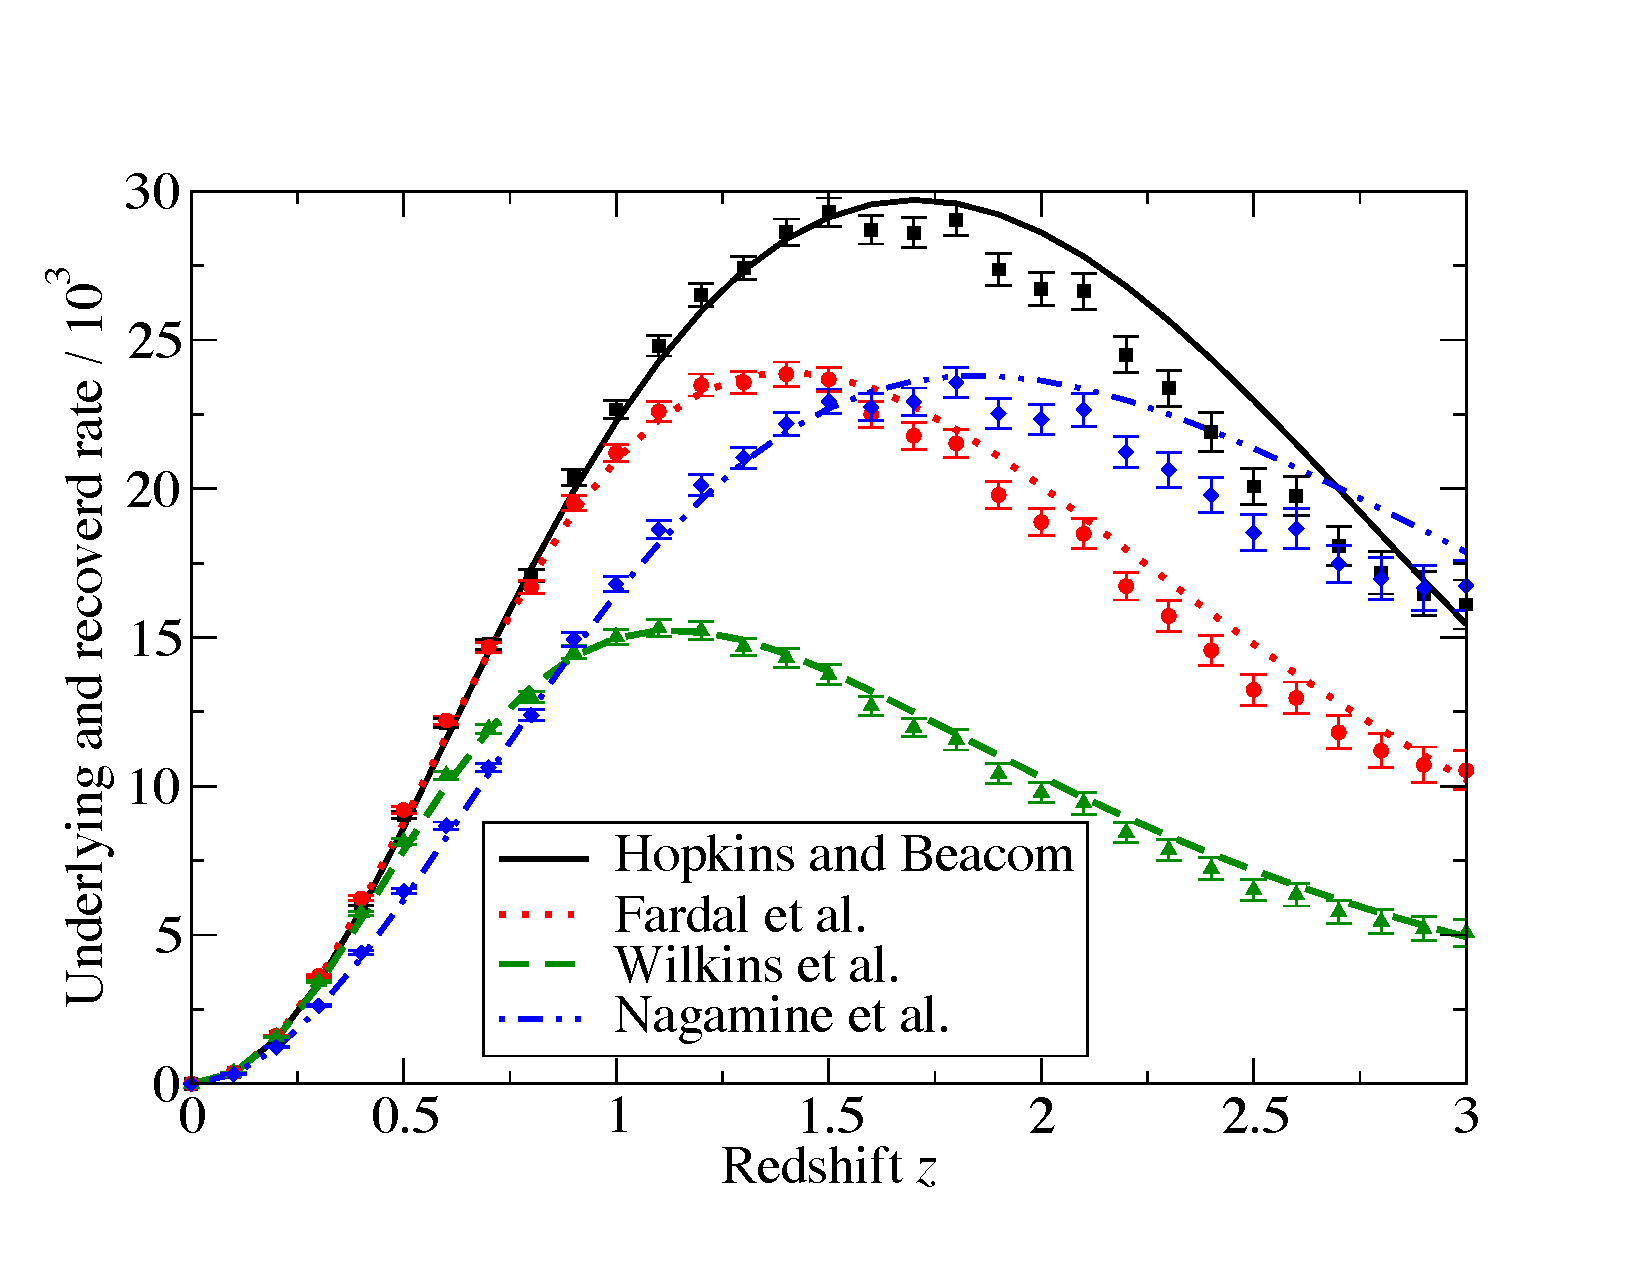
\includegraphics[width=0.5\textwidth]{./Sec_ET_ScienceCase/rates.pdf}
\caption{True and recovered coalescence rates (taking into account 
detection efficiency) for the models of Hopkins and Beacom 
\cite{sfr-HopkinsBeacom2006} (solid black line), Fardal et al.~\cite{Fardaletal07} 
(dotted red line), Wilkins et al.~\cite{Wilkinsetal08} (dashed green line), and 
Nagamine et al.~\cite{Nagamineetal06} (dot-dot-dashed blue line). The lines 
are the true rates, the symbols give the number of measured 
coalescences in a redshift bin, error bars denoting a 2-sigma 
spread in recovered rates.}
\label{fig:ratesrecovery}
\end{center}
\end{figure*}
Fig.~\ref{fig:ratesrecovery} shows both the underlying rates 
$dR^0_c(z)/dz$ and the recovered rates, with 2-sigma spreads, for the four SFR 
models considered. First we note some systematic effects due to uncertainties 
in the redshift measurements:
\begin{itemize}
\item At small redshifts ($z \lesssim 1.5$), the recovered rate distribution is shifted very slightly to the left with respect to the underlying distribution. This is because of higher-redshift events ending up in lower redshift bins due to measurement errors. The effect is not compensated by lower redshift events ending up in higher redshift bins, because at lower redshifts the spread in measured redshift is smaller.
\item At intermediate redshifts ($1.5 \lesssim 3$) the true coalescence rate is being underestimated (despite having folded in efficiency loss) because of events ending up in both higher and lower measured redshift bins;
\item Beyond $z \simeq 3.5$ the recovered rate diverges, because there are still \emph{measured} redshift values there, but the efficiency $\epsilon(z) \rightarrow 0$.
\end{itemize}
We see that ET can easily distinguish between the four models we took from recent literature. Generally, two models for BNS coalescence rates can be distinguished from each other if over at least one $\Delta z = 0.1$ redshift bin at $z \lesssim 1.5$, the number of sources in the bin differs by more than a few percent.


\subsubsection{Intermediate mass black holes}

The existence of IMBHs with masses in the range
$10^2 - 10^4\,M_\odot$ has not yet been corroborated observationally, but these
objects are of high interest for astrophysics. Our understanding of the formation and
evolution of supermassive BH, as well as galaxy evolution modeling and
cosmography would dramatically change if an IMBH were to be observed. From the
point of view of traditional electromagnetic astronomy, which relies on the monitoring of
stellar kinematics, the direct detection of an IMBH seems to be rather far in the future.
However, the prospect of the detection and characterization of an IMBH has good chances in
lower-frequency GW astrophysics, in particular with ET. The detection and characterization of
a binary containing an IMBH would corroborate the existence of such systems and
provide a robust test of general relativity through tests of the BH
uniqueness theorem (see subsection~\ref{subsubsec:uniquenesstheorem}).

Signals from IMBH binaries can start in the band of LISA, and sweep through to the
ET band, allowing us to observe different aspects of the coalescence event, as illustrated
in Fig.~\ref{fig:IMBH}. For ET, a lower cut-off frequency of 1\,Hz was assumed.

\begin{figure}[tb]
\begin{center}
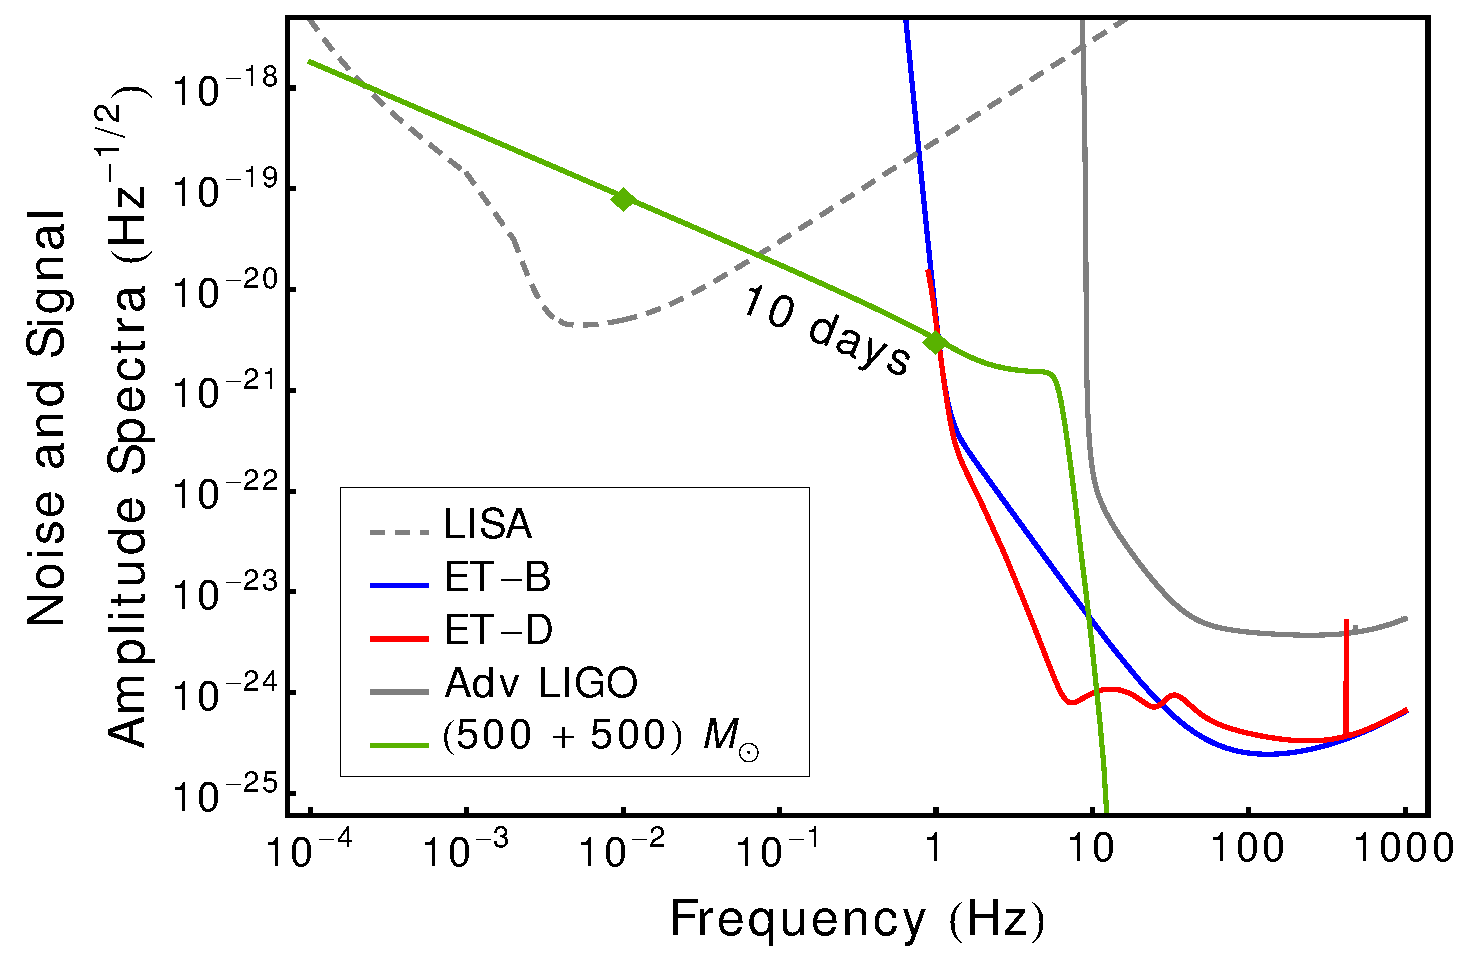
\includegraphics[width=0.49\textwidth]{./Sec_ET_ScienceCase/IMBH1.pdf}
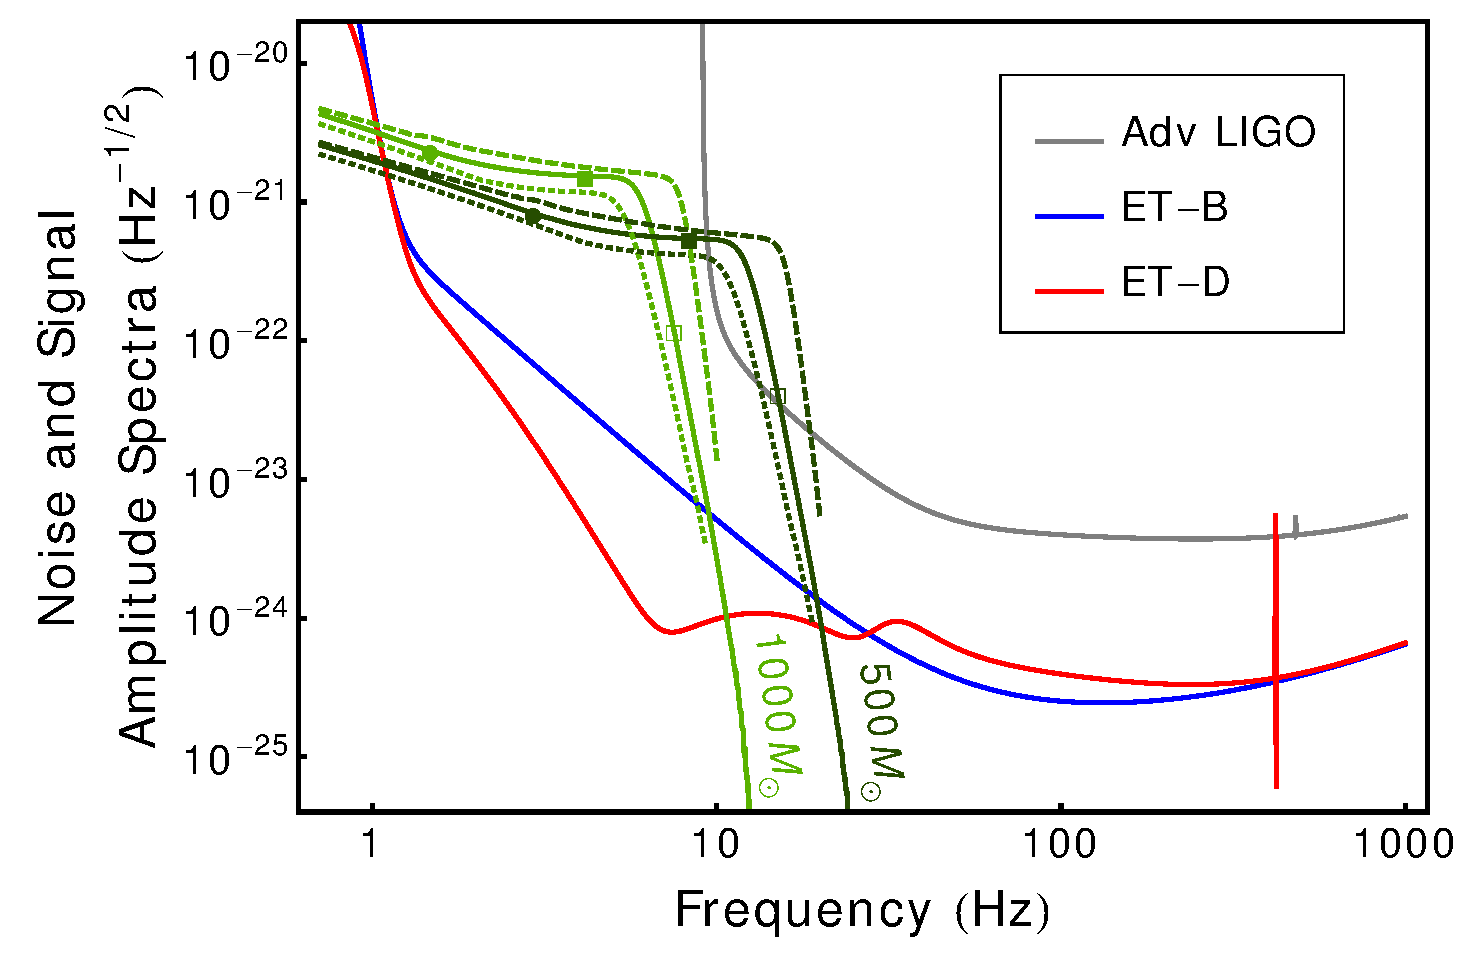
\includegraphics[width=0.49\textwidth]{./Sec_ET_ScienceCase/IMBH2.pdf}
\end{center}
\caption{Amplitude spectra of IMBH binaries compared to ET sensitivity
curves. Left: Different aspects of the inspiral, merger and ringdown 
signal from a binary IMBH with {\em intrinsic} masses $(500,500)\,M_\odot$ 
at $z=2$ can be studied as the system passes in 10 days from the LISA band into 
the ET band. Observed masses are redshifted by a factor $(1+z)$ compared
to physical masses, so this system would be seen to consist of two 
IMBHs each of mass $1500\,M_\odot$. 
Right: Signals from IMBH binaries of intrinsic total mass as labelled by
the curves, all at a redshift of $z=2$ and so have observed total mass 
that is larger by a factor $3.$ The solid lines are for equal mass, 
non-spinning binaries, dashed lines for binaries with equal masses 
and dimensionless spins $\chi = 0.75$ and the dotted lines for 
non-spinning binaries with mass ratio $m_1/m_2=3$. ET's better low
frequency sensitivity is key to observing the intermediate BHs which
might have triggered formation of galaxies and large scale structure.
ET should be able to see $100$-$1000\,M_\odot$ binary IMBH mergers at redshifts
$z\sim 12$-$3$ (see Fig.\,\ref{fig:ET_range}).
}
\label{fig:IMBH}
\end{figure}

\subsubsection{Black hole seeds and galaxy formation}

% \ledby{Gair}
It is widely accepted that the massive black holes (MBHs) found in the centres of many galaxies grow from initial seeds through the processes of accretion and following mergers between their host DM halos. However, little is known about the seeds from which these BHs grow. Open questions include: What are their masses? Where are they? How and when did they form? Current observations are consistent with both \emph{light seed} scenarios, in which $\sim100M_{\odot}$ BH seeds form at redshift $z \approx 20$ from the collapse of Population III stars~\cite{svh,madau01}, and \emph{heavy seed} scenarios, in which BH of mass $\sim10^5\,M_{\odot}$ form from direct collapse of dust clouds~\cite{KBD,BVR}. Mergers between MBHs in merging DM halos will generate GWs. These are a major source for LISA~\cite{PPA}, but LISA will only see mergers with total mass $\gtrsim 10^3\,M_{\odot}$. LISA can therefore probe BH seeds only in the heavy seed scenario and does not have the power to discriminate between the light and heavy scenarios.

ET will have sensitivity in the $1$--$50$\,Hz band
in which GWs from mergers involving
$\sim10$--$100\,M_{\odot}$ BHs will lie. It will therefore
provide complementary information to LISA and could directly observe
the first epoch of mergers between light seeds. Present estimates,
based on Monte Carlo simulations of galaxy merger
trees~\cite{vhm,vsh}, suggest ET could detect
between a few and a few tens of seed BH merger events over
three years of operation~\cite{sgmv09a}. Several of these events will
be at high redshift, $z\sim5$, by which time it is unlikely that
$100\,M_{\odot}$ BHs could have formed by other routes. ET and
LISA in conjunction probe the whole merger history of DM
halos containing BHs in the $10$--$10^6\,M_{\odot}$ range, which
will provide detailed information on the hierarchical assembly of
galaxies. ET is able to measure the distance to a GW source, with 
one additional non-colocated interferometer, to $\sim40\%$ precision 
and the redshifted total mass of the system to $\lesssim 1\%$.
Using a concordance cosmology, this distance estimate can be used 
to deduce the redshift with comparable accuracy and so it should be 
possible to say that the $z \approx 5$ events are of \emph{low mass} 
and at \emph{high redshift}, and therefore are convincing candidates 
as Population III seed mergers.

Just one detection by ET will rule out the heavy seed model. With several detections, we will be able to make statements about Population III seed BH properties, such as their mass distribution, their early accretion history etc.~\cite{sgmv09a}. These observations cannot be made be any other existing or proposed detector --- it is science that is unique to ET. Such observations will be vital to our understanding of the assembly of structure in the Universe, and of the close link between BHs residing in the centres of galaxies and their hosts~\cite{svh}.


\subsubsection{Primordial gravitational waves}
\label{cosmo_stochastic}

The cosmological stochastic background of GWs \cite{Allen1997} is a unique window on the very early Universe, because gravitational radiation propagates uninterrupted to us from cosmic events at the highest temperatures and densities, potentially up to the GUT scale of $10^{16}\,$GeV. The detection of any such background would have huge consequences for fundamental physics, possibly giving us direct indications of inflation, phase transitions or formation of topological defects. A stochastic confusion background of GW from very distant astrophysical sources may also contain significant information on the populations and evolution of the sources.  As shown in Figures~\ref{fig:cosmo_stochastic} and \ref{fig:astro_stochastic}, many types of cosmological stochastic background are potentially above the ET sensitivity curve. It may also be possible to extract information about the cosmological events that produced GW if an observed spectrum has some characteristic shape.

Primordial GW backgrounds are broadly of two types: wide-band, where $\Omega_{\rm gw}(f)$ is approximately constant over a large range of frequency; and peaked, where $\Omega_{\rm gw}$ varies strongly over $f$ reaching a maximum at $f_{\rm peak}$. Wide-band sources are processes that extend over a large range of the cosmological scale factor $a(t)$, such as inflation and cosmic string evolution. Both these sources depend on unknown fundamental physics, and also have an approximate scaling symmetry. The detectability of a ``flat'' background spectrum depends only on the value of $\Omega_{\rm gw}$ at a nominal frequency of $10\,$Hz.

%
\begin{figure}[p]
\centering
\vskip -0.2cm
\includegraphics[width=0.64\textwidth]{./Sec_ET_ScienceCase/landscape_DSD}
\caption{Possible backgrounds of primordial stochastic GW at Advanced LIGO and ET.
%The detector curves $\Omega_{\rm min}h^2(f)$ assume an observation time of 1 year, bandwidth $\delta f = f$ and a detection sensitivity $S/N=2.56$. The detector topology assumed for Advanced LIGO is two coincident coaligned $90^\circ$ interferometers, for ET two $60^\circ$ interferometers placed on an equilateral triangle, one rotated by $120^\circ$ relative to the other. OR:
%Left 
The sensitivity curves correspond to an observation time of 1 year, $S/N$ of $2.56$, and co-located but not necessarily coaligned detectors (see end of Section~\ref{source_stochastic}). 
Models and parameter values are described in the main text. Data for tachyonic preheating and decay of SUSY flat directions were provided by J.-F.~Dufaux; for phase transitions between metastable SUSY vacua, by N.\,J.~Craig; the cosmic string GW spectra are based on a calculation of X.~Siemens {\it et al}.\ \cite{Siemens:2006yp}.
}
\label{fig:cosmo_stochastic}
\end{figure}

\begin{figure}[p]
\vskip -0.4cm
\centering
\vskip -0.3cm
\hskip 0.55cm
\includegraphics[width=0.72\textwidth]{./Sec_ET_ScienceCase/landscape-agb.pdf}
\vskip -0.3cm
\caption{Energy density in GW due to background created by astronomical sources: magnetars (minimal detectable prediction (ET-B) in continuous cyan and model when the spin-down is purely gravitational in dashed cyan), normal radio pulsars assuming a mean ellipticity of $10^{-6}$ and initial distributions from ~\cite{2011arXiv1103.1856G} in yellow, binary neutron stars in black, dynamical bar modes in proto NS in orange, r-modes assuming that $1 \%$ of newborn neutron stars cross the instability window in green, Pop II core collapse to NS (model of~\cite{Ott:2006}) in purple and to BH (model D5a of~\cite{Sekiguchi:2005}) in brown. ET sensitivity curves are as in Fig.~\ref{fig:cosmo_stochastic}.
}
\label{fig:astro_stochastic}
\end{figure}
%

\paragraph{Wide-band sources: inflation and strings}

%\paragraph*{Inflation}
%\

\noindent There are many models of inflation, but they share a few essential features: exponentially expanding the scale factor in a short time; sourcing primordial density perturbations with amplitude $\mathcal{O}(10^{-5})$ and an approximately Harrison-Zeldovich (scalar spectral index $n_s\simeq 1$) spectrum; and reheating the Universe to at least the temperature required for primordial nucleosynthesis (order of $10\,$MeV).
%(A considerably higher temperature $T \geq \mathcal{O}(100)\,$GeV is required for generation of most types of dark matter and for baryogenesis.)
%In standard scenarios the scale factor is an approximately exponential function of time over several tens of e-folds.
%The time translation symmetry during inflation maps to a scaling symmetry of the spectrum: perturbations generated earlier (later) are inflated to larger (smaller) scales but are otherwise (nearly) identical.

Tensor perturbations generated during inflation can be described by an amplitude and spectral index $n_t$. Since their evolution over cosmological time is similar to scalar perturbations, the {\em tensor-to-scalar ratio}\/ $r$ is a useful measure. This ratio is sensitive to the ``energy scale of inflation'' $V^{1/4}$ via an approximate relation
%, or the Hubble rate during inflation,
$V^{1/4} \simeq (1.8 \times 10^{16}\,{\rm GeV})(r/0.07)^{1/4}$ \cite{Lyth:1996im}. In single-field models, the value of $r$ also indicates the minimum distance the field travels during inflation in Planck mass units via $\Delta \phi/M_{P} \simeq 0.46(r/0.07)^{1/2}$.
%For a ``flat'' spectrum $\Omega_{\rm gw}(f)=\mathrm{const.}$ the conversion is $\Omega_{\rm gw}(f)=$(some function of $r$). Current observational bound on $r$ from CMB (+BAO, SN), at frequencies enormously smaller than any GW detector could probe, is $0.22$. Planned experiments should take this down to few times $0.01$. The bound from BBN on the {\em total}\/ $\Omega_{\rm gw}$ is $10^{-5}$ from BBN.

%- Pulsar timing bound: $\Omega_{\rm gw}(f=4.4\times 10^{-9}\,{\rm Hz}) < 4.8\times 10^{-9}$ (Kaspi 1994).

For a scale-invariant spectrum ($n_s=1$, $n_t=0$) the CMB determination of the scalar amplitude $S \sim 10^{-10}$ together with the current bound $r\lesssim 0.2$ translates to a very small value $\Omega_{\rm gw}(f)\lesssim 10^{-15}$ for all frequencies accessible to interferometers \cite{Turner:1996ck,Kuroyanagi:2008ye}. However, since the CMB bounds apply at $f\sim 10^{-18}\,$Hz, a positive spectral index $n_t$ could change the picture \cite{Grishchuk:1996ek}: we have $\Omega_{\rm gw}(10\,{\rm Hz}) = (10^{19})^{\bar{n}_t}\Omega_{\rm gw}(10^{-18}\,{\rm Hz})$, where $\bar{n}_t$ is the averaged spectral index between these two frequencies \cite{Boyle:2007zx}. In Fig.~\ref{fig:cosmo_stochastic} we plot the possible signal for $r=0.15$, $n_t=0.2$. It should however be noted that such optimistic values are not typical of field theory models of inflation.

%For a value of $r$ defined at a given multipole or length scale normalizing the tensor perturbations to the observed CMB anisotropy, and a
%the GW energy density at the nominal frequency of $10\,$Hz is
%\begin{equation}
%	\Omega_{\rm gw}(10\,\mathrm{Hz}) = something \times 10^{-4} r  \times 10^{19(n_t-const)}.
%\end{equation}
%Thus for significantly blue spectral indices one might see something...


\paragraph{Alternatives to inflation}

Possible alternatives to exponential inflation as a source 
of primordial perturbations are the `pre-big-bang' scenario in string cosmology 
and the ``ekpyrotic'' and ``cyclic'' models involving a contracting phase and 
subsequent brane collision. For both, it is currently debated whether a 
realistic spectrum of scalar density perturbations can be achieved. The 
tensor or GW amplitude is known to be undetectably small 
in the ``cyclic'' model \cite{Boyle:2003km}.

A potentially more interesting case arises from pre-big-bang scenarios in
string cosmology \cite{gas93,gas03}. According to these models, the
standard radiation-dominated and matter-dominated eras were preceded
by phases in which the Universe was first large and shrinking (inflaton phase)
and then characterized by a high curvature (stringy phase). The spectrum of
primordial GW from these models is strongly rising at high frequencies, 
potentially giving a detectable background: see Appendix~\ref{box:prebigbang}. 
However, attempts to reach a more realistic spectrum of scalar perturbations
by considering specific forms of pre-big-bang cosmological evolution may lead
to much smaller values of $\Omega_{\rm gw}$ at frequencies accessible to ground-based
detectors \cite{Cartier:2001gc}. The spectrum and amplitude of primordial GW in
such scenarios is strongly model-dependent.

%, the scale factors of extra dimensions evolve and may make a transition from a contracting to an expanding (in $d=4$) Universe. The tensor/ GW spectrum is potentially interesting, however the (scalar) density perturbations are generically wrong. Are there models with a H-Z spectrum or anything close?

\paragraph{Cosmic string evolution}

Cosmic strings (see {\em e.g.} \cite{Hindmarsh:1994re}) in field theory are extended topological defects formed in phase transitions. Fundamental strings may also result from cosmological evolution, for instance in ``brane inflation'' models \cite{Dvali:1998pa} strings are formed at a brane collision near the end of inflation \cite{Sarangi:2002yt}. After formation, strings evolve by reconnection and oscillation of the resulting loops, which emit gravitational radiation (and possibly other quanta) and gradually shrink. The evolution is believed to have a scaling property and produces an almost flat spectrum in $\Omega_{\rm gw}$ across frequencies accessible to interferometers. The amplitude of such a flat spectrum, if detected, can be related to fundamental properties of the string networks (Appendix~\ref{box:cosmicstring}).
%,Jones:2003da}.

\paragraph{Peaked sources: phase transitions and reheating}

\noindent Peaked sources of stochastic background result from an event localized in cosmic time, typically a phase transition or reheating after inflation. There are many candidate models of high-energy physics in which such events would occur. Their detectability depends on the value of $f_{\rm peak}$
%, which is derived from the redshift and characteristic  timescale $\beta^{-1}$ of the event,
as well as the amplitude $\Omega_{\rm gw}(f_{\rm peak})$; either side of $f_{\rm peak}$ the spectrum will decline as a power law \cite{Caprini:2009fx}. The present-day frequency $f$ is related to the frequency at the time of production $f_\ast$ (see {\em e.g.}\ \cite{Grojean:2006bp}) via
\begin{equation}
	f = f_\ast\frac{a_\ast}{a_0} \approx (6\times 10^{-8}\,{\rm Hz}) \frac{f_\ast}{H_\ast} \frac{T_\ast}{1\,{\rm GeV}}
	\left(\frac{g_\ast}{100}\right),
\end{equation}
where $a$ is the scale factor, $T$ the temperature, $g$ the number of relativistic degrees of freedom and $H$ the Hubble rate, the suffixes ``$0$'' and ``$\ast$'' denoting the present time and time of production respectively.

\paragraph{Phase transitions and colliding bubbles}

Phase transitions are generic events in the evolution of the early Universe in many theories of high energy physics; for 
instance, the Standard Model of weak and electromagnetic interactions undergoes a phase transition at temperatures of
order $100$\,GeV, when the Higgs field obtains a stable nonzero value. 
First-order phase transitions proceed by the nucleation of spherical bubbles in a ``false vacuum''
%where the potential energy density inside the bubbles is smaller than that in the false vacuum by an amount
with latent heat (energy density) $\epsilon$ at a temperature $T_\ast$. The bubbles grow rapidly and may collide; after 
collision the bubble walls have a nonzero, rapidly-varying quadrupole moment and radiate GWs. In the 
latter stages of the transition, GWs may also be sourced by turbulence \cite{Kosowsky:2001xp} as the 
energy difference $\epsilon$ is converted into heat. An estimate of the resulting spectrum is given in Appendix~\ref{box:phasetrans}.

The electroweak phase transition with $T_\ast \sim 100\,$GeV is likely to produce GW with frequencies at or below the milliHz range  %accessible to LISA 
\cite{Kahniashvili:2008pf}. Similarly in the ``Randall-Sundrum 1 model''
% of a warped 5-d brane world,
there may be a first-order phase transition in the warped extra-dimensional geometry at temperatures of around $10^3\,$GeV
%, which would give a peak within the LISA band
\cite{RandallServant2007}. A transition temperature of $10^6$--$10^7\,$GeV corresponds to the sensitive range of ET \cite{Grojean:2006bp}: this could be achieved for phase transitions between metastable SUSY-breaking vacua \cite{Craig:2009zx}. In Fig.~\ref{fig:cosmo_stochastic} we plot one scenario with a hidden sector SUSY-breaking scale $\sqrt{F}=10^6\,$GeV.

\paragraph{Reheating and related phenomena}

At the end of inflation, the Universe is reheated by converting the inflationary energy density into radiation. % (light particles).
In the ``preheating'' scenario the fluctuations of fields coupled to the inflaton grow exponentially rapidly via parametric resonance.  The stochastic GW spectrum produced from preheating after chaotic inflation has a peak value $\Omega_{\rm gw}(f_{\rm peak}) \gtrsim10^{-11}$ \cite{Easther:2006gt,Dufaux:2007pt}, however the peak frequency is expected to be well above the range of interferometeric detectors, unless coupling constants in the model take fine-tuned (extremely small) values.

Hybrid inflation is a class of models where the exponential expansion ends due to the presence of a {\it tachyon}\/ or ``Higgs'' field whose value sits at the top of a hill-shaped potential. At the end of inflation the field decays 
%by spinodal instability 
with a characteristic spectrum of fluctuations, giving rise to bubble-like regions which collide, fragment and finally thermalize. The resulting stochastic GW spectrum resembles that of a phase transition and, for certain ranges of parameter values, may be accessible to ET \cite{GarciaBellido:2007af,Dufaux:2008dn}: see Appendix~\ref{box:hybridinf}. 

The rapid decay of ``flat directions'' (scalar degrees of freedom) in supersymmetric models after inflation is a similar potential source of stochastic GW \cite{Dufaux:2009wn}. The characteristic momentum of fluctuations is of order of the SUSY-breaking mass scale $m\sim$\,TeV giving a present-day frequency of $10^2$--$10^3\,$Hz. We plot in Fig.~\ref{fig:cosmo_stochastic} the spectra for two choices of parameter values. The lower curve is calculated for $m=100\,$GeV, reheating temperature $T_R=10^8\,$GeV and an initial field value $\Phi_i = 2\times 10^{18}\,$GeV; for the upper curve, $m=1\,$TeV, $T_R\geq 10^9\,$GeV and $\Phi_i=10^{18}\,$GeV.

\paragraph{Conclusion}

Many diverse and exciting phenomena in the physics and cosmology of the early Universe may be probed by ET via the stochastic GW background, either almost immediately if a signal is well above the detection threshold, or after an extended observation period. Although many potential sources of primordial GW background involve speculative new physics, if a background is measured it may even be possible to estimate the parameters ({\em e.g.}\ mass scales and couplings) of the new physics. For example, observational evidence for a cosmological phase transition, or of the temperature of reheating, would be an epoch-defining result.


\subsubsection{Confusion background from cosmological sources}
\label{astro_stochastic}
In addition to the primordial stochastic background, a gravitational wave stochastic background of astrophysical origin may have resulted from the superposition of a large number of unresolved sources since the beginning of stellar activity. Its detection would put very strong constraints on the physical properties of compact objects, the initial mass function and/or the star formation history. On
the other hand, it could be a ``noise'' that would mask the stochastic background of cosmological
origin. In this section, we present the main astrophysical processes able to produce a stochastic
background and discuss their detectability with ET (see \cite{Regimbau2011RAA} for a recent review). 

\paragraph{Binary Neutron Stars}
BNS coalescences, which may radiate about $10^{53}$\,erg in the last seconds of their inspiral trajectory, up to $1.4-1.6$\,kHz, may be the most important contribution in the ET frequency range \cite{Schneider:2000sg, Regimbau:2006,Regimbau:2007,Regimbau:2008}.
In the quadrupolar approximation, the GW energy spectrum emitted by a binary system which inspirals in a quasi-circular orbit is given by
\begin{equation}
dE_{\rm gw}/{d\nu} = \frac{(G \pi)^{2/3}}{3} \frac{m_1m_2}{(m_1+m_2)^{1/3}} \nu^{-1/3}.
\end{equation}
Assuming $m_1=m_2=1.4$ M$_\odot$ for the star masses,  the energy density increases as $\nu_o^{2/3}$ before it reaches a maximum of $\Omega_{gw} \sim 3.5 \times 10^{-9} \dot{\rho}_0$ at around 500 Hz, where $\dot{\rho}_0$ is the local rate in My$^{-1}$ Mpc$^{-3}$ (about 0.01 times the galactic rate).
This means that ET should be able to detect the background from binaries even for the most pessimistic predictions of the coalescence rate, down to $\dot{\rho}_0 \sim 0.015$ (ET-B) or $8 \times 10^{-3}$ (ET-D) (roughly equivalent to a galactic rate of 1.5 and 0.8 My$^{-1}$), for a signal-to-noise ratio of 3, after one year of observation.

\paragraph{Core collapse}

New estimates of the GW backgrounds generated by Pop~III and Pop~II sources
have been recently published by \cite{Marassi:2009}.
These authors use the results of a numerical simulation by \cite{2007MNRAS.382..945T} which follows the evolution, metal enrichment and energy deposition of both Population~III and Population~II stars, to predict the redshift dependence of the formation rate of BH remnants of
Population~III stars with masses $100$--$500 M_{\odot}$ and of NSs (BHs) remnant of Population II stars with masses $8$--$20 M_{\odot}$ ($20$--$40 M_{\odot}$).
In order to characterize the single source emission, the most appropriate signals available in the literature have been adopted, namely:
\begin{itemize}
\item For Pop~III stellar collapse, the waveform recently obtained by \cite{Suwa:2007} using a 2D numerical
simulation which follows the entire evolution of a zero metallicity $300M_{\odot}$ star, taking the effects of General Relativity
and neutrino transport into account
\item For Pop~II progenitors with masses in the range $8$--$20M_{\odot}$ the emission spectrum corresponding
to the model labelled as s15r in \cite{Muller:2004}; as an extreme and promising possibility, the gravitational
wave emission produced by the excitation of the g-modes has also been considered using the template
spectrum of \cite{Ott:2006}.
\item For Pop~II progenitors with masses in the range $20$--$100M_{\odot}$, the GW spectra from a set of models (D5a,D5d,A5b) obtained by \cite{Sekiguchi:2005} using numerical simulations in full General Relativity.
\end{itemize}
The background is out of reach for Pop~III stellar collapse, but could be be detected for Pop~II progenitors. The authors found that the energy density reaches a maximum  of $\Omega_{\rm gw} \sim 10^{-9}$ around 1000\,Hz for the collapse to NS model of \cite{Ott:2006}, giving a signal to noise ratio of the order of 10, and of $\Omega_{\rm gw} \sim ($4-7$) \times 10^{-10}$ around 500\,Hz for the collapse to BH model of \cite{Sekiguchi:2005}, giving a SNR of the order of $1$--$10$.

Similarly, \cite{2010MNRAS.409L.132Z} estimated the GW signal created by all core collapse supernovae, to NS and BH, using a Gaussian spectrum of the form 
\begin{equation}
\frac{dE_{\rm gw}}{d\nu}=A \exp (-(\nu-\nu_*) / 2 \sigma^2),
\end{equation}
which was shown to be a good approximation to the models of \cite{2004ApJ...600..834O}.
Based on simulated spectra of \cite{Dimmelmeier2007} and \cite{Sekiguchi:2005}, they considered different models with $\sigma \sim 500$  and $\nu_* = 200$--$800$\,Hz. They found that the signal may be detectable with ET when the fraction of energy converted into GWs (the efficiency) is larger than  $10^{-5}$--$10^{-7}$.

The gravitational wave background signal from core collapse supernovae could be enhanced by a number of proposed post-collapse emission mechanisms. One intriguing mechanism is the bar-mode dynamical instability associated with NS formation. These instabilities derive their name from the `bar-like' deformation they induce, transforming a disk-like body into an elongated bar that tumbles end-over-end. The resulting highly non-axisymmetric structure resulting from a compact astrophysical object encountering this instability makes such an object a potentially strong source of gravitational radiation, and has been the subject of a number of numerical studies~\cite{brown00,nct00, sbs00,ssbs01,Baiotti_barmode_PRD_07}. 
Howell (PhD thesis 2010) has calculated the background signal from this emission process using simulated energy spectra data, $dE_{\rm gw}/d\nu$, from~\cite{shibata05}, who performed the first three dimensional hydrodynamic simulations for stellar core collapse in full general relativity. Assuming a 20\% occurrence of this instability, the authors find that the resulting background reaches a maximum of $\Omega_{\rm gw} \sim 4 \times 10^{-10}$ around 2000\,Hz which would be detectable with a SNR of about 3 after one year of integration. The optimistic event rate they considered is supported by suggestions that post-collapse neutrino emission by the proto-NSs can induce contraction through cooling. This leads to increased spins through conservation of angular momentum~\cite{shibata05} and the instability can begin in  tens of milliseconds post-collapse, increasing the rate of occurrence.

\paragraph{Rotating Neutron Stars: Initial Instabilities}
The stochastic background from r-modes was first investigated by~\cite{Owen1999} and then reviewed by~\cite{Ferrari:1999}. These estimates are
based on the initial model of~\cite{Lindblom:1998wf}, which does not account for
dissipation mechanisms such as the effect of the solid crust
or the magnetic field, which may significantly reduce the
gravitational instability.
The spectral energy density of a single source is given by:
\begin{equation}
\frac{dE_{\rm gw}}{d\nu }=\frac{2E_{o}}{\nu _{\sup }^2} \nu \text{ with } \nu \in \lbrack 0-\nu_{\sup}\rbrack,
\label{eq-Enj_modes}
\end{equation}
where $\nu_{\sup}$ is 4/3 of the initial rotational frequency and $E_0$ is the
rotational energy lost within the instability window.
For NSs with radius $R=10$\,km and mass $M=1.4$\,M$_\odot$ the spectrum evolves as $\Omega_{\rm gw} \sim 3 \times 10^{-12} \xi \nu_o^3$, where $\xi$ is the fraction of NS stars born near the keplerian velocity and which enter the instability window, until it reaches a maximum at 700\,Hz. ET may be able to detect this signal with a SNR $> 3$ and $T=1$\,yr if $\xi>0.12 \%$ (ET-B) or $0.15 \%$ (ET-D). We obtain similar constraints with the secular bar mode instability at the transition between Maclaurin and Dedekind configurations~\cite{Lai:1995}.
%

\paragraph{Rotating neutron stars: tri-axial emission}
Rotating NSs with a triaxial shape may have a time varying
quadrupole moment and hence radiate GWs at twice the rotational
frequency.
The total spectral gravitational energy emitted by a NS born with a rotational period $P_0$, and
which decelerates through magnetic dipole torques and GW emission, is given by:
\begin{equation}
\frac{dE_{\rm gw}}{d \nu}=K \nu^3 \left(1+\frac{K}{\pi^2 I_{zz}} \nu^2\right)^{-1} \text{ with } \nu \in \lbrack 0-2/P_0 \rbrack,
\label{eq-Enj_pulsar}
\end{equation}
where
\begin{equation}
K = \frac{192 \pi^4 G I_{zz}^3}{5 c^5 R^6} \frac{\varepsilon^2}{B^2\sin^2 \alpha}.
\label{eq-K_pulsar}
\end{equation}
Here $R$ is the radius of the star, $\varepsilon=(I_{xx}-I_{yy})/I_{zz}$ is the 
ellipticity, $I_{ij}$ the principal moment of inertia, $B$ the magnetic field and 
$\alpha$ the angle between the rotation and the dipole axis.

The majority of NSs are born with magnetic fields of the order of $10^{12}$--$10^{13}$\,G and rotational periods of the order of tens or hundreds of milliseconds \cite{Regimbau:2000,Faucher:2006,Soria:2008,2011arXiv1103.1856G}, and very likely don't contribute very much to the stochastic background. But the population of newborn magnetars in which super-strong crustal magnetic fields  ($B \sim 10^{14}$--$10^{16}$\,G) may have been formed by dynamo action in a proto-NS with very small rotational period (of the order of $1\,$ms)~\cite{Duncan:1992,Thompson:1993hn}, may produce a stochastic background detectable by ET~\cite{Regimbau:2006a}.

For these highly magnetized NSs, the distortion induced by the magnetic torque becomes significant, overwhelming the deformation due to the fast rotation. When the deformation of the star is small ($K\ll\pi^2 I \nu^{-2}$), the spin-down is dominated by the magnetic torque, but as the ellipticity increases GW emission may become the most important process. 
Taking $R=10$ km for the radius, $I_{zz}= 10^{45}$\,g\,cm$^2$ for the moment of inertia, and assuming that magnetars represent $10\%$ of the population of NSs, % \cite{kou98},
we find that the stochastic signal is detectable with ET after an observation time $T=1$\,yr and with a signal to noise ratio of 3 when $\frac{\varepsilon}{B}>2 \times 10^{-18}$ (ET-B) or $\frac{\varepsilon}{B}>7 \times 10^{-19}$ (ET-D). In the saturation regime where the spin-down is purely gravitational, the energy density increases as $\nu_o^2$ at low frequencies and reaches a maximum of $\Omega_{\rm gw}
\sim 2.3 \times 10^{-8}$ around 760\,Hz, giving a signal detectable by ET with a signal-to-noise ratio of 84 (ET-B) or 44 (ET-D).

The sources discussed in this section are summarized in Figure~\ref{fig:astro_stochastic}.
Here, the ET sensitivity curve is estimated for two co-located or minimally 
separated interferometers with opening angle $60^\circ$ and relative rotation angle 
$120^\circ$, an integration time of 1 year and a detection SNR of 3 \cite{Allen:1997ad}. 
However, a search for stochastic background with co-located detectors could encounter 
difficulty in separating signal from correlated noise sources: detailed detection strategies 
are under consideration.

%The optimized $S/N$ for an integration time $T$ is given by:
%\begin{equation}
% \frac{S}{N} =\frac{3 H_0^2}{10 \pi^2} \sqrt{2T}
%%  (\mathrm{erf}^{-1}(2 \alpha) -\mathrm{erf}^{-1} (2 \gamma) )
%  \left[ \int_{f_l}^{f_h} df \frac{\gamma^2(f)\Omega_{\rm gw}^2(f)}{f^6 P_1(f)P_2(f)} \right]^{1/2}.
%\end{equation}
%Here $P_1(f)$ and $P_2(f)$ are the power spectral noise
%densities of the two detectors and $\gamma$ is the normalized overlap
%reduction function, characterizing the loss of sensitivity due to
%the separation and the relative orientation of the detectors;
%$f_l$ and $f_h$ are the (positive) lower and upper frequency cutoffs of the search respectively.
%
%The three arms of ET form three independent detectors with opening angles $\alpha=60^\circ$ and rotated by $\beta=120^\circ$. The overlap reduction function between two detectors is almost constant up to $10^3\,$Hz and equal to $\gamma=\sin^2(\alpha) \cos(2 \beta)=-3/8$ (see Figure~\ref{fig-ET_overlap}).
%\begin{figure}
%\centering
%\includegraphics[angle=0,width=0.5\columnwidth]{ET_overlap.pdf}
%\caption{Overlap reduction function for two ET detectors with opening angles $\alpha=60^\circ$ and rotated by $\beta=120^\circ$
%\label{fig-ET_overlap}}
%\end{figure}
%
%The sensitivity is usually given in term of the minimal detectable amplitude, for a false alarm rate
%$\alpha$ and a detection rate $\gamma$, of a stochastic background with constant
%spectrum $\Omega_{\rm gw}(f)=\Omega_0$:
%\begin{equation}
%  \Omega_{\min} = \frac{10 \pi^2} {3 H_0^2 \sqrt{T}}
%  ( \mathrm{erf}^{-1} (2 \alpha) -\mathrm{erf}^{-1} (2 \gamma) )
%  \left[ \int_{f_l}^{f_h} df \frac  {\gamma^2(f)}{f^6 P_1(f)P_2(f)} \right]^{-1/2},
%\end{equation}
%and the 90\% confidence level upper limit can be calculated as $1.28 \Omega_{\min}$.
%Using the possible ET design sensitivity defined in this document, we find $\Omega_{\min} \sim 5 \times 10^{-12}$ and an upper limit of  $\Omega_{\min} \sim 6.5 \times 10^{-12}$, for one year of integration, a false alarm rate of 10\% and a detection rate of 90\%, that is to say two orders of magnitude better than two coincident and co-located advanced LIGO.

%How far the correlated noise between two interferometers at the same site can be removed is currently unknown, but we can certainly reduce it by correlating interferometers formed by specific combinations of the three arms. Then we should be able to put very strong constraints on both the cosmological (see section \ref{cosmo_stochastic}) and the astrophysical contributions, and maybe detect some of them.  For instance, unless we overestimate the rate by orders of magnitude, we should be able to see the background from coalescing double neutron star binaries (Regimbau and Mandic 2008) \cite{reg08}.


%\FloatBarrier
%\FloatBarrier
%\subsection{Data Analysis and Computational Challenges}
%\FloatBarrier
%\subsubsection{Nature of the ET data - many overlapping signals possibly creating a confusion background}
%\paragraph{Confusion background from compact binaries in ET}
%With actual and advanced interferometers, whose horizon is only a tens or a hundreds of Mpc only, the detection of individual binaries is limited by the instrumental noise but with the third generation Einstein Telescope, which is expected to reach redshifts of  $z \sim 1$ for NS-NS and $z \sim 2$ for NS-BH other problems may appear. For instance, after $z \sim 1$, gravitational lensing may become significant, altering distance measurements, and thus the quality of binaries as standard candles to proble cosmology and dark energy. Another problem at large distances is the formation of a confusion foreground, in which it may become difficult to resolve sources individually \cite{Regimbau:2009}.
%
%The GW signal falls into three statistically very different regimes, depending on the event rate and the duration of the waveform.
%The duty cycle (or the average number of sources present at the detector at the same time) is given by:
%\begin{equation}
%\Lambda(z)=\int_0^z \tau^o(z)\frac{dR_c^o}{dz}(z) dz
%\end{equation}
%where $\frac{dR_c^o}{dz}(z)=\dot{\rho}^o(z) \frac{dV}{dz}$ is the coalescence rate per interval of redshift \cite{reg09}, and $\tau^o(z)$ is the typical duration of the inspiral in the detector frequency band, which depends strongly on the low frequency limit of the instrument and can last from a few minutes for advanced detectors with $f_L=10$ Hz to a few days for the Einstein Telescope with planned low frequency bound between $1-5$ Hz
%\begin{enumerate}
%
%\item {\it Shot noise ($\Lambda<<1$)}: This case describes when the number of sources
%is small enough that the interval between events is long compared to
%an individual event's duration.  Measured waves are separated by long
%stretches of silence and can be resolved individually.  This case
%pertains to instruments that are only sensitive to events at low
%redshift.

%\item {\it Popcorn noise ($\Lambda \sim 1$)}: As the reach of instruments increases, the
%time interval between events may come closer to the duration of single
%bursts.  Events may sometimes overlap, making it difficult to
%distinguish between them.

%\item {\it Gaussian ($\Lambda>>1$)}: For instruments with very large reach and
%excellent low frequency sensitivity, the interval between events can
%be small compared to the duration of an event.  The signals overlap to
%create a confusion noise of unresolved sources.
%\end{enumerate}

%Fig.~\ref{fig-dc} gives the duty cycle for the population of BNS, as a function of the low frequency bound and for different values of the maximal redshift. When the maximal probed distance $z_{\max}$ improves, the number of sources increases, the waveforms start to overlap ($\Lambda>1$) and the signal becomes more and more confused. Likewise, when the low frequency limit of the detector shifts toward lower values, the sources stay longer in our observation frequency window and overlap even at small redshift, creating a confusion background (Fig.~\ref{fig-series}).

%For Einstein telescope, with a low frequency limit $f_L=1$ Hz and an horizon $z_{\max} \sim 2$, the signal from BNS is clearly in the confusion regime. However, the sensitivity of ET is such that the sources appear mostly separated at the output of the detector. An example time series of the gravitational wave signal from BNS up to a redshift $z \sim 6$ is shown in the first plot of Fig.~\ref{fig-seriesET}. The second plot shows the corresponding matched-filter (the strain amplitude is divided by the noise spectral density). We see that the waveforms overlap in the first plot but most of the sources are below the detector noise, especially  at low frequencies, and it should be possible to disentangle sources with adapted data analysis techniques, such as the ones developed in the context of LISA.\cite{Babak:2008}  or the Big Bang Observatory  \cite{Cutler:2006} . It has been shown that Markov Chain Monte Carlo based codes, such as the Block Annealed Metropolis-Hastings algorithm, are able to extract about 20,000 out of 30 million individual white dwarf binaries from the galactic foreground, approaching the theoretical limit of 25,000 resolvable sources. In a recent paper, \cite{2010GReGr.tmp..184B} suggested that similar algorithms could be used for ET.
%\begin{figure}
%\centering
%\includegraphics[angle=0,width=0.45 \columnwidth]{./Sec_ET_ScienceCase/dc.pdf}
%\includegraphics[angle=0,width=0.45 \columnwidth]{./Sec_ET_ScienceCase/ddc.pdf}
%\caption{top: Duty cycle as a function of the low frequency limit for the population of binary neutron stars, and for maximal redshift of 6 (red), 2 (green) and 1 (blue) ($d\Lambda/df \sim f^{-8/3}$). A duty cycle larger than 1 means than the sources overlap in the time domain. bottom: Duty cycle per interval of frequency ($d\Lambda/df \sim f^{-11/3}$).}
%\label{fig-dc}
%\end{figure}
%
%
%\begin{figure}
%\centering
%\includegraphics[angle=0,width=0.45\columnwidth]{./Sec_ET_ScienceCase/series1.pdf}
%\includegraphics[angle=0,width=0.45\columnwidth]{./Sec_ET_ScienceCase/series2.pdf}
%\caption{Evolution with the detector horizon $z_{\max}$ assuming $f_L=10$ Hz (left) and with the low frequency limit $f_L$ assuming $z_{\max}=0.5$ (right) of a GW time series  from a simulated population of binary neutron stars. The duration of the series is T=1 week.}
%\label{fig-series}
%\end{figure}
%
%\begin{figure}
%\centering
%\includegraphics[angle=0,width=0.8\columnwidth]{./Sec_ET_ScienceCase/seriesET.pdf}
%\caption{ time series of  the gravitational strain for $z_{\max}=6$ and $f_L=1$ Hz (top) and the same time series after the Fourier transform has been divided by the PSD of ET.}
%\label{fig-seriesET}
%\end{figure}

\FloatBarrier

\newpage
%%\subsubsection{State-of-the-art in computing in the ET era}
\FloatBarrier
\subsection{Computing Challenges}

This section deals with the feasibility of the search for GW sources in ET from the 
computational power point of view. A brief description of examples of existing search 
methods and parameter estimation tools for different sources is given.
For these methods, we provide a preliminary estimation of the computational 
power needed, which could be used in scaling the requirement for other search techniques.
We also evaluate the impact of computing technologies available over the next decade
on ET data analysis.

\subsubsection{Detection Strategies}
Computational resources required to search for gravitational waves depend,
quite strongly, on the type of source that is being searched for and the
data analysis technique is used. In this Section we will take a look at the
search strategies that are currently being pursued for various sources.

%%%%%%%%%%%%% CBC

\paragraph{Compact Binary Coalescence}  

A search for well-modelled sources whose phase evolution is accurately known,
an example of which is the coalescence of compact binaries,
is generally performed using matched filtering. 
As the modelled waveforms depend on a number of parameters, the most optimal 
way to search for the signal is to filter the data through a bank of templates 
covering the astrophysically interesting region of the parameter 
space~\cite{Sathyaprakash:1991mt,BSD2,owen97,Owen:1998dk,BABAK2006}. 
Matched filtering technique essentially obtains the maximal value of the 
SNR corresponding to the template that best matches the signal buried in the data.
It represents a grid of theoretical waveforms (templates) placed on the space 
of parameters, each point on the grid being associated with a specific set
of parameters. The density of templates is chosen so that one 
loses no more than a tiny fraction of signals as a result of working with a 
discrete grid.  

The number of templates required to search for coalescing binaries 
grows as a strong power of the lower frequency cutoff. Thus, matched
filtering could be computationally prohibitive in ET since ET aims to
push the low frequency sensitivity down to 1 Hz compared to 10-20 Hz 
in advanced detectors. As shown in Box \ref{TemplBankbox}, the 
number of template for an ET-D configuration ranges from $10^9,$ for 
binaries with non-spinning stars, to $10^{18},$ when the binary is composed
of spinning stars but with the spins aligned with the orbital angular momentum.

In Table \ref{comp.power}, we summarize the computational time needed for 
the cases defined in box \ref{TemplBankbox}, using matched filtering
technique\footnote{Low cost system in the last column of the Table 
represents computing power features of the smallest top500 system in 
a couple of years, Figure~\ref{fig:top500}. Within ten years, it is  
plausible to expect that such a computing capability will be available 
at an affordable cost}.
\begin{table}[h]
\begin{center}
\begin{tabular}{|c|c||c|c|c|c|c|} 
\hline

\multicolumn{2}{|c||}{Computers} &  GPU C2050 & E@H & WLCG &  Tianhe-1A & Low cost system\\ 
\hline
\multicolumn{2}{|c||}{Processing power (TFlops DP) } & 0.25 & 200 & 2000 &  2567 & 100 \\ 
\hline
 Nbr of para  & Nbr of templ   &  \multicolumn{5}{|c|}{Computational time needed} \\
 \hline
  2   &  $10^9$       & 128 days & 4 hrs  & 24 min   &  18 min  & 7 hrs   \\
 \hline
  4   &  $10^{13}$  & 3,520 yrs & 5 yrs   & 182 days   &  128 days    &  9 yrs  \\ 
\hline
   6  &  $10^{18}$  & $358~10^6$ yrs &   $5~10^5$ yrs & $5~10^4$ yrs   & $4~10^4$ yrs  &  $9~10^5$ yrs   \\
\hline
\end{tabular}
\end{center}
\caption{This table gives the computational time needed for a search 
with different number of parameters using 1 GPU C2050 \ref{sec:manycore}, 
E@H, WLCG\ref{sec:gridcloudcomp}, the supercomputer Tianhe-1A 
box \ref{Tianhe1Abox} and using the performance of the smallest system 
in the Top500 list in a couple of years, respectively. The results show 
that using a matched filtering search with a template bank of six or more 
parameters is not feasible.}
\label{comp.power}
\end{table}


%%%%%%%%%% Box TemplBank
\etbox{r}{TemplBankbox}{Template bank}
{
For an ET-D configuration, we computed the number of templates for three 
different intrinsic configurations of a binary system: 
(i) binaries with non-spinning stars treating the two components masses
as search parameters, (ii) the same as in case (i) but including 
sky location angles of the binary, and (iii) binaries with spinning components 
where in addition to the four parameters in case (ii) the 
spin magnitudes were treated  as free parameters.
\\[5pt]
In each case, time and phase at coalescence, polarization and inclination 
angles were also treated as free parameters but they do not add significantly
to the computational burden. An optimization over these parameters 
was perfomed using several techniques: analytically for the coalescence phase at 
coalescence, numerically for the inclination angle, and by a projection of the metric 
over the time at coalescence and the polarization angle, respectively.
We chose the grid so that
\\[5pt]
\begin{itemize}
\item the loss in the number of events at threshold is no more than 12.5\%,
\item it covered the range of total mass $1$-$300$ $M_\odot$, 
\item covered the whole sky search in cases (ii) and (iii), and
\item the (dimensionless) spin magnitudes were in the range $\in [-1~1]$. 
\end{itemize} 
The numbers of templates required for the three cases are $10^9$, $10^{13}$ and 
$10^{18}$ respectively. 
}
%%%%%%%%%%% end Box TemplBank

%%%%%%%%%%%%%%%%%%%%%%%%%%%%%%%% end CBC

%%%%%%%%%%%%%%SGB


\paragraph{Stochastic Gravitational-Wave Backgrounds}  
Stochastic gravitational waves result from a superposition of 
a large number of waves. It will not be possible to distinguish
each wave separately. The superposition of many different waves 
forms a background, whose spectrum and spectral power could contain
the signature of their origin and the physics behind their 
production. Stochastic backgrounds could be of cosmological 
(isotropic distribution, like the cosmic microwave background) 
or of astrophysical nature (anisotropic distribution following 
the spatial distribution of the sources, which becomes isotropic
if the sources are cosmological in origin). The search method 
should depend on the angular distribution sources and their 
properties\cite{THRANE2009}. 

The search for isotropic sources, called {\em isotropic analysis}, 
is based on the use of a network of detectors \cite{ISOTROPIC1, 
ISOTROPIC2}. An alternative is the so-called {\em radiometer
search} \cite{RADIOMETER}. 
In an isotropic search, the bulk of the processing time is taken up 
by reading and writing the data and finding the frequency dependent 
cross-correlation spectrum and sensitivity. It is done by splitting 
the output data from several interferometer pairs into 
short segments (typically 60 seconds long), separately
cross-correlating  pairs of segments, and summing the partial 
results at the end.  

%From the nature of the detection algorithm one can estimate 
%the computational cost incurred in ET. 
%Typical cross correlation analysis is made in the frequency 
%band 600 Hz to $10$~kHz, with 0.25 Hz of frequency resolution. This 
%implies the use of a sampling frequency of 20 kHz and
%segments of duration, at least, $4\,\rm s$.  Thus, 
%typical data vector length is equal to $L = 4\, {\rm s}\,\times 20,000
%{\,\rm Hz} = 80,000$ samples. In one day of data, one expects 
%to perform $21,600$ analysis cycles. This should be multiplied
%by the number of cross correlated channel pairs.  Thus, the total 
%amount of processed data (assuming single precission) is
%$N=21,600 \times 8 \times 80,000 = 28\,\rm GB $ for a
%pair of channels.
%
%We can estimate the computational power required considering 
%costs coming mainly due to the Fast Fourier Transform (FFT)
%--- the main work horse in cross correlation: this is 
%$N_c\times N\,\log_2N,$ where $N$ is the number of samples in each
%FFT operation and $N_c\sim 30$ is the number of channel pairs.
%Considering \texttt{fftw} \cite{FFTW} as FFT reference library, 
%this algorithm costs roughly 6 GFlops for a vector data of 80,000 
%samples. From this we can conclude that for 1 day of data we 
%need 1 h of CPU time, thus the estimated IO throughout is about 
%10MB/s for a pair of  channels.
%Now in order to understand if this is a CPU or IO bounded 
%problem we can test the two hypotheses. 
%Under the hypothesis of a CPU bounded problem,  we know 
%from the previous evaluation made using real information 
%that now we achieve 1MFlops x pairs channels. This data 
%is 3 order of magnitude smaller than real one.
%
Usually the number of cross correlated channels is of the 
order of some tens, from which it is clear that this kind of 
analysis is characterized by limitation due to 
data Input/Output from/to storage; the CPU power 
seems to be already enough to process data in real-time.

{\em The sky decomposition method} is used for anisotropic 
background, the method provides maximum likelihood estimates 
of the gravitational wave distribution decomposed with 
respect to some set of basis functions on the sky. This 
basis could be pixel basis or spherical harmonic basis 
defined with respect to the Earth's rotational axis.

For point sources, the best choice is the pixel basis. 
However, for a diffuse background dominated by dipolar 
or quadripolar distributions, the best choice is the 
use of spherical harmonic basis. 

The spherical harmonic analysis method can successfully 
recover simulated signals injected into simulated noise 
for several different types of stochastic gravitational 
wave backgrounds, for example, isotropic sources, dipole 
sources, point sources, diffuse sources, etc. Moreover,  
applying the spherical harmonic decomposition   in the 
case of an isotropic signal, where only the monopole 
moment contributes to the stochastic gravitational wave 
background,  allows one to save in 
computational power and time, compared with the isotropic 
search method \cite{THRANE2009}.

However, in general,  this method is more computationally 
intensive than isotropic and radiometer methods.  The 
computation time will be proportional to some function 
of the maximum value $l_\text{max}$ of the modes, but 
roughly estimates show that the spherical harmonic search 
needs 10 times more CPU time than the isotropic/radiometer 
searches.
%%%%%%%%%%%%%%%%%%%%%%%%%%%end SGB

%%%%%%%%%%%%% CW

\paragraph{Continuous Waves sources} 
Continuous waves (CW) are signals with duration longer than 
the typical observation time of a detector. Rapidly spinning 
non-axisymmetric neutron stars are prime examples of sources 
that could emit CW over millions of years. The phase of the
signal from these sources could be affected by various processes such
as intrinsic spin-down, Doppler modulation (in phase and amplitude)
due to relative motion of the source and the detector,  
glitches in frequency caused by internal quakes and pulsar
timing noise.  

The choice of a search method for CW depends closely on the 
prior information we have on the signal that we are searching 
for and on the available computing power. We can distinguish 
between two cases: 
\begin{itemize}
\item Targeted search: knowledge about the source parameters 
(position, frequency, spin-down) are available from 
electromagnetic observations of the source.
\item Blind search: all the source parameters are given 
within large intervals based on the lack of available 
theoretical understanding of the astrophysical scenarios. 
\end{itemize}
%
The targeted search could be implemented as follows:  
(1)~one extracts the band of interest around the 
emission frequency\footnote{The received GW signal is not
monochromatic but covers a small frequency band (fraction 
of a Hz) around twice the electromagnetic frequency, due to 
Doppler modulation and intrinsic spin-down of the pulsar.},   
(2)~corrects Doppler and spin-down 
effects\footnote{If the spin-down parameters of a source 
are known with a high accuracy,  we can remove both the 
Doppler and spin-down by multiplying the data by an appropriate 
function.}, (3)~applies matched filtering\footnote{Apply 
matched filter of the slowly varying 
demodulated signal over the unknown nuisance parameters 
(amplitude of signal as received on Earth, polarization 
and inclination angles, initial phase, etc.) and over the 
uncertainty range of the known parameters (position angles, 
frequency, spin-down).  An alternative to explicitly 
applying a matched filter for the nuisance parameters is the 
use of the so-called F-statistics~\cite{ItohFStatistic}.},  
(4)~selects the value of the unknown parameters at maximum 
of the filter output and, finally, (5)~compares it 
with noise distribution to claim a detection or set an 
upper limit.  

The computational cost for targeted searches relies on the 
accurate knowledge of the source parameters: position, 
frequency and spin-down rate.
Considering that the frequency is very accurately known 
within a small bandwidth, one can easily down-sample the 
data stream around the expected source frequency and the 
data analysis cost for such sources is, therefore, minimal 
(few templates)\footnote{In a more general case, even for 
sources observed in the electromagnetic domain, these 
parameters are known with finite accuracy. This can lead 
to a loss of sensitivity, especially for very long 
observation times or an increase in the computational 
cost.}. 

However, in the case of neutron stars for which no substantial 
information about the spin-down parameters are known, the 
computational cost is far higher. 
% On the one hand,
% it is no longer possible to set an upper-limit on the 
% signal strain,  and  on the other hand,  it is obvious 
% that, because of the lack of information about the higher 
% spin-down parameters, one would also have to scan through 
% their parameter space. 
The number of templates in this case is esteimated to be 
in the range  $10^2~ - ~  10^{10}$, for a year's worth of 
integration \cite{DhurandharCW}. It implies that even if 
we have to perform the search in a narrow frequency band 
around twice the radio pulsar frequency, the computational 
task is really tricky.  It is apparent that we cannot 
expect the direct use of matched filtering for 
a blind search to work as it is necessary to consider
in our search the minimal range for the source 
parameters: the whole sky for angular position and the  
whole bandwidth for the signal's frequency\footnote{The 
computational power is proportional to the maximum observable 
frequency to the fourth power~\cite{DhurandharCW}}.  
In the case of a neutron star on a circular orbit in a binary
system, the computational power required is $10^{17}$ GFlops, 
far from our actual computational capabilities.
Alternative approaches with a small loss in sensitivity
but ensure to significantly reduce the computational 
power are needed.

One of the solutions is the so-called hierarchical search 
({\em stack-slide search} \cite{BRADYbis}) where coherent 
and incoherent steps are alternated. In the incoherent step 
a rough exploration of the parameter space using short data 
segments is made, with a low threshold that allows for 
many false alarms from which some candidates are selected. In the 
coherent step, each candidate is followed up with a more refined 
search using longer data segments, but searching the parameter 
space only in the neighborhood of the candidates from the first step.

Both search steps considered above share the following 
scheme \cite{BRADY1}: 
\begin{itemize}
\item The output data are divided into short segments, called stacks.
\item Each segment is phase corrected using an appropriate mesh of 
correction points to confine an alleged signal in one frequency bin.
\item Fourier transform the phase corrected stacks.
\item Using finer mesh, the individual power spectras are corrected 
for residual frequency drift by removing phase modulations over 
the entire data stream.
\item Sum the corrected power spectra.
\item Search for candidates exceeding some fixed thresholds.
\end{itemize}

From the computational point of view, the interesting feature of 
stack-slide method is the fact that it considers the available 
computational power as a parameter which fixes the value of the 
source's parameters that are searched over. In fact,  before the search 
begins, one has to specify the size of the parameter space to be 
searched (choose maximum frequency,  region of the sky, etc.), 
the available computational power to do the data analysis and an 
acceptable false alarm probability. From these, one can fix optimal 
values for the loss in sensitivity and the number and 
length  of stacks. Optimization consists of maximising the 
sensitivity function over these parameters given the definition 
of the total computational power as constraint.

The advantages of a hierarchical search are, on the one hand the 
low threshold in the first step of the search allows detection 
of low-amplitude signals which would otherwise be rejected, and 
on the other hand in the second step one can search using longer data 
slices with a limited computing budget, because of the reduced 
parameter space being searched, thus excluding false positives 
from the first step. For given computational resources, this 
technique achieves the best sensitivity, if the thresholds and 
mesh points are optimally chosen between the first and second 
steps of the search.

Another possible alternative is proposed in 
Ref.~\cite{Abbott:2005pu} where a hierarchical method was 
developed, allowing a reduction in the computational costs. 
This method is sub-optimal and the gain processing costs is paid 
by a small reduction in sensitivity. This method also consists 
of alternating coherent steps, based on FFT, and incoherent steps 
based on the {\em Hough transform}. The Hough transform  is a 
feature extraction technique used typically  in image analysis, 
computer vision, and digital image processing. The purpose of 
the technique is to find imperfect instances of objects 
within a certain class of shapes by a voting procedure. This 
voting procedure is carried out in a parameter space, 
from which object candidates are obtained as local maxima in a 
so-called accumulator space that is explicitly 
constructed by the algorithm for computing the Hough transform.
Analyzing the data in roughly real time requires a computational 
power of  $10^8$GFlops \cite{CQG:Hough}.
%%%%%%%%%%%%%%%%%%%%%%%%%%%%end CW

%%%%%%%%%%%%%%%%%%%%%Bursts

\paragraph{Burst Sources}  
Transient gravitational waves whose phase evolution is unknown
fall into the class of unmodelled burst sources.  Core collapse of a 
white dwarf is an example where theoretical prediction of the emitted
waveforms, both their amplitude and phase evolution, is highly 
uncertain.  There are many different methods to search for 
unmodeled bursts. Coherent Wave Burst (cWB) is a typical example, 
wherein the basic idea is to coherently combine time-frequency 
maps from several detectors \cite{KLIMENKO2011}. The sky position 
of the source is encoded in the time delay between different
detectors.  In the presence of a gravitational wave signal, 
the excess power in a time-frequency map would be  similar 
(modulo the detector antenna pattern) but with a time delay that
depends on the location of the source on the sky. Thus, one 
can determine the sky location and the strength of the signal from 
time delay and the antenna pattern and by doing multiple time 
shifts of the data corresponding  to different sky positions 
\footnote{In principle, for this type of search only the sky 
position and strength of the gravitational wave burst could be 
recovered. However, the likelihood method used in cWB search 
offers a convenient framework for the introduction of constraints 
arising from the source models like the different polarization 
states of the signals \cite{KLIMENKO2011}.}.

The number of detectors used in cWB does not affect  the 
computational cost since data from different detectors is
not analyzed separately, rather only the combined data stream. 
However, if we do joint analysis with LIGO and Virgo detectors, 
it only makes sense to use the bandwidth where all detectors are 
reasonably sensitive\footnote{There is no point in combining the 
data where the sensitivity is very uneven because the weakest detector 
in a network limits the sensitivity.}. % At least, we can subdivide 
% bandwidth into regions with comparable sensitivities and analyze 
% each separately but for sure this would reduce the bandwidth of ET.

Recent implementation of cWB to process two years data from LIGO's 
fifth science required one week of processing time on the Atlas cluster,
whose processing speed is 80 TFlops.
% \footnote{Atlas is composed of 
% 1680, 2.4GHz, 64bit quad core CPUs which sums up to 64 TFlops. 132 
% Tesla graphic cards gives us a theoretical peak performance 
% of  132 TFlops. The real power processing of Atlas is less 
% than the half of its peak value.} 
During the sixth science run,  burst 
search, using cWB, was run online for H1,L1,V1 producing coherent 
triggers about 5 minutes behind the real time, doing computation 
on 1 dedicated computer. 

However, in the ET era there might be such a rate of events 
that it becomes much more computationally intensive. Also if each 
event is long duration or wide bandwidth, it might consists of 
millions of pixels. Processing such huge clusters might be quite 
computationally intensive, but still feasible with the future 
computational configurations as it will be shown in the next 
subsection.

Finally, one can emphasize again that the computational cost 
for cWB search depends on which detectors are used, what 
frequency band one wants to explore and based on that it 
could be possible to estimate how many sky locations could 
or should be considered.
But practically, the most important factor is the large false 
alarm rate that cannot be predicted before the detector 
is switched on. If a detector is glitchy, it 
might increase the computational cost a lot, since one would have 
to process a lot of false positives before rejecting them.

For {\em modeled bursts} like GRBs from both core collapse,  
supernovae and binary mergers, the search is based on a 
matched filtering variant, so-called time sliced matched 
filtering \cite{MAURICE2011}.  The application of matched 
filtering depends crucially on phase coherence in the true 
signal, in correlating it to a model template.  To 
circumvent phase incoherence on long time scales created by 
turbulence in the inner disk or torus of magneto-hydrodynamical 
systems powered by a Kerr black hole,   
the template is sliced  into several segments on intermediate 
time scales, for which phase-coherence may be sustained.

Matched filtering is then applied using each slice, by 
correlating each template slice with the detector output 
using an arbitrary offset  in time.
The relevant parameters in this algorithm are: a choice of 
coarse grained coherence time, fine grained time of onset(s) 
of the slices of the burst and the mass of the black hole. 
The mass is equivalent, for all practical purposes, to the 
duration of the burst. Changing the black hole mass changes 
the duration and also the  strength of the signal, but the 
latter is automatically absorbed by the algorithm and requires 
no adjustments \cite{MAURICE2011}.  

For this kind of search, a computational cost can be 
estimated as follows: for a single black hole mass parameter, it is 
about 6 hours of CPU time (core 2 duo) per 1 hour of detector 
data (sampled at 20 kHz). For a range  of black hole parameters 
with, e.g.\ , 0.1$\%$ partition, a full parameter search 
amounts to a few thousand  hours per 1 hour of detector data.

%%%%%%%%%%%%%%%%%%%%%%%%%%%%%end Bursts

\FloatBarrier

%\subsubsection{Computational challenges of handling massive template banks, long duration signals, etc.}
\FloatBarrier
\subsubsection{Computing evolution}
%\emph{
%Author(s):  S. Aoudia, L. Bosi, L. Storchi,  \\
%}
%\dots

Computing has made great strides in recent years in order to provide each year 
even more fast processors.
Since the invention of the integrated circuit in 1958, the number of 
transistors on a given chip double 
(roughly) every two years, as predicted by the first Moore's law \cite{MooreLaw}. 
This exponential growth has allowed computers to get 
both cheaper and more powerful at the same time (see Appendix \ref{sec:MLbox}
for more details).

%%%%%%%%%% Box MOORELAW

%\etbox{i}{box:MLbox}
%{Moores Law}
%{``Moore's Law is a violation of Murphy's Law. Everything gets better and 
%better''~\cite{MooresFrase2}
% this is how Gordon Moore
%commented the law, that bears his name, in 2005. Moore's law describes trend in 
%the history of computing
%hardware. The law has been originally thought to describes the number of 
%transistors that can be placed
%inexpensively on an integrated circuit. But now we see this law can be applied 
%also to the capabilities
%of many digital electronic devices, such as memory capacity, sensors and even 
%even the number and size
%of pixels in digital cameras. There are in fact many other laws related to the 
%Moore's one. Other laws
%prediction for example hard disk storage cost per unit of information, or 
%network capacity, or pixels
%per dollar, and more.
%\\[10pt]
%Gordon E. Moore formulated the law by a simple observation. In 1965 he noted 
%that number of components
%in integrated circuits had doubled every two years from the invention of the 
%integrated circuit in 1958. Thus, he predicted that the trend would continue 
%``for at least ten years''. Years after the law has been
%reformulated to take into account an higher growth, and the final formulation 
%state that integrated circuits
%would double in performance every 18 months. Thus ``Moore's first law predict'' 
%an exponential rates for the transistor counts in a microprocessor: $P_n = P_0 
%\cdot 2^n$, where $P_n$ is the predicted computer processing power in
%future years, $P_0$ is the actual computer processing power, and $n$ the number 
%of years divided by the doubling period, expressed in years. I.e.\ if we 
%consider the transistor count the doubling factor is 2 (every 2 years), while 
%if we consider the processors speed the doubling factor is 1.5 (every 18 
%months).
%\\[10pt]
%Moore's first law can be viewed just as an observation, but maybe there is even 
%more. Maybe behind
%it there is a more deeper law, a law driving evolution of information and 
%technology, of which the
%Moore's law is just a consequence. But up to now what it is clear is that this 
%law has been
%widely accepted, and is used as a goal for both marketing and engineering 
%departments of semiconductor
%manufacturers.
%}
%%%%%%%%%%%%%%%%%%%% ENDBOX MOORELAW

%%%%INSERT1
Quoting Moore's recent statment  issued during an interview 
``\dots by about 2020, my law would come up against a rather 
intractable stumbling block: the laws of physics''~\cite{MooresFrase1},  
we may be led to think that the Moore's Law is at its end.
Today the integration scale (the typical size for the CMOS realisation) is 
about 32-22 nm that is comparable to few hundreds of atomic radii. It is 
therefore clear that one of the main limitations on continuing to grow 
the density of processors is imposed by the atomic limit. The 
difficulty in reducing 
the integration scale has been evident already during the last 10 
years. In fact, major manufacturers introduced several technological 
innovations and hardware paradigms in order to provide faster processors, 
limiting the reduction in integration scale and increase in CPU 
frequencies as described in Appendix \ref{sec:paralstory}.


%%%%%%%%% Box 20 Years of parallelization
%\etbox{i}{box:paralstory}{20 years of parallelization}
%{We report some details about architecture innovation introduced along last 20 
%years by hardware manufacturers. We intend to underline as the implicit and 
%explicit parallelization concept has been used as a way to go around the 
%miniaturization limitations and frequency increase.
%A scalar processor is the simplest CPU that can considered. Is is capable
%of executing a single instruction per clock cycle and to manipulate one or two 
%data items at a time.
%A superscalar processor is instead capable of intrinsic parallelism. Each 
%instruction processes one data item, but multiple instructions and data are  
%processed concurrently, having multiple redundant functional units within each 
%CPU. In fact modern superscalar processors includes multiple
%ALUs, multiple FPUs. Thus the dispatcher of the CPU reads instructions from 
%memory and decides which ones can be run in parallel. An important step
%forward has been the introduction (around 1998/1999)  of one or more {\bf SIMD} 
%units by AMD and Intel. Those units are used through the AMD's 3DNow and the 
%Intel's Streaming SIMD Extensions (SSE) instruction set extension  to perform
%basic vector operations (i.e.\ adding two vectors of float, in one step).
%The capability of executing more than one instruction per clock cycle is 
%another level of parallelism introduced into superscalar CPU. The basic idea is 
%to split each instruction into several micro-instructions, each executed by an 
%indipendent functional unit of the pipeline.
%This approach permits a natural parallelism. In fact usually  when there are
%several instructions to be executed, as soon as the first functional unit
%has finished the execution of the first micro-instruction, this is sent to
%the second unit. So the first functional unit of the pipeline is free to start 
%the execution of the second instruction, and so on.
%Given a starting latency to fill the pipeline, the CPU reach a steady state 
%where N instructions are executed together for each clock cycle, where N is 
%number of functional units (so called depth of the pipeline).
%Another step on improving the efficiency of CPUs, has been the introduction of 
%{\bf Simultaneous multithreading (SMT)}, roughly about 2003-2004. Maybe one of 
%the most famous implementation of 
%this technique is the Intel's Hyper-Threading Technology. The HT, or HTT, works 
%duplicating some sections of the processor pipeline. In this way the 
%hyper-threading processor appears as two "logical" processors to the host 
%operating system. This allows the operating system to schedule two threads or 
%processes simultaneously.
%Starting from 2005 multi-core CPU have been introduced in the everyday 
%computing architecture, both in the embedded and standard systems. This 
%solution implements multiprocessing in a single physical package, namely the 
%full processor, replicating the whole computing core. Different cores may or 
%not share caches, and may implement message passing or shared-memory inter-core 
%communication. The actual multi-core CPU implements up to four/six cores
%per package. In case of the multi-core CPU the performance gain is strictly 
%related to the efficiency
%of the parallelized software. About that we have cite Amdahl's 
%law\cite{Amdahl}, that connect the parallelization
%efficiency with the fraction of the software that can be parallelized to run on 
%multiple cores simultaneously.}
%%%%%%END 20 YEARSOFPARALLELIZATION

Within computer industry technology's road map one ``believes Moore's Law will 
continue to hold good through 2029'',  citing Pat Gelsinger, SVP and co-GM of 
Intel's Digital Enterprise Group (DEG)~\cite{IntelCite}.
Although specialists agree that by 2019 the current strategy of ever-finer 
photolithography will 
probably have run its course, it is likely that some new type of technology 
will be needed to replace the current
integrated-circuit production process, like new materials, optical or quantum 
computers.

In any case it is not a simple exercise to translate transistor growth into 
practical CPU performances. This is
particularly true for recent multi- and many-core systems. Equally, a great
stride in software development is also needed to take advantage of the modern 
multi- and many-core CPUs (cf.\ Appendix \ref{sec:manycore}).
Often it is necessary to substantially think back the software implementation.

%%%%%%%%%%%Box MANYCORE
%\etbox{i}{box:manycore}{Manycore architectures}{The transition to many-cores 
%systems seems to be the natural evolution of computational architecture. 
%Many-core processoris have a larger number of cores respect to traditional 
%multi-processor, roughly in the range of several tens of cores. The actual 
%state of art in many-core architecture is represented by GPU processors, where 
%in
%a single package hundreds of computing cores are implemented.
%In the next part of the section, we would like to provide some information 
%about major vendors technological decisions and
%roadmaps in order to give the feeling about many-core technological trends.
%All major CPU processors manufactures, such as Intel and AMD, are researching 
%and developing new innovative solutions in
% order to  bypass the even more stringent technological challenges.
%In some sense GPU  are the precursor of many-core architecture with several 
%already marketed
%and used hardware devices. Even if these have been developed specifically for 
%computer graphics this hardware is now
% widely used in other computing fields, proving a resounding success.
%Moreover during 2010, Intel and AMD have published and made official 
%communication about subsequent CPU
%generation. Also if in different way and implementation they report 
%technological solution that are following the path of increasing number of 
%computing core elements per CPU.
%In detail AMD has declared to be close to release a new processors family  
%based on Fusion~\cite{amdfusion}. AMD Fusion is the
%codename for next-generation microprocessor design and a product merging 
%together AMD and ATI. Where AMD brings knowledge about CPU technology and ATI 
%its own knowledge about Graphic Progessing Units, combining
%general processor execution as well as 3D geometry processing and other 
%functions of modern GPUs into a single package. The core of this new 
%architecture are the APU (Accelerated Processing Units).
%This technology is expected to debut in the first half of 2011.
%Intel has recently declared during the New Orleans Supercomputing Conference 
%its approach to the High Performance Computing,
%introducing the MIC (Many Integrated Core) solution~\cite{intelmic}, known with 
%the name Knights Ferry. The Intel MIC architecture is derived from several 
%Intel
%projects, including "Larrabee"~\cite{larrabee} and such Intel Labs research 
%projects as the Single-chip Cloud Computer~\cite{intelscc,intelsccp}.
%The architecture is based on chip containing
%32 cores x86 at 22nm. Moreover Intel has declared for 2012 the production of an 
%higher solution based on 50 core 4 hyper-threading processor. One of the key 
%point of the Intel solution is the code portability, being a x86 compatible 
%architecture. Moreover comparing Knights Ferry  with GPU solution we have to 
%remark that a CPU core is much more complex than a GPU core, providing for 
%example SSE4, permitting 8 single precision operations per cycle per core. 
%There are also other experiences in the market, such as Tilera 
%products~\cite{Tilera}. 
%The previous  statements indicate a clear direction about new processor 
%products: {\bf CPU are evolving toward the direction of the many-core 
%computing}. Each vendor is traducing this concept on different shapes (i.e.\ 
%``homogeneous collections of general-purpose cores'' rather than ``computers 
%using a variety of specialty cores''), 
%but all agree on the need of increase significantly the parallelization
%level~\cite{intelterascale}.
%A so deep changes in the hardware architecture will require also a deep changes 
%on software side and about
%the way of thinking algorithms. Without this effort it is impossible to extract 
%the real power of these new computing resources.
%}
\begin{figure*}
\centering
\includegraphics[scale=0.50]{./Sec_ET_ScienceCase/top500graph.png}
\caption{The Top500 past and projected performance (Image credit:
Prof. Dr. Hans W. Meuer ).} \label{fig:top500}
\end{figure*}

There are other factors limiting the possibility of taking full 
advantage of the modern CPU, such as internal bandwidth and 
storage speed. In other words memory and disk access speeds have 
failed to keep up with respect to the CPU. In fact, to reduce the 
impact due to these problems, different solutions have been 
introduced in processor and software design, examples of which
include out-of-order execution and caching and pre-fetching strategies. 
This also means that there is still a  big optimization margin 
on other computer components.

The key actions of the next decades can be summarised as follows:
\begin{itemize}
\item Chip-Level Multiprocessing (CMP)---increasing parallelism for enhanced 
performance (many-core architectures),
\item Special Purpose Hardware---embed important functions in
software and specialised chips inside the microprocessor itself,
\item Large Memory Subsystems---Memory access being the main bottleneck in
building many high-performing cores, it is important to have a large quantity of 
memory on-chip and close to the cores,
\item Microkernel---Microprocessors will need a sizable integrated 
intelligence, in order to coordinate all this complexity: assigning tasks to 
cores, powering up and powering down cores as needed, and, finally,
\item Virtualisation---Future microprocessors will need several levels of
virtualisation; virtualisation is needed to hide the complexity of the hardware
from the overlying software. Kernel and software should not have to deal with 
the intricacies of many cores, specialised execution hardware, multiple caches, 
reconfiguration and so on.
\end{itemize}

\etbox{r}{box:GPU}{GPU Computing for Coalescing Binaries}{
Tests carried out with NVIDIA C1060 (i.e.\ GT200) and NVIDIA C2050 
(i.e.\ the brand new Fermi GPU), are demonstrating how GPU 
implementation of the pipeline to search for coalescing binaries offers 
an average gain factor (normalised by price) of about 50 with respect to 
standard implementation using conventional CPUs~\cite{GPUarxive}.
This search involved the use of 30 matched filters per second.  The 
gain factor depends on the size of the data vector, assumed for
this search to be $2^{23}$ samples. Using shorter vectors it is 
possible to achieve even higher gains.  Performing the same test 
with the new NVIDIA Fermi GPU (i.e.\ the Tesla C2050),
one could increase the number of templates up to 120 templates per second. 
\\[0.25cm]
A preliminary fully multi-GPU implementation of the pipeline was 
reported at the E4 Workshop $2010$ in Bologna. This software implementation 
includes specifically an input data conditioning, post-Newtonian 
signal generator (up to 3.5 PN)~\cite{PGTesiPN} and a complete matched filtering 
procedure with coloured noise. This code offers an efficiency of 95\% using 4 
GPUs, bringing to an impressive result of proecessing about {\em 400 templates 
per second} with Tesla C2050 \cite{PGTesiMULTI}.
\\[0.25cm]
FFT algorithm is often the core of several data analysis and processing 
programs. Several benchmarks report a gain factor of  50-80, using GPU as
opposed to CPU architecture. This value has been renormalised by device prices.
Thus, we can state that using the already available many-core technologies the 
gain factor with respect to the standard single core architecture is, conservatively 
speaking, about 100. Obviously an exhaustive analysis of the gain factor needs 
to deal also with power consumption and other costs.}
%%%%%%%%%%%END BOX MANYCORE

As for the past 20 years, we can assume that during next decades these 
innovations will help to keep the Moore's law alive, which we 
can use to forecast the future computing power. 
Thus, if we consider the actual computing power of a typical CPU, Moore's
law predicts a gain factor of about 200 in 12 years and 700 in 14 years.
As general experimental proof of Moore's Law and computing evolution, we refer 
to {\em The Top500} project~\cite{website:top500}. Its goal is to generate, 
twice a year, a list of the 500 most powerful computers in the world. 
The Top500 ranking has always been a good overview of the actual technology
trends, and along the last ten to twenty years the list has showed an evident 
trend towards parallel and massively parallel systems. This trend has been 
confirmed by the appearance in the home computing system of superscalar and 
pipilened CPU firstly, and multi-core and many-core CPUs.
%At least up today, the Moore's Law behavior is experimentally proved also by 
%top500 performances graph shown in 
%figure~\ref{fig:top500}. As previously noted, the Linpack benchmark is used to 
%rank the system within the list. Thus, 
%the values reported in the graph can be considered a good estimation of the 
%real power (i.e.\ sustained performances) 
%of the 500 most powerful computer in the world. 

Figure~\ref{fig:top500} shows three different sequences.  The first one, 
labeled {\em Sum}, represents the combined computing power of all the 
500 supercomputers in the list. The second sequence, the one labeled \#1, 
is the power of the first ranked system. The last one, the sequence labeled 
\#500, is the computing power of the 500-th system in the list. 
If we consider the computing power of the last ranked system
in the list ten year ago, it is approximately 100 GFlops. 
Today, the 500th system, namely a Xeon Cluster, has a power of more 
the 10 TFlops. This gives a gain factor of about 100, consistent with 
the prediction of the Moore's first law. Though it may seem incredible, 
experimental data confirms that in the last ten years we had and increase 
of a factor 100 in computational speed.   

The actual Top500 list emphasises the following evolutionary characteristics: 
\begin{itemize}
\item Natural evolution from multi-core to many-core era (see Box \ref{box:GPU}),
\item Many-core architecture (i.e.\ GPU), together with multi-core X64 processors
is driving the technology,
\item Moore's Law is alive and still works well, and
\item Development of faster and more integrated interconnects is an obvious 
consequence of the increase in number nodes and cores.
\end{itemize}


To reiterate the aforementioned points one can cite the characteristics 
of the first ranked system on November 2010: the Tianhe-1A (see Box 
\ref{Tianhe1Abox}). This supercomputer is stationed at the National 
Supercomputer Center in Tianjin, it has achieved a performance level of 
2.57 petaflop/s. The system collects together both the trends: fast 
interconnection and many-cores. It is clear that a new programming 
paradigms and new algorithms are needed to get top performance from 
novel computing infrastructures.

As the complexity of a computational architecture grows, it is crucial
to design a computational system that is also flexible. Solutions can
be worked out only by gathering sufficient computing power and
the appropriate know-how.  Know-how and computing power must be 
collected and deployed in an efficient and appropriate manner, 
so that anyone is able to transparently access any needed information and resources. 
What we have just pointed out is the general idea of the grid or,
perhaps more precisely, of a computational grid environment. This new
approach to network computing is known by several names such as:
meta computing, scalable computing, global computing, internet computing,
and, more recently, peer-to-peer computing as discussed in Appendix
\ref{sec:gridcloudcomp}.

%%%%%%%%   box GRID computing

%\etbox{i}{gridcloudcomp}{Emerging technologies for distributed computing}{One 
%of the most famous
%definitions of the grid perfectly describes such design: "the grid is a
%flexible, secure, coordinated resource sharing among dynamic collections
%of individuals, institutions, and resources - what we refer to as
%virtual organizations." foster at al.~\cite{anatomy_grid}. 
%more precisely the grid can be thought as a distributed system, where 
%heterogeneous resources are geographically dispersed and connected by a 
%network.
%So grids represent a form of distributed computing facilities, where a 
%"super virtual computer" is composed by many interconnected computing 
%resources,
%like clusters, single workstations and traditional single super computers.
%The middleware (i.e.\ a collection of software libraries), like the operating 
%system in a pc, gives to the user all
%the necessary instruments to use the grid in a transparent and secure
%way, it provides uniformity through a standard set of interfaces to the
%underlying resources. It is a layer of software between the network and
%the applications that provides services such as identification,
%authentication, authorization, directories, and security. 
%A working example of what we briefly described is the Worldwide LHC Computing 
%Grid project (WLCG)~\cite{lcgwebsite}
%currently operates the world's largest scientific Grid, with over 
%140 computing centers in 34 countries contributing
%resources, including more than 10,000 CPUs and several Petabytes of storage. 
%Cloud computing goes a step further in the direction of separating the user 
%from the computing resources. This new computing paradigm represents also an 
%improvement in the direction 
%of the on-demand resource provisioning. Cloud computing generally means a 
%collection of technologies 
%enabling the final user to benefit of wide set of hardware and or software 
%remotely distributed.
%We can compares the Cloud with the electric power
%network: when we switch on a light, or we plug an
%electrical device into a wall socket, we are not aware from where the
%power comes from, and generally we do not care much about such details.
%Now we are thinking about a world in which computer power, storage and 
%software capabilities 
%are as easily accessible as the electric power. 
%Wen can try to briefly summarize the Cloud computing architecture as follow. 
%The final user simply uses a specific service provided by a customer 
%administrator.
%The administrator uses some interfaces to select a specific service (i.e.\ a 
%virtual server or 
%just some storage) and to administer the service (i.e.\ configure it, activate 
%or deactivate 
%the service, or maybe to ask for more computing power or storage). 
%The service provider is the one that physically owns the real server, and 
%it is the one in charge for providing some transparent interface to manage 
%the resources.
%There are up to now several examples of working cloud infrastructures : 
%Amazon Elastic Compute Cloud (EC2) (that allows users to rent and use virtual 
%server
%for the scalable deployment of applications), Amazon S3 (Simple Storage 
%Service, an online storage web service),
%Google App Engine (it is a platform for developing and hosting web applications
%in Google-managed data centers)
%}

%%%%%%%% end box GRID computing

Looking for high performances, one has also to deal with {\bf power 
consumption}. The power consumption of an HPC resource is a {\bf fundamental 
aspect} on computing facilities setup. This requires an optimization  in terms 
of efficiency, cost and resources reliability. 
%In order to stress how this is 
%today an extremely important and sensible theme, the Top500 has started to 
%collect data related to power consumption of the 500 most powerful computer in 
%the world.
To achieve greater performance per compute node, vendors have increased not just 
transistors and speed but consequently also the power density. Thus, a 
large-scale  high-performance computing system requires continual cooling in a 
large machine room, or even a new building in order to work properly. So to 
achieve greater performances one has  
to consider direct and indirect (i.e.\ cooling system) costs. We have to 
remember that the increase in failure rate of HPC systems is
directly related to their working temperature. 

%This second aspect is particularly important both because of cost, but mostly because 
%of its role in the software side. The software needs to be written in order to deal 
%with the intrinsic unreliability of the computing systems. So needs to be developed 
%following a different "paradigm", that is for example transparent run-time migration of tasks 
%between different computing resource, automatic management of recovery points, etc. etc.
Many-core systems seem to provide good performances also in terms of power 
consumption. In fact, making the assumption that The Tianhe-1A 2.5 PFlops system 
was built entirely with CPUs, it would have consumed more 
than 12 MW. Thanks to the use of GPUs in a heterogeneous computing 
environment, Tianhe-1A consumes only 4 MW, making it 3 times more 
power efficient. The most energy efficient supercomputers are based on: IBM 
BlueGene/Q Prototype with 1680 Mflop/watt, Fujitsu K-Computer at Riken with 829 
Mflop/watt, and QPace Clusters based on IBM PowerXCell 8i processor, up to 774 
Mflop/watt. Both the BlueGene/Q and the PowerXCell 8i are example of many-core 
systems.  This enforce the evidence that computing hardware architecture is moving 
towards the era of many-cores.



%%%%%%%%   box Tianhe-1A

\etbox{i}{Tianhe1Abox}{Tianhe-1A}{
This system is equipped with 29376 GB of memory, 
is based on Nvidia graphics processing units (GPUs) as well as Intel Xeon 5600 
series processors.
The Tianhe-1A is able to handle data at about twice the speed of InfiniBand, 
and the system 
has achieved a performance level of 2.57 petaflop/s essentially thanks to the 
the acceleration 
given by Nvidia Fermi GPU processors.
It is importaint to compare the power consumption of Tianhe-1A and Jaguar Cray 
XT5-HE, that is the second ranked system in top 500. In fact the
Jaguar use {\bf 5-10 MW} to achieve 1.7 PFlops while Tianhe-1A use {\bf 4 MW} 
to achieve 2.5 PFlops. {\bf This is a success of the many-core architecture 
providing 3-4 time more computing power per Watt!} 
}

%%%%%%%% end box Tianhe-1A


The above discussion, in particular processor speeds, is closely related with 
computational challenges faced by ET. In the ET era we can try to select some 
reference core algorithms and use the many-core, Moore's law forecast 
to predict the realistic computing power in 2025. These results can be 
used to understand the future capabilities and limitations in ET data analysis.
A fundamental point that distinguishes first and second generation gravitational 
wave detectors  with respect to ET is the nature of the experiment. ET has 
to possess enough sensitivity and computing power to achieve its main goal, 
namely to develop the field as a tool for obsrevational astronomy and cosmology. 
This means tha ET has to have the ability to perform real-time or on-time 
analysis. This will place severe demands on the computing infrastructure, 
requiring the handling together of two main data processing problems: 
detection and parameter reconstruction.


\FloatBarrier
%\subsubsection{Computational challenges of handling massive template banks, long duration signals, etc.}
\subsubsection{Impacts on data analysis}

A direct implementation of a matched filter search for coalescing binaries
would be obsolete when the number of searched parameters is greater than four, 
even if we assume that Moore's law will continue to be valid until the ET era.
The fact that a great many number of templates are required for
a matched filter search would make such a search impossible 
(see  Table-\ref{comp.power}).  This means that we have to evolve other data 
analysis methods including sampling techniques, hierarchical methods,
etc.  A promising outcome could be the adaptation of the algorithms developed 
for the analysis of data from the future space detector LISA, such as MCMC, MHMC or 
Genetic Algorithms (GA) (see Box \ref{GAbox}).

For low SNRs, a hierarchical method could be used to recover 
parameters. Such a search could be implemented by first working with
a coarse grid and in the second pass working with a finer grid that
filters the data around candidate events from the first pass. However, this could be 
problematic if we have relatively large SNRs (as expected in ET). Many 
templates could have approximatively same maximum values of the likelihood even 
with disparate configuration of parameters.
This implies the use of large parameter space intervals for the second step 
and/or the use of a multi-templates search technique (overlap of many sources). 
In both cases a huge number of templates and computational power is then 
needed. 

Another possible approach can be a two-step  multi-band analysis. In this case 
the analysis is made first by performing a detection phase with templates starting 
from higher cut-off frequency and assuming a small SNR-lost, e.g.\ of about 
$5\%$. In fact the template length is reduced exponentially starting from 
highest frequency. Starting for example from 10\,Hz we loose few percent in 
terms of signal-to-noise but we gain proportionally in terms of computing time. 
Thus, the first step can be considered similarly to a trigger zero, used for 
candidates selection. Then, in the second step, the whole template  is analyzed 
 for parameters reconstruction and observation, using a finer template bank 
grid. Another possible optimization could be achieved using the {\em stationary 
phase approximation} for template production of the first step  and then the PN 
approximation or the exact waveform from numerical relativity, during the 
second step. 
 
%%%%%%%%%% Box GAbox
\etbox{r}{GAbox}
{Genetic Algorithms}
{The genetic algorithm (GA) is a search technique that mimics the process of 
natural evolution based on 
the positive mutation principle~\cite{PETITEAU2010}.
\\[5pt]
Initially, a group of organisms (templates) is chosen, each organism is 
characterized by a different 
set of genes (parameters). Then, the quality (log of the likelihood) of each 
organism is evaluated. 
Based on the value of their quality (templates with higher likelihood), a set 
of pairs (parents) are 
selected and their genotypes are combined to produce  children (new templates). 
In the last step, one 
could, with a controlled probability, allow random mutations in the children's 
genes (by randomly 
changing the parameters of the new template to explore a large area of the 
parameter space). 
The new children will form the new parent and the procedure is repeated until 
one reaches a steady state (maximum in the log likelihood).
\\[5pt]
In the case of coalescing binaries, one should be able to recover the 
values of the coalescence time and the chirp mass in 1 hour with 1 CPU. 
For the other parameters, except the direction of the spins, 10 hours would 
be needed with 100 CPUs.  Recovering all the parameters will need a few days 
of 100 CPUs.
\\[5pt]
The cost is purely dominated by the computation (time domain generation
plus FFT) of the templates (1 to 2 sec with 1 CPU for a waveform lasting 
2 years).
}
%%%%%%%%%%% end Box GAbox

For stochastic gravitational wave background, it was shown that the available 
computational power used by the existing search techniques is already enough. 
Nevertheless further optimizations could be achieved either by 
parallelization\footnote{One can reduce the computational time by 
splitting the data from each 
detector pair into `jobs' which contain several segments (anything up to a few 
hundred segments).  Then one can run the cross-correlation estimation for all the 
segments in one job on a single node, and run all these jobs at the same time on
several nodes.  So, the analysis, which would take about ten days of CPU time, will usually 
complete within a few hours using  the Atlas cluster, for example.} or, as this type 
of analysis is limited due to data IO from/to storage, a faster analysis could 
be performed by realizing high throughput NAS (Network Attached Storage), 
which gives a faster data access.


CW search is computationally expensive.  Even considering a foreseen factor of 
200 in the  performance of the  fastest supercomputers ca. 2010,
$2.5 \times 10^6 $ GFlops, in 2023 the fastest super computer is capable of $5.0 
\times 10^8 $ GFlops. 
Thus, only the fastest supercomputer in the world will be able to achieve the 
power computing needs reported in the previous section.
We can conclude that with the current type of analysis and knowledge the
task will actually not be achievable yet. Nevertheless, the great theoretical 
and observational  efforts which are made to understand 
these sources would  probably make such searches feasible in the near future by 
narrowing down the uncertainty in the source parameters.

Finally, the burst search should not pose any serious challenges.
By about 2023, one could expect a gain factor of 200 in computing
speed.  Implementing many-core technology, we can consider a conservative 
gain of a factor of 6.  The full parameter search will be roughly 10 times far 
from the real-time analysis using a CPU model, while trying a many-core 
implementation, few hours of data will be analyzed in one hour. Thus by about  
2014 the real-time analysis of the full parameter space search should 
be feasible.  

\FloatBarrier
\subsubsection{Conclusions}

%-- Observation Feedback on Theory
%-- open to new algotithms possibility
%-- Finally we would like to stress again that: to properly exploit the full 
%power of the new incoming computing
%   architecture, a great effort on the software side is strictly needed, 
%regardless of the architecture we will 
%   use. 

The most plausible computing scenario of the near future is a combination of 
CPU and GPU technologies, an evolution of most recent AMD's APU or Intel's 
Knight ferry technologies.  We already showed that it is possible to exploit 
GPU power in Coalescing Binaries Detection. That means that many-core 
programming will not be a choice but rather this will be the state-of-the-art 
in the ET era. This consideration has permitted to add an extra gain factor to the 
Moore's law expected performances. In general, we can consider a base gain 
factor of 200 by 2023 due to Moore's law and an extra factor due to
many-core architechture that can fluctuate depending on the analysis, but 
can be posed conservatively  to be 10.  This means a potential gain of more 
than 3 orders of magnitudes.

Given the computing power forecast, we believe that, if we discard a flat 
search approach with more than 4 parameters and the  search for CW with great 
number of spin-down parameters (where more sophisticated improvements should be 
done), the combination of  existing search methods and the future improvement 
of computing resources will allow  ET to fully  take advantage of its 
technological design and to play its real role as an observatory giving the 
scientific community the expected information to explore the universe with new 
eyes.

We should also mention emerging technologies for distributed computing, such 
as Grid and Cloud computing facilities. Here the Seti@Home, Einstein@Home and LHC@Home
experiments are great examples. These will follow the evolutionary trend and 
will provide important CPU power containers for off-line analysis.

We would like to conclude remarking that, technological breakthroughs are 
taking place. The computing infrastructure trend is toward many-core solutions, 
as shown by Top500 and manufacturers' road-maps. The possibility to address 
future computing power for ET science needs will be proportional on how we will 
be able to use these new architectures. The doubling of performances each 18 
months is no more for free. A change on programming paradigm and coding will be 
mandatory.


\FloatBarrier
%Digital Enterprise Group (DEG)

%
%
